% !Mode:: "TeX:UTF-8"
% 《玩转 Magel 语言》
% 正文章节由 doc/book/latex/tools/md2tex.py 从 doc/book/*.md 生成，
% 本文件（book.tex）与封面（figure/cover.tex）是手写部分。
% 模板：colorful 文档类。
\documentclass[cn,ctexfont,fancy,newtx]{colorful}

% !Mode:: "TeX:UTF-8"
% 《玩转 Magel 语言》导言区：文档类选项、文档信息、代码样式、提示盒。
% 由 book.tex 与 tools/check_chapters.py 的试编译壳共同引用。

\usepackage{tabularx}
\pdfstringdefDisableCommands{\def\allowbreak{}}
\setlength{\emergencystretch}{3em}
\usetikzlibrary{arrows.meta,backgrounds,decorations.pathreplacing,fit,positioning,shapes.geometric}

\newif\ifrelease
% 正式发布时取消下面一行的注释，并将另一行注释掉：
% \releasetrue
% 非正式版本（草稿/预览）使用下面一行：
\releasefalse

% ------------------------- 文档信息 -------------------------
\title{玩转 Magel 语言}
\subtitle{一本从零开始、一章只讲一件事的 Magel 入门书}
\author{小兔糖糖OvO}
\institute{真正的高手不会受到环境的影响}
\extrainfo{初次见面，我已经关注你很久了。别看我像个孩子，其实我比任何一位大人都了解这个世界。所以我可以用我的知识，换取你路上的见闻吗？——《原神》纳西妲}

\date{Magel 1.0.0 · 2026年10月15日}
\cover{figure/cover.pdf}

% ------------------------- 代码样式 -------------------------
% magel 源码：带行号、关键字着色
\lstdefinestyle{magel}{
  language=C,
  basicstyle=\ttfamily\small,
  numbers=left,
  numberstyle=\color{black},
  keywordstyle=\color{red!40!orange},
  commentstyle=\color{gray},
  stringstyle=\color[RGB]{128,0,0},
  backgroundcolor=\color{gray!5},
  frame=tb, framerule=1pt,
  breaklines=true, columns=fullflexible, keepspaces=true,
  showstringspaces=false, tabsize=4,
  morecomment=[l]{//},
  morecomment=[s]{/*}{*/},
  morestring=[b]",
  morekeywords={int8,int16,int32,int64,uint8,uint16,uint32,uint64,float32,float64,bool,char,string,String,auto,const,let,struct,enum,interface,generic,fn,match,if,elif,else,while,for,loop,in,return,break,continue,module,import,as,new,delete,move,copy,mut,ref,self,static,true,false,void,abi,annotation,Option,Result,Some,None,Ok,Err,List,Map,Set,Pair,Any,Drop,Closeable,main,println,print,assert,defer,scope,exit,type,yield}
}
% 程序输出
\lstdefinestyle{out}{
  language=,
  basicstyle=\ttfamily\small,
  numbers=none,
  backgroundcolor=\color{gray!5},
  frame=tb, framerule=1pt,
  breaklines=true, columns=fullflexible, keepspaces=true,
  showstringspaces=false,
}
% 命令行
\lstdefinestyle{sh}{
  language=bash,
  basicstyle=\ttfamily\small,
  numbers=none,
  keywordstyle=\color{red!40!orange},
  backgroundcolor=\color{gray!5},
  frame=tb, framerule=1pt,
  breaklines=true, columns=fullflexible, keepspaces=true,
  showstringspaces=false,
}
% 配置文件（toml / json）
\lstdefinestyle{cfg}{
  language=,
  basicstyle=\ttfamily\small,
  numbers=none,
  backgroundcolor=\color{gray!5},
  frame=tb, framerule=1pt,
  breaklines=true, columns=fullflexible, keepspaces=true,
  showstringspaces=false,
}

% ------------------------- 提示盒（模板 anybox 的书稿入口） -------------------------
\newenvironment{tip}[1]{\smallskip\begin{anybox}{#1}}{\end{anybox}}


\begin{document}

\maketitle

\pagestyle{empty}                 % 关闭页眉和页码
\chapter*{前\hspace{1em}言}
\markboth{前\hspace{1em}言}{前\hspace{1em}言}
\phantomsection\label{ch:preface}

一本从零开始、一章只讲一件事的 Magel 入门书。

你不需要会 C，也不需要懂编译原理。这本书从头讲起，每章只解决一个问题，代码都能直接粘下来跑。读完它，你能独立写出结构清楚、资源管得干净的 Magel 程序，并且知道遇到问题时该去查哪一篇官方文档。

\begin{tip}{提示}
本书内容与 Magel 的当前\href{https://github.com/rabbitc999/Magel/tree/master/VERSION}{语言版本}和\href{https://github.com/rabbitc999/Magel/blob/master/doc/17-capabilities.md}{能力说明}保持同步。你可以按下方目录在线阅读，也可以下载 \href{https://github.com/rabbitc999/Magel/blob/master/doc/book/latex/book.pdf}{PDF 电子书}，离线阅读或打印。
\end{tip}

\section*{这本书写给谁}

\begin{itemize}

\item 刚开始学编程，想找一门“看得清楚”的语言入门；

\item 写过 C / Java / Go / Python，想快速知道 Magel 和它们哪里不一样；

\item 要维护一份逻辑、同时跑在服务端和嵌入式板子上，想知道这门语言能不能扛。

\end{itemize}

如果你只是想要一份语法清单，那你该看 \href{https://github.com/rabbitc999/Magel/blob/master/doc/04-language-reference.md}{语言参考}；这本书的目标不一样——它想让你读懂一门语言的设计，而不只是记住写法。

\section*{怎么读}

三条建议，按重要性排序：

\begin{enumerate}

\item 一定要动手。 每章的代码都短，敲一遍的收益远大于读十遍。随便建一个目录，把代码存成 \texttt{x.\allowbreak{}mgl}，然后 \texttt{magel run x.\allowbreak{}mgl}。

\item 按顺序读，别跳。 这本书是层层递进的：第 6 章解释为什么第 3 章的赋值那么“笨”，第 7 章的引用规则又是从第 6 章长出来的。跳着读，你会觉得语言在无理取闹。

\item 卡住了先看每章最后的「小结」和「下一步」。 那里写清了哪些内容本章刻意没讲、以及去下一章还是去查官方文档。

\end{enumerate}

书里的代码块分三类，看栅栏上的标注就知道：

\begin{center}
\begin{tabular}{ll}
\toprule
标注 & 含义 \\
\midrule
完整的 \texttt{main} 函数 & 可以整段复制出去跑，输出的内容就写在代码下面 \\
只有几行的片段 & 声明、表达式、语法示意，要放进程序里才能跑 \\
命令行 & 以 \texttt{magel} 开头，直接敲 \\
\bottomrule
\end{tabular}
\end{center}

\begin{tip}{提示}
Windows 上程序名是 \texttt{magel.\allowbreak{}exe}。在 Git Bash / MSYS 里写 \texttt{.\allowbreak{}/\allowbreak{}magel} 能自动找到它；光写 \texttt{magel} 会走 PATH 查找，可能找不到当前目录里这份。
\end{tip}

\section*{章节地图}

全书按第 1 至第 25 章顺序展开，难度逐步提升。第 6 至第 8 章集中介绍值语义、引用和资源管理，建议连贯阅读。

{\small\setlength{\tabcolsep}{4pt}
\begin{longtable}{>{\raggedright\arraybackslash}p{\dimexpr 0.229\linewidth-2\tabcolsep\relax}>{\raggedright\arraybackslash}p{\dimexpr 0.196\linewidth-2\tabcolsep\relax}>{\raggedright\arraybackslash}p{\dimexpr 0.555\linewidth-2\tabcolsep\relax}}
\toprule
章 & 标题 & 你会得到什么 \\
\midrule
\endhead
\hyperref[ch:01]{01} & 第一个程序 & 装好工具链，跑出 \texttt{Hello,\allowbreak{} Magel!}，知道 \texttt{run} 和 \texttt{check} 的区别 \\
\hyperref[ch:02]{02} & 猜数字 & 用一个小游戏把「变量、输入、循环、分支」串成一个能跑的程序 \\
\hyperref[ch:03]{03} & 变量与类型 & 变量、常量、\texttt{auto}，以及 Magel 为什么不肯帮你偷偷转类型 \\
\hyperref[ch:04]{04} & 函数 & 定义、参数、返回控制表达式、多值返回、重载与默认参数 \\
\hyperref[ch:05]{05} & 控制流 & \texttt{if} / \texttt{while} / \texttt{for} / \texttt{loop} / \texttt{for-in}，以及把 \texttt{loop} 当表达式用 \\
\hyperref[ch:06]{06} & 值语义 & 赋值就是复制。为什么不移动也能保证安全 \\
\hyperref[ch:07]{07} & 引用 & \texttt{mut\&} / \texttt{const\&}、没有 \texttt{null}、引用不能活得比目标久 \\
\hyperref[ch:08]{08} & 资源与作用域 & \texttt{Drop} / \texttt{Closeable} / \texttt{new} / \texttt{delete} / \texttt{move}，没有 GC 怎么活 \\
\hyperref[ch:09]{09} & 结构体 & 把字段和方法收进一个类型，构造器及 Equal/Hash/Clone 派生 \\
\hyperref[ch:10]{10} & 枚举与模式匹配 & 代数数据类型，以及让编译器帮你查漏的 \texttt{match} \\
\hyperref[ch:11]{11} & 容器 & \texttt{List} / \texttt{Map} / \texttt{Set}，以及容器也是值的后果 \\
\hyperref[ch:12]{12} & 字符串与文本 & 拼接、下标（按字节！）、切片，以及 \texttt{std:\allowbreak{}:\allowbreak{}text} \\
\hyperref[ch:13]{13} & 接口与运行期多态 & \texttt{interface}、默认实现、\texttt{std:\allowbreak{}:\allowbreak{}lang:\allowbreak{}:\allowbreak{}Any} \\
\hyperref[ch:14]{14} & 泛型 & 泛型函数与结构体、约束、编译期单态化 \\
\hyperref[ch:15]{15} & 函数值与闭包 & \texttt{fn} 类型、具名局部闭包与四种捕获方式 \\
\hyperref[ch:16]{16} & 错误处理 & \texttt{Option} / \texttt{Result} / \texttt{?}，以及 \texttt{assert} 该用在哪 \\
\hyperref[ch:17]{17} & 迭代器 & \texttt{std:\allowbreak{}:\allowbreak{}iter} 的惰性链：\texttt{range} / \texttt{map} / \texttt{filter} / \texttt{collect} \\
\hyperref[ch:18]{18} & 模块与工程 & \texttt{module} / \texttt{import}、\texttt{magel new}、\texttt{magel.\allowbreak{}toml}、测试与格式化 \\
\hyperref[ch:19]{19} & 预处理与宏 & 条件编译、文件包含与有序多括号文本宏 \\
\hyperref[ch:20]{20} & 注解与反射 & \texttt{@annotation}、运行期查元数据、按名调用 \\
\hyperref[ch:21]{21} & 与 C 互操作 & \texttt{abi} 块，调 C 的库、把自己的函数交给 C \\
\hyperref[ch:22]{22} & 交付与部署 & \texttt{.\allowbreak{}svmb}、AOT、符号压缩、嵌入式与看门狗 \\
\hyperref[ch:23]{23} & 综合项目：命令行待办清单 & 把前面二十章的东西拼成一个能用的程序 \\
\hyperref[ch:24]{24} & 学生信息管理系统 & MySQL、HTTP API、跨源前端、会话与权限，配真实界面截图 \\
\hyperref[ch:25]{25} & 单片机上的 Magel 解释器 & H743 共享 VM、字节码部署、内存预算、外设胶水与退出恢复 \\
\bottomrule
\end{longtable}
}

\subsection*{附录}

\begin{center}
\begin{tabular}{ll}
\toprule
附录 & 内容 \\
\midrule
\hyperref[ch:appA]{附录 A} & 常见报错、诊断码与处理办法 \\
\hyperref[ch:appB]{附录 B} & 按能力域列出的标准库模块，以及去哪儿查细节 \\
\bottomrule
\end{tabular}
\end{center}

\section*{和官方文档的关系}

这本书不替代官方文档，它是官方文档的导读。

\begin{center}
\begin{tabular}{ll}
\toprule
你想 & 去哪 \\
\midrule
跟着书学语言 & 就是这儿 \\
查某个语法怎么写 & \href{https://github.com/rabbitc999/Magel/blob/master/doc/04-language-reference.md}{语言参考} \\
理解这些设计为什么这么做 & \href{https://github.com/rabbitc999/Magel/blob/master/doc/03-core-concepts.md}{核心概念} \\
5 分钟跑起来 & \href{https://github.com/rabbitc999/Magel/blob/master/doc/01-quickstart.md}{快速开始} \\
查某个标准库函数 & \href{https://github.com/rabbitc999/Magel/blob/master/doc/library/README.md}{库函数 API 参考} \\
看官方给的可运行样例 & \href{https://github.com/rabbitc999/Magel/tree/master/example/samples}{\texttt{example/\allowbreak{}samples/\allowbreak{}}} \\
\bottomrule
\end{tabular}
\end{center}

本书正文里凡是引用官方文档的地方，都给了相对链接，可以随时跳过去。

\section*{开始之前}

\begin{itemize}

\item 工具链：见 \hyperref[ch:01]{第 1 章}。

\item 编辑器：推荐装 \href{https://github.com/rabbitc999/Magel/tree/master/vscode}{\texttt{vscode/\allowbreak{}}} 下的 Magel 插件，有语法高亮、补全、跳转与断点调试；不装也能读完整本书。

\item 心里准备：第 6 到第 8 章会请你改掉一些习惯。别急着问“为什么不直接给我”，作者在那三章里把取舍写清楚了。

\end{itemize}

准备好了就翻到 \hyperref[ch:01]{第 1 章}。

\pagestyle{plain}                 % 恢复页码

% ------------------------- 目录 -------------------------
\pagenumbering{roman}
\setcounter{page}{1}
\tableofcontents
\clearpage

% ------------------------- 正文（页码切回阿拉伯数字） -------------------------
\pagenumbering{arabic}

\chapter{第一个程序}
\label{ch:01}

万事开头难，但这一章只干三件事：把工具装好、跑出一行字、看懂这行字是怎么来的。

读完这一章，你会有第一个能跑的程序，也会知道「出错」在 Magel 里长什么样——后者比前者重要，因为接下来每一章你都会用到它。

\section{把工具装好}

Magel 只有一个命令行程序，叫 \texttt{magel}，解释、编译、建工程、跑测试全在它里面。装它有两条路。

这条路最短：用发布包。 拿到 \texttt{dist/\allowbreak{}magel-<\allowbreak{}版本>\allowbreak{}-<\allowbreak{}平台>\allowbreak{}-<\allowbreak{}架构>\allowbreak{}.\allowbreak{}tar.\allowbreak{}gz}，解开，把里面的 \texttt{bin/\allowbreak{}} 加进 PATH，就完事了。

这条路最全：从源码构建。 适合想改编译器的人，也适合想看清内部的人：

\par
\medskip
\begin{lstlisting}[style=sh]
sh gen.sh      # 用 IELR 从 magel.gram 生成前端
make           # 构建 magel 与 libparser.a
\end{lstlisting}
\par
\medskip

\texttt{gen.\allowbreak{}sh} 需要一份 \href{https://github.com/rabbitc999/ParseEngine}{ParseEngine} 文法生成器，细节见\href{https://gitee.com/rabbitc999/magel/blob/master/doc/01-quickstart.md#1-安装}{快速开始}，这里不展开。

装完了，敲一句：

\par
\medskip
\begin{lstlisting}[style=sh]
magel help
\end{lstlisting}
\par
\medskip

屏幕上滚出一大串用法，就说明装好了。先别急着读完那串帮助——那是给有经验的人查的，跟着这本书走，你会一个个认识里面的选项。

\begin{tip}{Windows 用户注意}
程序名是 \texttt{magel.\allowbreak{}exe}。在 Git Bash / MSYS 里写 \texttt{.\allowbreak{}/\allowbreak{}magel} 能自动找到 \texttt{magel.\allowbreak{}exe}；光写 \texttt{magel} 会去 PATH 里找，可能找到的不是你当前目录这一份。本书后文一律写 \texttt{magel}，你自己敲的时候按环境补上 \texttt{.\allowbreak{}/\allowbreak{}}。
\end{tip}

\section{Hello, Magel}

新建一个文件 \texttt{hello.\allowbreak{}mgl}，内容如下：

\par
\medskip
\begin{lstlisting}[style=magel]
int64 main()
{
    println("Hello, Magel!");
    return 0;
}
\end{lstlisting}
\par
\medskip

\par
\medskip
\begin{lstlisting}[style=out]
Hello, Magel!
\end{lstlisting}
\par
\medskip

然后运行它：

\par
\medskip
\begin{lstlisting}[style=sh]
magel run hello.mgl
\end{lstlisting}
\par
\medskip

屏幕上出现 \texttt{Hello,\allowbreak{} Magel!}，第一个程序就成了。

\texttt{magel run} 这个写法看着啰嗦，其实 \texttt{run} 是可以省的——直接

\par
\medskip
\begin{lstlisting}[style=sh]
magel hello.mgl
\end{lstlisting}
\par
\medskip

效果一样。但本书会一直写 \texttt{magel run}，因为把场景写出来在人多的时候少很多误会：\texttt{magel hello.\allowbreak{}mgl Alice} 和 \texttt{magel run hello.\allowbreak{}mgl Alice} 是同一件事，但 \texttt{magel check hello.\allowbreak{}mgl} 完全是另一件事。

\section{逐行看懂它}

就三行，一行一行来。

第一行：\texttt{int64 main(\allowbreak{})\allowbreak{} \{}

程序从哪里开始跑？从 \texttt{main} 开始。这个名字是定死的，不能改成 \texttt{Main}、\texttt{start} 或者别的什么。前面的 \texttt{int64} 是它返回的东西的类型，\texttt{(\allowbreak{})\allowbreak{}} 里现在空着，意思是它不接收参数。

\texttt{int64} 是一种整数类型：能装 64 位的有符号整数，大概正负九百多万亿。为什么入口要返回一个整数？因为操作系统想看它：返回 \texttt{0} 表示「正常结束」。你在终端里看到的 \texttt{echo \$?}，读的就是这个值。

第二行：\texttt{println(\allowbreak{}"Hello,\allowbreak{} Magel!")\allowbreak{};}

\texttt{println} 是「打印一行」的意思：把括号里的东西写到屏幕上，末尾自动换行。它是 Magel 核心库里最常用的函数，不用 \texttt{import} 就能用。

行尾那个 \texttt{;} 是分号，表示这句话说完了。跟 C、Java 一样。

第三行：\texttt{return 0;}

告诉操作系统「我正常结束了」，然后交还控制权。

最后的花括号 \texttt{\}} 是 \texttt{main} 的结尾。

看出来了吗——花括号划范围，分号断句，这和 C 系语言一模一样。这是 Magel 刻意这么做的：你已经会的东西，它不想让你重学一遍。

\section{\texttt{run} 和 \texttt{check}}

现在故意把程序弄坏一次，看看会发生什么。把第二行末尾的分号删掉：

\par
\medskip
\begin{lstlisting}[style=magel]
int64 main()
{
    int64 x = 1
    return 0;
}
\end{lstlisting}
\par
\medskip

再跑：

\par
\medskip
\begin{lstlisting}[style=out]
语法错误：hello.mgl 第 3 行第 5 列：期望 条件(if) / 自增(++) / 自减(--) / 加号(+) 等 44 个之一，实际是 返回(return)
 3 |     return 0;
   |     ~~~~~~
\end{lstlisting}
\par
\medskip

三件事值得注意：

\begin{itemize}

\item 它告诉你第 3 行第 5 列，还把出问题的那段源码抄给你、底下画上波浪线。第 1 行少了个分号，报的却是第 3 行——这是解析器在往后看：它读完第 2 行还在等一个分号，结果等来了 \texttt{return}，于是「在 \texttt{return} 这里」断了。看到报错位置和你以为的不一致时，先看报错位置的前面。

\item 内部记号名被翻译成了人话：\texttt{条件(\allowbreak{}if)\allowbreak{}}、\texttt{返回(\allowbreak{}return)\allowbreak{}}。你没看错，就是中文。报错语言跟着系统走，可以用 \texttt{magel lang en} 或环境变量 \texttt{MAGEL\_LANG} 换掉。

\item 那句「等 44 个之一」说了它在等什么。这种话现在看不懂没关系，以后你写多了，一眼就知道是「这里少了个东西」。

\end{itemize}

重要：这个错误是编译期就报出来的，程序一个字符都没执行。这就是 Magel 和其他很多语言不同的地方——能编译期拦住的，绝不放到运行期。

如果你只想检查代码写没写对、不想真的跑它，用：

\par
\medskip
\begin{lstlisting}[style=sh]
magel check hello.mgl
\end{lstlisting}
\par
\medskip

\texttt{check} 做前两步（预处理、解析与类型检查），不执行、也不产出文件。写代码的时候这个命令用得比 \texttt{run} 还多：先 check 再 run，能省掉很多「跑到一半才发现写错了」的时间。

\begin{tip}{提示}
还有个更细的用法：\texttt{magel check hello.\allowbreak{}mgl json}，输出机器可读的 JSON 诊断。这是给编辑器插件用的，平时不用管。
\end{tip}

\section{那行字背后发生了什么}

\texttt{magel run} 看着像「执行脚本」，其实它在一个进程里做完了四件事：

\begin{enumerate}

\item 预处理 —— 处理 \texttt{\%define}、\texttt{\%if} 这类指令（第 19 章讲）；

\item 解析与类型检查 —— 语法、类型、引用的生命周期都在这里查，不通过就不执行；

\item 降级为四元式 —— 把程序翻译成虚拟机认识的中间表示；

\item 解释执行 —— 在当前进程里跑起来。

\end{enumerate}

前三步就是「编译」，第四步才是「执行」。把 \texttt{run} 换成别的场景词，前三步是一样的，只是最后一步换了形态：

\begin{center}
\begin{tabular}{ll}
\toprule
你想 & 命令 \\
\midrule
直接跑起来 & \texttt{magel run src/\allowbreak{}main.\allowbreak{}mgl} \\
只检查、不跑 & \texttt{magel check src/\allowbreak{}main.\allowbreak{}mgl} \\
导出字节码 \texttt{.\allowbreak{}svmb} & \texttt{magel svmb src/\allowbreak{}main.\allowbreak{}mgl out build/\allowbreak{}app} \\
\bottomrule
\end{tabular}
\end{center}

这三条路的区别在第 22 章讲；现在你只要知道：同一份源码，可以有好几种走法。

\section{从源码到虚拟机：两张流程图}

先看编译流程。条件预处理决定哪些代码参与编译；文法生成的词法与语法前端建立 AST，宏模板也在其中。卫生宏在语义分析时展开，并与类型推导配合，之后完成名称、类型、泛型和借用检查。

\begin{center}
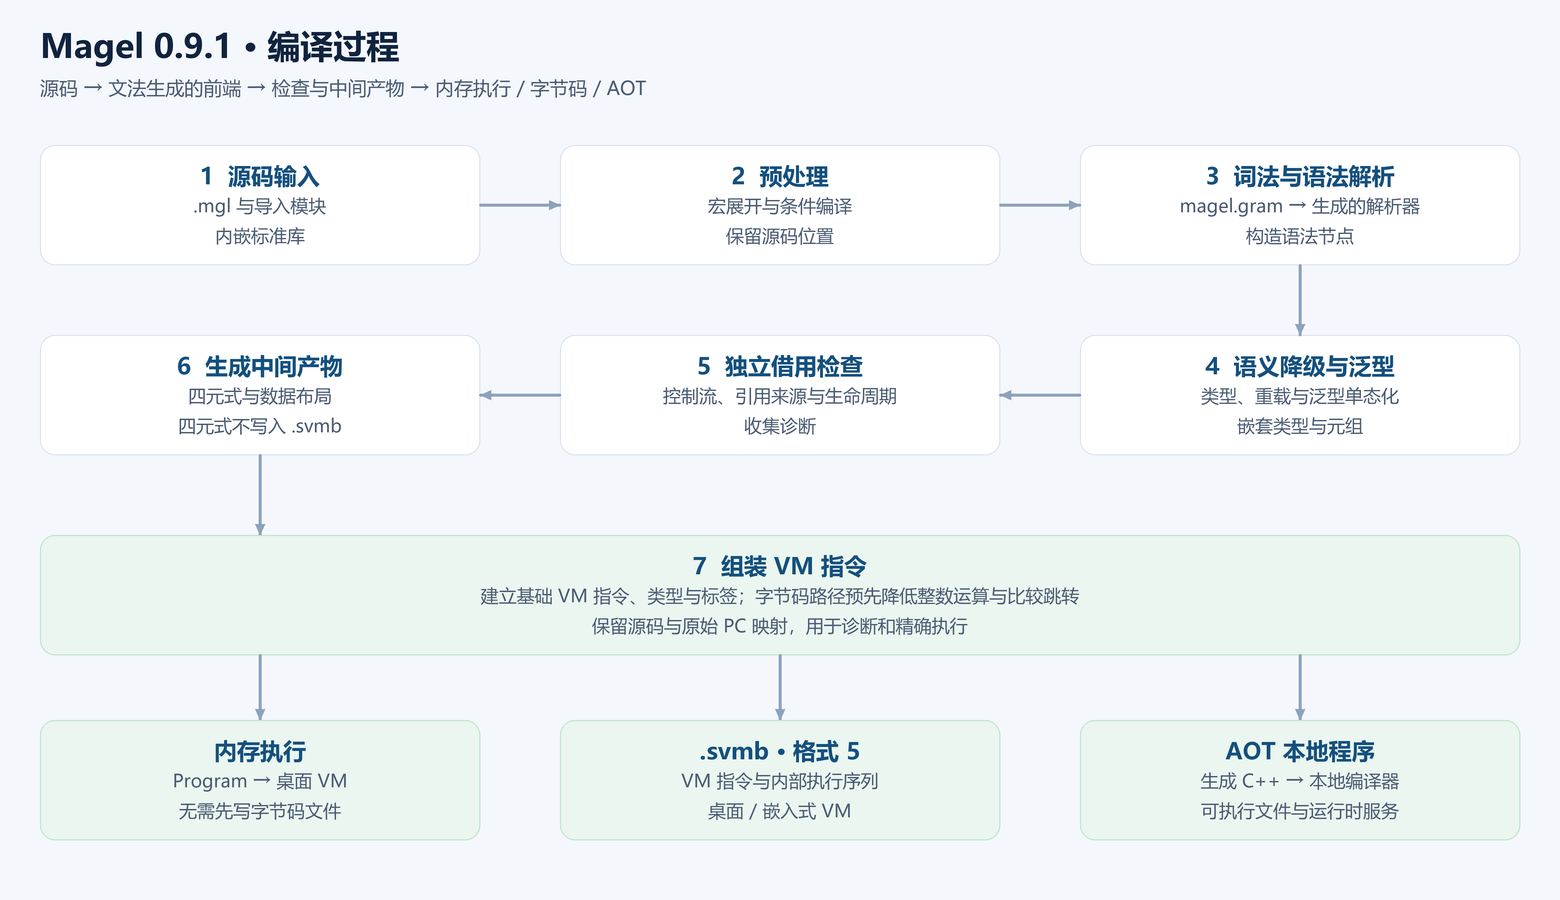
\includegraphics[width=\linewidth]{../images/magel-compilation.png}\par
Magel 编译流程：预处理、解析、语义期宏展开、借用检查、四元式及 VM 装配
\end{center}

四元式是本书所说的 IR。编译器先生成四元式、数据区和布局，供检查或后续装配；执行路径对四元式进行完整优化，再组装 VM 指令。图中的四元式产物出口位于生成阶段，优化结果可通过调试输出检查，二者不要混淆。

再看运行流程。源码运行和字节码运行最终都进入同一套共享 VM。执行准备绑定入口和宿主服务，运行时按指令操作数据、调用原生服务，并处理预算、错误与资源清理。

\begin{center}
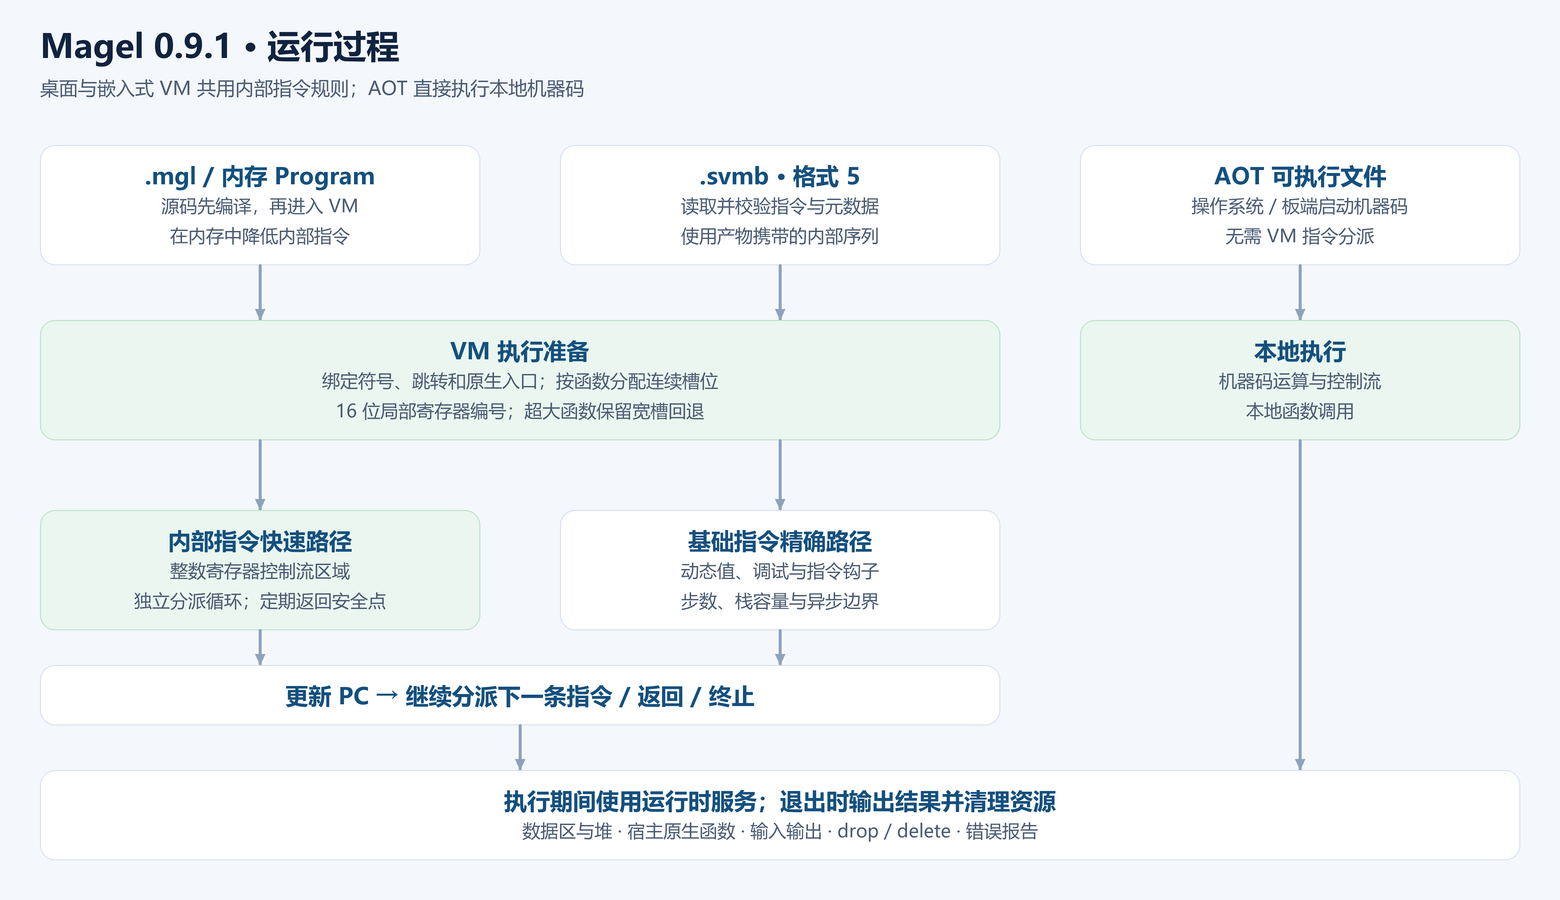
\includegraphics[width=\linewidth]{../images/magel-execution.png}\par
Magel 虚拟机流程：程序加载、执行准备、寄存器快速路径、精确路径与运行时服务
\end{center}

寄存器核心、融合与其他优化属于 VM 内部实现；调试和精确边界按需要使用相应路径。使用者先关注输入、输出和错误，不必在第一章记住所有实现名词。资源与作用域见第 8 章，实际交付边界见第 22 章。

两张图与仓库 README 使用相同绘图脚本生成。内嵌手册导出时携带图片，PDF 也直接收录图片，所以离线阅读不依赖网络。

\section{小结}

这一章你认识了：

\begin{itemize}

\item 入口函数固定叫 \texttt{main}，返回 \texttt{int64} 或 \texttt{void}；\texttt{void main} 正常完成时退出码为 0，panic 仍失败；

\item \texttt{println(\allowbreak{}.\allowbreak{}.\allowbreak{}.\allowbreak{})\allowbreak{}} 打印一行，来自核心库，不用 import；

\item 分号断句、花括号划范围，和 C 系语言一样；

\item \texttt{magel run} 跑，\texttt{magel check} 只查；

\item 报错会给出行列位置和画了波浪线的源码，而且大多在编译期就报出来了。

\end{itemize}

还有一件事本章没讲：\texttt{println} 为什么不用 \texttt{import}？因为它属于核心模块 \texttt{lang}，而 \texttt{lang} 是自动加载的。别的模块就没这个待遇了，第 18 章会讲清楚。

\section{下一步}

光看「Hello, Magel」是学不会编程的。下一章我们写一个真的有用的小程序：键盘猜数字。它会用到变量、输入、循环和分支——四个最基础的积木，而且你会看到它们是怎么串在一起的。

翻到\hyperref[ch:02]{第 2 章 猜数字}。

\section{边界与验证}

通过语法和类型检查，只能证明对应静态检查通过。程序是否产生预期输出、是否访问了外部资源，需要运行验证；外部输入变化也可能使后续运行失败。

\section{习题}

前两题用于理解和基本实现，第三题检查边界，最后一题为综合挑战。先独立完成，再核对参考解答。

\begin{enumerate}

\item 解释检查成功与运行结果正确之间的区别。

\item 把欢迎程序改为输出两行，分别为自己的名字和 Hello, Magel!。

\item 删掉语句末尾的分号，检查诊断位置，再修复。

\item 挑战：写出一个检查成功、运行时断言失败的完整程序。

\end{enumerate}

\subsection*{参考解答与验收要点}

\begin{enumerate}

\item 检查不执行全部业务路径；运行时还可能发生断言、输入或宿主错误。至少分别记录检查状态、退出状态和实际输出。

\item 使用两次 println，逐行对照输出；不要把编辑器显示的文字当成程序输出。

\item 这是语法错误练习，应在检查阶段失败。记录文件、行列和具体缺失内容，不把整条诊断文案写死。

\item 在 main 内调用 assert(false)，检查成功但执行失败；将它作为故意失败用例单独保存。

\end{enumerate}

\section{番外：皇帝的新程序}

改编自安徒生《皇帝的新装》，以下为编程主题的独立改写。

皇帝最爱新程序，早朝先问今日添了几个功能。两个裁缝进宫，说能编出天下最快的程序，只有不称职的大臣看不见运行结果。

老臣奉命验收，看见屏幕空空，心中一惊。他问裁缝为何没有输出。裁缝指着一页没有错误的检查记录：“只有懂编译的人才看得出。”老臣便在验收书上写了“运行极快”。

第二位大臣更谨慎，亲眼看见源码通过检查，才回去报告：“臣已确认，全无错误。”他没有按下运行键，怕显得自己不懂。

游行那天，皇帝抱着空屏幕走过大街。百姓都赞叹程序的速度；一个孩子问：“它究竟做了什么？”人群渐渐安静。皇帝叫人运行，屏幕这才显出第一行字。他想停下游行，可仪仗已经走到了街口，大臣们仍举着写有“验收通过”的牌子。

\subsection*{技术对照}

通过语法和类型检查，只能证明对应静态检查通过。程序是否产生预期输出、是否访问了外部资源，需要运行验证；外部输入变化也可能使后续运行失败。
   % 第一个程序
\chapter{猜数字}
\label{ch:02}

第 1 章的程序只会说一句话。这一章我们要写一个真的会跟你对话的东西：

\begin{tip}{提示}
程序想一个 1 到 100 之间的整数，你输入猜测，它告诉你「太大」还是「太小」，直到你猜中为止，然后告诉你一共猜了几次。
\end{tip}

这个程序只用四个最基础的积木：变量、输入、分支、循环。我们把它们一块一块拼起来——每一步都能单独跑，你随时可以停下来看。

\begin{tip}{提示}
本章的代码建议你真的敲一遍。后面所有章节都建立在这一章的四种积木上。
\end{tip}

\section{第一步：先让它说一句话}

先别管猜数字，先让程序开口：

\par
\medskip
\begin{lstlisting}[style=magel]
int64 main()
{
    println("我想好了一个 1 到 100 的数，你猜是多少？");
    return 0;
}
\end{lstlisting}
\par
\medskip

\par
\medskip
\begin{lstlisting}[style=out]
我想好了一个 1 到 100 的数，你猜是多少？
\end{lstlisting}
\par
\medskip

没有新东西。就一句 \texttt{println}。

\section{第二步：读一个数进来}

光说话不够，它得能听见你。改一下：

\par
\medskip
\begin{lstlisting}[style=magel]
int64 main()
{
    println("我想好了一个 1 到 100 的数，你猜是多少？");
    int64 guess = inputInt();
    println("你猜的是 {}。", guess);
    return 0;
}
\end{lstlisting}
\par
\medskip

运行（\texttt{--input} 后面的内容就是喂给程序的标准输入）：

\par
\medskip
\begin{lstlisting}[style=sh]
magel run guess.mgl --input "42"
\end{lstlisting}
\par
\medskip

\par
\medskip
\begin{lstlisting}[style=out]
我想好了一个 1 到 100 的数，你猜是多少？
你猜的是 42。
\end{lstlisting}
\par
\medskip

三件新东西，一个一个说。

\texttt{int64 guess =\allowbreak{} input\allowbreak{}Int(\allowbreak{})\allowbreak{};} —— 读一个整数。

\texttt{input\allowbreak{}Int} 会去读用户输入的一项（用空白分隔），按 \texttt{int64} 解析，然后把值交出来。如果输入的不是合法整数，程序会在那里停下来报错，不会给你一个莫名其妙的 0。这一点和第 3 章要讲的「不隐式转换」是同一种性格：宁可当场停下，不猜你的意思。

核心模块 \texttt{lang} 会自动加载，\texttt{input\allowbreak{}Int} 和 \texttt{println} 都可以直接使用。示例优先写简短名称；只有同名符号发生冲突，或需要说明名称来源时，才使用 \texttt{std:\allowbreak{}:\allowbreak{}lang:\allowbreak{}:\allowbreak{}input\allowbreak{}Int}、\texttt{std:\allowbreak{}:\allowbreak{}lang:\allowbreak{}:\allowbreak{}println} 这样的完整名称。

\texttt{"你猜的是 \{\}。"} —— \texttt{\{\}} 是位置占位符。

\texttt{\{\}} 会按实参类型填入值，不需要额外写数值类型标记。占位符的格式与实参类型由编译器检查；本章示例统一使用 \texttt{\{\}}。

\section{第三步：比一比，给个提示}

现在让它知道答案是 42，并且判断你的猜测：

\par
\medskip
\begin{lstlisting}[style=magel]
int64 main()
{
    int64 secret = 42;
    println("我想好了一个 1 到 100 的数，你猜是多少？");
    int64 guess = inputInt();
    if (guess < secret)
    {
        println("太小了。");
    }
    elif (guess > secret)
    {
        println("太大了。");
    }
    else
    {
        println("猜对了！");
    }
    return 0;
}
\end{lstlisting}
\par
\medskip

输入 \texttt{50}：

\par
\medskip
\begin{lstlisting}[style=out]
我想好了一个 1 到 100 的数，你猜是多少？
太大了。
\end{lstlisting}
\par
\medskip

\texttt{int64 secret =\allowbreak{} 42;} 定义了一个变量：类型 \texttt{int64}、名字 \texttt{secret}、初始值 \texttt{42}。这里的 \texttt{=\allowbreak{}} 是赋值，不是数学上的「相等」。第 6 章你会知道它到底做了什么。

\texttt{if /\allowbreak{} elif /\allowbreak{} else} 就是分支。注意两点：

\begin{itemize}

\item 条件是写在括号里的，和 C 一样：\texttt{if (\allowbreak{}guess <\allowbreak{} secret)\allowbreak{}}；

\item 「否则如果」在 Magel 里拼作 \texttt{elif}，不是 \texttt{else if}，也不是 \texttt{elsif}。

\end{itemize}

每个分支的主体都要用 \texttt{\{ \}} 包起来。哪怕只有一句，也要包——Magel 没有「不写花括号只作用一行」那套规矩，省下的这点字换来的是不会看错的结构。

\section{第四步：让它一直问下去}

一次猜不中就要再来一次。把「读 + 判断」塞进一个循环：

\par
\medskip
\begin{lstlisting}[style=magel]
int64 main()
{
    int64 secret = 42;
    println("我想好了一个 1 到 100 的数，你猜是多少？");
    while (true)
    {
        int64 guess = inputInt();
        if (guess < secret)
        {
            println("太小了。");
        }
        elif (guess > secret)
        {
            println("太大了。");
        }
        else
        {
            println("猜对了！");
            break;
        }
    }
    return 0;
}
\end{lstlisting}
\par
\medskip

输入 \texttt{50 30 42}：

\par
\medskip
\begin{lstlisting}[style=out]
我想好了一个 1 到 100 的数，你猜是多少？
太大了。
太小了。
猜对了！
\end{lstlisting}
\par
\medskip

\texttt{while (\allowbreak{}true)\allowbreak{} \{ .\allowbreak{}.\allowbreak{}.\allowbreak{} \}} 是「只要条件成立就一直做」。条件是 \texttt{true}，字面意思就是永远成立——所以这个循环本身不会自己停。

\texttt{break;} 就是那个出口：猜对时跳出去。

\begin{tip}{提示}
有没有更贴切的写法？有。当循环的唯一出路是 \texttt{break} 时，Magel 允许你写\texttt{loop \{ .\allowbreak{}.\allowbreak{}.\allowbreak{} \}}，意思和 \texttt{while (\allowbreak{}true)\allowbreak{}} 一样，但一眼就能看出「这是个靠 \texttt{break} 结束的循环」。第 5 章会讲 \texttt{loop} 的另一个用法：带着值跳出来。
\end{tip}

顺便说明一个容易踩的点：变量 \texttt{guess} 在每次循环里都是新的。写在 \texttt{while} 里面的声明，每转一圈都会重新做一次。所以它不是「上一轮的 \texttt{guess} 被改掉」，而是「新一轮又创了一个 \texttt{guess}」。第 8 章会讲清这种「出作用域就消失」的规则。

\section{第五步：让答案真的随机}

固定答案 42 只能骗自己。要随机数，得请标准库帮忙：

\par
\medskip
\begin{lstlisting}[style=magel]
import std::random;

int64 main()
{
    Random gen = Random::withSeed((uint64)2026);
    int64 secret = gen.nextInt(1, 100);
    println("答案是 {}。", secret);
    return 0;
}
\end{lstlisting}
\par
\medskip

\par
\medskip
\begin{lstlisting}[style=out]
答案是 62。
\end{lstlisting}
\par
\medskip

四件事：

\texttt{import std:\allowbreak{}:\allowbreak{}random;} —— 把标准库的 \texttt{random} 模块引进来。除了核心模块 \texttt{lang} 之外的模块，都要显式 \texttt{import}（第 18 章）。

\texttt{Random gen =\allowbreak{} .\allowbreak{}.\allowbreak{}.\allowbreak{}} —— \texttt{Random} 是一个结构体（struct），你可以先把它当成「一个装着随机数发生器的小盒子」。结构体在第 9 章细讲。

\texttt{Random:\allowbreak{}:\allowbreak{}with\allowbreak{}Seed(\allowbreak{}(\allowbreak{}uint64)\allowbreak{}2026)\allowbreak{}} —— \texttt{:\allowbreak{}:\allowbreak{}} 表示调这个类型上的静态方法。\texttt{with\allowbreak{}Seed} 是「用指定种子造一个发生器」。

那个 \texttt{(\allowbreak{}uint64)\allowbreak{}} 强转是必需的，不是装饰。 \texttt{2026} 这个字面量默认是 \texttt{int64}，而 \texttt{with\allowbreak{}Seed} 要的是 \texttt{uint64}；Magel 不做隐式转换，你不写它就编译不过：

\par
\medskip
\begin{lstlisting}[style=out]
magel：调用 static 函数 Random::withSeed 找不到匹配的重载：(int64)；没有参数类型能对上的重载（候选：Random.withSeed）
\end{lstlisting}
\par
\medskip

第一次遇到会觉得它死板。但换个角度：报错说「我找不到 \texttt{(\allowbreak{}int64)\allowbreak{}} 的重载」，它把它拿到了什么告诉你了。第 3 章会专门讲这套转换规则。

为什么用种子，不用真随机？ 因为要能复现。

\texttt{with\allowbreak{}Seed(\allowbreak{}2026)\allowbreak{}} 每跑一次都给你同一串数，所以本书能写死「答案是 62」，你照着敲也能得到 62。真实程序里想要每次都不一样，就用：

\par
\medskip
\begin{lstlisting}[style=magel]
Random gen = Random::fromEntropy();
\end{lstlisting}
\par
\medskip

\section{完整程序}

把上面五步合起来：

\par
\medskip
\begin{lstlisting}[style=magel]
import std::random;

int64 main()
{
    Random gen = Random::withSeed((uint64)2026);
    int64 secret = gen.nextInt(1, 100);
    int64 tries = 0;

    println("我想好了一个 1 到 100 的数，你猜是多少？");
    while (true)
    {
        int64 guess = inputInt();
        tries = tries + 1;
        if (guess < secret)
        {
            println("太小了。");
        }
        elif (guess > secret)
        {
            println("太大了。");
        }
        else
        {
            println("猜对了！答案是 {}，你用了 {} 次。", secret, tries);
            break;
        }
    }
    return 0;
}
\end{lstlisting}
\par
\medskip

\par
\medskip
\begin{lstlisting}[style=sh]
magel run guess.mgl --input "50 75 62"
\end{lstlisting}
\par
\medskip

\par
\medskip
\begin{lstlisting}[style=out]
我想好了一个 1 到 100 的数，你猜是多少？
太小了。
太大了。
猜对了！答案是 62，你用了 3 次。
\end{lstlisting}
\par
\medskip

新东西只有一处：\texttt{tries =\allowbreak{} tries + 1;}

这行读作「\texttt{tries} 变成它原来的值加一」。\texttt{=\allowbreak{}} 依然是赋值。Magel 也支持写成 \texttt{tries +=\allowbreak{} 1;}（第 5 章会讲这一串复合赋值），但本书前面会一直用 \texttt{tries =\allowbreak{} tries + 1} 这种最直白的写法——先写清楚，再写短。

顺带一提：\texttt{++tries} 那种自增写法 Magel 也有，但它对「同一个变量在一个表达式里被读写两次」管得很严，用不好会直接报错。第 5 章再说。

\section{出错的时候}

这个程序很容易出错，两种错法都很典型。

输入不够。 程序要两个数，你只给了一个：

\par
\medskip
\begin{lstlisting}[style=magel]
int64 main()
{
    int64 first = inputInt();
    int64 second = inputInt();
    println("{} {}", first, second);
    return 0;
}
\end{lstlisting}
\par
\medskip

\par
\medskip
\begin{lstlisting}[style=out]
magel：运行期错误：输入不够（第 2 项缺失）
出错位置：guess.mgl:3（main）
调用栈（外 → 内）：
  main  guess.mgl:3 [thread 0 coroutine 0 ip 3]
\end{lstlisting}
\par
\medskip

输入不是整数。

\par
\medskip
\begin{lstlisting}[style=magel]
int64 main()
{
    int64 value = inputInt();
    println("{}", value);
    return 0;
}
\end{lstlisting}
\par
\medskip

\par
\medskip
\begin{lstlisting}[style=out]
magel：运行期错误：std::lang::inputInt 读到的不是合法 int："abc"
出错位置：guess.mgl:2（main）
调用栈（外 → 内）：
  main  guess.mgl:2 [thread 0 coroutine 0 ip 3]
\end{lstlisting}
\par
\medskip

注意这两条报错和上一章那条语法错误的区别：

\begin{center}
\begin{tabular}{lll}
\toprule
 & 什么时候报 & 谁的问题 \\
\midrule
\texttt{语法错误：…} & 编译期，程序一个字符都没跑 & 代码写错了 \\
\texttt{magel：运行期错误：…} & 运行期，跑到那一句才炸 & 数据不合法 \\
\bottomrule
\end{tabular}
\end{center}

Magel 的立场是：代码的错误要尽量在编译期抓干净。所以「类型对不上」是编译期的事，而「用户输入了个 \texttt{abc}」只能运行期知道——这种事它只能诚实地停下来，并告诉你停在哪一行。

程序停下来的位置写成了 \texttt{guess.\allowbreak{}mgl:\allowbreak{}9}，连调用栈都给了；写大程序时这东西能救你。

\section{小结}

这一章你认识了四种积木，还有几个语法细节：

\begin{center}
\begin{tabular}{ll}
\toprule
你会了 & 关键点 \\
\midrule
变量 & \texttt{int64 secret =\allowbreak{} 42;} —— 类型写在名字前面 \\
输入 & \texttt{input\allowbreak{}Int(\allowbreak{})\allowbreak{}} 读一个整数，读不合法就报错 \\
分支 & \texttt{if (\allowbreak{}…)\allowbreak{} \{ \} elif (\allowbreak{}…)\allowbreak{} \{ \} else \{ \}}，主体必须带花括号 \\
循环 & \texttt{while (\allowbreak{}true)\allowbreak{} \{ … break; \}} \\
格式化 & \texttt{\{\}} 是位置占位符，类型由实参推导 \\
模块 & \texttt{import std:\allowbreak{}:\allowbreak{}random;}；只有 \texttt{lang} 是自动加载的 \\
静态方法 & \texttt{Random:\allowbreak{}:\allowbreak{}with\allowbreak{}Seed(\allowbreak{}.\allowbreak{}.\allowbreak{}.\allowbreak{})\allowbreak{}}，\texttt{:\allowbreak{}:\allowbreak{}} 后面是类型级的东西 \\
强转 & \texttt{(\allowbreak{}uint64)\allowbreak{}2026} —— Magel 不做隐式转换 \\
\bottomrule
\end{tabular}
\end{center}

还有一个习惯要开始养成：先 \texttt{check} 再 \texttt{run}。

\par
\medskip
\begin{lstlisting}[style=sh]
magel check guess.mgl    # 只查语法和类型，不执行
\end{lstlisting}
\par
\medskip

\section{下一步}

第 2 章里我们「先用后解释」了不少东西——变量到底是什么、为什么 \texttt{2026} 不能直接交给 \texttt{with\allowbreak{}Seed}、\texttt{\{\}} 是怎么知道该打印成整数的。

下一章就来补上最基础的一块：变量与类型。

翻到\hyperref[ch:03]{第 3 章 变量与类型}。
   % 猜数字

\chapter{变量与类型}
\label{ch:03}

第 1、2 章你已经写过不少变量了，但都是「照抄」。这一章把它讲清楚：

\begin{itemize}

\item 变量是什么、为什么每个变量都要写类型；

\item Magel 有哪些基础类型；

\item 数字、字符、字符串分别怎么写；

\item 以及本章的重头戏：Magel 什么时候替你转类型、什么时候非要你签字。

\end{itemize}

这一章会让你第一次觉得 Magel「有点死板」。请忍着别关页面——第 3.8 节会把这份死板值不值讲清楚。

\section{变量：给值起个名字}

\par
\medskip
\begin{lstlisting}[style=magel]
int64 score = 30;
\end{lstlisting}
\par
\medskip

这一行的读法从左到右：

\begin{center}
\begin{tabular}{ll}
\toprule
部分 & 含义 \\
\midrule
\texttt{int64} & 类型：这个变量装 64 位有符号整数 \\
\texttt{score} & 名字：你自己起的，区分大小写 \\
\texttt{=\allowbreak{}} & 赋值：把右边算出来的值放进这个变量 \\
\texttt{30} & 初始值 \\
\bottomrule
\end{tabular}
\end{center}

类型写在名字前面，这是 C / Java / C++ 的习惯，不是 Rust / TypeScript 那种\texttt{score:\allowbreak{} int64} 或者 \texttt{let score}。和 C 系一样的写法是故意的：Magel 不打算让你重新学一遍已经会的东西。

三个必须记住的细节：

\begin{enumerate}

\item 分号结尾。Magel 不用换行来表示语句结束，写成一整行也行。

\item 区分大小写。\texttt{score} 和 \texttt{Score} 是两个不同的名字。

\item 变量必须先声明再用。写到没声明过的名字是编译错误，不是「默认 0」。

\end{enumerate}

\section{为什么非要写类型}

很多现代语言会帮你推：\texttt{let score =\allowbreak{} 30} 就够了。Magel 能推（下一节就讲 \texttt{auto}），但声明时默认要求你写出来。理由和它的整体性格一致：

\begin{itemize}

\item 读代码的人不用猜。 \texttt{int64 score =\allowbreak{} get\allowbreak{}Score(\allowbreak{})\allowbreak{};} 一眼就知道这里是整数；\texttt{let score =\allowbreak{} get\allowbreak{}Score(\allowbreak{})\allowbreak{}} 得跳去看 \texttt{get\allowbreak{}Score} 的签名。

\item 它不猜你的意思。 记住第 2 章那条报错——\texttt{2026} 不能直接交给要 \texttt{uint64} 的函数。Magel 宁可让你写一个 \texttt{(\allowbreak{}uint64)\allowbreak{}}，也不愿意在某处悄悄换一下。

\item 出错点离原因近。 类型写错，报错就在那一行；不写类型，错可能传到十层外面才炸。

\end{itemize}

\section{整型家族}

\par
\medskip
\begin{lstlisting}[style=magel]
int64 main()
{
    int8 tiny = 127;
    int32 normal = 70000;
    int64 huge = 9000000000;
    uint8 byte = 255;
    println("{} {} {} {}", tiny, normal, huge, byte);
    return 0;
}
\end{lstlisting}
\par
\medskip

\par
\medskip
\begin{lstlisting}[style=out]
127 70000 9000000000 255
\end{lstlisting}
\par
\medskip

\begin{center}
\begin{tabular}{llll}
\toprule
有符号 & 无符号 & 位数 & 大概装得下 \\
\midrule
\texttt{int8} & \texttt{uint8} & 8 & ±127 / 0 到 255 \\
\texttt{int16} & \texttt{uint16} & 16 & ±32767 / 0 到 65535 \\
\texttt{int32} & \texttt{uint32} & 32 & ±21 亿 / 0 到 42 亿 \\
\texttt{int64} & \texttt{uint64} & 64 & ±9.2\ensuremath{\times}10¹⁸ —— 默认选手 \\
\bottomrule
\end{tabular}
\end{center}

日常直接用 \texttt{int64}。 只有两种情况才去挑更窄的：

\begin{itemize}

\item 要跟硬件、文件格式、二进制协议对齐（这时你知道必须是 8 位还是 16 位）；

\item 要省内存（嵌入式板子上，一个 8 位字段和 64 位字段差 8 倍）。

\end{itemize}

为什么没有 \texttt{int}、\texttt{long} 这种名字？ 因为那些名字的含义会随平台变，而这门语言要「一份逻辑从 MCU 跑到云端」——平台上不确定的东西，类型里不能含糊。

\section{浮点}

\par
\medskip
\begin{lstlisting}[style=magel]
int64 main()
{
    float64 ratio = 3.25;
    float32 single =(float32)1.5;
    println("{} {}", ratio, single);
    return 0;
}
\end{lstlisting}
\par
\medskip

\par
\medskip
\begin{lstlisting}[style=out]
3.25 1.5
\end{lstlisting}
\par
\medskip

\texttt{float64}（双精度）是默认选手，\texttt{float32}（单精度）在数值算法、图形、嵌入式里省内存时用。

\texttt{float64} 一栏里那个 \texttt{(\allowbreak{}float32)\allowbreak{}} 是必需的——直接写 \texttt{float32 single =\allowbreak{} 1.\allowbreak{}5;} 会报「不能隐式转换：float64 -> float32」。原因见第 3.8 节：字面量 \texttt{1.\allowbreak{}5} 的类型是\texttt{float64}，往更窄的类型里放就得自己签字。

\begin{tip}{一个容易上当的地方}
\texttt{123456789.\allowbreak{}0} 打印出来是 \texttt{1.\allowbreak{}23e+08}，\texttt{1000000000.\allowbreak{}0} 打印出来是 \texttt{1e+09}。浮点打印会走「短」的那条路，别拿它当精确输出用。要定格式，用 \texttt{format} 的样式参数（第 12 章）。
\end{tip}

\section{\texttt{bool}、\texttt{char}、\texttt{String}}

\par
\medskip
\begin{lstlisting}[style=magel]
int64 main()
{
    bool ready = true;
    bool done = false;
    char initial = 'M';
    String word = "Magel";
    println("{} {} {} {}", ready, done, initial, word);
    return 0;
}
\end{lstlisting}
\par
\medskip

\par
\medskip
\begin{lstlisting}[style=out]
1 0 M Magel
\end{lstlisting}
\par
\medskip

注意第一眼就有点怪的地方：\texttt{bool} 打印出来是 \texttt{1} 和 \texttt{0}，不是 \texttt{true} / \texttt{false}。它不是「字符串化的布尔」，打印时当整数处理了。要比对文本，得自己拼：

\par
\medskip
\begin{lstlisting}[style=magel]
int64 main()
{
    bool ready = true;
    String label;
    if (ready)
    {
        label = "yes";
    }
    else
    {
        label = "no";
    }
    println("{}", label);
    return 0;
}
\end{lstlisting}
\par
\medskip

\par
\medskip
\begin{lstlisting}[style=out]
yes
\end{lstlisting}
\par
\medskip

\begin{tip}{C 程序员注意}
Magel 没有三目运算符。写 \texttt{ready ? "yes" :\allowbreak{} "no"} 是语法错误，老老实实用 \texttt{if /\allowbreak{} else}。可以使用 \texttt{if (\allowbreak{}条件)\allowbreak{} \{ 值一 \} else \{ 值二 \}} 条件表达式；只求值命中的分支。
\end{tip}

\begin{itemize}

\item \texttt{bool} 只有 \texttt{true} 和 \texttt{false} 两个字面量，没有「非零即真」：

\end{itemize}

\par
\medskip
\begin{lstlisting}[style=out]
magel：if 条件必须是 bool，现在给的是 int64（数值条件请显式写成 `(bool)值` 或比较表达式）
\end{lstlisting}
\par
\medskip

硬要拿数字当布尔，得签字写成 \texttt{(\allowbreak{}bool)\allowbreak{}值}——但十有八九你真正想要的是一个比较表达式。

\begin{itemize}

\item \texttt{char} 是单个字符，用单引号：\texttt{'M'}。它和整数不是一回事，\texttt{char c =\allowbreak{} 65;} 会报错，得写 \texttt{(\allowbreak{}char)\allowbreak{}65}。

\item \texttt{String} 是字符串，用双引号，类型是 \texttt{std:\allowbreak{}:\allowbreak{}lang:\allowbreak{}:\allowbreak{}String} 的简写。它属于核心模块 \texttt{lang}，所以不用 import。字符串的内容是第 12 章的主题。

\end{itemize}

\section{常量 \texttt{const} 与推导 \texttt{auto}}

\par
\medskip
\begin{lstlisting}[style=magel]
int64 main()
{
    const int64 LIMIT = 100;
    auto inferred = LIMIT;
    println("{} {}", LIMIT, inferred);
    return 0;
}
\end{lstlisting}
\par
\medskip

\par
\medskip
\begin{lstlisting}[style=out]
100 100
\end{lstlisting}
\par
\medskip

\texttt{const} 表示「这个值定下来就不改了」。给 const 变量再赋值是编译错误。数组长度、缓冲区大小这类东西应该写成 const——不是为了让编译器放心，是为了让下一个读代码的人放心。

\texttt{auto} 表示「类型你替我推」。什么时候用？当右边已经写得很清楚的时候：

\par
\medskip
\begin{lstlisting}[style=magel]
auto info = describe(7);
// 想省一次手写类型
auto picked = range(1, 6).map(square).collect();
// 类型根本写不出来
\end{lstlisting}
\par
\medskip

第二种情况才是 \texttt{auto} 真正的用武之地——后面第 14、17 章会出现那种「类型长得没法看、写出来反而更难读」的场合。

但别滥用。函数内部的小变量用 \texttt{auto} 无所谓，函数签名、结构体字段、全局变量一律写全类型。一句话：类型是给别人看的，不是给编译器看的。

\section{字面量怎么写}

\par
\medskip
\begin{lstlisting}[style=magel]
int64 main()
{
    println("{} {} {}", 0xFF, b1010, 3.14);
    println("{} {}", 2.5e3, 2.5e - 3);
    println("{}", 1e9);
    return 0;
}
\end{lstlisting}
\par
\medskip

\par
\medskip
\begin{lstlisting}[style=out]
255 10 3.14
2.5e+03 0.0025
1e+09
\end{lstlisting}
\par
\medskip

\begin{center}
\begin{tabular}{ll}
\toprule
写法 & 含义 \\
\midrule
\texttt{42} & 十进制整数 \\
\texttt{0x\allowbreak{}FF} & 十六进制（前缀 \texttt{0x}） \\
\texttt{b1010} & 二进制（前缀 \texttt{b}，不是 \texttt{0b}） \\
\texttt{3.\allowbreak{}14} & 浮点，默认 \texttt{float64} \\
\texttt{2.\allowbreak{}5e3} & 科学计数法：2500.0 \\
\texttt{1e9} & 科学计数法：10⁹（没有小数点也算浮点，只要有指数） \\
\texttt{'M'} & 字符（单引号） \\
\texttt{"\textbackslash\{\}n"} & 字符串（双引号），里面有转义 \\
\bottomrule
\end{tabular}
\end{center}

\begin{tip}{提示}
二进制的前缀是 \texttt{b} 而不是 \texttt{0b}：\texttt{b1010} 是 10，写 \texttt{0b1010} 会报词法错误。这条容易记混，见本章最后的表。\par 带指数的就是浮点。 \texttt{1e9} 和 \texttt{2.\allowbreak{}5e3} 一样是 \texttt{float64}，所以 \texttt{int64 x =\allowbreak{} 1e9;} 会报「不能隐式转换：float64 -> int64」——浮点往整数里放要签字（见 3.9 节）。
\end{tip}

\subsection{数字后缀：\texttt{1u} 与 \texttt{1.\allowbreak{}0f}}

小写 \texttt{u} 表示无符号整数；没有类型上下文时默认是 \texttt{uint64}。无符号目标类型可以按自己的位宽接收这个字面量，并检查取值范围。它不会隐式变成有符号整数，也不能对无符号字面量直接写一元负号。

小写 \texttt{f} 把浮点字面量定为 \texttt{float32}。不带后缀的 \texttt{1.\allowbreak{}0} 是 \texttt{float64}；\texttt{1f}、\texttt{1.\allowbreak{}0f}、\texttt{1e2f} 都是 float32 写法。后缀必须小写。

\par
\medskip
\begin{lstlisting}[style=magel]
int64 floatingKind(float32 value)
{
    return 32;
}

int64 floatingKind(float64 value)
{
    return 64;
}

uint64 unsignedValue(uint64 value)
{
    return value;
}

int64 main()
{
    auto one = 1u;
    auto single = 1.0f;
    uint8 narrow = 255u;
    uint64 maximum = 18446744073709551615u;
    println("{} {} {} {}", unsignedValue(one), floatingKind(single),
            floatingKind(1.0), narrow);
    println("{}", maximum);
    return 0;
}
\end{lstlisting}
\par
\medskip

\par
\medskip
\begin{lstlisting}[style=out]
1 32 64 255
18446744073709551615
\end{lstlisting}
\par
\medskip

\texttt{uint8 narrow =\allowbreak{} 256u;} 会因为超范围报错。\texttt{int64 signed\allowbreak{}Value =\allowbreak{} 1u;} 不能隐式转换，\texttt{-1u} 也会被拒绝；需要有符号负数时直接写 \texttt{-1}。\texttt{0xffu}、\texttt{b\_101u} 同样支持无符号后缀。十六进制和现有二进制写法支持数字间的下划线分隔，但十进制 \texttt{1\_000} 和 \texttt{0b1010} 并不是当前文法支持的写法。

\section{隐式转换：只放行「变宽」}

这是本章最重要的一节。

先说结论，别被别的语言带偏：Magel 只放行一类转换——「变宽」，也就是「目标装得下源、不会悄悄丢东西」的方向。反过来（变窄、有符号放进无符号、浮点放进整数、\texttt{char}/\texttt{bool} 跟整数互放）一律要你签字。所以准确的说法不是「没有隐式转换」，而是只放行「装得下」的那半边。

\par
\medskip
\begin{lstlisting}[style=magel]
int64 main()
{
    int32 a = 100;
    int64 b = a;
    // 整型同符号变宽，放行
    uint8 u = 200;
    int32 m = u;
    // 无符号 -> 更宽的有符号，放行
    float64 c = b;
    // 整型 -> 浮点，放行
    println("{} {} {}", b, m, c);
    return 0;
}
\end{lstlisting}
\par
\medskip

\par
\medskip
\begin{lstlisting}[style=out]
100 200 100
\end{lstlisting}
\par
\medskip

放行清单（不用签字）：

{\small\setlength{\tabcolsep}{4pt}
\begin{longtable}{>{\raggedright\arraybackslash}p{\dimexpr 0.269\linewidth-2\tabcolsep\relax}>{\raggedright\arraybackslash}p{\dimexpr 0.711\linewidth-2\tabcolsep\relax}}
\toprule
方向 & 例子 \\
\midrule
\endhead
同符号整型变宽 & \texttt{int8 → int16/\allowbreak{}int32/\allowbreak{}int64}、\texttt{int32 → int64}、\texttt{uint8 → uint32} …… \\
无符号 \ensuremath{\rightarrow} 更宽的有符号 & \texttt{uint8 → int16/\allowbreak{}int32/\allowbreak{}int64}、\texttt{uint16 → int32}、\texttt{uint32 → int64} \\
整型 \ensuremath{\rightarrow} 浮点 & \texttt{int64 → float64}、\texttt{int32 → float32} \\
浮点变宽 & \texttt{float32 → float64} \\
\bottomrule
\end{longtable}
}

下面这三类，方向是反的，必须自己签字：

\par
\medskip
\begin{lstlisting}[style=magel]
int64 main()
{
    int64 big = 70000;
    int32 small = big;
    // 缩窄：位宽变小
    println("{}", small);
    return 0;
}
\end{lstlisting}
\par
\medskip

\par
\medskip
\begin{lstlisting}[style=out]
magel：不能隐式转换：int64 -> int32（请显式强转）
\end{lstlisting}
\par
\medskip

\begin{itemize}

\item 缩窄：位宽变小（\texttt{int64 → int32}、\texttt{float64 → float32}、\texttt{uint8 → int8}）——装不下，要签字；

\item 有符号 \ensuremath{\rightarrow} 无符号：哪怕目标更宽也不行（\texttt{int32 → uint32}、\texttt{int64 → uint64}）——负数塞不进无符号，要签字；

\item 跨大类：浮点 \ensuremath{\rightarrow} 整型、\texttt{char} / \texttt{bool} \ensuremath{\leftrightarrow} 整型——含义会变，要签字。

\end{itemize}

\begin{tip}{提示}
一句话记法：装得下的方向，Magel 自动帮你；装不下、或者换符号/大类，必须你亲自签字。
\end{tip}

这么一管，麻烦是麻烦了点，但它买到的是三件事：

\begin{enumerate}

\item 每一处精度损失都是有意的。 \texttt{int64} 里装着 90 亿，你要往 \texttt{int32} 里塞——这一下你必然写了 \texttt{(\allowbreak{}int32)\allowbreak{}}，将来出了问题，你能顺着这个强转找到是谁决定的。

\item 重载能被准确选中。 第 2 章那条「找不到匹配的重载 \texttt{(\allowbreak{}int64)\allowbreak{}}」就是这套规则的副产品：因为不替你「凑合着转」，编译器只能说「你要 \texttt{uint64}，给我的是 \texttt{int64}」——它把真相告诉你了，而不是塞进某个它认为差不多的重载。

\item 跨平台的结果是确定的。 在 32 位板子上 \texttt{long} 是 4 字节、PC 上是 8 字节，这种「同一个表达式换台机器结果不同」的坑，Magel 用「类型必须对上」堵掉了。

\end{enumerate}

什么时候你会想骂它？ 写累加、写混合计算的时候。这时候记住两句话：

\begin{itemize}

\item 拿不准就用 \texttt{int64} / \texttt{float64}，让变量类型统一，转换就少了；

\item 真要转，把它写在最显眼的地方（用括号包住，别藏在表达式中间）。

\end{itemize}

\section{显式强转：\texttt{(\allowbreak{}目标类型)\allowbreak{}值}}

\par
\medskip
\begin{lstlisting}[style=magel]
int64 main()
{
    int64 big = 70000;
    int32 normal =(int32)big;
    uint8 byte =(uint8)300;
    char letter =(char)65;
    println("{} {} {}", normal, byte, letter);
    return 0;
}
\end{lstlisting}
\par
\medskip

\par
\medskip
\begin{lstlisting}[style=out]
70000 44 A
\end{lstlisting}
\par
\medskip

写法就是 C 的老规矩：在值前面用括号写上目标类型。

三行分别演示了三件事：

\begin{itemize}

\item \texttt{(\allowbreak{}int32)\allowbreak{}big} —— 缩窄。70000 装得进 \texttt{int32}，值不变。

\item \texttt{(\allowbreak{}uint8)\allowbreak{}300} —— 截断。300 装不进 8 位，只留下低 8 位，得到 \texttt{44}。强转不会帮你检查装得下装不下——签了字就由你负责。

\item \texttt{(\allowbreak{}char)\allowbreak{}65} —— 数字变字符，65 就是 \texttt{'A'}。

\end{itemize}

\begin{tip}{提示}
强转是「你签字、编译器照做」，不做范围检查。 所以 \texttt{(\allowbreak{}int8)\allowbreak{}200} 得到 \texttt{-56}、\texttt{(\allowbreak{}uint8)\allowbreak{}300} 得到 \texttt{44}，都不报错。会做范围检查的是字面量直接落进槽位那条路（3.10 节）——两条路泾渭分明：没写强转，编译器替你把关；写了强转，责任在你。
\end{tip}

反过来 \texttt{(\allowbreak{}int64)\allowbreak{}3.\allowbreak{}9} 得到 \texttt{1}：浮点转整数是直接砍掉小数位，不是四舍五入。要四舍五入得自己想办法（\texttt{std:\allowbreak{}:\allowbreak{}math} 里有取整函数，第 12 章提）。

\subsection{\texttt{cast<\allowbreak{}T>\allowbreak{}(\allowbreak{}value)\allowbreak{}}：把目标类型写清楚}

除了前面的 C 风格强转，也可以写 \texttt{cast<\allowbreak{}目标类型>\allowbreak{}(\allowbreak{}值)\allowbreak{}}。这是显式转换，不是允许普通赋值偷偷缩窄。

\par
\medskip
\begin{lstlisting}[style=magel]
int64 main()
{
    int64 original = 42;
    int32 narrowed = cast<int32>(original);
    println("{}", narrowed);
    return 0;
}
\end{lstlisting}
\par
\medskip

\par
\medskip
\begin{lstlisting}[style=out]
42
\end{lstlisting}
\par
\medskip

尖括号中是目标类型，圆括号中是被转换的表达式。自定义类型的显式转换要提供对应协议；宿主类型的 \texttt{impl} 绑定见第 21 章。转换也不会让一个引用越过来源的生命周期。

\section{字面量的取值范围}

这一节两条规矩，都是本书撰写时实测确认过的：

规矩一：负数字面量可以直接写进窄类型。

\texttt{-300} 在语法上是「一元负号 + 正数字面量 \texttt{300}」，但编译器把它当常量看值——只要值落在目标类型的范围内，就直接放行：

\par
\medskip
\begin{lstlisting}[style=magel]
int64 main()
{
    int16 small = -300;
    // -300 落在 int16（-32768..32767）里
    int8 tiny = -100;
    println("{} {}", small, tiny);
    return 0;
}
\end{lstlisting}
\par
\medskip

\par
\medskip
\begin{lstlisting}[style=out]
-300 -100
\end{lstlisting}
\par
\medskip

规矩二：十进制字面量超出范围会报错，不静默回绕。

\par
\medskip
\begin{lstlisting}[style=magel]
int64 main()
{
    int8 overflow = 200;
    // int8 只到 127
    return 0;
}
\end{lstlisting}
\par
\medskip

\par
\medskip
\begin{lstlisting}[style=out]
magel：整数字面量 200 超出 int8 的取值范围（-128..127）
\end{lstlisting}
\par
\medskip

\texttt{uint8 b =\allowbreak{} 255;} 没问题（255 在 \texttt{0.\allowbreak{}.\allowbreak{}255} 里），\texttt{uint8 b =\allowbreak{} 256;} 报同样的错。这条只管「字面量落进槽位」（初始化 / 赋值）；显式强转是另一回事——\texttt{(\allowbreak{}int8)\allowbreak{}200} 是你亲口签字，编译器只管按位截断（见 3.9 节）。

\begin{tip}{提示}
十六进制 / 二进制字面量按「位模式」处理，不做范围检查。 \texttt{int8 x =\allowbreak{} 0x\allowbreak{}FF;} 得到 \texttt{-1}（低 8 位全 1，按有符号读就是 -1），和 C 一样。要写明确的位模式，就用 \texttt{0x} / \texttt{b} 前缀。
\end{tip}

还有几个词法上的「不认」，撞上了照右列改：

\begin{center}
\begin{tabular}{lll}
\toprule
你可能想写 & 实际会怎样 & 改成 \\
\midrule
\texttt{0b1010} & 词法错误（前缀是 \texttt{b}，不是 \texttt{0b}） & \texttt{b1010} \\
\texttt{1\_000} & 语法错误（下划线分隔不认） & \texttt{1000} \\
\texttt{1.\allowbreak{}0F} / \texttt{1U} & 后缀必须小写 & \texttt{1.\allowbreak{}0f} / \texttt{1u} \\
\bottomrule
\end{tabular}
\end{center}

\section{小结}

{\small\setlength{\tabcolsep}{4pt}
\begin{longtable}{>{\raggedright\arraybackslash}p{\dimexpr 0.078\linewidth-2\tabcolsep\relax}>{\raggedright\arraybackslash}p{\dimexpr 0.902\linewidth-2\tabcolsep\relax}}
\toprule
你会了 & 关键点 \\
\midrule
\endhead
声明 & \texttt{int64 score =\allowbreak{} 30;}，类型在前、名字在后、分号结尾 \\
整型 & \texttt{int8/\allowbreak{}16/\allowbreak{}32/\allowbreak{}64} + \texttt{uint8/\allowbreak{}16/\allowbreak{}32/\allowbreak{}64}，日常用 \texttt{int64} \\
浮点 & 无后缀为 \texttt{float64}，\texttt{1.\allowbreak{}0f} 为 \texttt{float32}，也可显式转换 \\
其它标量 & \texttt{bool} 只有 \texttt{true/\allowbreak{}false}（打印成 1/0）、\texttt{char} 用单引号 \\
字符串 & \texttt{String} 用双引号，属核心模块 \texttt{lang}，不用 import \\
常量 & \texttt{const int64 LIMIT =\allowbreak{} 100;} \\
推导 & \texttt{auto}，适合右边已经把类型写清楚的场合 \\
字面量 & \texttt{0x\allowbreak{}FF}、\texttt{b1010}、\texttt{3.\allowbreak{}14}、\texttt{2.\allowbreak{}5e3}、\texttt{1e9}、\texttt{'M'}、\texttt{"\textbackslash\{\}n"} \\
转换 & 只放行装得下的方向（同符号整型变宽、无符号\ensuremath{\rightarrow}更宽的有符号、整\ensuremath{\rightarrow}浮、\texttt{float32}\ensuremath{\rightarrow}\texttt{float64}）；其余要显式强转 \texttt{(\allowbreak{}int64)\allowbreak{}x} \\
字面量范围 & 十进制字面量超范围直接报错（\texttt{int8 x =\allowbreak{} 200;} 不合法）；\texttt{0x}/\texttt{b} 字面量按位模式放行 \\
\bottomrule
\end{longtable}
}

一句话总结这一章：Magel 要把「类型在哪里变了」留成一件看得见的事。

\section{下一步}

现在你会声明变量、会算数，但所有代码都堆在 \texttt{main} 里。第 2 章那个猜数字程序要是再长一点，\texttt{main} 就没法看了。

下一章解决这个问题：把代码切成函数。

翻到\hyperref[ch:04]{第 4 章 函数}。
   % 变量与类型
\chapter{函数}
\label{ch:04}

第 2 章的猜数字程序全塞在 \texttt{main} 里。如果它再长三倍——比如加上「记录每次猜测」、「算平均猜几次」——\texttt{main} 就再也读不动了。

函数就是解决这个的：给一段代码起个名字，需要的时候叫它。

这一章讲清楚五件事：怎么定义、怎么传参、怎么返回、怎么重载、以及怎么一次返回好几个值。

\section{定义与调用}

\par
\medskip
\begin{lstlisting}[style=magel]
int64 add(int64 a, int64 b)
{
    return a + b;
}

void log(String message)
{
    println("[log] {}", message);
}

int64 main()
{
    log("start");
    println("{}", add(1, 2));
    return 0;
}
\end{lstlisting}
\par
\medskip

\par
\medskip
\begin{lstlisting}[style=out]
[log] start
3
\end{lstlisting}
\par
\medskip

拆开看一个函数的脑袋：

\par
\medskip
\begin{lstlisting}[style=out]
int64        add      ( int64 a , int64 b )   { ... }
 ↑            ↑         ↑
 返回类型     名字      参数表：每个参数都要写类型
\end{lstlisting}
\par
\medskip

\texttt{void} 表示「不返回东西」。 \texttt{log} 只做事、不交值，所以返回类型是 \texttt{void}。\texttt{void} 函数里不用写 \texttt{return}；想中途退出，写一个光秃秃的 \texttt{return;} 就行：

\par
\medskip
\begin{lstlisting}[style=magel]
void trace(int64 number)
{
    if (number < 0)
    {
        return;
        // 负数不看，直接走
    }
    println("n={}", number);
}
\end{lstlisting}
\par
\medskip

函数可以写在 \texttt{main} 前面或后面，Magel 不要求「先声明后使用」。这一点比 C 舒服——不用再维护一份头文件里的原型。

函数的顺序也有讲究，但不是给编译器的，是给读代码的人的：把「先读的放前面」。一般先放小工具，再放用它的人，最后才是 \texttt{main}。

\section{参数是副本}

这是本章最重要的一条规则，也是第 6 章那条大规则的小预告：

\par
\medskip
\begin{lstlisting}[style=magel]
void shout(String text)
{
    text = text + "!";
}

int64 main()
{
    String word = "hi";
    shout(word);
    println("{}", word);
    return 0;
}
\end{lstlisting}
\par
\medskip

\par
\medskip
\begin{lstlisting}[style=out]
hi
\end{lstlisting}
\par
\medskip

\texttt{shout} 里改了 \texttt{text}，\texttt{main} 里的 \texttt{word} 一点没变。

从 C++ / Java / Python 过来的人最容易在这里栽跟头：那些语言里字符串、对象传进去往往是「共享的引用」，函数里一改外面就变了。Magel 不是——传进去的是一份完整的副本。

想真的改到外面那个，得显式要求传引用（\texttt{T mut\&}），这是第 7 章的内容。现在你只要记住：函数的参数表就是「我复制这些值过来用」。

\begin{tip}{提示}
那大对象传进去岂不是很贵？是的，会很贵。这正是 Magel 让你自己决定的地方：不想复制就写 \texttt{String const\&}——一次显式的选择，而不是编译器偷偷替你优化。第 7 章会给出这几条写法的完整对照。
\end{tip}

\section{返回值}

\par
\medskip
\begin{lstlisting}[style=magel]
int64 clamp(int64 value)
{
    if (value < 0)
    {
        return 0;
    }
    return value;
}
\end{lstlisting}
\par
\medskip

\texttt{return} 后面跟的值的类型，必须和函数声明的返回类型一致，不允许隐式转换（还记得第 3 章那条规矩吧）。返回 \texttt{int64} 的函数不能 \texttt{return 3.\allowbreak{}5;}。

一个函数可以有多个 \texttt{return}——只要每条路都返回了一样类型的值。上面那个 \texttt{clamp} 有两条出路，都返回 \texttt{int64}。

如果一条路忘了返回呢？ 编译期就会报错，不会让你跑到一半发现「这个函数返回了垃圾」。

\subsection{返回一个带值的控制表达式}

\texttt{return} 后面既可以写普通值，也可以写块、\texttt{if}、\texttt{match} 或 \texttt{loop}。它们先给出一个结果，函数再返回这个结果。

\par
\medskip
\begin{lstlisting}[style=magel]
int64 fromBlock()
{
    return
    {
        int64 local = 3;
        yield local;
    };
}

int64 choose(bool first)
{
    return if (first)
    {
        yield 5;
    }
    else
    {
        yield 6;
    };
}

int64 fromMatch(int64 item)
{
    return match (item)
    {
        0 => { yield 7; }
        _ => { yield 8; }
    };
}

int64 fromLoop()
{
    return loop
    {
        yield 9;
    };
}

int64 main()
{
    println("{} {} {} {}", fromBlock(), choose(false), fromMatch(0), fromLoop());
    return 0;
}
\end{lstlisting}
\par
\medskip

\par
\medskip
\begin{lstlisting}[style=out]
3 6 7 9
\end{lstlisting}
\par
\medskip

这里的 \texttt{yield value;} 给出当前值表达式的结果，不是返回函数。只有表达式完成后，外层 \texttt{return} 才返回函数。所有可能给出结果的分支必须具有完全相同的类型；不能让一支是 \texttt{int32}、另一支是 \texttt{int64}，再指望编译器自动凑成同一种类型。

在这个返回表达式内部，不能再嵌套当前函数的 \texttt{return}，也不能使用 \texttt{break level N} / \texttt{break all} 跨层跳转；会提前返回的 \texttt{?} 同样需要改成显式匹配。表达式里新定义的独立函数有自己的返回边界。只含一个结果的 \texttt{\{ value \}} 分支仍可沿用前面的简写。

内部拥有值变量通过 \texttt{break} 交出结果时会隐式移动，外部变量仍按值复制。移动先保存结果，再执行离开作用域的清理；不会把已经交出去的值再析构一次。引用不能因此逃出来源的生命周期。第 8 章的清理规则和第 14 章的泛型返回会继续解释这些边界。

\section{重载：同名不同参}

同一个名字，可以按实参类型挑不同的实现：

\par
\medskip
\begin{lstlisting}[style=magel]
int64 add(int64 a, int64 b)
{
    return a + b;
}

float64 add(float64 a, float64 b)
{
    return a + b;
}

int64 main()
{
    println("{} {}", add(1, 2), add(1.5, 2.5));
    return 0;
}
\end{lstlisting}
\par
\medskip

\par
\medskip
\begin{lstlisting}[style=out]
3 4
\end{lstlisting}
\par
\medskip

选哪个是编译期定下来的，看实参类型：\texttt{add(\allowbreak{}1,\allowbreak{} 2)\allowbreak{}} 两个都是 \texttt{int64}，走第一份；\texttt{add(\allowbreak{}1.\allowbreak{}5,\allowbreak{} 2.\allowbreak{}5)\allowbreak{}} 两个都是 \texttt{float64}，走第二份。

这和第 3 章那条「没有隐式转换」是配套的：因为不做隐式转换，重载的挑选才是准的。 如果 \texttt{int64} 能自动变 \texttt{float64}，\texttt{add(\allowbreak{}1,\allowbreak{} 2.\allowbreak{}5)\allowbreak{}} 到底该走哪一份就得靠一套复杂的「谁更优」规则去猜了。Magel 的选择是：不猜，让你把类型写对。

找不到匹配的重载时，报错会把它拿到了什么类型和有哪些候选都列出来。比如只定义了 \texttt{int64} 的 \texttt{add}，却拿一个 \texttt{int64} 加一个 \texttt{float64} 去调：

\par
\medskip
\begin{lstlisting}[style=magel]
int64 add(int64 a, int64 b)
{
    return a + b;
}

int64 main()
{
    println("{}", add(1, 2.5));
    return 0;
}
\end{lstlisting}
\par
\medskip

\par
\medskip
\begin{lstlisting}[style=out]
magel：调用 函数 add 找不到匹配的重载：(int64, float64)；没有参数类型能对上的重载（候选：add）
\end{lstlisting}
\par
\medskip

看到这种错，先看括号里它拿到了什么类型，再决定是改实参还是加一份重载。（顺便：\texttt{2.\allowbreak{}5} 是 \texttt{float64}，\texttt{add(\allowbreak{}1,\allowbreak{} 2.\allowbreak{}5)\allowbreak{}} 里的 \texttt{1} 也不会被「凑」成 \texttt{float64}——回想第 3 章：没有隐式转换。）

\section{默认参数}

参数可以带默认值，调用时从尾部省略：

\par
\medskip
\begin{lstlisting}[style=magel]
int64 add(int64 a, int64 b = 10)
{
    return a + b;
}

int64 main()
{
    println("{} {}", add(2), add(2, 3));
    return 0;
}
\end{lstlisting}
\par
\medskip

\par
\medskip
\begin{lstlisting}[style=out]
12 5
\end{lstlisting}
\par
\medskip

两条规矩：

\begin{itemize}

\item 带默认值的参数必须排在后面并且连续——不能「第 1 个有默认值、第 2 个没有」：

\end{itemize}

\par
\medskip
\begin{lstlisting}[style=out]
magel：函数 add 的默认参数后不能有必填参数
\end{lstlisting}
\par
\medskip

\begin{itemize}

\item 省略时只能从尾部往前省。\texttt{add(\allowbreak{}2)\allowbreak{}} 省掉了 \texttt{b}，没问题；\texttt{add(\allowbreak{})\allowbreak{}} 不行，因为 \texttt{a} 没有默认值：

\end{itemize}

\par
\medskip
\begin{lstlisting}[style=out]
magel：调用 函数 add 找不到匹配的重载：()；没有参数类型能对上的重载（候选：add）
\end{lstlisting}
\par
\medskip

默认值在每次省略该参数时重新求值。所以别在默认值里写「记录调用次数」这种带副作用的表达式——每次都会算一遍。

\begin{tip}{提示}
什么时候用默认值？当一个参数大多数调用都会传同一个值，且传别的值不影响语义。比如 \texttt{add(\allowbreak{}a,\allowbreak{} b =\allowbreak{} 10)\allowbreak{}} 里的 \texttt{b} —— 它是「可选的微调」。反过来，一个「猜数字最大值」这种参数就别给默认值，因为给了等于偷偷替调用方做了决定。
\end{tip}

\section{变长参数}

最后一项参数可以写成 \texttt{T.\allowbreak{}.\allowbreak{}.\allowbreak{}}，表示「这里可以给任意多个」：

\par
\medskip
\begin{lstlisting}[style=magel]
int64 total(int64... items)
{
    int64 sum = 0;
    for (int64 item in items)
    {
        sum = sum + item;
    }
    return sum;
}

int64 main()
{
    println("{} {}", total(1, 2, 3), total(5));
    return 0;
}
\end{lstlisting}
\par
\medskip

\par
\medskip
\begin{lstlisting}[style=out]
6 5
\end{lstlisting}
\par
\medskip

\texttt{items} 在函数体里就是一个能遍历的容器。\texttt{for (\allowbreak{}int64 item in items)\allowbreak{}} 是「把 \texttt{items} 里的东西一个个拿出来，每轮叫它 \texttt{item}」——第 5 章细讲 \texttt{for-in}。

变长参数只能放在最后一项，而且一个函数只能有一处。

\section{一次返回多个值}

Magel 的返回值可以是一个元组（tuple）——把几个值打包起来：

\par
\medskip
\begin{lstlisting}[style=magel]
(int64, String) describe(int64 id)
{
    return(id, "player");
}

int64 main()
{
    auto info = describe(7);
    println("{} {}", info.0, info.1);
    return 0;
}
\end{lstlisting}
\par
\medskip

\par
\medskip
\begin{lstlisting}[style=out]
7 player
\end{lstlisting}
\par
\medskip

\begin{itemize}

\item 返回类型写成 \texttt{(\allowbreak{}int64,\allowbreak{} String)\allowbreak{}}，就是「一个 \texttt{int64} 加一个 \texttt{String}」；

\item \texttt{return (\allowbreak{}id,\allowbreak{} "player")\allowbreak{};} 把两个值打包成元组；

\item 取的时候用 \texttt{.\allowbreak{}0} / \texttt{.\allowbreak{}1} —— 这是位置，不是名字，从 0 开始数。

\end{itemize}

\texttt{return} 后面的括号可以省，\texttt{return id,\allowbreak{} "player";} 和上一种写法等价。

如果你不想用 \texttt{.\allowbreak{}0} / \texttt{.\allowbreak{}1}，可以直接拆开接：

\par
\medskip
\begin{lstlisting}[style=magel]
(int32, String) pair(int32 key, String name)
{
    return key, name;
}

int64 main()
{
    int32 key;
    String name;
    key, name = pair((int32)7, "player");
    println("{} {}", key, name);
    return 0;
}
\end{lstlisting}
\par
\medskip

\par
\medskip
\begin{lstlisting}[style=out]
7 player
\end{lstlisting}
\par
\medskip

这行 \texttt{key,\allowbreak{} name =\allowbreak{} pair(\allowbreak{}.\allowbreak{}.\allowbreak{}.\allowbreak{})\allowbreak{}} 的意思是：把右边元组按位置拆给左边的每一个目标。左边必须是已经声明过的变量——声明新变量请写 \texttt{auto (\allowbreak{}key,\allowbreak{} name)\allowbreak{} =\allowbreak{} pair(\allowbreak{}.\allowbreak{}.\allowbreak{}.\allowbreak{})\allowbreak{};}。

\begin{tip}{提示}
元组还能用来交换两个变量，而且不用中间变量：\texttt{x,\allowbreak{} y =\allowbreak{} (\allowbreak{}y,\allowbreak{} x)\allowbreak{};} —— 右边先整个求值一次，再逐个写回去。注意右边那个括号不能省，\texttt{x,\allowbreak{} y =\allowbreak{} y,\allowbreak{} x;} 会报「多目标解构赋值必须使用 \texttt{=\allowbreak{}} 和一个元组来源」。
\end{tip}

\section{入口 \texttt{main} 的两种形态}

到现在为止你写的都是不带参数的版本：

\par
\medskip
\begin{lstlisting}[style=magel]
int64 main()
{
    ...
}
\end{lstlisting}
\par
\medskip

要读命令行参数，换成另一种：

\par
\medskip
\begin{lstlisting}[style=magel]
int64 main(List<String> arguments)
{
    println("收到 {} 个参数", arguments.len());
    for (String item in arguments)
    {
        println("  {}", item);
    }
    return 0;
}
\end{lstlisting}
\par
\medskip

\par
\medskip
\begin{lstlisting}[style=out]
收到 2 个参数
  Alice
  two words
\end{lstlisting}
\par
\medskip

只有这两种入口是合法的，别自己发明第三种。

传参的写法要注意：直接给文件时，文件后面的都算程序参数。

\par
\medskip
\begin{lstlisting}[style=sh]
magel app.mgl Alice "two words"
\end{lstlisting}
\par
\medskip

但如果你把场景词 \texttt{run} 显式写出来，就得多一个 \texttt{--} 把「配置词」和「程序参数」隔开：

\par
\medskip
\begin{lstlisting}[style=sh]
magel run app.mgl -- Alice "two words"
\end{lstlisting}
\par
\medskip

不写 \texttt{--} 的话，\texttt{Alice} 会被当成另一个源文件，报「一次只能编译一个源文件」。

\section{小结}

\begin{center}
\begin{tabular}{ll}
\toprule
你会了 & 关键点 \\
\midrule
定义 & \texttt{int64 add(\allowbreak{}int64 a,\allowbreak{} int64 b)\allowbreak{} \{ return a + b; \}} \\
不返回值 & 返回类型写 \texttt{void}，里面可以 \texttt{return;} 提前退出 \\
调用 & 位置实参，从左往右一一对应 \\
参数语义 & 按值传入，形参是副本，改形参不影响调用方 \\
重载 & 同名不同参，编译期按实参类型选，报错会列出候选 \\
默认参数 & \texttt{int64 b =\allowbreak{} 10}，只能从尾部连续省略 \\
变长参数 & \texttt{int64.\allowbreak{}.\allowbreak{}.\allowbreak{} items}，放最后一项，用 \texttt{for-in} 遍历 \\
多值返回 & 返回类型写元组 \texttt{(\allowbreak{}A,\allowbreak{} B)\allowbreak{}}，用 \texttt{.\allowbreak{}0} / \texttt{.\allowbreak{}1} 取或拆开接 \\
入口 & \texttt{int64 main(\allowbreak{})\allowbreak{}} 或 \texttt{int64 main(\allowbreak{}std:\allowbreak{}:\allowbreak{}lang:\allowbreak{}:\allowbreak{}List<\allowbreak{}std:\allowbreak{}:\allowbreak{}lang:\allowbreak{}:\allowbreak{}String>\allowbreak{} arguments)\allowbreak{}} \\
\bottomrule
\end{tabular}
\end{center}

还有两处本章故意没讲透：

\begin{itemize}

\item \texttt{static} 方法（写在类型上、用 \texttt{Type:\allowbreak{}:\allowbreak{}method(\allowbreak{})\allowbreak{}} 调）和第 2 章那个\texttt{Random:\allowbreak{}:\allowbreak{}with\allowbreak{}Seed} —— 那是结构体的东西，第 9 章讲；

\item 把函数当值传递（\texttt{int64 fn(\allowbreak{}int64)\allowbreak{}} 类型、\texttt{fn}）—— 第 15 章讲。

\end{itemize}

\section{下一步}

现在你能把代码切成函数了，但函数里只能「从上往下一句句做」。真实程序还需要判断和重复——第 2 章你用过 \texttt{if} 和 \texttt{while}，但那是照着抄的。

下一章把控制流完整讲一遍，包括 \texttt{loop} 那个能「带值跳出来」的用法。

翻到\hyperref[ch:05]{第 5 章 控制流}。
   % 函数
\chapter{控制流}
\label{ch:05}

程序光会「从上往下做」是干不了活的。它得会拐弯（条件）和转圈（循环）。

第 2 章的猜数字已经把这两种都用上了，这一章把它们补全：ChaLi 一共有三种循环：\texttt{while}、\texttt{loop} 和 \texttt{for-in}，还有一套对「同一个变量在一个表达式里被读写两次」管得很严的规则。

\section{条件：\texttt{if} / \texttt{elif} / \texttt{else}}

\par
\medskip
\begin{lstlisting}[style=chali]
String classify(int64 value)
{
    if (value < 0)
    {
        return "负数";
    }
    elif (value == 0)
    {
        return "零";
    }
    else
    {
        return "正数";
    }
}

void main()
{
    println("{} {} {}", classify(-3), classify(0), classify(8));

}
\end{lstlisting}
\par
\medskip

\par
\medskip
\begin{lstlisting}[style=out]
负数 零 正数
\end{lstlisting}
\par
\medskip

形态就是这些：

\par
\medskip
\begin{lstlisting}[style=out]
if (条件) { ... }
elif (条件) { ... }
else { ... }
\end{lstlisting}
\par
\medskip

三条要注意的：

1. 条件必须真的能当条件。

\par
\medskip
\begin{lstlisting}[style=chali]
void main()
{
    if (1)
    {
        println("x");
    }

}
\end{lstlisting}
\par
\medskip

\par
\medskip
\begin{lstlisting}[style=out]
chali: if 条件必须是 bool，现在给的是 int64（数值条件请显式写成 `(bool)值` 或比较表达式）
\end{lstlisting}
\par
\medskip

没有「非零即真」。想判断「\texttt{count} 是不是 0」，写 \texttt{if (\allowbreak{}count !=\allowbreak{} 0)\allowbreak{}}——把你想说的说出来。

2. 拼写是 \texttt{elif}，不是 \texttt{else if}，也不是 \texttt{elsif}。少一个字母都编译不过。

3. 花括号不能省。 只写一句 \texttt{if (\allowbreak{}x)\allowbreak{} y =\allowbreak{} 1;} 是编译错误。这条和 C 不一样，但换来的是「这个 \texttt{y =\allowbreak{} 1} 到底属于哪个 if」永远不会有歧义。

\begin{tip}{提示}
ChaLi 没有三目运算符。 \texttt{cond ? a :\allowbreak{} b} 是语法错误（第 3 章提过）。简单替换就用 \texttt{if /\allowbreak{} else} 赋值；分支多了，第 10 章的 \texttt{match} 更好读。可以使用 \texttt{if (\allowbreak{}条件)\allowbreak{} \{ 值一 \} else \{ 值二 \}} 条件表达式；只求值命中的分支。
\end{tip}

\subsection*{条件也能产生值}

\texttt{if} 可以出现在变量定义、赋值、函数实参和其他表达式里。只执行选中的分支，条件和分支都按短路规则求值。

\par
\medskip
\begin{lstlisting}[style=chali]
void main()
{
    int32 p = 5;
    bool odd = if (p % 2 == 1)
    {
        true
    }
    else
    {
        false
    };
    int32 category = if (p % 3 == 1)
    {
        1
    }
    elif (p % 3 == 2)
    {
        2
    }
    else
    {
        3
    };
    odd = if (p % 2 == 0)
    {
        false
    }
    else
    {
        bool value = true;
        yield value;
    };
    println("{} {}", odd, category);

}
\end{lstlisting}
\par
\medskip

\par
\medskip
\begin{lstlisting}[style=out]
1 2
\end{lstlisting}
\par
\medskip

只有结果表达式时写 \texttt{\{ value \}}，块内不加分号；有声明、赋值等语句时用 \texttt{yield value;} 给出块的结果。各分支结果类型一致，并且必须有 \texttt{else}。外层变量定义和赋值仍以分号结束。

条件选择使用 \texttt{if} 表达式。

\section{\texttt{while}：先判断，再执行}

\par
\medskip
\begin{lstlisting}[style=chali]
void main()
{
    int64 countdown = 3;
    while (countdown > 0)
    {
        println("{}", countdown);
        countdown = countdown - 1;
    }
    println("起飞！");

}
\end{lstlisting}
\par
\medskip

\par
\medskip
\begin{lstlisting}[style=out]
3
2
1
起飞！
\end{lstlisting}
\par
\medskip

条件写在括号里，先判后做。条件一开始就不成立，循环体一次都不执行。

\section{\texttt{for-in}：遍历区间}

计数循环使用 \texttt{std:\allowbreak{}:\allowbreak{}lang:\allowbreak{}:\allowbreak{}range(\allowbreak{}a,\allowbreak{} b)\allowbreak{}}，依次取得左闭右开区间中的值：

\par
\medskip
\begin{lstlisting}[style=chali]
void main()
{
    int64 total = 0;
    for (int64 k in std::lang::range(0, 5))
    {
        total = total + k;
    }
    println("{}", total);

}
\end{lstlisting}
\par
\medskip

\par
\medskip
\begin{lstlisting}[style=out]
10
\end{lstlisting}
\par
\medskip

输出为 \texttt{10}。需要包含上端点时使用 \texttt{std:\allowbreak{}:\allowbreak{}lang:\allowbreak{}:\allowbreak{}range\allowbreak{}Eq(\allowbreak{}a,\allowbreak{} b)\allowbreak{}}。循环变量只在循环中存在。整数和 \texttt{char} 直接支持区间遍历；其他值类型实现\texttt{Next\allowbreak{}Value<\allowbreak{}T>\allowbreak{}}，以 \texttt{Option<\allowbreak{}T>\allowbreak{} next\allowbreak{}Value(\allowbreak{}T end,\allowbreak{} bool inclusive)\allowbreak{}} 管理前进和终止。

\section{循环也能产生值}

\texttt{for-in} 和 \texttt{while} 可以作为赋值表达式，循环体用 \texttt{yield} 给出结果，\texttt{else} 在没有产生结果而退出循环时给出后备值。\texttt{continue} 继续下一轮，普通\texttt{break} 结束循环并进入 \texttt{else}。

\par
\medskip
\begin{lstlisting}[style=chali]
void main()
{
    int64 found = for (int64 value in std::lang::range(0, 10))
    {
        if (value > 5)
        {
            yield value;
        }
    }
    else
    {
        yield -1;
    };
    String label = while (false)
    {
        "运行"
    }
    else
    {
        "结束"
    };
    println("{} {}", found, label);

}
\end{lstlisting}
\par
\medskip

\par
\medskip
\begin{lstlisting}[style=out]
6 结束
\end{lstlisting}
\par
\medskip

输出为 \texttt{6 结束}。分支只有一个值时，可以省略 \texttt{yield} 和值后的分号。表达式必须有 \texttt{else}，并且每条正常结束的路径都产生兼容类型的值。返回 String、数组或容器时仍遵守值语义；不可复制的 opcode 对象需转移所有权。

\section{\texttt{loop}：会「带值跳出来」的循环}

\par
\medskip
\begin{lstlisting}[style=chali]
void main()
{
    int64 attempts = 0;
    loop
    {
        attempts = attempts + 1;
        if (attempts >= 3)
        {
            break;
        }
    }
    println("{}", attempts);

}
\end{lstlisting}
\par
\medskip

\par
\medskip
\begin{lstlisting}[style=out]
3
\end{lstlisting}
\par
\medskip

\texttt{loop \{ .\allowbreak{}.\allowbreak{}.\allowbreak{} \}} 就是「一直转」，它自己不会停——出口全靠 \texttt{break}。

它的特别之处在于：\texttt{loop} 是表达式，能算出一个结果。要交结果就用 \texttt{yield}：

\par
\medskip
\begin{lstlisting}[style=chali]
int64 firstEven = loop
{
    int64 candidate = nextNumber();
    if (candidate % 2 == 0)
    {
        yield candidate;
        // 这个 candidate 就是 firstEven
    }
};
\end{lstlisting}
\par
\medskip

\texttt{yield candidate;} 把值交给这个 \texttt{loop}，\texttt{loop} 再把它交给 \texttt{first\allowbreak{}Even}。

既然 \texttt{loop} 是表达式，分号该怎么写？看它站在哪个位置：

\begin{itemize}

\item 语句位置（单独一行，没人接它的结果）：\texttt{loop \{ .\allowbreak{}.\allowbreak{}.\allowbreak{} \}} 直接写，后面不补分号，和 \texttt{while}、\texttt{for}、\texttt{if} 一样。

\item 表达式位置（变量定义、赋值、函数实参、返回值）：\texttt{loop \{ .\allowbreak{}.\allowbreak{}.\allowbreak{} \}} 只是外层表达式的一部分，按外层语句的规矩收尾——\texttt{int64 first\allowbreak{}Even =\allowbreak{} loop \{ .\allowbreak{}.\allowbreak{}.\allowbreak{} \};} 这个分号属于那条定义语句。

\end{itemize}

\par
\medskip
\begin{lstlisting}[style=chali]
void main()
{
    int64 count = 0;
    loop
    {
        count = count + 1;
        if (count >= 2)
        {
            break;
        }
    }

    int64 doubled = loop
    {
        yield count * 2;
    };
    println("{} {}", count, doubled);

}
\end{lstlisting}
\par
\medskip

\par
\medskip
\begin{lstlisting}[style=out]
2 4
\end{lstlisting}
\par
\medskip

前一个 \texttt{loop} 是语句，\texttt{\}} 后面干净收住；后一个被 \texttt{doubled} 接走，分号写在定义语句末尾。语句位置多写一个 \texttt{;} 也能编译（那是一个结果被丢掉的表达式语句），但没必要。

\section{\texttt{for-in}：遍历一串东西}

\par
\medskip
\begin{lstlisting}[style=chali]
void main()
{
    List<int64> scores;
    scores.push(30);
    scores.push(55);
    scores.push(41);

    int64 best = 0;
    for (int64 score in scores)
    {
        if (score > best)
        {
            best = score;
        }
    }
    println("最高分 {}", best);

}
\end{lstlisting}
\par
\medskip

\par
\medskip
\begin{lstlisting}[style=out]
最高分 55
\end{lstlisting}
\par
\medskip

写法：

\par
\medskip
\begin{lstlisting}[style=out]
for ( 元素类型 名字 in 容器 ) { ... }
\end{lstlisting}
\par
\medskip

\texttt{List<\allowbreak{}int64>\allowbreak{}} 是一个「有序的整数表」，\texttt{push} 往末尾加一个。容器是第 11 章的主题，现在你把它当成「一串东西」就够了。

三个要点：

\begin{itemize}

\item 元素类型可以显式写成 \texttt{for (\allowbreak{}int64 score in scores)\allowbreak{}}，也可以由迭代源推导成 \texttt{for (\allowbreak{}score in scores)\allowbreak{}}。

\item 遍历出来的 \texttt{score} 是元素的副本（还记得第 4 章吗），改它不影响容器。想改容器里的元素得用引用（第 7 章）。

\item \texttt{for-in} 能遍历的不只是容器，凡是「能一个个吐出来的东西」都行，比如第 4 章的变长参数、第 17 章的迭代器。

\end{itemize}

显式 \texttt{for(\allowbreak{}let item in values)\allowbreak{}} 与省略类型的 \texttt{for(\allowbreak{}item in values)\allowbreak{}} 使用相同的元素类型推断；容器按元素类型，整数区间按端点类型推断。

\section{\texttt{break} 与 \texttt{continue}}

\par
\medskip
\begin{lstlisting}[style=chali]
void main()
{
    List<int64> scores;
    scores.push(12);
    scores.push(-5);
    scores.push(0);
    scores.push(99);

    for (int64 score in scores)
    {
        if (score < 0)
        {
            continue;
            // 负数不算，看下一个
        }
        if (score == 0)
        {
            break;
            // 到此为止，后面的都别看了
        }
        println("分数 {}", score);
    }

}
\end{lstlisting}
\par
\medskip

\par
\medskip
\begin{lstlisting}[style=out]
分数 12
\end{lstlisting}
\par
\medskip

（\texttt{0} 那一项触发了 \texttt{break}，所以 \texttt{99} 从没被打印。）

\texttt{continue} = 「这一轮到此为止，直接进下一轮」；\texttt{break} = 「整个循环到此为止」。

两个都只作用于最内层那一圈循环。想从两层里一次跳出来，得靠 \texttt{loop} 带值或者加个标志变量——ChaLi 没有「带标签的 break」。

\subsection*{指定退出哪一层循环}

\texttt{break;} 退出最近一层循环。\texttt{break level 2;} 退出两层，\texttt{break all;} 退出当前函数里所有包围它的循环。\texttt{level} 与 \texttt{all} 只在这个语法位置识别，其他地方仍是普通变量名。

\par
\medskip
\begin{lstlisting}[style=chali]
void main()
{
    int64 visited = 0;
    loop
    {
        loop
        {
            visited++;
            break level 2;
        }
        visited += 100;
    }

    int64 total = 0;
    List<int64> values;
    values.push(2);
    values.push(4);
    values.push(6);
    for (item in values)
    {
        total += item;
    }
    println("{} {}", visited, total);

}
\end{lstlisting}
\par
\medskip

\par
\medskip
\begin{lstlisting}[style=out]
1 12
\end{lstlisting}
\par
\medskip

层数只计算 \texttt{while}、\texttt{for-in} 和 \texttt{loop}，普通块及 \texttt{if}、\texttt{match} 不增加层数。数字参数必须是正整数字面量，不能用变量代替层数。\texttt{all} 只在 \texttt{break} 后的层级参数位置表示「全部循环」，普通变量仍可命名为 \texttt{all}。

层级退出不能携带结果，也不能跳出另一个函数的循环；离开路径上的清理照常执行。带值的 \texttt{yield value;} 则交给最近接收结果的值表达式，无值循环不会把这个值截走。返回表达式中禁止 \texttt{break level} / \texttt{break all}，详见第 4 章。

\subsection*{带值退出与层级写法小结}

\begin{center}
\begin{tabular}{ll}
\toprule
写法 & 含义 \\
\midrule
\texttt{yield 值;} & 从最近的值表达式（loop / match / 块）交出结果 \\
\texttt{break level N;} & 跳出 N 层循环，N 必须是正整数字面量 \\
\texttt{break all;} & 跳出当前函数内所有包围它的循环 \\
\texttt{break level all;} & 同 \texttt{break all;} \\
\bottomrule
\end{tabular}
\end{center}

\par
\medskip
\begin{lstlisting}[style=chali]
void main() {
    // yield 值;（写在接收结果的值表达式里）
    int64 v = loop { yield 42; };
    assert(v == 42);
    // break level N;
    int64 n = 0;
    loop { loop { n++; break level 2; } assert(false); }
    assert(n == 1);
    // break all;
    int64 a = 0;
    loop { loop { a++; break all; } assert(false); }
    assert(a == 1);
    println("break 写法 ok");

}
\end{lstlisting}
\par
\medskip

\par
\medskip
\begin{lstlisting}[style=out]
break 写法 ok
\end{lstlisting}
\par
\medskip

\texttt{yield} 只在带值退出里是关键字：作为普通标识符仍可用（例如用户自定义的 \texttt{yield(\allowbreak{})\allowbreak{}} 不受影响），但不能写成 \texttt{yield(\allowbreak{}参数)\allowbreak{}} 这种调用形式。\texttt{break level} 后面必须跟正整数字面量层数或 \texttt{all}；\texttt{break level foo;}、\texttt{break level 0;}、\texttt{break level -1;} 都是错的。\texttt{all} 仍是普通变量名，只有在这里的层级参数位置才被识别为「全部循环」，所以你照样可以写 \texttt{int64 all =\allowbreak{} 0;}。

\section{复合赋值与自增减}

写累加的时候，\texttt{total =\allowbreak{} total + score;} 说三遍就烦了。可以缩短：

\par
\medskip
\begin{lstlisting}[style=chali]
void main()
{
    int64 value = 17;
    value += 3;
    // value = value + 3
    value -= 1;
    value *= 2;
    println("{}", value);

}
\end{lstlisting}
\par
\medskip

\par
\medskip
\begin{lstlisting}[style=out]
38
\end{lstlisting}
\par
\medskip

\texttt{+=\allowbreak{}} \texttt{-=\allowbreak{}} \texttt{*=\allowbreak{}} \texttt{/\allowbreak{}=\allowbreak{}} \texttt{\%=\allowbreak{}} \texttt{\&=\allowbreak{}} \texttt{|=\allowbreak{}} \texttt{\textasciicircum{}=\allowbreak{}} \texttt{<\allowbreak{}<\allowbreak{}=\allowbreak{}} \texttt{>\allowbreak{}>\allowbreak{}=\allowbreak{}} 全都有，含义就是「把右边算出来，跟左边做这个运算，写回左边」。

单独的自增自减也能写：

\par
\medskip
\begin{lstlisting}[style=chali]
void main()
{
    int64 i = 5;
    i++;
    println("{}", i);
    i--;
    ++i;
    println("{}", i);

}
\end{lstlisting}
\par
\medskip

\par
\medskip
\begin{lstlisting}[style=out]
6
6
\end{lstlisting}
\par
\medskip

\subsection*{但 ChaLi 对「一个表达式里读写同一个对象」管得很严}

这是 ChaLi 和 C 差异最大的地方之一。同一个完整表达式里，一个自增减的目标不能再被别的操作读写：

\par
\medskip
\begin{lstlisting}[style=chali]
void main()
{
    int64 i = 0;
    i = i++;

}
\end{lstlisting}
\par
\medskip

\par
\medskip
\begin{lstlisting}[style=out]
chali: [CHL1301] 同一表达式中，自增减目标与其他读写冲突：i
\end{lstlisting}
\par
\medskip

C 程序员会心头一紧——\texttt{i =\allowbreak{} i++} 在 C 里是未定义行为（每个编译器给的结果可能不一样）。ChaLi 的做法是：干脆不让你写。你可能觉得它啰嗦，但它拦下的是一整类「换个编译器就换结果」的玄学 bug。

那什么情况是合法的？目标互不影响就行，比如两个不同的变量：

\par
\medskip
\begin{lstlisting}[style=chali]
void main()
{
    int64 i = 0;
    int64 j = 0;
    int64 sum =(i++) +(j++);
    println("{} {} {}", sum, i, j);

}
\end{lstlisting}
\par
\medskip

\par
\medskip
\begin{lstlisting}[style=out]
0 1 1
\end{lstlisting}
\par
\medskip

还有一条顺便记住：下标自增只发生一次。\texttt{xs[\allowbreak{}i]\allowbreak{} +=\allowbreak{} 1} 里，\texttt{xs[\allowbreak{}i]\allowbreak{}} 这个「位置」只算一次，不会因为复合赋值就把 \texttt{i} 加两次。

\par
\medskip
\begin{lstlisting}[style=chali]
void main()
{
    List<int64> store;
    store.push(10);
    store.push(20);
    int64 i = 0;
    store[i] += 1;
    println("{} {}", store[0], i);

}
\end{lstlisting}
\par
\medskip

\par
\medskip
\begin{lstlisting}[style=out]
11 0
\end{lstlisting}
\par
\medskip

\section{小结}

{\small\setlength{\tabcolsep}{4pt}
\begin{longtable}{>{\raggedright\arraybackslash}p{\dimexpr 0.219\linewidth-2\tabcolsep\relax}>{\raggedright\arraybackslash}p{\dimexpr 0.209\linewidth-2\tabcolsep\relax}>{\raggedright\arraybackslash}p{\dimexpr 0.552\linewidth-2\tabcolsep\relax}}
\toprule
结构 & 什么时候用 & 备注 \\
\midrule
\endhead
\texttt{if /\allowbreak{} elif /\allowbreak{} else} & 条件分支 & 条件必须是 \texttt{bool}；花括号不能省 \\
\texttt{while (\allowbreak{}cond)\allowbreak{} \{ \}} & 先判断后执行 & 可能一次都不执行 \\
\texttt{loop \{ .\allowbreak{}.\allowbreak{}.\allowbreak{} yield v; \}} & 出口不确定、要给个结果 & 是表达式；语句位置不补分号，表达式位置按外层语句收尾 \\
\texttt{for (\allowbreak{}T x in c)\allowbreak{} \{ \}} & 遍历一串东西 & 类型可显式写出或推导，遍历出来是副本 \\
\texttt{break} / \texttt{continue} & 跳出 / 下一个 & 普通无值形式作用于最近循环；\texttt{break level N} 可指定退出层数 \\
\bottomrule
\end{longtable}
}

还有一套要记住的规则：同一个表达式里对同一个目标读写两次是被禁止的 （\texttt{CHL1301}），这是 ChaLi 用来消灭「未定义行为」的手段。

三件本章没讲的事：

\begin{itemize}

\item \texttt{for-in} 遍历出来的元素是副本，怎么改到原来的——第 7 章；

\item 分支多了 \texttt{if /\allowbreak{} elif} 会很难看，\texttt{match} 怎么救场——第 10 章；

\item \texttt{loop} 里 \texttt{yield} 出来的值，除了赋值还能怎么用——第 10 章的 \texttt{match}、第 16 章的 \texttt{?} 会陆续出现。

\end{itemize}

\section{下一步}

到这里，「语言基础」这一部分就结束了。你现在会写变量、函数、判断、循环——用这些已经能写出完整的程序。

但会写程序 \ensuremath{\neq} 会写对的程序。接下来三章是这本书最重要的一段：【第 6 章 值语义】【第 7 章 引用】【第 8 章 资源与作用域】。

读懂了这三章，你会明白 ChaLi 为什么长成现在这样——以及为什么它愿意让你多写几个字。

翻到\hyperref[ch:06]{第 6 章 值语义}。

\section{边界与验证}

break 和 continue 的目标由语法和所在循环决定。修改嵌套结构后必须重新核对目标；带值退出还需要满足所在表达式的结果类型要求。

\section{习题}

前两题用于理解和基本实现，第三题检查边界，最后一题为综合挑战。先独立完成，再核对参考解答。

\begin{enumerate}

\item 解释内层循环的 break 对外层循环有什么影响。

\item 输出 1 到 20 中所有偶数，并验证输出项数。

\item 实现两层查找，并在发现目标后结束整个查找。

\item 挑战：将查找结果写成带值的循环表达式，说明所有退出路径的类型。

\end{enumerate}

\subsection*{参考解答与验收要点}

\begin{enumerate}

\item 普通 break 退出当前对应的最近循环，外层通常继续；不能按缩进猜测为退出函数。

\item 用范围内的遍历和余数判断，预期十项；检查端点是否包含。

\item 采用本章讲过的退出方式或明确状态变量；同时测试目标不存在的路径。

\item 成功和失败路径的值必须与表达式类型相容；不要遗漏无匹配时的终止路径。

\end{enumerate}

\section{番外：桃花源里的 break}

改编自陶渊明《桃花源记》，以下为编程主题的独立改写。

渔人进了桃花源，村人请他修一段寻找出口的程序。外层逐村找路，内层逐户问人，找到写着“出口”的门便 break。

他按下运行，终于走出那一户，转眼又站到下一村门前。村人赞叹程序并未死掉。渔人却说自己要离开整片桃花源，不是离开一间屋。

老人取来纸，把两层循环画成两个院子，请渔人指出要退出哪一个。渔人这才认出，先前那声 break 只说了最近的一道门。他重新安排退出的位置，也为没找到出口的情形留了返回结果。

临走时，他在路上刻下标记。后来再来的人照着走，却仍须先看当前站在哪一层循环里。纸上的门再清楚，也不会替一个没有写出的条件自行打开。

\subsection*{技术对照}

break 和 continue 的目标由语法和所在循环决定。修改嵌套结构后必须重新核对目标；带值退出还需要满足所在表达式的结果类型要求。
   % 控制流

\chapter{值语义}
\label{ch:06}

从这一章开始，我们进入 Magel 与别的语言真正分岔的地方。

前面五章你学的东西，在 C、Java、Go、Rust 里大都能找到对应的写法和直觉。但这一章讲的那条规则，会让你需要改掉一些习惯。

先不改，先看一个现象。

\section{一个让人愣一下的例子}

\par
\medskip
\begin{lstlisting}[style=magel]
struct Point
{
    int64 x;
    int64 y;
};

int64 main()
{
    Point a;
    a.x = 1;
    a.y = 2;

    Point b = a;
    // 把 a 赋给 b
    b.x = 99;
    // 改 b

    println("a=({}, {}) b=({}, {})", a.x, a.y, b.x, b.y);
    return 0;
}
\end{lstlisting}
\par
\medskip

\par
\medskip
\begin{lstlisting}[style=out]
a=(1, 2) b=(99, 2)
\end{lstlisting}
\par
\medskip

改了 \texttt{b}，\texttt{a} 没变。

如果你从 Java、Python、JavaScript 或 C\# 过来，你刚才很可能在等 \texttt{a} 也跟着变成 99——那些语言里 \texttt{b =\allowbreak{} a} 之后，两个名字指的是同一块数据。

如果你从 Rust 过来，你等的是编译器报错——那些语言里 \texttt{let b =\allowbreak{} a;} 之后 \texttt{a} 就废了。

Magel 两个都不是。它给的是第三种：

\begin{tip}{提示}
\texttt{Point b =\allowbreak{} a;} 把 \texttt{a} 完整地复制了一份给 \texttt{b}。两个变量从此各过各的。
\end{tip}

这就是值语义。

\section{复制是整套的}

这不是「只复制了数字、里面的东西还是共享的」。是整套复制：

\par
\medskip
\begin{lstlisting}[style=magel]
struct Bag
{
    List<int64> items;
};

int64 main()
{
    Bag original;
    original.items.push(1);

    Bag copy = original;
    // 整只袋子复制一份，连同里面的表
    copy.items.push(2);

    println("original={} copy={}", original.items.len(), copy.items.len());
    return 0;
}
\end{lstlisting}
\par
\medskip

\par
\medskip
\begin{lstlisting}[style=out]
original=1 copy=2
\end{lstlisting}
\par
\medskip

\texttt{copy.\allowbreak{}items.\allowbreak{}push(\allowbreak{}2)\allowbreak{}} 只动了 \texttt{copy} 自己那份。\texttt{original} 里的表还是只有 1 个元素。

字符串也一样：

\par
\medskip
\begin{lstlisting}[style=magel]
int64 main()
{
    String original = "hello";
    String copy = original;

    copy[0] =(char)72;
    // 72 就是 'H'

    println("{} {}", original, copy);
    return 0;
}
\end{lstlisting}
\par
\medskip

\par
\medskip
\begin{lstlisting}[style=out]
hello Hello
\end{lstlisting}
\par
\medskip

改 \texttt{copy} 的第一个字符，\texttt{original} 安然无恙。

这里有个重要的推论：结构体的字段、容器的元素、嵌套了好几层的值……赋值时全都跟着复制。没有「浅复制 vs 深复制」的选择题，只有一种复制：深到底。

\section{函数参数也是复制}

第 4 章你已经见过这条规则，现在你知道它从哪来了：

\par
\medskip
\begin{lstlisting}[style=magel]
struct Point
{
    int64 x;
    int64 y;
};

void shift(Point point)
{
    point.x = point.x + 10;
}

int64 main()
{
    Point a;
    a.x = 1;
    a.y = 2;

    shift(a);
    println("a=({}, {})", a.x, a.y);
    return 0;
}
\end{lstlisting}
\par
\medskip

\par
\medskip
\begin{lstlisting}[style=out]
a=(1, 2)
\end{lstlisting}
\par
\medskip

\texttt{shift} 里改了 \texttt{point.\allowbreak{}x}，调用方的 \texttt{a} 一动不动。因为 \texttt{point} 是一份副本。

函数改不到外面——这是 Magel 的默认行为，不是限制。想改到外面，是第 7 章 要学的显式引用（\texttt{Point mut\&}）。

\section{和 Rust 的关键区别：没有「移动」}

Rust 里 \texttt{let b =\allowbreak{} a;} 之后 \texttt{a} 就不能用了——值被移动走了。Magel 没有这回事：

普通赋值、按值传参、\texttt{return} 返回值，都不会销毁源值。 \texttt{a} 照常可用。

那「我要把值交给别人、自己不要了」怎么办？Magel 给了你一个显式的操作：\texttt{move}（6.6 节）。要点是——它是你主动写的，不是编译器默默做的。

这个区别看起来小，但它决定了你读代码时的心智负担：

\begin{center}
\begin{tabular}{lll}
\toprule
 & Rust & Magel \\
\midrule
看到 \texttt{let b =\allowbreak{} a;} & 得在脑子里算「\texttt{a} 还能用吗」 & 不用算，\texttt{a} 就是还能用 \\
想省一次复制 & 靠移动语义自然发生 & 写 \texttt{move(\allowbreak{}\&a)\allowbreak{}}，一眼能看出来 \\
读代码时 & 要跟着所有权走 & 赋值就是复制，没有隐藏状态 \\
\bottomrule
\end{tabular}
\end{center}

\section{代价：复制是要花钱的}

现在讲实话。值语义不是白拿的。

每次赋值、每次传参、每次返回，都在复制。 一个装着一万条记录的容器、一个几兆的缓冲区，按值传来传去就是真的在搬内存。

所以什么时候要小心？

\begin{itemize}

\item 大对象当参数：函数要读一个几 MB 的结构体，别按值传。

\item 循环里赋值：\texttt{for-in} 里每轮都在复制元素（小元素无所谓，大结构体就很痛）。

\item 深层嵌套的结构体：复制是递归到底的，层数越多越贵。

\end{itemize}

那怎么避免？答案是第 7 章：

\par
\medskip
\begin{lstlisting}[style=magel]
void inspect(BigData const& data)
{
    ...
}
// 只读，不复制
void update(BigData mut& data)
{
    ...
}
// 要改，不复制
\end{lstlisting}
\par
\medskip

注意这是你主动的选择，不是编译器偷偷帮你优化掉复制。这一点很重要：

\begin{itemize}

\item 你写了 \texttt{const\&}，说明「我知道这里不复制」；

\item 你写了按值，说明「我接受这次复制，我需要一份独立的副本」。

\end{itemize}

编译器不会在你背后做决定，所以性能上发生了什么，读代码就能看出来。

\section{显式转移所有权：\texttt{move}}

有时候你确实想要「把原有资源交给另一个值，原来的值不再使用」。Magel 把它写成一个函数：

\par
\medskip
\begin{lstlisting}[style=magel]
struct Message
{
    String text;
};

int64 main()
{
    Message source;
    source.text = "hello";

    Message result = move(&source);
    println("{}", result.text);
    return 0;
}
\end{lstlisting}
\par
\medskip

\par
\medskip
\begin{lstlisting}[style=out]
hello
\end{lstlisting}
\par
\medskip

\texttt{move(\allowbreak{}\&source)\allowbreak{}} 做的事情，按顺序是：

\begin{enumerate}

\item 把 \texttt{source} 原有的资源句柄交给结果，不深拷贝资源；

\item 清空源存储并结束源值生命周期，不执行它的 \texttt{close} / \texttt{drop}；

\item 接收方取得所有权，最终由接收方执行清理。

\end{enumerate}

三条规矩：

\begin{itemize}

\item 参数必须写 \texttt{\&source}，也就是传一个 \texttt{T mut\&}。传普通值或者只读引用会编译报错。

\item 移动之后不能再读 \texttt{source}：

\end{itemize}

\par
\medskip
\begin{lstlisting}[style=magel]
struct Message
{
  String text;
};

int64 main()
{
  Message source;
  source.text = "hello";
  Message result = move(&source);
  println("[{}] [{}]", source.text, result.text);
  return 0;
}
\end{lstlisting}
\par
\medskip

\par
\medskip
\begin{lstlisting}[style=out]
magel：[MGL1205] 借用来源已移动或销毁，不能继续访问（源对象已经销毁）：text
\end{lstlisting}
\par
\medskip

要再用这个名字，须重新声明（如 \texttt{Type source =\allowbreak{} something;}）建立新的绑定；旧绑定禁止读写。

\begin{itemize}

\item \texttt{move} 可以省去资源的深拷贝：接收方取得原有字符串和容器的句柄，源值不能再读。需要继续使用源值时保留普通复制，临时只读访问则使用 \texttt{const\&}。

\end{itemize}

\begin{tip}{提示}
什么时候真的需要 \texttt{move}？把一份数据「转移到别的地方」的时候，比如从缓冲区里取出结果、把临时结构体的内容装进长期对象。那时候用 \texttt{move} 说清楚「源不要了」，比留在那里等它被析构更明确。
\end{tip}

\section{为什么值得这么设计}

回过头看，Magel 为这条规则付出了什么、又买到了什么。

付出的：多一些复制，大对象要自己记得写 \texttt{const\&}。

买到的：

\begin{enumerate}

\item 没有别名共享，也就没有「谁改了它」。 一个函数拿到的是副本，它不可能在你不知情的时候改掉你的数据。调试「这个值怎么变了」的时间大幅减少。

\item 不需要所有权标注、不需要生命周期参数。 复制出来的值跟源没有任何关系，所以不存在「它活得比源久」的问题——第 7 章你会看到，引用才需要关心这个。

\item 容器、返回值、参数传递的行为完全一致。 一套规则走遍全语言，没有「这里共享那里复制」的记忆负担。

\item 确定性释放变得自然。 每个值有明确的归属（哪个变量、哪一层作用域），离开作用域就能干净地清掉——这是第 8 章。

\end{enumerate}

一句话：Magel 用「多一点复制」换「少一点你可能想不通的事」。

\section{小结}

{\small\setlength{\tabcolsep}{4pt}
\begin{longtable}{>{\raggedright\arraybackslash}p{\dimexpr 0.152\linewidth-2\tabcolsep\relax}>{\raggedright\arraybackslash}p{\dimexpr 0.828\linewidth-2\tabcolsep\relax}}
\toprule
你会了 & 关键点 \\
\midrule
\endhead
赋值 & \texttt{b =\allowbreak{} a} 复制整个值，之后 \texttt{a}、\texttt{b} 互不影响 \\
复制范围 & 深到底：字段、容器元素、字符串，全都复制 \\
传参 & 形参是副本，函数改不到调用方 \\
返回 & 返回值也是副本，源值照常可用 \\
与 Rust & 没有隐式移动，普通赋值不动源值 \\
与 Java/Python & 没有共享，\texttt{b =\allowbreak{} a} 不是「两个名字一块数据」 \\
省复制的办法 & 显式写引用 \texttt{const\&} / \texttt{mut\&}（第 7 章） \\
显式转移 & \texttt{move(\allowbreak{}\&x)\allowbreak{}} = 转移资源所有权；旧绑定禁止读写，二次声明建立新绑定（\texttt{MGL1205}） \\
\bottomrule
\end{longtable}
}

\section{下一步}

拥有值默认复制，显式 move 转移；借用检查器继续跟踪引用来源、移动与释放，用户无需书写生命周期参数。但有一件事它没解决：如果要改到外面那个对象怎么办？

一份副本改不了原对象，那函数怎么修改调用方的数据？容器怎么原地排序？大结构体怎么避免复制？

答案都指向同一个东西：引用。下一章讲它——包括 Magel 引用最特别的一条规矩：它不能活得比它指的东西久。

翻到\hyperref[ch:07]{第 7 章 引用}。
   % 值语义
\chapter{引用}
\label{ch:07}

第 6 章那条规则（赋值就是复制）解决了很多麻烦，但留下了两个：

\begin{enumerate}

\item 函数改不到外面。 一份副本改不了原对象，那「就地排序」「累加计数」怎么写？

\item 大对象复制很贵。 几 MB 的结构体按值传一次，就是在搬内存。

\end{enumerate}

答案都是同一个东西：引用。

这一章讲它，包括 Magel 引用最特别的一条规矩——引用不能活得比它指的东西久。

\section{引用长什么样}

三种写法，先认脸：

\par
\medskip
\begin{lstlisting}[style=out]
T mut&      可变引用：能读，也能写
T const&    只读引用：只能读
T &         和 T const& 完全等价（简写）
\end{lstlisting}
\par
\medskip

实际用起来是这样：

\par
\medskip
\begin{lstlisting}[style=magel]
int64 main()
{
    int64 value = 7;
    int64 mut& alias = &value;
    // 造一个「指向 value」的可变引用
    alias = 9;
    // 写引用 = 写 value
    println("{} {}", value, alias);
    return 0;
}
\end{lstlisting}
\par
\medskip

\par
\medskip
\begin{lstlisting}[style=out]
9 9
\end{lstlisting}
\par
\medskip

三个要点：

\texttt{\&value} 是「取地址」。 它造出一个指向 \texttt{value} 的引用。\texttt{\&} 这个符号表示「我不是要它的值，我要它本身」。

写下引用就是写原对象。 \texttt{alias =\allowbreak{} 9;} 之后 \texttt{value} 也变成 9 了。从这一刻起，\texttt{value} 和 \texttt{alias} 是指向同一份数据的两个名字——这是本章 7.8 节要讲的代价。

只读引用不能写。

\par
\medskip
\begin{lstlisting}[style=magel]
int64 main()
{
    int64 value = 7;
    int64 const& view = &value;
    view = 9;
    return 0;
}
\end{lstlisting}
\par
\medskip

\par
\medskip
\begin{lstlisting}[style=out]
magel：只读引用（`T const&`）不能写入元素
\end{lstlisting}
\par
\medskip

\texttt{T \&} 是 \texttt{T const\&} 的简写，写起来省一点。改不了的东西用 \texttt{const\&} 声明，本身就是一种文档：读代码的人一眼知道「这个函数不会动我的数据」。

\section{用引用改到外面}

第 6 章那个改不动调用方的 \texttt{bump}，加一个 \texttt{mut\&} 就改得动了：

\par
\medskip
\begin{lstlisting}[style=magel]
void bump(int64 mut& counter)
{
    counter = counter + 1;
}

int64 main()
{
    int64 number = 5;
    bump(&number);
    println("{}", number);
    return 0;
}
\end{lstlisting}
\par
\medskip

\par
\medskip
\begin{lstlisting}[style=out]
6
\end{lstlisting}
\par
\medskip

两处变化：

\begin{itemize}

\item 形参从 \texttt{int64 counter} 变成 \texttt{int64 mut\& counter}（要改，所以是 \texttt{mut\&}）；

\item 调用时写 \texttt{bump(\allowbreak{}\&number)\allowbreak{}} —— 多了一个 \texttt{\&}。

\end{itemize}

那个 \texttt{\&} 很关键，它是「签字」：我主动允许这个函数改我的 \texttt{number}。 看到 \texttt{bump(\allowbreak{}\&number)\allowbreak{}} 的人，不用跳进 \texttt{bump} 就知道 \texttt{number} 可能被改。

\begin{tip}{提示}
这也是 Magel 和「默认就是引用传递」的语言最大的差别：这里改到外面是显式的。一眼扫过去就能数出哪些调用会动数据。
\end{tip}

\section{用引用省掉复制}

函数只是读一个对象，却不想复制它——用 \texttt{const\&}：

\par
\medskip
\begin{lstlisting}[style=magel]
struct Player
{
    String name;
    List<int64> scores;
};

int64 total(Player const& player)
{
    int64 sum = 0;
    for (int64 score in player.scores)
    {
        sum = sum + score;
    }
    return sum;
}

int64 main()
{
    Player p;
    p.name = "amy";
    p.scores.push(10);
    p.scores.push(20);
    println("{} 的总分 {}", p.name, total(&p));
    return 0;
}
\end{lstlisting}
\par
\medskip

\par
\medskip
\begin{lstlisting}[style=out]
amy 的总分 30
\end{lstlisting}
\par
\medskip

\texttt{total(\allowbreak{}\&p)\allowbreak{}} 一次都没复制那个 \texttt{Player}。\texttt{const\&} 说了两件事：

\begin{itemize}

\item 不复制：性能上你知道发生了什么；

\item 不修改：调用方可以放心把东西交出去。

\end{itemize}

什么时候该用 \texttt{const\&}？ 一个大致的门槛：

\begin{center}
\begin{tabular}{ll}
\toprule
参数是 & 怎么写 \\
\midrule
标量（\texttt{int64}、\texttt{bool}、\texttt{char}） & 直接按值 —— 复制一个整数比传引用还快 \\
小结构体（两三个字段） & 按值就行，简单 \\
字符串、容器、大结构体 & \texttt{const\&}（只读）或 \texttt{mut\&}（要改） \\
\bottomrule
\end{tabular}
\end{center}

记住一件事：这是你主动写的选择，编译器不会偷偷帮你优化掉复制。 好处就是——性能上发生了什么，读代码就能看出来。

\section{引用必须当场绑定：没有「空引用」}

Magel 没有 \texttt{null}。 没有 \texttt{nullptr}，没有 \texttt{nil}，没有「先声明一个空引用，以后再让它指向什么」：

\par
\medskip
\begin{lstlisting}[style=out]
magel：引用声明必须初始化，缺省值请使用 Option<T mut&>
\end{lstlisting}
\par
\medskip

引用只能当场绑定到一个确实存在的东西：

\par
\medskip
\begin{lstlisting}[style=magel]
int64 first = 1;
int64 mut& keep = &first;
// 声明的同时必须绑定
\end{lstlisting}
\par
\medskip

而且 \texttt{\&} 只能取「有实体对象」的地址——变量、字段、数组元素、字符串的字节。表达式的结果取不了地址：

\par
\medskip
\begin{lstlisting}[style=magel]
int64 main()
{
    int64 value = 1;
    int64 mut& bad = &(value + 1);
    return 0;
}
\end{lstlisting}
\par
\medskip

\par
\medskip
\begin{lstlisting}[style=out]
magel：`&` 只能取数据区里对象的地址（数组元素 / 结构体字段 / 字符串字节；栈上的标量变量取不了）
\end{lstlisting}
\par
\medskip

（这条报错的措辞有点绕，别被最后半句带偏：取变量的地址是没问题的，上面第一个例子里 \texttt{\&value} 就是。它真正拒绝的是临时算出来的值——\texttt{value + 1} 这个结果没有存放的地方，自然也没有地址可指。）

这一条消灭了整类崩溃。 空指针解引用这种东西在 Magel 里不存在，因为没有那个「空」的状态。

\section{引用不能活得比目标久}

这是 Magel 引用最重要的规矩，也是它最容易被拒的地方。

想清楚这件事：一个引用只是「指向某处的一个地址」。如果它指的那个对象已经没了，它还留着，那用它的那一刻就会读到一块不属于你的内存——这就是悬垂引用。

Magel 的处理方式是：编译期跟踪每个引用的来源，来源活得不够久就拒绝编译。

\par
\medskip
\begin{lstlisting}[style=magel]
int64 mut& bad()
{
    int64 local = 1;
    return &local;
    // local 在函数返回时就没了
}
\end{lstlisting}
\par
\medskip

\par
\medskip
\begin{lstlisting}[style=out]
magel：[MGL1204] 返回值中的引用不能超过局部来源的生命周期（int64 mut&，所属类型 ，来源 local）
\end{lstlisting}
\par
\medskip

\texttt{local} 是函数里的局部变量，函数一返回它就消失了，可你还要把指向它的引用交出去——编译期直接拒绝。

包几层也逃不掉。 把引用装进结构体再返回，一样拦得住：

\par
\medskip
\begin{lstlisting}[style=magel]
struct Holder
{
    int64 mut& slot;
};

Holder make()
{
    int64 local = 5;
    Holder holder;
    holder.slot = &local;
    return holder;
}

int64 main()
{
    Holder h = make();
    println("{}", h.slot);
    return 0;
}
\end{lstlisting}
\par
\medskip

\par
\medskip
\begin{lstlisting}[style=out]
magel：[MGL1204] 返回值中的引用不能超过局部来源的生命周期（Holder，所属类型 ，来源 holder）
\end{lstlisting}
\par
\medskip

这条规则覆盖的范围（记住大意就行）：引用别名、显式权限转换、\texttt{Option} / \texttt{Result} 里的载荷、元组、容器、结构体字段——包多少层都沿来源传播。

\subsection{那什么时候是合法的？}

来源比引用活得久就行。 最常见的合法情形是「来源是参数」：

\par
\medskip
\begin{lstlisting}[style=magel]
int64 mut& larger(int64 mut& a, int64 mut& b)
{
    if (a >= b)
    {
        return a;
    }
    return b;
}

int64 main()
{
    int64 x = 3;
    int64 y = 8;
    larger(&x,&y) = 99;
    // 把大的那个改成 99
    println("{} {}", x, y);
    return 0;
}
\end{lstlisting}
\par
\medskip

\par
\medskip
\begin{lstlisting}[style=out]
3 99
\end{lstlisting}
\par
\medskip

这里 \texttt{a}、\texttt{b} 指向的对象是调用方的，调用方活得比 \texttt{larger} 的返回值久，所以合法。

注意最后一行 \texttt{larger(\allowbreak{}\&x,\allowbreak{} \&y)\allowbreak{} =\allowbreak{} 99;}——返回引用时，函数调用本身是个可写位置，可以直接给它赋值。这是「返回引用」最实用的地方。

\section{借用检查与别名共享}

Magel 有独立的借用检查器。它先追踪引用来源是否活得足够久，再在控制流中检查移动、析构和释放后的访问。分支合流、循环、字段和能够识别的别名都会参与分析。

\begin{center}
\begin{tabular}{ll}
\toprule
检查内容 & 规则 \\
\midrule
来源寿命 & 引用不能超出来源，沿聚合传播；常见诊断 MGL1204 \\
move 后访问 & 旧绑定禁止读写或重绑；完整移动后可以二次声明同名变量 \\
drop/delete 后访问 & 已终结来源不能继续当有效值使用；常见诊断 MGL1205 \\
多个别名 & 可以指向同一对象，通过一个修改，其他有效别名可以观察到 \\
检查边界 & 不实行全局独占借用规则，不覆盖任意原始宿主内存行为 \\
\bottomrule
\end{tabular}
\end{center}

这要求同时考虑对象的作用域和生命周期状态。仅把来源移到外层，并不能使已经移动或释放的值重新有效；重新声明的同名变量也不会让旧引用改指向新变量。

复制拥有值可以获得独立数据；复制引用仍共享来源。容器和大对象的深复制有成本，需要省复制时显式选择有效引用。详细边界见\href{https://github.com/rabbitc999/Magel/blob/master/doc/11-algorithm-validation.md}{借用控制流验证}。

\section{小结}

\begin{center}
\begin{tabular}{ll}
\toprule
你会了 & 关键点 \\
\midrule
三种引用 & \texttt{T mut\&}（可写）、\texttt{T const\&}（只读）、\texttt{T \&}（\ensuremath{\equiv} \texttt{const\&}） \\
取地址 & \texttt{\&value}；写引用就是写原对象 \\
传引用 & 形参加 \texttt{mut\&} / \texttt{const\&}，调用时写 \texttt{\&x} \\
省复制 & 大对象（字符串、容器、大结构体）用 \texttt{const\&} 传 \\
非空 & 引用必须当场绑定，没有 \texttt{null}，没有空引用 \\
取址边界 & \texttt{\&} 只对「有实体对象」的东西有效，临时值不行 \\
生命周期 & 引用不能活得比来源久，违反是 \texttt{MGL1204} \\
合法返回引用 & 来源是参数、是更外层作用域的对象时可以 \\
别名 & 允许两个引用指向同一份数据，改一个另一个也变 \\
借用检查器 & 来源寿命与控制流中的移动、析构和释放检查；允许别名共享 \\
\bottomrule
\end{tabular}
\end{center}

拥有值默认复制，引用显式共享，借用检查跟踪来源和生命周期状态。宿主内存、并发与无法静态建模的行为仍有各自边界。

\section{下一步}

引用解决了「改到外面」和「省复制」两个问题。但还有一个问题没碰：

没有垃圾回收，那些资源（内存、文件句柄、连接）什么时候释放？

已知的答案你已经猜到了：离开作用域的时候。但「离开作用域」这套机制怎么写的、怎么保证不出错、\texttt{Drop} 和 \texttt{Closeable} 有什么区别、堆对象又该怎么管——这些是下一章。

翻到\hyperref[ch:08]{第 8 章 资源与作用域}。
   % 引用
\chapter{资源与作用域}
\label{ch:08}

前面两章讲了「值」和「引用」，但一直没回答一个很现实的问题：

\begin{tip}{提示}
没有垃圾回收，那内存、文件句柄、网络连接这些东西，什么时候释放？谁负责？
\end{tip}

ChaLi 的答案很短：离开作用域的时候，自动释放。

这一章讲这套机制怎么用、为什么它不出错，以及堆对象该怎么管。

\section{作用域就是一对花括号}

先说清「作用域」在这门语言里指什么。

每一对 \texttt{\{ \}} 划出一个作用域。 在那个花括号里声明的东西，出了花括号就不存在了：

\par
\medskip
\begin{lstlisting}[style=chali]
void main()
{
    int64 outer = 1;
    {
        int64 inner = 2;
        println("里面能看到 {} 和 {}", outer, inner);
    }
    println("外面只剩 {}", outer);

}
\end{lstlisting}
\par
\medskip

\par
\medskip
\begin{lstlisting}[style=out]
里面能看到 1 和 2
外面只剩 1
\end{lstlisting}
\par
\medskip

这里面 \texttt{inner} 只活在里层那对大括号里。出了它，\texttt{inner} 就没了——想在外面用 \texttt{inner} 是编译错误，不是「值是 0」。

作用域有好几种来源：

{\small\setlength{\tabcolsep}{4pt}
\begin{longtable}{>{\raggedright\arraybackslash}p{\dimexpr 0.296\linewidth-2\tabcolsep\relax}>{\raggedright\arraybackslash}p{\dimexpr 0.684\linewidth-2\tabcolsep\relax}}
\toprule
来源 & 例子 \\
\midrule
\endhead
一对花括号 & \texttt{\{ int64 x =\allowbreak{} 1; \}} \\
函数体 & \texttt{int64 add(\allowbreak{}.\allowbreak{}.\allowbreak{}.\allowbreak{})\allowbreak{} \{ .\allowbreak{}.\allowbreak{}.\allowbreak{} \}} —— 整个函数是一个作用域 \\
\texttt{if} / \texttt{for} / \texttt{while} 的主体 & \texttt{for (\allowbreak{}int64 k in std:\allowbreak{}:\allowbreak{}lang:\allowbreak{}:\allowbreak{}range(\allowbreak{}0,\allowbreak{} 3)\allowbreak{})\allowbreak{} \{ \}} 里的 \texttt{k} 只活在循环里 \\
块 & \texttt{main} 本身也是块 \\
\bottomrule
\end{longtable}
}

注意最后一条：\texttt{main} 也是个作用域。 所以 \texttt{main} 里声明的东西，程序结束时会被清理。

\section{\texttt{Drop}：离开作用域时自动调用}

给一个结构体实现 \texttt{Drop}，它的 \texttt{drop(\allowbreak{})\allowbreak{}} 就会在这个值离开作用域时被调用：

\par
\medskip
\begin{lstlisting}[style=chali]
struct Resource: Drop
{
    String name;
    void drop()
    {
        println("drop {}", self.name);
    }
};

void main()
{
    {
        Resource r;
        r.name = "conn";
        println("using");
    }
    println("after block");

}
\end{lstlisting}
\par
\medskip

\par
\medskip
\begin{lstlisting}[style=out]
using
drop conn
after block
\end{lstlisting}
\par
\medskip

注意 \texttt{drop conn} 出现的位置：在里层花括号结束的那一刻，而不是在程序末尾。这就是「确定性释放」——资源什么时候还，看代码结构就能读出来。

这类拥有型资源由 \texttt{Drop} 自动收尾，不需要额外登记释放动作。结构就是释放点。 另有非所有权清理动作时可用本章的 \texttt{defer}。

\texttt{drop(\allowbreak{})\allowbreak{}} 里拿自己用 \texttt{self}。第 9 章会专门讲 \texttt{self}，现在当成「这个对象自己」就行。

\section{析构顺序：先自己的 \texttt{drop(\allowbreak{})\allowbreak{}}，再做字段}

字段会被自动递归析构——一层层往下，直到最里面：

\par
\medskip
\begin{lstlisting}[style=chali]
struct Inner: Drop
{
    String tag;
    void drop()
    {
        println("drop inner {}", self.tag);
    }
};

struct Outer: Drop
{
    Inner field;
    void drop()
    {
        println("drop outer");
    }
};

void main()
{
    Outer o;
    o.field.tag = "x";
    println("using");

}
\end{lstlisting}
\par
\medskip

\par
\medskip
\begin{lstlisting}[style=out]
using
drop outer
drop inner x
\end{lstlisting}
\par
\medskip

顺序是：先跑 \texttt{Outer} 自己的 \texttt{drop(\allowbreak{})\allowbreak{}}，再析构它的字段。

\begin{tip}{提示}
如果你写过 C++，注意这里和 C++ 是反的：C++ 先析构成员再跑析构体。ChaLi 先跑你自己的 \texttt{drop(\allowbreak{})\allowbreak{}}，之后字段自动清理。\par 这个顺序有个实际后果：\texttt{drop(\allowbreak{})\allowbreak{}} 里还能安全地用字段（\texttt{o.\allowbreak{}field} 那时还活着）。这在「关闭连接时要写日志」「释放前要刷缓冲」这类场景里很有用。
\end{tip}

\subsection*{一个必须记住的禁忌}

结构体的 \texttt{drop(\allowbreak{})\allowbreak{}} 里不要手写 \texttt{self.\allowbreak{}字段.\allowbreak{}drop(\allowbreak{})\allowbreak{}}。

因为字段本来就会被自动析构，你再手动来一次就是析构两次。这条规则没有例外：只要字段实现了 \texttt{Drop}，ChaLi 就会负责到底，你插手就是添乱。

\section{\texttt{Closeable}：用完立刻关，而且不会关两次}

有些资源不能等到「出块」才放：文件句柄、数据库连接、锁。它们要的是「用完立刻放，别占着」。

实现 \texttt{Closeable} 就是干这个的：

\par
\medskip
\begin{lstlisting}[style=chali]
struct Handle: Closeable
{
    int64 id;
    void close()
    {
        println("close {}", self.id);
    }
};

void main()
{
    {
        Handle h;
        h.id = 1;
        println("using");
    }
    println("after block");

}
\end{lstlisting}
\par
\medskip

\par
\medskip
\begin{lstlisting}[style=out]
using
close 1
after block
\end{lstlisting}
\par
\medskip

机制和 \texttt{Drop} 一样（离开作用域自动调 \texttt{close(\allowbreak{})\allowbreak{}}），但多了一条很实用的保证：

\begin{tip}{提示}
显式调用过 \texttt{close(\allowbreak{})\allowbreak{}} 的变量，不会再自动关闭。
\end{tip}

所以你可以放心地「提前关」：

\par
\medskip
\begin{lstlisting}[style=chali]
struct Handle: Closeable
{
    void close()
    {
        println("close");
    }
};

void main()
{
    {
        Handle h;
        h.close();
        // 提前关
        println("closed early");
    }
    // 这里不会再关一次
    println("after");

}
\end{lstlisting}
\par
\medskip

\par
\medskip
\begin{lstlisting}[style=out]
close
closed early
after
\end{lstlisting}
\par
\medskip

\texttt{close} 只出现了一次。 这条保证让「提前关闭」变成一件可以随手做的事——不用记「我关过了吗」，也不用写一堆标志位。

\subsection*{两个都实现的时候，顺序固定}

\par
\medskip
\begin{lstlisting}[style=out]
先 close()，再 drop()
\end{lstlisting}
\par
\medskip

不用记特例：关动作在前，销毁动作在后。

\section{堆对象：\texttt{new} 和 \texttt{drop}}

前面所有东西都活在栈上，跟着作用域走。要手动控制生命周期时，用堆：

\par
\medskip
\begin{lstlisting}[style=chali]
struct Point
{
    int64 x;
    int64 y;
};

void main()
{
    Point mut& p = heap Point;
    p.x = 3;
    p.y = 4;
    println("{},{}", p.x, p.y);
    p.drop();
    println("deleted");

}
\end{lstlisting}
\par
\medskip

\par
\medskip
\begin{lstlisting}[style=out]
3,4
deleted
\end{lstlisting}
\par
\medskip

\begin{itemize}

\item \texttt{Point mut\& p =\allowbreak{} heap Point;} —— 在堆上建一个 \texttt{Point}，\texttt{p} 是指向它的引用；

\item \texttt{p.\allowbreak{}drop(\allowbreak{})\allowbreak{};} —— 释放它。

\end{itemize}

\texttt{p} 的类型是引用（\texttt{Point mut\&}），因为堆上的东西没有名字，你只能拿着一个地址。

\texttt{new T(\allowbreak{}.\allowbreak{}.\allowbreak{}.\allowbreak{})\allowbreak{}} 也可以带实参调构造器——左边的类型决定用谁构造，那是第 9 章的内容。

\texttt{new} 还有几处等价的写法糖（语义完全一致，纯写法降级）：\texttt{heap T;} 与 \texttt{new;} 等价，\texttt{new T(\allowbreak{}实参)\allowbreak{};} 与 \texttt{new(\allowbreak{}实参)\allowbreak{};} 等价，\texttt{heap new T(\allowbreak{}实参)\allowbreak{};} 也与 \texttt{new(\allowbreak{}实参)\allowbreak{};} 等价。\texttt{heap} 是保留关键字，只在该分配位置有意义，不能用作变量名：

\par
\medskip
\begin{lstlisting}[style=chali]
Point mut& a = heap Point;             // 糖：heap T 等价于 new;
Point mut& b = new Point(3, 4);        // new T(args) 栈/堆由左侧声明决定
Point mut& c = heap new Point(5, 6);   // 糖：heap new T(args) 等价于 new(5, 6)
\end{lstlisting}
\par
\medskip

忘记 \texttt{drop} 会怎样？ 手动分配的对象不会因为引用变量离开作用域而自动释放。运行结束时会报告仍未释放的堆块；应显式 drop，或将分配封装进有明确 Drop/Closeable 契约的拥有类型。遗留分配会占用预算，长期运行可能耗尽内存。堆对象的最佳实践还是让它的生命周期和某层花括号对齐，别让 \texttt{new} 和 \texttt{drop} 离得太远。

\subsection*{编译器合并已知的重复终结}

\par
\medskip
\begin{lstlisting}[style=chali]
struct Box: Drop
{
    int64 id;
    void drop()
    {
        println("drop {}", self.id);
    }
};

void main()
{
    Box mut& b = heap Box;
    b.id = 7;
    b.drop();
    b.drop();
    println("twice ok");

}
\end{lstlisting}
\par
\medskip

\par
\medskip
\begin{lstlisting}[style=out]
drop 7
twice ok
\end{lstlisting}
\par
\medskip

输出中的 \texttt{drop} 只出现了一次。编译器能证明两条语句终结同一生命周期时，会合并它们，使析构和释放各执行一次；协议方法 \texttt{drop(\allowbreak{})\allowbreak{}} 使用同一机制。底层释放本身不幂等，跨调用等无法证明的重复释放会报告 CHL1205。

但释放之后不能再读：

\par
\medskip
\begin{lstlisting}[style=chali]
struct Point
{
    int64 x;
    int64 y;
};

void main()
{
    Point mut& p = heap Point;
    p.x = 1;
    p.drop();
    p.x = 2;

}
\end{lstlisting}
\par
\medskip

\par
\medskip
\begin{lstlisting}[style=out]
chali: [CHL1205] 借用来源已释放，不能继续访问：表达式
\end{lstlisting}
\par
\medskip

\texttt{CHL1205} 也是第 6 章 \texttt{move} 之后读源值时报的码——同一个意思：「这东西已经不在了，别再碰」。

\section{内存模型的边界}

这一节讲 ChaLi 的「安全」到底覆盖到哪儿。

会被检查的：

\begin{itemize}

\item 数组越界、整数运算溢出，都会被抓到并给出定位，不是未定义行为；

\item 悬垂引用、释放后访问、移动后访问，编译期或运行期报 \texttt{CHL1204} / \texttt{CHL1205}。

\end{itemize}

资源在哪儿：

\begin{itemize}

\item PC 上默认内存池 512 MiB（可用 \texttt{--memory-size 字节} 调整，最小 64）；

\item 嵌入式目标按板子配置，见第 22 章。

\end{itemize}

长时间运行的服务可以用 \texttt{std:\allowbreak{}:\allowbreak{}watchdog} 开「软重启」：内存申请失败、显式请求重启、越过内存水位、或开启超时后整整一个周期没 \texttt{kick(\allowbreak{})\allowbreak{}} 时，重启自身逻辑而不杀进程。

最后说清它不做什么。 ChaLi 不试图消除所有错误。它针对性地消除三类：

\begin{enumerate}

\item 空指针解引用 —— 没有 \texttt{null}，引用必须绑定真实对象（第 7 章）；

\item 悬垂引用 —— 来源作用域检查（第 7 章）；

\item 忘记释放 —— 作用域 + \texttt{Drop} / \texttt{Closeable} 自动收尾（本章）。

\end{enumerate}

剩下的逻辑错误仍然是你自己的责任。 比如「算错了平均值」「把用户的年龄存成了负数」「该关的连接关了两次但业务上不允许」——这些语言帮不了你，只能靠第 16 章的错误处理和第 18 章的测试。

\subsection*{\texttt{defer} 和 \texttt{scope(\allowbreak{}exit)\allowbreak{}}}

\texttt{defer stmt;} 登记当前作用域离开时执行的动作，\texttt{scope(\allowbreak{}exit)\allowbreak{} \{ .\allowbreak{}.\allowbreak{}.\allowbreak{} \}} 是块形式。普通结束和 \texttt{return}、\texttt{panic}、\texttt{break}、\texttt{continue} 都执行已登记动作一次；同一作用域按登记的逆序执行。

\par
\medskip
\begin{lstlisting}[style=chali]
void main()
{
    {
        defer println("first");
        scope (exit)
        {
            println("second");
        }
        println("body");
    }

}
\end{lstlisting}
\par
\medskip

\par
\medskip
\begin{lstlisting}[style=out]
body
second
first
\end{lstlisting}
\par
\medskip

\texttt{defer} 用于没有所有权关系的收尾，例如恢复状态或结束宿主操作。拥有型资源继续按 \texttt{Drop}、\texttt{Closeable} 的原规则清理。不要对同一资源再登记一份释放动作。

\section{小结}

\begin{center}
\begin{tabular}{ll}
\toprule
你会了 & 关键点 \\
\midrule
作用域 & 每对 \texttt{\{ \}} 一层；函数体和 \texttt{main} 也是作用域 \\
\texttt{Drop} & 实现它，\texttt{drop(\allowbreak{})\allowbreak{}} 在离开作用域时自动调用 \\
析构顺序 & 先自己的 \texttt{drop(\allowbreak{})\allowbreak{}}，再自动析构字段（和 C++ 相反） \\
禁忌 & 不要在 \texttt{drop(\allowbreak{})\allowbreak{}} 里手动析构字段，会双重析构 \\
\texttt{Closeable} & 离开作用域或提前 \texttt{close(\allowbreak{})\allowbreak{}}；关过就不会再关 \\
两者都有 & 顺序固定：先 \texttt{close(\allowbreak{})\allowbreak{}} 再 \texttt{drop(\allowbreak{})\allowbreak{}} \\
堆对象 & \texttt{T mut\& p =\allowbreak{} heap T;} 建，\texttt{p.\allowbreak{}drop(\allowbreak{})\allowbreak{};} 释放 \\
非幂等终结 & 编译器合并已知重复终结；其他重复释放报 CHL1205 \\
释放后访问 & \texttt{CHL1205} \\
被消除的三类错误 & 空指针、悬垂引用、忘记释放 \\
不保证的 & 逻辑错误——那是你的活儿 \\
\bottomrule
\end{tabular}
\end{center}

\section{下一步}

到此为止，「ChaLi 的骨头」这一部分讲完了：值语义、引用、资源与作用域。你现在理解了这门语言所有的取舍——为什么复制、为什么不给 \texttt{null}、为什么不用 GC。

接下来是组织代码的工具。第一个是结构体：把一堆字段和一堆方法收进同一个名字下面。

翻到\hyperref[ch:09]{第 9 章 结构体}。

\section{边界与验证}

作用域结束、显式关闭和拥有关系转移会影响资源可用性。析构协议只处理由当前对象负责的资源；裸内存与宿主句柄仍需遵守各自接口约定。

\section{习题}

前两题用于理解和基本实现，第三题检查边界，最后一题为综合挑战。先独立完成，再核对参考解答。

\begin{enumerate}

\item 资源拥有者与资源引用各负责什么？

\item 把一个文件操作的成功与失败退出路径列出来。

\item 说明 move 后为何不能继续依赖旧变量拥有该资源。

\item 挑战：为一个带 Drop 或 Closeable 协议的类型设计正常退出和提前返回的观察实验。

\end{enumerate}

\subsection*{参考解答与验收要点}

\begin{enumerate}

\item 拥有者负责按协议结束资源生命周期；引用按权限访问，并不能替代拥有者保证存活。

\item 对每条已获得资源的路径检查清理；获取失败时不能释放未成功取得的资源。

\item 拥有关系已转移，后续操作应通过接收方；原变量的可用性遵循移动检查。

\item 记录取得与释放次数，预期每份实际拥有资源按协议清理一次，不用虚构的析构顺序代替运行证据。

\end{enumerate}

\section{番外：出了作用域的穿墙术}

改编自《聊斋志异·劳山道士》，以下为编程主题的独立改写。

王生在山中学了穿墙术，师父先给他一把钥匙，说练功房开着时可以借用里面的器具。王生练了几日，觉得钥匙比器具还轻巧，回家便把它挂在门口，向妻子夸口。

妻子问那间房是否还在。王生说钥匙既是真的，门自然也该听话。他闭眼向墙走去，撞得头上一个大包。

师父闻讯，只问离山时有没有交回器具。王生说没有带走，只记住了它们的位置。师父便把借用与拥有各写一行：房间关了，记得再清楚也不能从旧位置取东西；真要带回家，必须按规矩取得自己的那一份。

王生还想求一个永不失效的法诀。师父让他先学会在离开房间时收拾自己负责的物件。妻子听了，把钥匙收进抽屉，墙仍旧好好地立在那里。

\subsection*{技术对照}

作用域结束、显式关闭和拥有关系转移会影响资源可用性。析构协议只处理由当前对象负责的资源；裸内存与宿主句柄仍需遵守各自接口约定。
   % 资源与作用域

\chapter{结构体}
\label{ch:09}

到这里我们攒了一堆零散的东西：\texttt{int64}、\texttt{String}、\texttt{List}……它们描述的都是单个值。真实程序里，数据往往是成组出现的：「一个玩家」有名字和分数，「一个点」有横纵坐标。

结构体（\texttt{struct}）就是把一组字段和一组行为收进一个名字下面的东西。

\section{定义与使用}

\par
\medskip
\begin{lstlisting}[style=magel]
struct Point
{
    int64 x;
    int64 y;
};

int64 main()
{
    Point p;
    p.x = 3;
    p.y = 4;
    println("{},{}", p.x, p.y);
    return 0;
}
\end{lstlisting}
\par
\medskip

\par
\medskip
\begin{lstlisting}[style=out]
3,4
\end{lstlisting}
\par
\medskip

拆开看：

\par
\medskip
\begin{lstlisting}[style=out]
struct Point {        ← struct 名字 { 
    int64 x;          ← 字段：类型 名字;
    int64 y;
}                     ← 类型声明到这里已经完整，后面的分号可省略
\end{lstlisting}
\par
\medskip

结构体声明在 \texttt{\}} 处结束，允许省略末尾的分号；原有 \texttt{\};} 写法仍有效。字段声明仍然需要分号。

用法：声明一个变量，然后用 \texttt{.\allowbreak{}} 访问字段（片段，\texttt{Point} 假定已定义）。

\par
\medskip
\begin{lstlisting}[style=magel]
Point p;
// 声明
p.x = 3;
// 写字段
println("{}", p.x);
// 读字段
\end{lstlisting}
\par
\medskip

没赋过值的字段是 0，不是垃圾：

\par
\medskip
\begin{lstlisting}[style=magel]
struct Point
{
    int64 x;
    int64 y;
};

int64 main()
{
    Point p;
    println("[{}][{}]", p.x, p.y);
    return 0;
}
\end{lstlisting}
\par
\medskip

\par
\medskip
\begin{lstlisting}[style=out]
[0][0]
\end{lstlisting}
\par
\medskip

这条和很多 C 系语言不同——那里的未初始化字段是随机值。Magel 帮你清零了。

\begin{tip}{提示}
字段没有「声明处的默认值」。 写 \texttt{int64 retries =\allowbreak{} 3;} 在结构体里是语法错误。想要默认值，用构造器（9.4 节）。
\end{tip}

\section{方法：把动作也收进去}

字段旁边可以直接写方法：

\par
\medskip
\begin{lstlisting}[style=magel]
struct Point
{
    int64 x;
    int64 y;

    int64 sum()
    {
        return self.x + self.y;
    }

    void shift(int64 delta)
    {
        self.x = self.x + delta;
    }
};

int64 main()
{
    Point p;
    p.x = 1;
    p.y = 2;

    p.shift(10);
    println("{} {}", p.sum(), p.x);
    return 0;
}
\end{lstlisting}
\par
\medskip

\par
\medskip
\begin{lstlisting}[style=out]
13 11
\end{lstlisting}
\par
\medskip

两条要点：

方法体里用 \texttt{self} 指「这个对象自己」。 字段不能裸写，得写 \texttt{self.\allowbreak{}x}。这条规则比 C++ / Java 严格——那里写 \texttt{x} 就当 \texttt{this->\allowbreak{}x} 了。Magel 要求你写出来，因为一眼能看出哪个名字是字段、哪个是参数或者局部变量。

方法定义在结构体的花括号里，和字段混在一起，不用另开一段。（有些语言要在结构体外面再写一遍 \texttt{impl} 块，Magel 不用。）

调用的写法是 \texttt{p.\allowbreak{}shift(\allowbreak{}10)\allowbreak{}} —— 用 \texttt{.\allowbreak{}}，因为 \texttt{p} 是一个具体的对象。（\texttt{:\allowbreak{}:\allowbreak{}} 是留给「属于类型、不属于对象」的东西的，下一节。）

\subsection{\texttt{return self;}：让方法可以链着写}

方法可以把 \texttt{self} 返回——返回类型写结构体自己，\texttt{return self;} 一行。惯用形状是「每个方法都返回自己」，这样就能链式调用：

\par
\medskip
\begin{lstlisting}[style=magel]
struct Counter
{
    int64 total;

    Counter add(int64 x)
    {
        self.total = self.total + x;
        return self;
    }
};

int64 main()
{
    Counter c;
    c = c.add(1).add(2).add(3);
    println("{}", c.total);
    return 0;
}
\end{lstlisting}
\par
\medskip

\par
\medskip
\begin{lstlisting}[style=out]
6
\end{lstlisting}
\par
\medskip

注意两件事：

\begin{enumerate}

\item 链式调用要把结果赋回去（\texttt{c =\allowbreak{} c.\allowbreak{}add(\allowbreak{}1)\allowbreak{}…}）。结构体是值（9.6），\texttt{c.\allowbreak{}add(\allowbreak{}1)\allowbreak{}} 返回的是一份副本——不赋回去，后面 \texttt{.\allowbreak{}add(\allowbreak{}2)\allowbreak{}} 都改在副本上，\texttt{c} 自己只吃到第一步：\texttt{c.\allowbreak{}add(\allowbreak{}1)\allowbreak{}.\allowbreak{}add(\allowbreak{}2)\allowbreak{}.\allowbreak{}add(\allowbreak{}3)\allowbreak{};} 不回赋值的话，\texttt{c.\allowbreak{}total} 是 1，不是 6。

\item \texttt{return self;} 走的是普通的值复制：方法结束时 \texttt{self} 指向的对象被复制一份交出去。想在原地改调用者，直接写 \texttt{void} 方法改 \texttt{self.\allowbreak{}} 字段就行，不用 \texttt{return self;}。

\end{enumerate}

\section{\texttt{static}：属于类型，不属于对象}

有些东西和「某一个具体对象」无关，只跟类型有关。比如「一共造过多少个 Counter」——这个数不是某个 \texttt{Counter} 的字段，它是 \texttt{Counter} 这个类型的。

\par
\medskip
\begin{lstlisting}[style=magel]
struct Counter
{
    static int64 alive;
    int64 value;

    Counter(int64 initial)
    {
        self.value = initial;
        Counter::alive = Counter::alive + 1;
    }

    static int64 count()
    {
        return Counter::alive;
    }
};

int64 main()
{
    Counter c = new Counter(7);
    println("value={} alive={}", c.value, Counter::count());
    return 0;
}
\end{lstlisting}
\par
\medskip

\par
\medskip
\begin{lstlisting}[style=out]
value=7 alive=1
\end{lstlisting}
\par
\medskip

对照着看两种东西：

\begin{center}
\begin{tabular}{llll}
\toprule
 & 写法 & 访问方式 & 属于谁 \\
\midrule
实例字段 / 方法 & \texttt{int64 value;} & \texttt{c.\allowbreak{}value} & 某一个对象 \\
静态字段 / 方法 & \texttt{static int64 alive;} & \texttt{Counter:\allowbreak{}:\allowbreak{}alive} & 类型本身 \\
\bottomrule
\end{tabular}
\end{center}

\texttt{.\allowbreak{}} 和 \texttt{:\allowbreak{}:\allowbreak{}} 的区别就是「对象」和「类型」的区别。 记住这条，很多报错就看得懂了。

\texttt{static} 方法里没有 \texttt{self}——因为它不属于任何对象。想用实例字段？不行。

\section{构造器与 \texttt{new(\allowbreak{}.\allowbreak{}.\allowbreak{}.\allowbreak{})\allowbreak{}}}

字段没赋过值是 0，但我们常常想要「造出来就是对的」。这就是构造器：

\par
\medskip
\begin{lstlisting}[style=magel]
struct Counter
{
    int64 value;

    Counter(int64 initial)
    {
        self.value = initial;
    }
};

int64 main()
{
    Counter c = new Counter(7);
    println("{}", c.value);
    return 0;
}
\end{lstlisting}
\par
\medskip

\par
\medskip
\begin{lstlisting}[style=out]
7
\end{lstlisting}
\par
\medskip

构造器没有返回类型，名字和结构体同名。调用它用 \texttt{new T(\allowbreak{}实参)\allowbreak{}}。

两种情形要说清楚（片段，\texttt{Counter} 假定已定义）：

\par
\medskip
\begin{lstlisting}[style=magel]
Counter c = new Counter(7);
// 栈上：跟着作用域走
Counter mut& p = heap new Counter(7);
// 堆上：要自己 delete
\end{lstlisting}
\par
\medskip

左边写什么类型，就调那个类型的构造器——堆构造在 \texttt{new} 前加 \texttt{heap}。

区别只在左边有没有 \texttt{\&}：

\begin{itemize}

\item 左边是值，对象在栈上，出作用域自动清理；

\item 左边是引用（\texttt{Counter mut\&}），对象在堆上，得自己 \texttt{delete p;}（第 8 章）。

\end{itemize}

想「就地」建堆对象、不写实参时，可以省掉实参：

\par
\medskip
\begin{lstlisting}[style=magel]
Counter mut& p = heap Counter;
// 等价于 heap new Counter(0)，元素类型由 p 的类型定
\end{lstlisting}
\par
\medskip

\texttt{new T(\allowbreak{}实参)\allowbreak{}} 给的是「按目标类型构造」——那个类型没有匹配实参的构造器时，编译器就报错：

\par
\medskip
\begin{lstlisting}[style=out]
magel：struct Counter 没有匹配的构造函数：(int64)
\end{lstlisting}
\par
\medskip

\begin{tip}{关于 \texttt{static T create(\allowbreak{}.\allowbreak{}.\allowbreak{}.\allowbreak{})\allowbreak{}}}
这是「具名构造入口」写法，名字自取（习惯用 \texttt{create}）。它和普通构造器一样，隐式带着 \texttt{self}，体里往 \texttt{self} 上写字段就行，不用（也不能）写 \texttt{return}——返回值由调用点接住。注意调用写法：\texttt{new Point(\allowbreak{}3,\allowbreak{} 4)\allowbreak{}} 优先认真构造器，没有匹配时才落到具名入口；指明入口就写 \texttt{Point:\allowbreak{}:\allowbreak{}create(\allowbreak{}3,\allowbreak{} 4)\allowbreak{}}：
\end{tip}

\par
\medskip
\begin{lstlisting}[style=magel]
struct Point
{
    int64 x;
    int64 y;

    Point(int64 x, int64 y)
    {
        self.x = x;
        self.y = y;
    }
    // 真构造器
    static Point create(int64 x, int64 y)
    {
        self.x = x * 10;
        self.y = y * 10;
    }
    // 具名入口
};

int64 main()
{
    Point o = new Point(3, 4);
    // 真构造器
    Point mut& p = heap new Point(1, 2);
    // 真构造器 + 堆
    Point q = Point::create(3, 4);
    // 具名入口
    println("{},{} {} {} {} {}", o.x, o.y, p.x, p.y, q.x, q.y);
    delete p;
    return 0;
}
\end{lstlisting}
\par
\medskip

\par
\medskip
\begin{lstlisting}[style=out]
3,4 1 2 30 40
\end{lstlisting}
\par
\medskip

\texttt{static X create(\allowbreak{}.\allowbreak{}.\allowbreak{}.\allowbreak{})\allowbreak{}} 返回所属类型；丢弃它的返回值会报错（拥有值的构造结果必须有归属）。

工厂方法的价值在于：它把「怎么造出一个合法的对象」这件事固定下来，调用方不用记住「先 x 后 y」这种细节。

\section{让你的类型支持运算符}

想让 \texttt{a + b} 这种写法用在自己的类型上，靠实现内建接口：

\par
\medskip
\begin{lstlisting}[style=magel]
struct Money: Add<Money, Money>
{
    int64 cents;

    Money leftAdd(Money other)
    {
        Money result;
        result.cents = self.cents + other.cents;
        return result;
    }
};

int64 main()
{
    Money a;
    a.cents = 150;
    Money b;
    b.cents = 75;

    Money total = a + b;
    println("{} 分", total.cents);
    return 0;
}
\end{lstlisting}
\par
\medskip

\par
\medskip
\begin{lstlisting}[style=out]
225 分
\end{lstlisting}
\par
\medskip

\texttt{a + b} 被翻译成 \texttt{a.\allowbreak{}left\allowbreak{}Add(\allowbreak{}b)\allowbreak{}}。Magel 里没有 \texttt{operator+} 这种声明——运算符是「实现哪个接口」决定的：

\begin{center}
\begin{tabular}{lll}
\toprule
运算符 & 实现接口 & 方法名 \\
\midrule
\texttt{+} & \texttt{Add<\allowbreak{}R,\allowbreak{} T>\allowbreak{}} & \texttt{left\allowbreak{}Add} \\
\texttt{=\allowbreak{}=\allowbreak{}} & \texttt{Equal<\allowbreak{}bool,\allowbreak{} T>\allowbreak{}} & \texttt{left\allowbreak{}Equal} \\
\texttt{-x}（一元） & \texttt{Negate<\allowbreak{}R,\allowbreak{} T>\allowbreak{}} & \texttt{negate} \\
在容器里当键 & \texttt{Hash<\allowbreak{}T>\allowbreak{}} & \texttt{hash} \\
\bottomrule
\end{tabular}
\end{center}

接口是什么、\texttt{<\allowbreak{}R,\allowbreak{} T>\allowbreak{}} 里的参数是什么意思——这是第 13 章和第 14 章的内容。现在你只要知道：运算符是可以为自己类型定制的，做法是实现接口，不是写 \texttt{operator}。

\section{记住：结构体是值}

第 6 章那条规则对结构体同样生效，而且这里最容易踩：

\par
\medskip
\begin{lstlisting}[style=magel]
struct Rect
{
    int64 width;
    int64 height;
};

int64 area(Rect rect)
{
    return rect.width * rect.height;
}

int64 main()
{
    Rect r;
    r.width = 3;
    r.height = 4;
    println("{}", area(r));
    return 0;
}
\end{lstlisting}
\par
\medskip

\par
\medskip
\begin{lstlisting}[style=out]
12
\end{lstlisting}
\par
\medskip

\texttt{area(\allowbreak{}r)\allowbreak{}} 复制了一份 \texttt{r}。对小的 \texttt{Rect} 无所谓；对大的结构体就要写 \texttt{Rect const\&}：

\par
\medskip
\begin{lstlisting}[style=magel]
int64 area(Rect const& rect)
{
    ...
}
// 不复制
void resize(Rect mut& rect)
{
    ...
}
// 要改
\end{lstlisting}
\par
\medskip

另外，结构体可以嵌套结构体，也可以装进容器——赋值时都是整套复制，而且复制是递归到底的（第 6 章）。

结构体还能实现 \texttt{Drop} / \texttt{Closeable} 来管理资源，那些第 8 章讲过了。

\subsection{从字段派生 Equal、Hash 和 Clone}

比较、哈希和显式克隆通常要逐个处理字段。可以在结构体前写 \texttt{\#derive(\allowbreak{}Equal,\allowbreak{} Hash,\allowbreak{} Clone)\allowbreak{}}，让编译器生成这些重复的方法。

\par
\medskip
\begin{lstlisting}[style=magel]
#derive(Equal, Hash, Clone)
struct BookKey
{
    String label;
    int64 id;
}

#derive(Equal, Hash, Clone)
struct BookRecord
{
    BookKey key;
}

int64 main()
{
    BookRecord original;
    original.key.label = "left";
    original.key.id = 7;
    BookRecord copied = original.clone();
    Map<BookKey, int64> cache;
    cache.put(original.key, 10);
    println("{} {} {}", original == copied,
            original.hash(original) == copied.hash(copied),
            cache.has(original.key) != 0);
    copied.key.label = "changed";
    println("{} {}", original.key.label, copied.key.label);
    return 0;
}
\end{lstlisting}
\par
\medskip

\par
\medskip
\begin{lstlisting}[style=out]
1 1 1
left changed
\end{lstlisting}
\par
\medskip

\begin{center}
\begin{tabular}{lll}
\toprule
请求 & 生成的能力 & 调用方式 \\
\midrule
\texttt{Equal} & 按字段比较，生成 \texttt{left\allowbreak{}Equal} 方法 & 通常使用 \texttt{left =\allowbreak{}=\allowbreak{} right} \\
\texttt{Hash} & 按字段组合哈希，生成 \texttt{hash} 方法 & \texttt{value.\allowbreak{}hash(\allowbreak{}value)\allowbreak{}}；容器按 Hash 协议使用 \\
\texttt{Clone} & 按字段显式克隆，生成 \texttt{clone} 方法 & \texttt{value.\allowbreak{}clone(\allowbreak{})\allowbreak{}} \\
\bottomrule
\end{tabular}
\end{center}

这里的 \texttt{Book\allowbreak{}Record} 包含 \texttt{Book\allowbreak{}Key}，所以后者也必须实现对应接口。字段嵌套了缺少接口的结构体时会直接报错，即使这个类型暂时没有被调用。泛型结构体在具体类型实例化后检查其字段。已有同名方法不会被派生代码覆盖。

不能写 \texttt{\#derive(\allowbreak{}Drop)\allowbreak{}} 或 \texttt{\#derive(\allowbreak{}Closeable)\allowbreak{}}。 拥有值离开作用域时已经会按语言规则清理，并递归清理字段；再生成一套析构方法会破坏所有权。派生只支持 Equal、Hash、Clone，不能把任意接口名当作代码生成请求。引用、函数值、宿主对象及原始数组也不会被自动按地址比较或哈希；它们需要类型明确提供语义。

这些方法在编译时生成，运行时不做反射字段遍历，也不引入 GC。枚举的活动变体和载荷如何处理，见第 10 章。

\section{常见错误}

\begin{center}
\begin{tabular}{lll}
\toprule
现象 & 原因 & 怎么办 \\
\midrule
字段声明报缺少分号 & 字段末尾漏了 \texttt{;} & 字段仍写作 \texttt{int64 x;} \\
\texttt{struct X 没有方法 f} & 方法名写错，或者定义忘了写 & 检查拼写与作用域 \\
\texttt{不能隐式转换} & 字段类型和赋的值对不上 & 显式强转，或改字段类型 \\
改不动调用方 & 结构体按值传了 & 形参写 \texttt{X mut\&}，调用写 \texttt{\&obj} \\
\texttt{X} 没声明的类型 & 忘了写结构体定义，或忘了 \texttt{import} & 补上定义 / import \\
\bottomrule
\end{tabular}
\end{center}

顺带一句：结构体的方法里必须写 \texttt{self.\allowbreak{}}。漏掉会报「找不到这个名字」——这不是编译器啰嗦，是在帮你区分字段和局部变量。

\section{小结}

{\small\setlength{\tabcolsep}{4pt}
\begin{longtable}{>{\raggedright\arraybackslash}p{\dimexpr 0.085\linewidth-2\tabcolsep\relax}>{\raggedright\arraybackslash}p{\dimexpr 0.895\linewidth-2\tabcolsep\relax}}
\toprule
你会了 & 关键点 \\
\midrule
\endhead
定义 & \texttt{struct X \{ .\allowbreak{}.\allowbreak{}.\allowbreak{} \}} —— 结尾分号可选 \\
字段 & 声明后自动清零；不支持声明处默认值 \\
方法 & 写在结构体里，用 \texttt{self.\allowbreak{}x} 访问字段 \\
\texttt{static} & 属于类型，用 \texttt{X:\allowbreak{}:\allowbreak{}name} 访问，里面没有 \texttt{self} \\
构造器 & 与类型同名、无返回类型，用 \texttt{new T(\allowbreak{}实参)\allowbreak{}} 调用（目标类型由左边声明决定） \\
栈 vs 堆 & \texttt{X v =\allowbreak{} new X(\allowbreak{}实参)\allowbreak{};} 栈上；\texttt{X mut\& p =\allowbreak{} heap X;} / \texttt{heap new X(\allowbreak{}实参)\allowbreak{}} 堆上要 \texttt{delete} \\
具名入口 & \texttt{X:\allowbreak{}:\allowbreak{}create(\allowbreak{}.\allowbreak{}.\allowbreak{}.\allowbreak{})\allowbreak{}} 用 \texttt{static X create(\allowbreak{}.\allowbreak{}.\allowbreak{}.\allowbreak{})\allowbreak{}}；\texttt{new X(\allowbreak{}实参)\allowbreak{}} 优先认真构造器 \\
运算符 & 实现 \texttt{Add} / \texttt{Equal} / \texttt{Negate} 等内建接口 \\
传参 & 是复制；大结构体用 \texttt{const\&} / \texttt{mut\&} \\
\bottomrule
\end{longtable}
}

\section{下一步}

结构体解决的是「一组字段永远一起出现」。但还有一类需求它解决不了：

\begin{tip}{提示}
一个值要么是这种，要么是那种。
\end{tip}

比如「一个形状」要么是圆（带半径），要么是方形（带边长）；「一次操作结果」要么成功（带数据），要么失败（带原因）。

这种「多选一」的数据，是枚举的活儿——也是 Magel 里最漂亮的一块。

翻到\hyperref[ch:10]{第 10 章 枚举与模式匹配}。
   % 结构体
\chapter{枚举与模式匹配}
\label{ch:10}

第 9 章的结构体解决的是「这些字段永远一起出现」。但有一类需求它搞不定：

\begin{tip}{提示}
一个值要么是这种，要么是那种。
\end{tip}

「一个形状」要么是圆（带半径），要么是方形（带边长）。「一次操作的结果」要么成功（带数据），要么失败（带原因）。

这种「多选一」的数据就是枚举。配合 \texttt{match}，它是 Magel 里最漂亮的一块。

\section{定义枚举}

\par
\medskip
\begin{lstlisting}[style=magel]
enum Message
{
    Quit,
    Move(int32 x, int32 y),
    Text(String text)
};
\end{lstlisting}
\par
\medskip

读法是：

\begin{itemize}

\item \texttt{Message} 这个类型，有三种变体（variant）：\texttt{Quit}、\texttt{Move}、\texttt{Text}；

\item \texttt{Quit} 不带数据；

\item \texttt{Move} 带两个 \texttt{int32}；

\item \texttt{Text} 带一个 \texttt{String}。

\end{itemize}

变体可以带字段，这在类型理论里叫「代数数据类型」——但用起来没那么玄：枚举就是「有几个可能形状，每个形状各自带自己的数据」。

枚举声明在 \texttt{\}} 处结束，尾分号可选，与 \texttt{struct} 和 \texttt{interface} 一致。

造一个值用 \texttt{类型:\allowbreak{}:\allowbreak{}变体}（片段，\texttt{Message} 假定已定义）：

\par
\medskip
\begin{lstlisting}[style=magel]
Message first = Message::Quit;
Message second = Message::Move((int32)3, (int32)7);
Message third = Message::Text("hello");
\end{lstlisting}
\par
\medskip

（\texttt{(\allowbreak{}int32)\allowbreak{}3} 那个强转是必须的——字面量默认是 \texttt{int64}，第 3 章的老规矩。）

\section{用 \texttt{match} 处理}

拿到一个枚举值，怎么知道它是哪个变体、里面的数据是什么？用 \texttt{match}：

\par
\medskip
\begin{lstlisting}[style=magel]
enum Message
{
    Quit,
    Move(int32 x, int32 y),
    Text(String text)
};

void show(Message message)
{
    match (message)
    {
        Message::Quit =>
        {
            println("quit");
        }
        Message::Move(x, y) =>
        {
            println("move {} {}", x, y);
        }
        Message::Text(text) =>
        {
            println("text {}", text);
        }
    }
}

int64 main()
{
    show(Message::Quit);
    show(Message::Move((int32)3, (int32)7));
    show(Message::Text("hello"));
    return 0;
}
\end{lstlisting}
\par
\medskip

\par
\medskip
\begin{lstlisting}[style=out]
quit
move 3 7
text hello
\end{lstlisting}
\par
\medskip

写法是：

\par
\medskip
\begin{lstlisting}[style=out]
match (要看的东西) {
    模式 => { 该做什么 }
    模式 => { 该做什么 }
}
\end{lstlisting}
\par
\medskip

注意三个语法细节：

\begin{enumerate}

\item 被匹配的表达式要用括号包起来：\texttt{match (\allowbreak{}message)\allowbreak{} \{}。

\item 箭头是 \texttt{=\allowbreak{}>\allowbreak{}}（和 C++ 的 \texttt{switch} 完全不同），每个分支的主体是一对花括号。

\item \texttt{match} 后面不加分号——它是语句；多写一个 \texttt{\};} 也能编译，但没必要。这一点和 \texttt{loop} 一样：\texttt{loop} 虽然是表达式，写在语句位置同样不补分号，只有被变量或别的表达式接走时，才按外层语句的规矩收尾。

\end{enumerate}

分支里的变量是「自动绑定」的。 \texttt{Message:\allowbreak{}:\allowbreak{}Move(\allowbreak{}x,\allowbreak{} y)\allowbreak{} =\allowbreak{}>\allowbreak{} .\allowbreak{}.\allowbreak{}.\allowbreak{}} 里写的 \texttt{x}、\texttt{y} 不是提前声明的变量，而是当场从变体里取出来的（片段，一条 \texttt{match} 分支）：

\par
\medskip
\begin{lstlisting}[style=magel]
Message::Move(x, y) =>
{
    println("move {} {}", x, y);
}
\end{lstlisting}
\par
\medskip

这一句同时干了两件事：判断「是不是 \texttt{Move}」，以及「把里面那两个 \texttt{int32} 取出来叫 \texttt{x}、\texttt{y}」。

\section{穷尽性：编译器帮你查漏}

这是 \texttt{match} 比 \texttt{if /\allowbreak{} else} 强得多的地方。

\par
\medskip
\begin{lstlisting}[style=magel]
enum Color
{
    Red, Green
};
\end{lstlisting}
\par
\medskip

\par
\medskip
\begin{lstlisting}[style=magel]
enum Color
{
    Red,
    Green
};

int64 name(Color color)
{
    match (color)
    {
        Color::Red =>
        {
            return 1;
        }
    }
    return 0;
}

int64 main()
{
    return 0;
}
\end{lstlisting}
\par
\medskip

\par
\medskip
\begin{lstlisting}[style=out]
magel: enum match 必须覆盖所有变体或提供 `_` 兜底分支；缺少：Color::Green
\end{lstlisting}
\par
\medskip

漏了一个变体是编译错误，不是运行期的意外。

这条规则的价值在于：以后你给枚举加一个变体，所有没处理它的 \texttt{match} 会立刻全部报错。编译器会挨个指出「你还没处理新来的那个」。

这才是「用类型保护重构」——改动带来的影响，编译器替你数清楚了。用 \texttt{if /\allowbreak{} else} 加字符串比较的写法，永远得不到这层保护。

实在想偷懒（比如只想处理其中一种），加一个兜底分支（\texttt{.\allowbreak{}.\allowbreak{}.\allowbreak{}} 是省略，不是真语法）：

\par
\medskip
\begin{lstlisting}[style=magel]
match (color)
{
    Color::Red =>
    {
        ...
    }
    _ =>
    {
        ...
    }
    // 剩下的都到这儿
}
\end{lstlisting}
\par
\medskip

\texttt{\_} 是通配符，表示「其他所有情况」。但每次写 \texttt{\_} 都是在放弃后面的检查——加新变体时不会再有提醒。能列全就列全。

\section{枚举方法}

枚举和结构体一样可以有方法，方法里用 \texttt{self} 指当前的枚举值：

\par
\medskip
\begin{lstlisting}[style=magel]
enum Shape
{
    Circle(int64 radius),
    Square(int64 side);

    int64 area()
    {
        match (self)
        {
            Shape::Circle(radius) =>
            {
                return 3 * radius * radius;
            }
            Shape::Square(side) =>
            {
                return side * side;
            }
        }
        return 0;
    }
};

int64 main()
{
    println("{}", Shape::Circle(2).area());
    return 0;
}
\end{lstlisting}
\par
\medskip

\par
\medskip
\begin{lstlisting}[style=out]
12
\end{lstlisting}
\par
\medskip

\texttt{match (\allowbreak{}self)\allowbreak{}} 就是「看看我自己是哪个变体」。把「一个形状的面积」这件事放在形状自己身上，用起来是 \texttt{shape.\allowbreak{}area(\allowbreak{})\allowbreak{}} ——这正是前面说的「把行为和数据放在一起」。

\subsection*{为枚举派生接口}

枚举也能使用 \texttt{\#derive}。相等判断先区分变体，再比较当前活动变体的载荷；哈希同时计入变体和载荷，克隆保留变体并克隆载荷。

\par
\medskip
\begin{lstlisting}[style=magel]
#derive(Equal, Hash, Clone)
enum BookPacket
{
    Empty,
    Text(String text)
}

int64 main()
{
    BookPacket first = BookPacket::Text("value");
    BookPacket second = first.clone();
    assert(!(first == BookPacket::Empty));
    println("{} {}", first == second, first.hash(first) == second.hash(second));
    return 0;
}
\end{lstlisting}
\par
\medskip

\par
\medskip
\begin{lstlisting}[style=out]
1 1
\end{lstlisting}
\par
\medskip

每个变体的载荷都必须满足所请求的接口；不能因为某个变体暂时没有在程序里构造，就跳过检查。与结构体一样，禁止派生 Drop 或 Closeable。包含无对应接口的结构体载荷时，应先为那个结构体实现或派生接口。

\section{不止能匹配枚举：标量也支持}

\texttt{match} 也能匹配整数、\texttt{char}、浮点、\texttt{bool} 和 String。整数与 \texttt{char} 还能使用区间模式：

\par
\medskip
\begin{lstlisting}[style=magel]
int64 grade(int64 score)
{
    match (score)
    {
        100 =>
        {
            return 3;
        }
        std::lang::rangeEq(90, 99) =>
        {
            return 2;
        }
        std::lang::rangeEq(60, 89) =>
        {
            return 1;
        }
        _ =>
        {
            return 0;
        }
    }
    return 0;
}

int64 main()
{
    println("{} {} {} {}", grade(100), grade(95), grade(60), grade(59));
    return 0;
}
\end{lstlisting}
\par
\medskip

\par
\medskip
\begin{lstlisting}[style=out]
3 2 1 0
\end{lstlisting}
\par
\medskip

区间模式统一使用标准库调用，可以显式写出类型参数：

\begin{center}
\begin{tabular}{ll}
\toprule
模式 & 命中条件 \\
\midrule
\texttt{std:\allowbreak{}:\allowbreak{}lang:\allowbreak{}:\allowbreak{}range<\allowbreak{}T>\allowbreak{}(\allowbreak{}a,\allowbreak{} b)\allowbreak{}} & \texttt{a <\allowbreak{}=\allowbreak{} x <\allowbreak{} b} \\
\texttt{std:\allowbreak{}:\allowbreak{}lang:\allowbreak{}:\allowbreak{}range\allowbreak{}Eq<\allowbreak{}T>\allowbreak{}(\allowbreak{}a,\allowbreak{} b)\allowbreak{}} & \texttt{a <\allowbreak{}=\allowbreak{} x <\allowbreak{}=\allowbreak{} b} \\
\bottomrule
\end{tabular}
\end{center}

区间匹配只支持整数和 \texttt{char}，不接受浮点、String 或自定义类型的区间。实现 \texttt{Equal<\allowbreak{}T>\allowbreak{}} 的自定义类型可以使用普通值模式，编译器通过相等协议比较。需要对浮点或 String 判断上下界时，在分支守卫中写出比较条件。

\subsection*{区间重叠的警告}

整数区间与区间、单值与区间的静态重叠会产生 \texttt{MGL1601} 警告，程序仍可编译。编译器按开闭端点和完整的 int64/uint64 精度判断相交，不会把警告改成类型错误，也不会重排分支；运行时仍按原顺序和守卫选择。重复的无守卫单值模式则沿用错误规则。命令行、JSON 与编辑器使用同一警告级别。

\section{守卫：先绑定，再加条件}

有时候光看「是哪个变体」不够，还要看「里面的值满足什么条件」。在模式后面加 \texttt{if}：

\par
\medskip
\begin{lstlisting}[style=magel]
enum Choice
{
    Value(String text)
};

int64 kind(Choice choice)
{
    match (choice)
    {
        Choice::Value(text) if text == "good" =>
        {
            return 1;
        }
        Choice::Value(text) =>
        {
            return 0;
        }
    }
    return -1;
}

int64 main()
{
    println("{} {}", kind(Choice::Value("good")), kind(Choice::Value("bad")));
    return 0;
}
\end{lstlisting}
\par
\medskip

\par
\medskip
\begin{lstlisting}[style=out]
1 0
\end{lstlisting}
\par
\medskip

\texttt{Choice:\allowbreak{}:\allowbreak{}Value(\allowbreak{}text)\allowbreak{} if text =\allowbreak{}=\allowbreak{} "good"} 的意思是：先确认是 \texttt{Value} 并取出 \texttt{text}，再判断 \texttt{text} 是不是 \texttt{"good"}。两个条件都满足才进这个分支。

注意第二条 \texttt{Choice:\allowbreak{}:\allowbreak{}Value(\allowbreak{}text)\allowbreak{} =\allowbreak{}>\allowbreak{} .\allowbreak{}.\allowbreak{}.\allowbreak{}} 不能省——\texttt{match} 还是要覆盖所有可能性，守卫不算「覆盖」。

\begin{tip}{提示}
守卫的关键字是 \texttt{if}。你在一些资料里可能看到写成 \texttt{when} 的版本——那份写法在当前工具链上是不认的（会报「期望 条件(if)」）。记住 \texttt{if} 就好。
\end{tip}

\section{什么时候用 \texttt{match}，什么时候用 \texttt{if}}

\begin{center}
\begin{tabular}{ll}
\toprule
场景 & 用什么 \\
\midrule
判断「一个值属于哪种形状」 & \texttt{match} —— 变体全列出来，编译器查漏 \\
一个数落在哪个区间 & \texttt{match} —— 比一串 \texttt{if /\allowbreak{} elif} 清楚 \\
复杂条件（多个变量、算出来的值） & \texttt{if /\allowbreak{} elif /\allowbreak{} else} \\
只有两个分支的简单判断 & \texttt{if /\allowbreak{} else} —— 别为了用 \texttt{match} 而用 \\
\bottomrule
\end{tabular}
\end{center}

一条经验：当「分支条件是某个值的形状/范围」时用 \texttt{match}；当「分支条件是几个东西的组合判断」时用 \texttt{if}。

\subsection*{\texttt{match} 表达式}

可以直接把匹配结果用于声明、赋值或调用。所有分支必须产生同类型值；枚举仍要求穷尽，守卫不算覆盖。

\par
\medskip
\begin{lstlisting}[style=magel]
enum Packet
{
    Data(String text), Empty
};
int64 main()
{
    Packet packet = Packet::Data("original");
    String label = match (packet)
    {
        Packet::Data(text) =>
        {
            text = "copy";
            yield text;
        }
        Packet::Empty =>
        {
            "empty"
        }
    };
    String original = match (packet)
    {
        Packet::Data(text) =>
        {
            text
        }
        Packet::Empty =>
        {
            "empty"
        }
    };
    println("{} {}", label, original);
    return 0;
}
\end{lstlisting}
\par
\medskip

\par
\medskip
\begin{lstlisting}[style=out]
copy original
\end{lstlisting}
\par
\medskip

表达式匹配的载荷绑定是值副本，修改副本不修改被匹配对象。单个结果写 \texttt{\{ value \}}，多语句块写 \texttt{yield value;}。外层声明或赋值仍需要分号。语句位置也支持 \texttt{match (\allowbreak{}.\allowbreak{}.\allowbreak{}.\allowbreak{})\allowbreak{} \{ .\allowbreak{}.\allowbreak{}.\allowbreak{} \};}；语句也允许省略末尾分号。

\section{小结}

\begin{center}
\begin{tabular}{ll}
\toprule
你会了 & 关键点 \\
\midrule
定义枚举 & \texttt{enum X \{ A,\allowbreak{} B(\allowbreak{}int64 v)\allowbreak{} \}} —— 结尾分号可选 \\
造值 & \texttt{X:\allowbreak{}:\allowbreak{}A}、\texttt{X:\allowbreak{}:\allowbreak{}B(\allowbreak{}3)\allowbreak{}} \\
\texttt{match} & 可作语句或表达式；表达式分支给出同类型值，外层声明仍加分号 \\
自动绑定 & \texttt{X:\allowbreak{}:\allowbreak{}B(\allowbreak{}v)\allowbreak{} =\allowbreak{}>\allowbreak{} .\allowbreak{}.\allowbreak{}.\allowbreak{}} 里的 \texttt{v} 是当场取出来的 \\
穷尽性 & 漏变体是编译错误；\texttt{\_} 兜底但会放弃检查 \\
标量匹配 & 普通值与整数 / char 区间：\texttt{100}、\texttt{std:\allowbreak{}:\allowbreak{}lang:\allowbreak{}:\allowbreak{}range\allowbreak{}Eq(\allowbreak{}90,\allowbreak{} 99)\allowbreak{}} \\
守卫 & \texttt{模式 if 条件 =\allowbreak{}>\allowbreak{} \{ .\allowbreak{}.\allowbreak{}.\allowbreak{} \}} \\
方法 & 枚举也能有方法，里面用 \texttt{match (\allowbreak{}self)\allowbreak{}} \\
\bottomrule
\end{tabular}
\end{center}

\section{下一步}

现在你能定义自己的类型了：结构体（几个字段一起）和枚举（几种形状选一）。但你还在用 \texttt{List<\allowbreak{}int64>\allowbreak{}}、\texttt{Map<\allowbreak{}String,\allowbreak{} int64>\allowbreak{}} 这些内建容器，而且总在数下标。

下一章把容器和遍历讲透。

翻到\hyperref[ch:11]{第 11 章 容器}。

\section{边界与验证}

枚举变体表达有限分类。match 的覆盖与守卫需要一起考虑；兜底分支可能隐藏新增变体，重叠警告也不应被误写成所有场合都拒绝编译。

\section{习题}

前两题用于理解和基本实现，第三题检查边界，最后一题为综合挑战。先独立完成，再核对参考解答。

\begin{enumerate}

\item 为任务状态设计三个枚举变体。

\item 用 match 为每个状态生成显示文字。

\item 增加一个失败状态，检查哪些匹配代码需要修改。

\item 挑战：设计带守卫的两个分支，解释书写顺序的影响。

\end{enumerate}

\subsection*{参考解答与验收要点}

\begin{enumerate}

\item 可用待办、进行中和完成；如果完成状态带信息，明确载荷类型。

\item 覆盖全部变体；带载荷时绑定后使用，不把判别值当任意整数。

\item 优先修改明确处理全部状态的位置；讨论兜底是否掩盖了需要单独处理的失败。

\item 给出同时满足两个条件的输入，说明实际选中分支，并检查不满足任何守卫时的后备路径。

\end{enumerate}

\section{番外：大灰狼漏掉的分支}

改编自传统童话《三只小猪》，以下为编程主题的独立改写。

大灰狼在山坡上开了一门拆屋生意。它的手册只有两条：草屋吹倒，木屋推倒。第一次接单是草屋，第二次是木屋，客户都给了好评。

第三只小猪交来一份砖屋委托，大灰狼翻到手册末页，那里写着“其余照办”。于是它先吹再推，忙到晚上，屋子仍在，自己的牙却松了一颗。

小猪问它是否承诺处理所有房屋。大灰狼说，前两次成功已经足够说明本领。小猪便把三种房屋摆在图上，让它指出每一种对应哪一个分支。

大灰狼想添一句“遇见麻烦便算木屋”，小猪不同意。它只好重新写下砖屋的处理结果：当前不能拆，必须明确返回。那天它少赚了一单，却终于知道“有一个兜底”与“认真处理了每一种情况”并不是同一回事。

\subsection*{技术对照}

枚举变体表达有限分类。match 的覆盖与守卫需要一起考虑；兜底分支可能隐藏新增变体，重叠警告也不应被误写成所有场合都拒绝编译。
   % 枚举与模式匹配
\chapter{容器}
\label{ch:11}

前面几章你已经偷偷用过容器了——猜数字里没有，但从第 5 章的 \texttt{List<\allowbreak{}int64>\allowbreak{}} 开始就一直在用。这一章把它讲清楚。

Magel 内建三种容器，不用 \texttt{import}：

\begin{center}
\begin{tabular}{lll}
\toprule
容器 & 装什么 & 什么时候用 \\
\midrule
\texttt{List<\allowbreak{}T>\allowbreak{}} & 有序的一串，按位置访问 & 顺序重要、要按下标取 \\
\texttt{Map<\allowbreak{}K,\allowbreak{} V>\allowbreak{}} & 键 \ensuremath{\rightarrow} 值 & 按名字查东西 \\
\texttt{Set<\allowbreak{}T>\allowbreak{}} & 不重复的一堆，自动按升序 & 去重、判断「有没有」 \\
\bottomrule
\end{tabular}
\end{center}

\section{\texttt{List<\allowbreak{}T>\allowbreak{}}：有序表}

\par
\medskip
\begin{lstlisting}[style=magel]
int64 main()
{
    List<int64> scores;
    scores.push(30);
    scores.push(10);
    scores.push(20);

    println("len={} at1={} has10={} idx={}",
        scores.len(), scores.at(1), scores.has(10), scores.indexOf(20));

    scores.insert(0, 7);
    println("insert 后：{} len={}", scores[0], scores.len());

    int64 last = scores.pop();
    println("pop={} len={}", last, scores.len());

    scores.remove(0);
    println("remove(0) 后：{} len={}", scores[0], scores.len());

    scores.clear();
    println("clear 后：len={}", scores.len());
    return 0;
}
\end{lstlisting}
\par
\medskip

\par
\medskip
\begin{lstlisting}[style=out]
len=3 at1=10 has10=1 idx=2
insert 后：7 len=4
pop=20 len=3
remove(0) 后：30 len=2
clear 后：len=0
\end{lstlisting}
\par
\medskip

常用操作：

\begin{center}
\begin{tabular}{lll}
\toprule
操作 & 作用 & 注意 \\
\midrule
\texttt{push(\allowbreak{}x)\allowbreak{}} & 在末尾加一个 & 最常用 \\
\texttt{insert(\allowbreak{}i,\allowbreak{} x)\allowbreak{}} & 在位置 \texttt{i} 插入 & 后面的元素整体后移 \\
\texttt{pop(\allowbreak{})\allowbreak{}} & 拿走末尾那个并返回 & 空表上调用会出错 \\
\texttt{remove(\allowbreak{}i)\allowbreak{}} & 删除位置 \texttt{i} & 按下标删，不是按值 \\
\texttt{clear(\allowbreak{})\allowbreak{}} & 清空 &  \\
\texttt{len(\allowbreak{})\allowbreak{}} & 元素个数 &  \\
\texttt{at(\allowbreak{}i)\allowbreak{}} / \texttt{list[\allowbreak{}i]\allowbreak{}} & 取位置 \texttt{i} & 两种写法等价 \\
\texttt{has(\allowbreak{}x)\allowbreak{}} & 有没有这个值 & 返回 \texttt{bool}（打印是 1/0） \\
\texttt{index\allowbreak{}Of(\allowbreak{}x)\allowbreak{}} & 第一次出现在哪 & 没有时返回什么见下 \\
\bottomrule
\end{tabular}
\end{center}

\texttt{index\allowbreak{}Of} 找不到时返回 \texttt{-1}——这是惯例，用的时候要判断：

\par
\medskip
\begin{lstlisting}[style=magel]
int64 position = scores.indexOf(99);
if (position >= 0)
{
    println("在位置 {}", position);
}
else
{
    println("没有这个值");
}
\end{lstlisting}
\par
\medskip

\subsection{越界会被抓到}

\par
\medskip
\begin{lstlisting}[style=magel]
int64 main()
{
    List<int64> numbers;
    numbers.push(1);
    println("{}", numbers[5]);
    return 0;
}
\end{lstlisting}
\par
\medskip

\par
\medskip
\begin{lstlisting}[style=out]
magel：运行期错误：vec 下标越界：5（长度 1）
出错位置：hello.mgl:4（main）
调用栈（外 → 内）：
  main  hello.mgl:4 [thread 0 coroutine 0 ip 25]
\end{lstlisting}
\par
\medskip

不是未定义行为，是明确的运行期错误，还告诉你「下标 5、长度 1」。比起读到一块随机的内存，这个错误至少能让你立刻定位。

\section{\texttt{Map<\allowbreak{}K,\allowbreak{} V>\allowbreak{}}：键 \ensuremath{\rightarrow} 值}

\par
\medskip
\begin{lstlisting}[style=magel]
int64 main()
{
    Map<String, int64> ages;
    ages.put("amy", 11);
    ages["cid"] = 33;

    println("len={} amy={} hasBob={} cid={}",
        ages.len(), ages["amy"], ages.has("bob"), ages["cid"]);

    println("查一个没有的键：{}", ages["zoe"]);

    for (int64 i = 0; i < ages.len(); i = i + 1)
    {
        println("{} -> {}", ages.keyAt(i), ages.valAt(i));
    }
    return 0;
}
\end{lstlisting}
\par
\medskip

\par
\medskip
\begin{lstlisting}[style=out]
len=2 amy=11 hasBob=0 cid=33
查一个没有的键：0
amy -> 11
cid -> 33
\end{lstlisting}
\par
\medskip

写法：

\begin{itemize}

\item \texttt{put(\allowbreak{}k,\allowbreak{} v)\allowbreak{}} 和 \texttt{m[\allowbreak{}k]\allowbreak{} =\allowbreak{} v} 是一回事，后者顺手一点；

\item \texttt{m[\allowbreak{}k]\allowbreak{}} 读；\texttt{has(\allowbreak{}k)\allowbreak{}} 判断有没有；\texttt{remove(\allowbreak{}k)\allowbreak{}} 删掉并返回是否删到了；

\item 遍历用 \texttt{key\allowbreak{}At(\allowbreak{}i)\allowbreak{}} / \texttt{val\allowbreak{}At(\allowbreak{}i)\allowbreak{}} 按下标走，\texttt{i} 从 0 到 \texttt{len(\allowbreak{})\allowbreak{} - 1}。Map 的遍历顺序是按升序键排列的，所以同一份数据每次遍历结果一致；

\end{itemize}

\begin{tip}{提示}
小心「查不存在的键」。 上面 \texttt{ages[\allowbreak{}"zoe"]\allowbreak{}} 返回了 \texttt{0}，而不是报错。因为 \texttt{V} 是 \texttt{int64}，缺省值就是 0。这不是「没有这个键」的意思，而是「我按 0 处理了」——想知道键在不在，先用 \texttt{has(\allowbreak{}k)\allowbreak{}} 问一次。这是 Map 最容易埋 bug 的地方。
\end{tip}

\section{\texttt{Set<\allowbreak{}T>\allowbreak{}}：不重复，自动升序}

\par
\medskip
\begin{lstlisting}[style=magel]
int64 main()
{
    Set<int64> unique;
    unique.add(5);
    unique.add(3);
    unique.add(5);
    // 重复的加不进去

    println("len={} has5={} has9={}", unique.len(), unique.has(5), unique.has(9));
    println("按升序看：at0={} at1={}", unique.at(0), unique.at(1));
    println("remove(5) 拿回 {}，现在 len={}", unique.remove(5), unique.len());
    return 0;
}
\end{lstlisting}
\par
\medskip

\par
\medskip
\begin{lstlisting}[style=out]
len=2 has5=1 has9=0
按升序看：at0=3 at1=5
remove(5) 拿回 1，现在 len=1
\end{lstlisting}
\par
\medskip

\texttt{Set} 的两个特点：

\begin{itemize}

\item 自动去重：\texttt{add(\allowbreak{}5)\allowbreak{}} 两次，长度还是 1；

\item 自动排序：遍历出来是升序（\texttt{at(\allowbreak{}0)\allowbreak{}} 是最小的）。

\end{itemize}

\texttt{remove} 返回的是「有没有删到」。所以「删一个可能不存在的元素」不用先查\texttt{has}，看返回值就知道。

\section{集合字面量}

不想一行行 \texttt{push} 的时候，可以直接写：

\par
\medskip
\begin{lstlisting}[style=magel]
int64 main()
{
    List<int64> order =
    {
        3, 1, 2
    };
    println("{} {}", order.len(), order[0]);

    Set<int64> numbers =
    {
        3, 1, 2
    };
    println("{}", numbers.len());

    Map<String, int64> table =
    {
        "a": 1, "b": 2
    };
    println("{} {}", table.len(), table["b"]);
    return 0;
}
\end{lstlisting}
\par
\medskip

\par
\medskip
\begin{lstlisting}[style=out]
3 3
3
2 2
\end{lstlisting}
\par
\medskip

同样一对花括号，左边的类型决定它是什么。

\begin{center}
\begin{tabular}{ll}
\toprule
左边写的类型 & \texttt{\{.\allowbreak{}.\allowbreak{}.\allowbreak{}\}} 的含义 \\
\midrule
\texttt{List<\allowbreak{}T>\allowbreak{}} & 有序表，元素按写的顺序排 \\
\texttt{Set<\allowbreak{}T>\allowbreak{}} & 去重的集合，自动升序 \\
\texttt{Map<\allowbreak{}K,\allowbreak{}V>\allowbreak{}} & 键值对（括号里带冒号） \\
\bottomrule
\end{tabular}
\end{center}

跨类型写会报错——\texttt{List<\allowbreak{}int64>\allowbreak{} v =\allowbreak{} \{"a":\allowbreak{} 1\};} 里带了冒号，那是 \texttt{Map} 的形态：

\par
\medskip
\begin{lstlisting}[style=out]
magel：集合字面量类型不匹配：map 不能初始化 List<int64>
\end{lstlisting}
\par
\medskip

空表也有讲究：\texttt{List<\allowbreak{}int64>\allowbreak{} v =\allowbreak{} \{\};} 是空表，\texttt{Set<\allowbreak{}int64>\allowbreak{} v =\allowbreak{} \{\};} 是空集，类型必须写清楚（\texttt{auto x =\allowbreak{} \{.\allowbreak{}.\allowbreak{}.\allowbreak{}\};} 这种不给上下文的老写法仍然当成 \texttt{Set}）。

要 \texttt{List} 也可以继续 \texttt{push}（或者用第 17 章的 \texttt{collect(\allowbreak{})\allowbreak{}}），两条路都通。

\section{数组：两种}

除了容器，还有两种数组：

\par
\medskip
\begin{lstlisting}[style=magel]
int64 main()
{
    int64 fixed[3];
    // 长度写在类型里
    fixed[0] = 1;
    fixed[1] = 2;
    fixed[2] = 3;
    println("{}", fixed[0] + fixed[1] + fixed[2]);

    int64 runtime[] = new[4];
    // 长度运行时决定
    runtime[0] = 10;
    println("{} {}", len(fixed), len(runtime));
    return 0;
}
\end{lstlisting}
\par
\medskip

\par
\medskip
\begin{lstlisting}[style=out]
6
3 4
\end{lstlisting}
\par
\medskip

\begin{center}
\begin{tabular}{lll}
\toprule
写法 & 长度 & 什么时候用 \\
\midrule
\texttt{T a[\allowbreak{}N]\allowbreak{}} & 编译期定死 & 大小你知道，要省内存、要对齐硬件 \\
\texttt{T a[\allowbreak{}]\allowbreak{} =\allowbreak{} new[\allowbreak{}n]\allowbreak{}} & 运行时决定 & 大小要算出来或者读进来 \\
\bottomrule
\end{tabular}
\end{center}

数组和 \texttt{List} 的区别：数组长度不可变，\texttt{List} 可以 \texttt{push} / \texttt{pop}。 日常业务逻辑几乎都用 \texttt{List}；数组留给「缓冲区」「硬件寄存器映射」「性能敏感的定长表」这类场合。

\texttt{len(\allowbreak{}a)\allowbreak{}} 对数组和容器都能用。越界同样会被检查到。

\section{别忘了：容器也是值}

第 6 章那条规则对容器照旧。这一点在容器上最容易踩：

\par
\medskip
\begin{lstlisting}[style=magel]
int64 main()
{
    List<int64> original;
    original.push(1);

    List<int64> copy = original;
    // 整表复制一份
    copy.push(2);

    println("original={} copy={}", original.len(), copy.len());
    return 0;
}
\end{lstlisting}
\par
\medskip

\par
\medskip
\begin{lstlisting}[style=out]
original=1 copy=2
\end{lstlisting}
\par
\medskip

\texttt{copy =\allowbreak{} original} 之后两张表毫无关系。 从 Java / Python 过来的人第一次写「把表传进函数想让它加元素」，会发现函数里加的东西外面看不到——

\par
\medskip
\begin{lstlisting}[style=magel]
void addOne(List<int64> numbers)
{
    numbers.push(1);
    // 改的是副本！
}
\end{lstlisting}
\par
\medskip

要真的改到外面那张表，写引用：

\par
\medskip
\begin{lstlisting}[style=magel]
void addOne(List<int64> mut& numbers)
{
    numbers.push(1);
}
// 调用：addOne(&numbers);
\end{lstlisting}
\par
\medskip

这也是性能上的关键点：容器一般都有一份堆上的数据，按值传一次就是整份复制。容器参数默认写 \texttt{const\&} 或 \texttt{mut\&}，除非你确实想要一份独立副本。

\subsection{容器里的东西也是副本}

\par
\medskip
\begin{lstlisting}[style=magel]
struct Player
{
    String name;
    int64 score;
};

int64 main()
{
    List<Player> players;
    Player p;
    p.name = "amy";
    p.score = 30;
    players.push(p);
    // 存进去的是一份副本

    p.score = 99;
    // 改原来的 p
    println("表里还是 {}", players[0].score);

    Player back = players[0];
    // 取出来的也是副本
    back.score = 1;
    println("表里还是 {}", players[0].score);
    return 0;
}
\end{lstlisting}
\par
\medskip

\par
\medskip
\begin{lstlisting}[style=out]
表里还是 30
表里还是 30
\end{lstlisting}
\par
\medskip

存进去是副本、取出来也是副本。 想原地改容器里的元素，得用引用（第 7 章）：\texttt{for (\allowbreak{}Player mut\& item in players)\allowbreak{}} 那类写法在讲完引用之后你就理解了。

\begin{tip}{提示}
字符串元素也一样：取出来的是新的一份，所以容器活得比某根字符串久也没关系。
\end{tip}

\subsection{容器归声明它的那一层}

容器在离开作用域时自动释放（第 8 章）：

\par
\medskip
\begin{lstlisting}[style=magel]
int64 main()
{
    {
        List<int64> inner;
        inner.push(1);
        inner.push(2);
        println("块里的表：len={}", inner.len());
    }
    // ← 这里把 inner 还回去了
    println("done");
    return 0;
}
\end{lstlisting}
\par
\medskip

\par
\medskip
\begin{lstlisting}[style=out]
块里的表：len=2
done
\end{lstlisting}
\par
\medskip

不用手动释放，也不用担心泄漏。要提前还就 \texttt{delete inner;}。

\section{遍历}

遍历用 \texttt{for-in}，不要数下标：

\par
\medskip
\begin{lstlisting}[style=magel]
int64 main()
{
    List<int64> scores;
    scores.push(12);
    scores.push(55);
    scores.push(41);

    int64 total = 0;
    int64 best = 0;
    for (int64 score in scores)
    {
        total = total + score;
        if (score > best)
        {
            best = score;
        }
    }
    println("总和 {} 最高 {}", total, best);
    return 0;
}
\end{lstlisting}
\par
\medskip

\par
\medskip
\begin{lstlisting}[style=out]
总和 108 最高 55
\end{lstlisting}
\par
\medskip

\texttt{for-in} 遍历出来的是元素的副本，所以「边遍历边改」改不到容器。要用下标改，就用 \texttt{for}：

\par
\medskip
\begin{lstlisting}[style=magel]
for (int64 i = 0; i < scores.len(); i = i + 1)
{
    scores[i] = scores[i] + 10;
    // 这样才改到表里
}
\end{lstlisting}
\par
\medskip

\begin{tip}{提示}
遍历时不要增删元素。 \texttt{for-in} 途中 \texttt{push} / \texttt{remove} 会让「下一个是谁」变得不可预测。要筛要删，用第 17 章的迭代器 \texttt{filter} / \texttt{collect} 造一张新表，或者先记下要删的下标再统一删。
\end{tip}

\subsection{用 \texttt{Any} 保存不同类型的元素}

\texttt{List<\allowbreak{}Any>\allowbreak{}} 明确要求元素装箱；\texttt{Set<\allowbreak{}Any>\allowbreak{}} 和 \texttt{Map} 的键或值槽也可以明确写成 \texttt{Any}。普通的 \texttt{List<\allowbreak{}int64>\allowbreak{}} 仍只接受能转换为 \texttt{int64} 的值。

\par
\medskip
\begin{lstlisting}[style=magel]
int64 main()
{
    List<Any> values = {1, "two", true};
    values.push(1.5);
    Any text = values[1];
    println("{} {}", values.len(), tryGet<String>(&text).unwrap());

    Set<Any> unique;
    Any key = "key";
    unique.add(key);
    unique.add(key);
    unique.add(2);
    println("{}", unique.len());

    Map<Any, Any> mixed;
    mixed.put(key, "stored");
    mixed.put(3, true);
    Any saved = mixed[key];
    println("{} {}", mixed.len(), tryGet<String>(&saved).unwrap());

    Map<String, Any> record = {"count": 3, "name": "Magel"};
    Any count = record["count"];
    println("{}", tryGet<int64>(&count).unwrap());
    saved.clear();
    println("{}", saved.isEmpty());
    return 0;
}
\end{lstlisting}
\par
\medskip

\par
\medskip
\begin{lstlisting}[style=out]
4 two
2
2 stored
3
1
\end{lstlisting}
\par
\medskip

\texttt{Any} 保留精确类型，\texttt{try\allowbreak{}Get<\allowbreak{}T>\allowbreak{}} 返回拥有值的副本；类型不匹配时返回 \texttt{None}。\texttt{clear(\allowbreak{})\allowbreak{}} 释放盒子当前载荷并恢复空状态，不影响之前复制出的值。字符串、嵌套容器按值复制，盒子和容器在离开作用域时自动清理。

\texttt{Any} 键比较身份，不比较装箱内容。 复制 \texttt{key} 保留身份，所以重复插入会去重，并且可以用它查询映射。两次独立装箱相同内容是不同键；需要按字符串内容查询时使用 \texttt{Map<\allowbreak{}String,\allowbreak{} Any>\allowbreak{}}。异构集合的排列也不要当成按载荷数值或文本排序。

装箱不会延长引用寿命。局部结构体、数组等多槽值的地址不能被保存在更长寿命的盒子里；需要接口视图时可直接绑定实现类型的引用，无须经过 \texttt{Any}。

\section{小结}

\begin{center}
\begin{tabular}{ll}
\toprule
容器 & 常用操作 \\
\midrule
\texttt{List<\allowbreak{}T>\allowbreak{}} & \texttt{push} \texttt{pop} \texttt{insert} \texttt{remove} \texttt{clear} \texttt{len} \texttt{at} \texttt{[\allowbreak{}]\allowbreak{}} \texttt{has} \texttt{index\allowbreak{}Of} \\
\texttt{Map<\allowbreak{}K,\allowbreak{}V>\allowbreak{}} & \texttt{put} \texttt{[\allowbreak{}]\allowbreak{}} \texttt{has} \texttt{remove} \texttt{len} \texttt{key\allowbreak{}At} \texttt{val\allowbreak{}At} \\
\texttt{Set<\allowbreak{}T>\allowbreak{}} & \texttt{add} \texttt{has} \texttt{remove} \texttt{len} \texttt{at} \\
\bottomrule
\end{tabular}
\end{center}

要记住的：

\begin{itemize}

\item 字面量：左边写 \texttt{List<\allowbreak{}T>\allowbreak{}} / \texttt{Set<\allowbreak{}T>\allowbreak{}} / \texttt{Map<\allowbreak{}K,\allowbreak{}V>\allowbreak{}} 决定 \texttt{\{.\allowbreak{}.\allowbreak{}.\allowbreak{}\}} 是什么，带冒号的是 \texttt{Map}；

\item 越界是明确的运行期错误，不是未定义行为；

\item \texttt{Map} 读不存在的键得到缺省值（不报错），先 \texttt{has} 再取；

\item 容器是值：赋值、传参、存取元素都是复制；传参默认写 \texttt{const\&} / \texttt{mut\&}；

\item 遍历用 \texttt{for-in}，遍历出来是副本；遍历时不要增删；

\item 容器在出作用域时自动释放。

\end{itemize}

\section{下一步}

现在你会用容器了，但要写「取分数前 3 名」「把所有名字变大写」这种活儿，用 \texttt{for-in} 加手工判断会很啰嗦。

不过在那之前，先解决一个你已经在用的东西但没细讲过的：字符串。它的下标是按字节的——这跟中文直接相关，值得单独一章。

翻到\hyperref[ch:12]{第 12 章 字符串与文本}。
   % 容器
\chapter{字符串与文本}
\label{ch:12}

\texttt{String} 你从第 1 章就在用了，但一直没细讲。这一章补上——而且有个坑必须早点讲：

\begin{tip}{提示}
\texttt{String} 的下标和切片是按「字节」算的，不是按「字」算的。 对英文没差别，对中文会出事。
\end{tip}

先讲基本操作，再讲这个坑，最后是 \texttt{std:\allowbreak{}:\allowbreak{}text} 里那堆好用的工具。

\section{\texttt{String} 是什么}

\par
\medskip
\begin{lstlisting}[style=magel]
String name = "Magel";
\end{lstlisting}
\par
\medskip

\begin{itemize}

\item 双引号括起来的是 \texttt{String}；

\item \texttt{String} 是 \texttt{std:\allowbreak{}:\allowbreak{}lang:\allowbreak{}:\allowbreak{}String} 的简写，属于核心模块 \texttt{lang}，不用 import；

\item 里面有转义：\texttt{"\textbackslash\{\}n"}（换行）、\texttt{"\textbackslash\{\}t"}（制表）、\texttt{"\textbackslash\{\}""}（一个双引号）、\texttt{"\textbackslash\{\}\textbackslash\{\}"}（一个反斜杠）。

\end{itemize}

一个重要区别：单引号是 \texttt{char}（一个字符），双引号是 \texttt{String}。这两者不能混：

\par
\medskip
\begin{lstlisting}[style=magel]
char letter = 'M';
// 一个字符
String word = "Magel";
// 一串字符
\end{lstlisting}
\par
\medskip

\section{拼接、下标、切片、长度}

\par
\medskip
\begin{lstlisting}[style=magel]
int64 main()
{
    String first = "Magel";
    String second = " 2026";
    String joined = first + second;

    println("{}", joined);
    println("len={} 首个字符={}", len(joined), joined[0]);

    println("切片 [0:5] = {}", joined[0: 5]);
    println("切片 [5:]  = {}", joined[5:]);
    return 0;
}
\end{lstlisting}
\par
\medskip

\par
\medskip
\begin{lstlisting}[style=out]
Magel 2026
len=10 首个字符=M
切片 [0:5] = Magel
切片 [5:]  =  2026
\end{lstlisting}
\par
\medskip

\begin{itemize}

\item \texttt{+} 拼接两个字符串。和数字的 \texttt{+} 不是一回事——\texttt{1 + "a"} 是编译错误。

\item \texttt{s[\allowbreak{}i]\allowbreak{}} 取第 \texttt{i} 个「字符」（先按这个理解，12.4 节纠正它）。

\item 切片写 \texttt{s[\allowbreak{}from:\allowbreak{}to]\allowbreak{}}，左闭右开：\texttt{joined[\allowbreak{}0:\allowbreak{}5]\allowbreak{}} 是下标 0、1、2、3、4 这五个。

\item \texttt{s[\allowbreak{}from:\allowbreak{}]\allowbreak{}} 从 \texttt{from} 一直到结尾，\texttt{s[\allowbreak{}:\allowbreak{}to]\allowbreak{}} 从开头到 \texttt{to}。

\item \texttt{len(\allowbreak{}s)\allowbreak{}} 是长度。

\end{itemize}

改单个字符也可以，但要赋一个 \texttt{char} 给它：

\par
\medskip
\begin{lstlisting}[style=magel]
int64 main()
{
    String word = "hello";
    word[0] =(char)72;
    // 72 就是 'H'
    println("{}", word);
    return 0;
}
\end{lstlisting}
\par
\medskip

\par
\medskip
\begin{lstlisting}[style=out]
Hello
\end{lstlisting}
\par
\medskip

字符串是值（第 6 章），所以赋值得到的是副本：

\par
\medskip
\begin{lstlisting}[style=out]
String original = "hello";
String copy = original;
copy[0] = (char)72;      // 只改 copy
\end{lstlisting}
\par
\medskip

这一点和第 6 章讲的一模一样：\texttt{original} 还是 \texttt{hello}。

\section{格式化：\texttt{format}}

\texttt{println} 的 \texttt{\{\}} 你已经很熟了。光要字符串、不要打印，用 \texttt{format}：

\par
\medskip
\begin{lstlisting}[style=magel]
int64 main()
{
    int64 count = 42;

    // {} 按实参顺序填
    println("{}", format("值={}，下一个是 {}", count, count + 1));

    // {:x} / {:X} / {:b}：整数专用的进制样式
    println("{}", format("255 的十六进制是 {:x}，二进制是 {:b}", 255, 255));

    // 浮点要写成 {索引:小数位数F}，索引从 1 数起
    println("{}", format("圆周率约 {1:2F}", 3.14159));

    return 0;
}
\end{lstlisting}
\par
\medskip

\par
\medskip
\begin{lstlisting}[style=out]
值=42，下一个是 43
255 的十六进制是 ff，二进制是 11111111
圆周率约 3.14
\end{lstlisting}
\par
\medskip

占位符的要点：

\begin{itemize}

\item \texttt{\{\}} 是位置占位符，按实参顺序填，类型由实参推导，字符串 / 整数 / 浮点都能填；

\item \texttt{\{:\allowbreak{}x\}} / \texttt{\{:\allowbreak{}X\}} / \texttt{\{:\allowbreak{}b\}} 把整数按十六进制 / 大写十六进制 / 二进制打印——只有整数和 \texttt{bool} 能用这几个样式。写别的样式（比如 \texttt{\{:\allowbreak{}5\}}、\texttt{\{:\allowbreak{}03\}}）会直接报「整数和 bool 的格式仅支持 \texttt{:\allowbreak{}b}、\texttt{:\allowbreak{}x}、\texttt{:\allowbreak{}X}」；

\item 浮点用 \texttt{\{索引:\allowbreak{}小数位数F\}}，索引 从 1 数起：\texttt{\{1:\allowbreak{}2F\}} 表示「把第 1 个实参保留 2 位小数」；

\item 补零 / 对齐没有单独的样式，要用 \texttt{std:\allowbreak{}:\allowbreak{}text:\allowbreak{}:\allowbreak{}Text:\allowbreak{}:\allowbreak{}pad\allowbreak{}Start}（见 12.6 节）——想知道 \texttt{序号 007} 怎么写，翻到 12.6 节的那个例子。

\end{itemize}

\begin{tip}{提示}
输出函数使用 \texttt{\{\}} 填入参数。字符串里的 \texttt{\%d} / \texttt{\%s} 只是普通文本，没有参数替换含义；要填入变量，请使用前面介绍的占位符。
\end{tip}

\texttt{+} 拼字符串、\texttt{format} 拼带变量的字符串、\texttt{println} 直接打印——三种手段各有各的位置。短的两三个用 \texttt{+}，带变量的用 \texttt{\{\}} 更清楚。

\subsection{每个值都有 \texttt{to\allowbreak{}String(\allowbreak{})\allowbreak{}}}

无参 \texttt{to\allowbreak{}String(\allowbreak{})\allowbreak{}} 返回这个值的文本，结果是独立拥有的 \texttt{String}。例如整数 \texttt{42} 得到 \texttt{"42"}，布尔值得到 \texttt{"true"} 或 \texttt{"false"}，字符串得到自身的值。结构体按声明顺序展示字段值，不加字段名或类型名前缀。

\begin{center}
\begin{tabular}{ll}
\toprule
值的种类 & 默认表示 \\
\midrule
结构体的两个字符串字段 & \texttt{\{"one",\allowbreak{} "two"\}} \\
List 或数组 & \texttt{[\allowbreak{}1,\allowbreak{} "two",\allowbreak{} true]\allowbreak{}} \\
Set & \texttt{\{1,\allowbreak{} 2,\allowbreak{} 3\}} \\
Map & \texttt{\{"count":\allowbreak{} 3,\allowbreak{} "name":\allowbreak{} "Magel"\}} \\
元组 & \texttt{(\allowbreak{}1,\allowbreak{} "two",\allowbreak{} [\allowbreak{}1,\allowbreak{} "two",\allowbreak{} true]\allowbreak{})\allowbreak{}} \\
\bottomrule
\end{tabular}
\end{center}

以下程序同时展示结构体、异构容器和元组。Set、Map 的顺序沿用容器的迭代顺序。

\par
\medskip
\begin{lstlisting}[style=magel]
struct Pair
{
    String left;
    String right;
};

int64 main()
{
    Pair pair;
    pair.left = "one";
    pair.right = "two";
    List<Any> list = {1, "two", true};
    Set<int64> set = {3, 1, 2};
    Map<String, Any> map = {"name": "Magel", "count": 3};
    auto tuple = (1, "two", list);

    println("{}", pair.toString());
    println("{}", list.toString());
    println("{}", set.toString());
    println("{}", map.toString());
    println("{}", tuple.toString());
    return 0;
}
\end{lstlisting}
\par
\medskip

\par
\medskip
\begin{lstlisting}[style=out]
{"one", "two"}
[1, "two", true]
{1, 2, 3}
{"count": 3, "name": "Magel"}
(1, "two", [1, "two", true])
\end{lstlisting}
\par
\medskip

复合值里的字符串加双引号，双引号、反斜杠、换行等字符会转义；直接对字符串调用 \texttt{to\allowbreak{}String(\allowbreak{})\allowbreak{}} 不额外加引号。空 List 是 \texttt{[\allowbreak{}]\allowbreak{}}，空 Set 和 Map 是 \texttt{\{\}}。\texttt{Any} 展示其中实际保存的值，未装入值时显示 \texttt{Any(\allowbreak{})\allowbreak{}}。枚举按变体及载荷展示，例如 \texttt{Text(\allowbreak{}"payload")\allowbreak{}}。引用、函数和不透明宿主句柄只显示 \texttt{<\allowbreak{}类型>\allowbreak{}}，不会为显示而解引用或获取所有权。

\subsection{自定义方法与字符串转换共用一套协议}

结构体提供 \texttt{String to\allowbreak{}String(\allowbreak{})\allowbreak{}} 后，\texttt{String text =\allowbreak{} value;} 和缺少专用显式转换时的 \texttt{cast<\allowbreak{}String>\allowbreak{}(\allowbreak{}value)\allowbreak{}} 可复用它，无须再手写一个重复的 \texttt{Implicit\allowbreak{}Convert<\allowbreak{}String>\allowbreak{}}。反过来，已实现 \texttt{Implicit\allowbreak{}Convert<\allowbreak{}String>\allowbreak{}} 的类型会自动获得转调该实现的无参 \texttt{to\allowbreak{}String(\allowbreak{})\allowbreak{}}。只提供 \texttt{String to\allowbreak{}String(\allowbreak{}String style)\allowbreak{}} 时，无参版本传入空样式。默认实现也可满足标准 \texttt{To\allowbreak{}String} 和 \texttt{Implicit\allowbreak{}Convert<\allowbreak{}String>\allowbreak{}} 泛型约束。

\par
\medskip
\begin{lstlisting}[style=magel]
struct Named
{
    String name;
    String toString() { return "name=" + self.name; }
};

int64 main()
{
    Named value;
    value.name = "Magel";
    String text = value;
    println("{}", text);
    println("{}", cast<String>(value));
    return 0;
}
\end{lstlisting}
\par
\medskip

\par
\medskip
\begin{lstlisting}[style=out]
name=Magel
name=Magel
\end{lstlisting}
\par
\medskip

若三个入口都由用户显式定义，各自实现优先：\texttt{value.\allowbreak{}to\allowbreak{}String(\allowbreak{})\allowbreak{}} 和结构体的 \texttt{\{\}} 格式化使用 \texttt{to\allowbreak{}String}；隐式字符串转换使用 \texttt{implicit\allowbreak{}Convert}；\texttt{cast<\allowbreak{}String>\allowbreak{}} 优先使用 \texttt{explicit\allowbreak{}Convert}。编译器只补缺失的桥接方法，避免互相调用形成递归。

默认转换不消耗源值，也不依赖反射。临时源值在转换完成后正常清理。容器或聚合内部的自定义 \texttt{to\allowbreak{}String} 必须只读；容器遍历通过快照隔离用户回调的重入修改，错误仍保留原始诊断。默认递归展示有深度保护，重复对象路径显示 \texttt{<\allowbreak{}cycle>\allowbreak{}}。这套表示用于阅读和调试，不作为可逆序列化格式。完整验证例见仓库的 \texttt{example/\allowbreak{}samples/\allowbreak{}value\_text.\allowbreak{}mgl}。

\section{下标是按字节算的}

这一节是本章的重点。

\par
\medskip
\begin{lstlisting}[style=magel]
int64 main()
{
    String s = "中文";
    println("len(s) = {}", len(s));
    println("第 0 个字节 = {}", (int64)s[0]);
    println("第 3 个字节 = {}", (int64)s[3]);
    return 0;
}
\end{lstlisting}
\par
\medskip

\par
\medskip
\begin{lstlisting}[style=out]
len(s) = 6
第 0 个字节 = 228
第 3 个字节 = 230
\end{lstlisting}
\par
\medskip

\texttt{"中文"} 明明是两个字，\texttt{len} 却说 6。

原因是 Magel 的字符串在内存里是 UTF-8 字节串，而 UTF-8 里一个汉字占 3 个字节。所以：

\begin{itemize}

\item \texttt{"中文"} = 6 个字节；

\item \texttt{"Magel"} = 5 个字节（和字符数相同，因为都是 ASCII）；

\item \texttt{len}、下标、切片，都按字节算。

\end{itemize}

\texttt{(\allowbreak{}int64)\allowbreak{}s[\allowbreak{}0]\allowbreak{}} 得到的 \texttt{228}（十六进制 \texttt{0x\allowbreak{}E4}）是「中」这个字的第一个字节，\texttt{(\allowbreak{}int64)\allowbreak{}s[\allowbreak{}3]\allowbreak{}} 得到的 \texttt{230}（\texttt{0x\allowbreak{}E6}）是「文」的第一个字节。

\subsection{取到「半个字」会怎样}

\texttt{s[\allowbreak{}1]\allowbreak{}}、\texttt{s[\allowbreak{}2]\allowbreak{}} 落在「中」这个字中间，语言不允许你这么读：

\par
\medskip
\begin{lstlisting}[style=out]
magel：运行期错误：字符串下标落在多字节字符中间（String 按字节算）
出错位置：hello.mgl:2（main）
调用栈（外 → 内）：
  main  hello.mgl:2 [thread 0 coroutine 0 ip 41]
\end{lstlisting}
\par
\medskip

切片同理：

\par
\medskip
\begin{lstlisting}[style=out]
magel：运行期错误：切片端点落在多字节字符中间（String 的切片按字节算）
\end{lstlisting}
\par
\medskip

注意这不报「越界」而是报「落在了多字节字符中间」——说明它知道你在处理 UTF-8，只是拒绝给你半个字。这是个明确的设计：要么给你一个完整的字节序列边界，要么明确拒绝，不给你一段乱码。

\subsection{所以中文怎么按字处理？}

别用下标切中文。 三种办法：

\begin{enumerate}

\item 整个串用：\texttt{println(\allowbreak{}"\{\}",\allowbreak{} s)\allowbreak{}} 打印是对的——因为整串的边界永远合法；

\item 按分隔符切：用 \texttt{std:\allowbreak{}:\allowbreak{}text:\allowbreak{}:\allowbreak{}Text:\allowbreak{}:\allowbreak{}split(\allowbreak{}s,\allowbreak{} "，")\allowbreak{}}（12.6 节）。分隔符本身是完整的字符，切出来的每一段边界也合法；

\item 遍历要自己算：想知道 UTF-8 里每个字有几个字节，看首字节的高位就行：| 首字节范围 | 这个字占几字节 | | --- | --- | | \texttt{0x00}–\texttt{0x7F} | 1（ASCII） | | \texttt{0x\allowbreak{}C0}–\texttt{0x\allowbreak{}DF} | 2 | | \texttt{0x\allowbreak{}E0}–\texttt{0x\allowbreak{}EF} | 3（含常见汉字） | | \texttt{0x\allowbreak{}F0}–\texttt{0x\allowbreak{}F7} | 4 | 按这张表跳过续字节（\texttt{0x80}–\texttt{0x\allowbreak{}BF}），就能一个个字地走。

\end{enumerate}

简单说：处理中文文本，用 \texttt{std:\allowbreak{}:\allowbreak{}text} 那些按字符/子串工作的函数，不要自己拿下标去数。

\section{比较}

\par
\medskip
\begin{lstlisting}[style=magel]
int64 main()
{
    println("{} {} {}", "abc" == "abd", "abc" < "abd", "abc" > "abd");
    return 0;
}
\end{lstlisting}
\par
\medskip

\par
\medskip
\begin{lstlisting}[style=out]
0 1 0
\end{lstlisting}
\par
\medskip

\texttt{=\allowbreak{}=\allowbreak{}} / \texttt{!=\allowbreak{}} / \texttt{<\allowbreak{}} / \texttt{<\allowbreak{}=\allowbreak{}} / \texttt{>\allowbreak{}} / \texttt{>\allowbreak{}=\allowbreak{}} 都能用在字符串上。比较用的是字典序（按字节比大小）。

两个实用的写法（片段，\texttt{name} / \texttt{expected} 假定已存在）：

\par
\medskip
\begin{lstlisting}[style=magel]
if (name == "")
{
    println("名字是空的");
}
if (name != expected)
{
    println("不匹配");
}
\end{lstlisting}
\par
\medskip

判空就用 \texttt{=\allowbreak{}=\allowbreak{} ""}，没有 \texttt{is\_empty} 之类的专用函数。

\section{\texttt{std:\allowbreak{}:\allowbreak{}text}：文本工具箱}

切分、查找、大小写、去空白这些活儿在 \texttt{std:\allowbreak{}:\allowbreak{}text:\allowbreak{}:\allowbreak{}Text} 里。要 \texttt{import}：

\par
\medskip
\begin{lstlisting}[style=magel]
import std::text;

int64 main()
{
    String raw = "  Hello, Magel!  ";

    println("[{}]", std::text::Text::trim(raw));
    println("{} {}", std::text::Text::toUpper("abc"), std::text::Text::toLower("ABC"));
    println("{} {}", std::text::Text::find("hello", "ll"), std::text::Text::contains("hello", "lo"));
    println("{} {}", std::text::Text::startsWith("hello", "he"),
        std::text::Text::endsWith("hello", "lo"));

    List<String> parts = std::text::Text::split("a,b,c", ",");
    println("{} -> {}", parts.len(), std::text::Text::join(parts, "-"));

    println("[{}]", std::text::Text::replace("aaa", "a", "b"));
    println("[{}][{}]", std::text::Text::padStart("7", 3, (char)48),
        std::text::Text::repeat("ab", 3));
    return 0;
}
\end{lstlisting}
\par
\medskip

\par
\medskip
\begin{lstlisting}[style=out]
[Hello, Magel!]
ABC abc
2 1
1 1
3 -> a-b-c
[bbb]
[007][ababab]
\end{lstlisting}
\par
\medskip

对照着记：

\begin{center}
\begin{tabular}{lll}
\toprule
函数 & 作用 & 备注 \\
\midrule
\texttt{trim(\allowbreak{}s)\allowbreak{}} & 去掉两端空白 & 还有 \texttt{ltrim} / \texttt{rtrim} 只去一边 \\
\texttt{to\allowbreak{}Upper} / \texttt{to\allowbreak{}Lower} & 大小写转换 & 只对 ASCII 字母有效 \\
\texttt{find(\allowbreak{}s,\allowbreak{} needle)\allowbreak{}} & 找子串位置 & 找不到返回 \texttt{-1}；\texttt{rfind} 从右找 \\
\texttt{contains(\allowbreak{}s,\allowbreak{} needle)\allowbreak{}} & 子串在不在 & 返回 \texttt{bool} \\
\texttt{starts\allowbreak{}With} / \texttt{ends\allowbreak{}With} & 前后缀判断 &  \\
\texttt{split(\allowbreak{}s,\allowbreak{} sep)\allowbreak{}} & 按分隔符切开 & 返回 \texttt{List<\allowbreak{}String>\allowbreak{}} \\
\texttt{join(\allowbreak{}parts,\allowbreak{} sep)\allowbreak{}} & 用分隔符接起来 &  \\
\texttt{replace(\allowbreak{}s,\allowbreak{} from,\allowbreak{} to)\allowbreak{}} & 替换所有出现 &  \\
\texttt{pad\allowbreak{}Start(\allowbreak{}s,\allowbreak{} width,\allowbreak{} fill)\allowbreak{}} & 左边补到指定宽度 & 还有 \texttt{pad\allowbreak{}End} \\
\texttt{repeat(\allowbreak{}s,\allowbreak{} count)\allowbreak{}} & 重复 &  \\
\texttt{char\allowbreak{}At(\allowbreak{}s,\allowbreak{} i)\allowbreak{}} & 按字节取字符 & 和 \texttt{s[\allowbreak{}i]\allowbreak{}} 等价 \\
\texttt{compare(\allowbreak{}a,\allowbreak{} b)\allowbreak{}} & 比大小 & 返回整数，不用管具体值 \\
\bottomrule
\end{tabular}
\end{center}

\begin{tip}{提示}
\texttt{pad\allowbreak{}Start(\allowbreak{}"7",\allowbreak{} 3,\allowbreak{} (\allowbreak{}char)\allowbreak{}48)\allowbreak{}} 里那个 \texttt{(\allowbreak{}char)\allowbreak{}48} 是字符 \texttt{'0'}。补位字符要传 \texttt{char}，不是 \texttt{String}——这是类型严格带来的小麻烦，写一次就记住了。
\end{tip}

\section{字符串是值：别在循环里拼}

\texttt{String} 是值，每次 \texttt{+} 都在造一根新字符串。所以这样写会很慢（片段，\texttt{lines} 假定已存在）：

\par
\medskip
\begin{lstlisting}[style=magel]
String text = "";
for (String line in lines)
{
    text = text + line + "\n";
    // 每轮都复制一遍已经拼好的部分
}
\end{lstlisting}
\par
\medskip

数据量小的时候无所谓。上千行的时候，代价是平方级的。

怎么办？Magel 没有 \texttt{String\allowbreak{}Builder} 这种类，但有更顺手的办法：把要拼的东西先塞进 \texttt{List<\allowbreak{}String>\allowbreak{}}，最后 \texttt{join} 一次。

\par
\medskip
\begin{lstlisting}[style=magel]
import std::text;

int64 main()
{
    List<String> lines;
    lines.push("第一行");
    lines.push("第二行");
    lines.push("第三行");

    String text = std::text::Text::join(lines, "\n");
    println("{}", text);
    return 0;
}
\end{lstlisting}
\par
\medskip

\par
\medskip
\begin{lstlisting}[style=out]
第一行
第二行
第三行
\end{lstlisting}
\par
\medskip

一条经验：循环里拼字符串，先攒 \texttt{List}，出循环再 \texttt{join}。

\subsection{插值字符串}

插值字符串写成 \texttt{f".\allowbreak{}.\allowbreak{}.\allowbreak{}"}，只有 f 后紧跟双引号才识别为插值，单独的 f 仍是标识符。花括号里是完整表达式，每个实参按顺序求值一次，最终沿用 \texttt{format} 的语义。

\par
\medskip
\begin{lstlisting}[style=magel]
int64 main()
{
    int64 count = 3;
    String text = f"count={count + 1}, {f"inner={count}"}, \{literal\}";
    println("{}", text);
    return 0;
}
\end{lstlisting}
\par
\medskip

\par
\medskip
\begin{lstlisting}[style=out]
count=4, inner=3, {literal}
\end{lstlisting}
\par
\medskip

\texttt{\textbackslash\{\}\{} 和 \texttt{\textbackslash\{\}\}} 输出字面大括号。嵌套插值由内到外展开；没有花括号包围的文本不求值。

\subsection{整行输入和文件文本}

\texttt{std:\allowbreak{}:\allowbreak{}lang:\allowbreak{}:\allowbreak{}read\allowbreak{}Line(\allowbreak{})\allowbreak{}} 读取一行，保留空格和空行，去掉 LF/CRLF；EOF 返回空串。\texttt{std:\allowbreak{}:\allowbreak{}lang:\allowbreak{}:\allowbreak{}read\allowbreak{}Lines(\allowbreak{}int32 N)\allowbreak{}} 最多读 N 行，用 LF 连接，EOF 提前结束，不额外追加行末换行。另有 int64 重载接受普通整数实参，检查后转为 int32。N 为零时不读输入，负数或超出 int32 正范围触发错误。\texttt{String} 不能包含内嵌零字节。

\par
\medskip
\begin{lstlisting}[style=magel]
int64 main()
{
    String name = std::lang::readLine();
    String notes = std::lang::readLines(2);
    println("name=[{}], notes=[{}]", name, notes);
    return 0;
}
\end{lstlisting}
\par
\medskip

\texttt{input\allowbreak{}Line(\allowbreak{})\allowbreak{}} 和 \texttt{input(\allowbreak{}variable)\allowbreak{}} 按空白取项。\texttt{--input} 已按空白切分，每项供新接口视为一行；要保留真实空格和空行，使用终端或标准输入管道。

导入 \texttt{std:\allowbreak{}:\allowbreak{}io} 后，\texttt{File\allowbreak{}Stream.\allowbreak{}read\allowbreak{}String(\allowbreak{}count)\allowbreak{}} 从当前游标读至多 count 个字节，\texttt{read\allowbreak{}Line(\allowbreak{})\allowbreak{}} 读一行，\texttt{read\allowbreak{}All\allowbreak{}String(\allowbreak{}max\allowbreak{}Bytes)\allowbreak{}} 读到 EOF。三者返回 \texttt{Result<\allowbreak{}String,\allowbreak{}Io\allowbreak{}Error>\allowbreak{}}；全读默认预算 16 MiB，保留文件换行字节，零字节文本报错。已有按路径的 \texttt{read\allowbreak{}All\allowbreak{}Text(\allowbreak{}path)\allowbreak{}} 继续可用。直接持有 File 句柄时有 \texttt{file\allowbreak{}Read\allowbreak{}String}、\texttt{file\allowbreak{}Read\allowbreak{}Line}、\texttt{file\allowbreak{}Read\allowbreak{}All\allowbreak{}String} 包装，错误会 panic。

完整验证程序见 \href{https://github.com/rabbitc999/Magel/blob/master/example/samples/std_read_lines.mgl}{行输入} 与 \href{https://github.com/rabbitc999/Magel/blob/master/example/samples/std_file_strings.mgl}{文件读取}。

\section{小结}

{\small\setlength{\tabcolsep}{4pt}
\begin{longtable}{>{\raggedright\arraybackslash}p{\dimexpr 0.110\linewidth-2\tabcolsep\relax}>{\raggedright\arraybackslash}p{\dimexpr 0.870\linewidth-2\tabcolsep\relax}}
\toprule
你会了 & 关键点 \\
\midrule
\endhead
字面量 & 双引号 \texttt{"…"}；单引号是 \texttt{char} \\
拼接 & \texttt{+}；数字和字符串不能混着拼 \\
下标 / 切片 & \texttt{s[\allowbreak{}i]\allowbreak{}}、\texttt{s[\allowbreak{}a:\allowbreak{}b]\allowbreak{}}（左闭右开）、\texttt{s[\allowbreak{}a:\allowbreak{}]\allowbreak{}}、\texttt{s[\allowbreak{}:\allowbreak{}b]\allowbreak{}} \\
长度 & \texttt{len(\allowbreak{}s)\allowbreak{}} \\
按字节 & \texttt{len} / 下标 / 切片都按字节算；中文一个字 3 字节 \\
半个字 & 下标或切片落在多字节字符中间 \ensuremath{\rightarrow} 运行期错误 \\
格式化 & \texttt{format}：\texttt{\{\}} 自动填、\texttt{\{:\allowbreak{}x\}} 整数进制、\texttt{\{1:\allowbreak{}2F\}} 浮点位数 \\
比较 & \texttt{=\allowbreak{}=\allowbreak{}} \texttt{!=\allowbreak{}} \texttt{<\allowbreak{}} \texttt{>\allowbreak{}}，字典序 \\
判空 & \texttt{s =\allowbreak{}=\allowbreak{} ""} \\
工具箱 & \texttt{import std:\allowbreak{}:\allowbreak{}text;} —— \texttt{trim} \texttt{split} \texttt{join} \texttt{replace} \texttt{find} \texttt{to\allowbreak{}Upper} \texttt{pad\allowbreak{}Start} … \\
性能 & 循环里别用 \texttt{+} 拼，攒 \texttt{List} 再 \texttt{join} \\
\bottomrule
\end{longtable}
}

\section{下一步}

第四部分到这儿结束了：结构体、枚举、容器、字符串，你有了组织数据的所有工具。

第五部分讲抽象——怎么写出「不关心具体类型」的代码。第一个是接口，它解决「一堆类型都有同一个动作」的问题。

翻到\hyperref[ch:13]{第 13 章 接口与运行期多态}。
   % 字符串与文本

\chapter{接口与运行期多态}
\label{ch:13}

到第 12 章为止，你写的每个函数都只认一种具体类型：\texttt{int64} 也好，\texttt{Circle} 也好，参数的类型写死了，就只能吃那一种。

可现实里常有这种事：一个函数想同时处理「圆」和「正方形」，因为它俩都需要「算面积」。你不会想给每个类型都抄一份逻辑。这一章讲 Magel 怎么解决它——\texttt{interface}。

\section{问题：长得不一样，但都会做同一件事}

先看一个真实场景。你有一个圆、一个正方形，都要算面积：

\par
\medskip
\begin{lstlisting}[style=magel]
struct Circle
{
    int64 r;
};
struct Square
{
    int64 side;
};

int64 circleArea(Circle c)
{
    return 3 * c.r * c.r;
}
int64 squareArea(Square s)
{
    return s.side * s.side;
}
\end{lstlisting}
\par
\medskip

两个函数，逻辑几乎一样，只是字段名不同。再加一个三角形呢？再抄一份。

问题不在「代码重复」，而在没有共同的类型。\texttt{circle\allowbreak{}Area} 收不了 \texttt{Square}，\texttt{square\allowbreak{}Area} 收不了 \texttt{Circle}。你没法写「一个对所有图形都能算面积的函数」。

接口就是来解决这件事的：把「会算面积」这件事本身，变成一个类型。

\section{\texttt{interface}：给「能力」起个名字}

\par
\medskip
\begin{lstlisting}[style=magel]
interface Shape
{
    int64 area();
    String describe();
};
\end{lstlisting}
\par
\medskip

这段在读作：

\begin{itemize}

\item \texttt{interface Shape} 声明了一个叫 \texttt{Shape} 的接口；

\item 里面两条方法声明（只有签名，没有函数体）：想要成为 \texttt{Shape}，就得有 \texttt{area(\allowbreak{})\allowbreak{}} 和 \texttt{describe(\allowbreak{})\allowbreak{}}；

\item 接口里只能有方法，不能有字段——这是硬规矩。

\end{itemize}

换句话说，\texttt{Shape} 描述的不是「有什么数据」，而是「会做什么」。这种类型，学名就叫契约（contract）：谁签了它，谁就得履行这两条。

\begin{tip}{提示}
\texttt{interface}、\texttt{struct}、\texttt{enum} 的声明在 \texttt{\}} 处结束，末尾的 \texttt{;} 可省略。接口中的抽象方法声明仍需要分号。
\end{tip}

\section{结构体实现接口}

写一个真的圆，让它「实现」\texttt{Shape}——写法是在结构体名字后面加 \texttt{:\allowbreak{} Shape}：

\par
\medskip
\begin{lstlisting}[style=magel]
interface Shape
{
    int64 area();
    String describe();
};

struct Circle: Shape
{
    int64 r;

    int64 area()
    {
        return 3 * r * r;
    }
    String describe()
    {
        return "圆";
    }
};

int64 main()
{
    Circle c;
    c.r = 2;
    println("{}，面积 {}", c.describe(), c.area());
    return 0;
}
\end{lstlisting}
\par
\medskip

\par
\medskip
\begin{lstlisting}[style=out]
圆，面积 12
\end{lstlisting}
\par
\medskip

\texttt{struct Circle :\allowbreak{} Shape} 的意思就是「\texttt{Circle} 承诺自己是 \texttt{Shape}」。它把 \texttt{Shape} 要的两条方法都写了，于是契约生效。

关键规矩：必须完全实现，一个都不能少。 少写一条，编译器直接拒绝：

\par
\medskip
\begin{lstlisting}[style=magel]
interface Shape
{
    int64 area();
    String describe();
};

struct Bad: Shape
{
    int64 r;
    int64 area()
    {
        return 3 * r * r;
    }
};

int64 main()
{
    return 0;
}
\end{lstlisting}
\par
\medskip

报错说得非常清楚：

\par
\medskip
\begin{lstlisting}[style=out]
magel：struct Bad 实现了接口 Shape，但没有完全实现：describe() -> std::lang::String
（接口要求同名、同返回类型、同形参类型；一个都不能少）
\end{lstlisting}
\par
\medskip

注意「同名、同返回类型、同形参类型」这三点——返回类型写错也算没实现。把 \texttt{area(\allowbreak{})\allowbreak{}} 写成返回 \texttt{String}，一样通不过。

\begin{tip}{提示}
一个细节：在 \texttt{main} 里 \texttt{c.\allowbreak{}describe(\allowbreak{})\allowbreak{}} 是静态调用——编译器早知道 \texttt{c} 是\texttt{Circle}，直接找到 \texttt{Circle:\allowbreak{}:\allowbreak{}describe} 就行，根本不需要接口。接口的价值要等到13.7 节，类型在运行期才确定的时候才显出来。
\end{tip}

\section{默认方法：接口可以带实现}

接口里的方法可以自带函数体，成为「默认实现」：

\par
\medskip
\begin{lstlisting}[style=magel]
interface Greeter
{
    String hello()
    {
        return "你好，我是";
    }
};

struct Dog: Greeter
{
    String name()
    {
        return "旺财";
    }
};

int64 main()
{
    Dog d;
    println("{}{}", d.hello(), d.name());
    return 0;
}
\end{lstlisting}
\par
\medskip

\par
\medskip
\begin{lstlisting}[style=out]
你好，我是旺财
\end{lstlisting}
\par
\medskip

\texttt{Dog} 只写了 \texttt{name(\allowbreak{})\allowbreak{}}，\texttt{hello(\allowbreak{})\allowbreak{}} 直接用接口给的默认体。这在「大部分实现都一样、少数才特殊」时很省事——想让某个类改写默认行为，在结构体里重写一遍同名方法即可。

\begin{tip}{提示}
接口方法也可以有默认参数，但枚举载荷字段和接口方法声明这两处不支持默认参数（见语言参考第 6 节）。这一条初学阶段用不到，记个位置就行。
\end{tip}

\section{接口继承}

接口之间也能继承。\texttt{Named :\allowbreak{} Shape} 读作「\texttt{Named} 是更具体的 \texttt{Shape}」：

\par
\medskip
\begin{lstlisting}[style=magel]
interface Shape
{
    int64 area();
};

interface Named: Shape
{
    String name();
};

struct Square: Named
{
    int64 side;

    int64 area()
    {
        return side * side;
    }
    String name()
    {
        return "正方形";
    }
};

int64 main()
{
    Square s;
    s.side = 4;
    println("{}，面积 {}", s.name(), s.area());
    return 0;
}
\end{lstlisting}
\par
\medskip

\par
\medskip
\begin{lstlisting}[style=out]
正方形，面积 16
\end{lstlisting}
\par
\medskip

\texttt{Square} 签名签的是 \texttt{Named}，但 \texttt{Named} 继承了 \texttt{Shape}，所以两个要求一起生效：\texttt{area(\allowbreak{})\allowbreak{}} 和 \texttt{name(\allowbreak{})\allowbreak{}} 都得有。

\section{一个结构体实现多个接口}

结构体可以同时签多个契约，用逗号隔开：\texttt{struct X :\allowbreak{} A,\allowbreak{} B}。如果两个接口要的是同一个签名的方法，只算一条要求——去重的：

\par
\medskip
\begin{lstlisting}[style=magel]
interface Shape
{
    String describe();
};
interface Named
{
    String describe();
    String name();
};

struct Circle: Shape, Named
{
    int64 r;
    String describe()
    {
        return "圆";
    }
    String name()
    {
        return "Circle";
    }
};

int64 main()
{
    Circle c;
    println("{} {}", c.describe(), c.name());
    return 0;
}
\end{lstlisting}
\par
\medskip

\par
\medskip
\begin{lstlisting}[style=out]
圆 Circle
\end{lstlisting}
\par
\medskip

\texttt{Shape} 和 \texttt{Named} 都要 \texttt{String describe(\allowbreak{})\allowbreak{}}，它们同名、同返回、同参数，所以 \texttt{Circle} 里只写一遍 \texttt{describe(\allowbreak{})\allowbreak{}} 就同时满足了两个接口。反过来，要是两个接口要的同名方法签名不一样，那就是冲突，写不出来。

\section{接口引用：多态真正登场的地方}

前面六节，接口看起来只是「一份要遵守的清单」——实现完就完了，调用还是静态的。这一节才是重点：接口名可以当引用的目标类型，而这时调用的具体实现，由运行期决定。

先看它长什么样：

\par
\medskip
\begin{lstlisting}[style=magel]
Shape mut& view;
// view 是「Shape 引用」
view.area();
// 调哪个 area()？运行期才知道
\end{lstlisting}
\par
\medskip

\texttt{Shape mut\&} 不是普通引用。它是个「胖引用」——里面装了两样东西：对象的地址和对象的类型号。所以 \texttt{view.\allowbreak{}area(\allowbreak{})\allowbreak{}} 可以按类型号去挑对应的实现。这就是运行期多态：同一行代码，喂不同的对象，跑不同的函数。

直接绑定实现类型的引用即可。编译器从具体类型取得类型号，与引用地址一起生成接口视图：

\par
\medskip
\begin{lstlisting}[style=magel]
Circle c;
Shape const& view = &c;
\end{lstlisting}
\par
\medskip

这不是创建一个独立的 \texttt{Shape} 对象；视图继续借用 \texttt{c}。\texttt{const\&} 只允许只读方法，\texttt{mut\&} 可调用修改对象的方法，但必须来自可写对象。没有声明实现 \texttt{Shape} 的类型不能绑定，即使恰好存在同名方法也不行。

下面的完整程序直接绑定两种实现，不需要 \texttt{Any}：

\par
\medskip
\begin{lstlisting}[style=magel]
interface Shape
{
    int64 area();
    String describe();
};

struct Circle: Shape
{
    int64 r;
    int64 area()
    {
        return 3 * r * r;
    }
    String describe()
    {
        return "圆";
    }
};

struct Square: Shape
{
    int64 side;
    int64 area()
    {
        return side * side;
    }
    String describe()
    {
        return "正方形";
    }
};

String report(Shape const& shape)
{
    return shape.describe() + "：" + format("{}", shape.area());
}

int64 main()
{
    Circle c;
    c.r = 2;
    Square s;
    s.side = 3;
    Shape const& shape1 = &c;
    Shape const& shape2 = &s;
    println("{}", report(shape1));
    println("{}", report(shape2));
    return 0;
}
\end{lstlisting}
\par
\medskip

\par
\medskip
\begin{lstlisting}[style=out]
圆：12
正方形：9
\end{lstlisting}
\par
\medskip

这里在编译期检查 \texttt{Circle} 和 \texttt{Square} 都实现了 \texttt{Shape}，生成视图时保存各自的具体类型号。\texttt{report} 只声明接收 \texttt{Shape const\&}，它通过视图在运行期选择 \texttt{Circle} 或 \texttt{Square} 的方法。实参也可直接写成 \texttt{report(\allowbreak{}\&c)\allowbreak{}}，转换规则相同。

复制接口引用只复制视图句柄，不复制原对象，也不延长它的寿命。不能返回局部对象的接口视图，不能把内层对象的视图保存到外层；生命周期检查会拒绝这些写法。返回全局对象或来自调用者且寿命有效的引用仍可按现有规则检查。

已经保存于 \texttt{Any} 的对象仍能按接口提取引用；只有运行期才知道盒子内容时才需要这种类型检查路径。具体类型在编译期已知时，直接绑定更清楚。

同一个 \texttt{report}，一行代码，两段输出。 加第三种图形，\texttt{report} 一个字都不用改。

\section{该用谁：静态调用还是接口？}

刚学多态容易走极端，觉得「接口多高级，全用接口吧」。别。看这张表：

{\small\setlength{\tabcolsep}{4pt}
\begin{longtable}{>{\raggedright\arraybackslash}p{\dimexpr 0.459\linewidth-2\tabcolsep\relax}>{\raggedright\arraybackslash}p{\dimexpr 0.229\linewidth-2\tabcolsep\relax}>{\raggedright\arraybackslash}p{\dimexpr 0.292\linewidth-2\tabcolsep\relax}}
\toprule
场景 & 用什么 & 为什么 \\
\midrule
\endhead
你在编译期就知道具体类型 & 直接调用 & 快，清楚，别绕 \\
一个函数要吃多种类型，且类型在运行期才定 & 接口引用 & 只有它能做 \\
只是想让几个类型共享一段代码 & 先想想泛型（第 14 章） & 泛型在编译期展开，往往更合适 \\
\bottomrule
\end{longtable}
}

经验法则：只有「调用者不知道具体是谁」的时候，才需要接口引用。能静态调用就静态调用——这也是官方样例把静态和动态两条路摆在一起对比的原因。

\section{小结}

\begin{center}
\begin{tabular}{ll}
\toprule
你会了 & 关键点 \\
\midrule
声明接口 & \texttt{interface Shape \{ int64 area(\allowbreak{})\allowbreak{}; \};} 可有方法与关联类型声明，不能有值字段 \\
实现接口 & \texttt{struct Circle :\allowbreak{} Shape \{ … \}}，必须完全实现，签名一字不差 \\
默认方法 & 接口里的方法可以自带函数体 \\
接口继承 & \texttt{interface Named :\allowbreak{} Shape \{ … \}} \\
多接口 & \texttt{struct X :\allowbreak{} A,\allowbreak{} B}，同名同签名的要求去重 \\
接口引用 & \texttt{Shape mut\& view}，是「地址 + 类型号」的胖引用 \\
怎么拿 & \texttt{Shape const\& v =\allowbreak{} \&obj;}；可写对象也可绑定 \texttt{mut\&} \\
运行时多态 & 方法按对象类型号分派；调用者无需知道具体类型 \\
别滥用 & 能静态调用就别上接口 \\
\bottomrule
\end{tabular}
\end{center}

\section{下一步}

接口解决了「一个函数吃多种类型」，但它需要维护接口视图，并在运行期按类型号分派。直接绑定省去了 \texttt{Any} 中转，仍保留动态分派的成本。

第 14 章的泛型解决同一个问题，却是编译期付账：代码为你用到的每种类型分别展开一份，跑起来没有运行期开销。学会这两样，你就能在自己的代码里做正确的取舍了。

翻到\hyperref[ch:14]{第 14 章 泛型}。
   % 接口与运行期多态
\chapter{泛型}
\label{ch:14}

第 13 章的接口，解决的是「一个函数吃多种类型」——但它靠的是运行期的胖引用和类型号，每调一次都有分派开销。

这一章的泛型解决同一个问题，思路完全不同：在编译期为每一种用到的类型，分别生成一份专门的代码。跑起来没有分派，因为它压根就是一开头就定死的。

先看它要治什么病。

\section{问题：换一种类型，逻辑就得抄一遍}

写一个「谁大取谁」的函数。整数版：

\par
\medskip
\begin{lstlisting}[style=magel]
int64 maxOf(int64 a, int64 b)
{
    if (a > b)
    {
        return a;
    }
    return b;
}
\end{lstlisting}
\par
\medskip

字符串也想要一个——逻辑一字不差，只有类型不同：

\par
\medskip
\begin{lstlisting}[style=magel]
String maxOf(String a, String b)
{
    if (a > b)
    {
        return a;
    }
    return b;
}
\end{lstlisting}
\par
\medskip

\texttt{int64}、\texttt{float64}、\texttt{String}……每加一种类型就得抄一份。用第 4 章的重载能跑，但你心里清楚：这三份代码长得一模一样，只是类型不同。 类型之间应该有办法复用。

\section{泛型函数：把「类型」也变成参数}

泛型的写法很简单：在函数名的尖括号里声明一个类型参数 \texttt{T}，然后在原本写类型的地方写 \texttt{T}。

\par
\medskip
\begin{lstlisting}[style=magel]
T maxOf<T>(T a, T b)
{
    if (a > b)
    {
        return a;
    }
    return b;
}

int64 main()
{
    println("{}", maxOf(3, 9));
    println("{}", maxOf("apple", "pear"));
    return 0;
}
\end{lstlisting}
\par
\medskip

\par
\medskip
\begin{lstlisting}[style=out]
9
pear
\end{lstlisting}
\par
\medskip

\texttt{T} 是一个占位符，代表「先不定，等调用时再说」的类型：

\begin{itemize}

\item \texttt{max\allowbreak{}Of(\allowbreak{}3,\allowbreak{} 9)\allowbreak{}} —— 编译器一看实参是 \texttt{int64}，就把 \texttt{T} 当成 \texttt{int64}；

\item \texttt{max\allowbreak{}Of(\allowbreak{}"apple",\allowbreak{} "pear")\allowbreak{}} —— 这次 \texttt{T} 是 \texttt{String}。

\end{itemize}

一个定义，两种类型。 加第三种也不用改 \texttt{max\allowbreak{}Of} 一个字。

\begin{tip}{提示}
调用时 \texttt{T} 是怎么定下来的？靠实参推导——编译器看实参是什么类型，就把 \texttt{T} 绑成什么类型。
\end{tip}

\section{显式写出来，或者让编译器推}

推导不是每次都行。你可以把类型实参显式写出来，写法是把类型放在函数名后的尖括号里：

\par
\medskip
\begin{lstlisting}[style=magel]
T maxOf<T>(T a, T b)
{
    if (a > b)
    {
        return a;
    }
    return b;
}

int64 main()
{
    println("{}", maxOf<int64>(3, 9));
    println("{}", maxOf<String>("apple", "pear"));
    return 0;
}
\end{lstlisting}
\par
\medskip

\par
\medskip
\begin{lstlisting}[style=out]
9
pear
\end{lstlisting}
\par
\medskip

什么时候必须显式？实参推不出唯一答案的时候。 比如 \texttt{int64} 和 \texttt{float64} 混着喂：

\par
\medskip
\begin{lstlisting}[style=magel]
T maxOf<T>(T a, T b)
{
    if (a > b)
    {
        return a;
    }
    return b;
}

int64 main()
{
    println("{}", maxOf(1, 2.0));
    return 0;
}
\end{lstlisting}
\par
\medskip

报错直接点名：

\par
\medskip
\begin{lstlisting}[style=out]
magel：泛型函数 maxOf 的类型实参推导冲突，请显式指定类型实参
note: 第 2 个实参实际为 float64，形参模式为 ...
\end{lstlisting}
\par
\medskip

\texttt{1} 是 \texttt{int64}、\texttt{2.\allowbreak{}0} 是 \texttt{float64}，编译器推不出 \texttt{T} 该是哪一个——Magel 不做隐式转换（第 3 章），所以它宁可停下来让你说清楚，也不自作主张。想让这个调用成立，就写 \texttt{max\allowbreak{}Of<\allowbreak{}float64>\allowbreak{}(\allowbreak{}1.\allowbreak{}0,\allowbreak{} 2.\allowbreak{}0)\allowbreak{}}（注意 \texttt{1} 也要改成 \texttt{1.\allowbreak{}0}，\texttt{float64} 之间才谈得上比较）。

\section{泛型结构体}

结构体也能带类型参数。声明的时候在名字后写 \texttt{<\allowbreak{}>\allowbreak{}}，字段就能用这些参数当类型：

\par
\medskip
\begin{lstlisting}[style=magel]
struct Duo<T, U>
{
    T first;
    U second;
};

int64 main()
{
    Duo<int64, String> d;
    d.first = 1;
    d.second = "a";
    println("{} {}", d.first, d.second);
    return 0;
}
\end{lstlisting}
\par
\medskip

\par
\medskip
\begin{lstlisting}[style=out]
1 a
\end{lstlisting}
\par
\medskip

\texttt{Duo<\allowbreak{}T,\allowbreak{} U>\allowbreak{}} 要两个类型参数。\texttt{Duo<\allowbreak{}int64,\allowbreak{} String>\allowbreak{}} 是一个「第一格是整数、第二格是字符串」的结构。\texttt{Duo<\allowbreak{}String,\allowbreak{} int64>\allowbreak{}} 又是另一个。

\begin{tip}{一个坑}
别给泛型起名 \texttt{Pair}。\texttt{Pair} 是标准库自带的 \texttt{Pair}（随 \texttt{lang} 自动加载，不用 import），你再声明一个同名的泛型，会报「泛型：重复的泛型声明 Pair」——那个报错没提「和标准库撞了」，容易懵。
\end{tip}

泛型结构体的方法也能用 \texttt{T}：

\par
\medskip
\begin{lstlisting}[style=magel]
struct Box<T>
{
    T value;
    T get()
    {
        return value;
    }
    void put(T v)
    {
        value = v;
    }
};

int64 main()
{
    Box<int64> b;
    b.put(41);
    println("{}", b.get());
    Box<String> s;
    s.put("hi");
    println("{}", s.get());
    return 0;
}
\end{lstlisting}
\par
\medskip

\par
\medskip
\begin{lstlisting}[style=out]
41
hi
\end{lstlisting}
\par
\medskip

\texttt{Box<\allowbreak{}int64>\allowbreak{}} 和 \texttt{Box<\allowbreak{}String>\allowbreak{}} 各自有一份 \texttt{put} / \texttt{get}，参数和返回值都变成了具体的类型。

\section{约束：给类型参数提要求}

\texttt{max\allowbreak{}Of<\allowbreak{}T>\allowbreak{}} 里用了 \texttt{a >\allowbreak{} b}。这要求 \texttt{T} 支持比大小——如果你拿一个没有 \texttt{>\allowbreak{}} 的结构体去实例化，它会报错。与其等报错，不如提前声明这个要求。

约束写在类型参数后面，用冒号接一个接口（第 13 章的接口）：

\par
\medskip
\begin{lstlisting}[style=magel]
interface Valued
{
    int64 value();
};

struct Num: Valued
{
    int64 n;
    int64 value()
    {
        return n;
    }
};

int64 read_value<T: Valued>(T item)
{
    return item.value();
}

int64 main()
{
    Num x;
    x.n = 42;
    println("{}", read_value(x));
    return 0;
}
\end{lstlisting}
\par
\medskip

\par
\medskip
\begin{lstlisting}[style=out]
42
\end{lstlisting}
\par
\medskip

\texttt{<\allowbreak{}T:\allowbreak{} Valued>\allowbreak{}} 读作「\texttt{T} 必须是实现了 \texttt{Valued} 的类型」。有了这条，函数体里就能放心地调 \texttt{item.\allowbreak{}value(\allowbreak{})\allowbreak{}}——编译器知道 \texttt{T} 一定有这个方法。多个约束用逗号隔开：\texttt{<\allowbreak{}T:\allowbreak{} A,\allowbreak{} U:\allowbreak{} B>\allowbreak{}}。

约束把「报错时机」提前了。拿一个没实现 \texttt{Valued} 的类型去调，编译器立刻拦下：

\par
\medskip
\begin{lstlisting}[style=magel]
interface Valued
{
    int64 value();
};

int64 read_value<T: Valued>(T item)
{
    return item.value();
}

int64 main()
{
    println("{}", read_value(3));
    return 0;
}
\end{lstlisting}
\par
\medskip

\par
\medskip
\begin{lstlisting}[style=out]
magel：read_value 的类型实参 int64 未实现接口 Valued
\end{lstlisting}
\par
\medskip

一句话说清：约束是写给编译器看的承诺，它保证函数体里那些方法一定存在。

\section{单态化：编译期展开，运行期零开销}

泛型最有意思的地方，是它根本不存在于运行期。

编译器在编译时，为每个实际用到的类型实参，生成一份专门的函数/结构体：\texttt{max\allowbreak{}Of<\allowbreak{}int64>\allowbreak{}} 编译出一份只处理 \texttt{int64} 的代码，\texttt{max\allowbreak{}Of<\allowbreak{}String>\allowbreak{}} 编译出另一份。这个做法叫单态化（monomorphization）——「单一形态化」。

三个直接后果：

\begin{enumerate}

\item 没有运行期分派。 调用 \texttt{max\allowbreak{}Of(\allowbreak{}3,\allowbreak{} 9)\allowbreak{}} 和调用一个手写的 \texttt{max\allowbreak{}Of(\allowbreak{}int64,\allowbreak{} int64)\allowbreak{}} 一样快，机器码是同一份；这跟第 13 章的接口胖引用完全不同（那个要查类型号）。

\item 泛型代码的检查发生在实例化时。 \texttt{max\allowbreak{}Of<\allowbreak{}T>\allowbreak{}} 的函数体里写着 \texttt{a >\allowbreak{} b}，编译器在没看到具体类型之前不会去挑它的毛病；等你拿一个不支持 \texttt{>\allowbreak{}} 的类型来实例化，它才报错——而且报的是那个实例的错：

\end{enumerate}

\par
\medskip
\begin{lstlisting}[style=magel]
T twiceOf<T>(T v)
{
 return v + v;
}

struct P
{
 int64 x;
};

int64 main()
{
 P p;
 p.x = 1;
 println("{}", twiceOf(p).x);
 return 0;
}
\end{lstlisting}
\par
\medskip

\par
\medskip
\begin{lstlisting}[style=out]
magel：没有匹配的运算符接口实现：P + P（由左操作数实现 Add<R,T> 这类左接口，
或由右操作数实现 RightAdd<R,T> 这类右接口）；不会偷偷按数值算
\end{lstlisting}
\par
\medskip

\texttt{twice\allowbreak{}Of<\allowbreak{}int64>\allowbreak{}} 和 \texttt{twice\allowbreak{}Of<\allowbreak{}String>\allowbreak{}} 都没问题（整数 \texttt{+} 整数、字符串 \texttt{+} 字符串），只有 \texttt{twice\allowbreak{}Of<\allowbreak{}P>\allowbreak{}} 这一份不行。

\begin{enumerate}[start=3]

\item 代码会变大。 每个实例都是一份独立的机器码，用一百种类型就生成一百份。这是泛型的代价，换来的是运行期的干净。

\end{enumerate}

\begin{tip}{提示}
顺带一提：\texttt{Pair<\allowbreak{}K,\allowbreak{} V>\allowbreak{}}（14.4 节提过的那个）本身就是泛型结构体——标准库也在用同一套机制。
\end{tip}

\section{默认类型参数}

类型参数可以有默认值，写在参数名后面用 \texttt{=\allowbreak{}} 接：

\par
\medskip
\begin{lstlisting}[style=magel]
struct Wrap<T, U = T>
{
    T a;
    U b;
};
\end{lstlisting}
\par
\medskip

\texttt{Wrap<\allowbreak{}int64>\allowbreak{}} 会写成 \texttt{Wrap<\allowbreak{}int64,\allowbreak{} int64>\allowbreak{}}——\texttt{U} 缺省就跟着 \texttt{T} 走。默认值可以引用前面的参数（\texttt{U =\allowbreak{} T} 合法），但不能引用后面的、也不能是自己。

\begin{tip}{提示}
默认类型参数在初学阶段基本用不到，先把 14.2–14.6 吃透。这一节只是让你在别人的代码里见到 \texttt{struct Foo<\allowbreak{}T,\allowbreak{} U =\allowbreak{} T>\allowbreak{}} 时知道那是什么意思。
\end{tip}

\section{接口还是泛型？}

这两个都能「一个函数吃多种类型」，怎么选？看一遍这张表：

\begin{center}
\begin{tabular}{lll}
\toprule
 & 接口（第 13 章） & 泛型（本章） \\
\midrule
何时定类型 & 运行期 & 编译期 \\
开销 & 胖引用 + 类型号分派 & 无（代码已展开） \\
代价 & 每次调用有分派成本 & 代码体积变大 \\
怎么用 & 类型在运行期才知道（如从容器里取） & 类型在编译期就能定 \\
共同点 & 用接口做约束（\texttt{<\allowbreak{}T:\allowbreak{} Valued>\allowbreak{}}）能结合起来 & 同左 \\
\bottomrule
\end{tabular}
\end{center}

经验法则：

\begin{itemize}

\item 编译期就知道类型 \ensuremath{\rightarrow} 泛型；运行期才定 \ensuremath{\rightarrow} 接口。

\item 两者能合起来用：泛型加约束 \texttt{<\allowbreak{}T:\allowbreak{} Shape>\allowbreak{}} 就是「泛型 + 接口」，既零开销、又能调接口方法。

\end{itemize}

\subsection{编译期整数参数}

泛型支持 \texttt{N:\allowbreak{} int64} 等整数泛型参数，长度参与单态化，不能传入运行期变量。结构体的一维和二维定长数组字段使用这些常量确定布局。

\par
\medskip
\begin{lstlisting}[style=magel]
struct Buffer<T, N: int64>
{
    T data[N];
    int64 len()
    {
        return N;
    }
};
int64 main()
{
    Buffer<int64, 4> buffer;
    buffer.data[0] = 7;
    println("{} {}", buffer.len(), buffer.data[0]);
    return 0;
}
\end{lstlisting}
\par
\medskip

\par
\medskip
\begin{lstlisting}[style=out]
4 7
\end{lstlisting}
\par
\medskip

\texttt{Buffer<\allowbreak{}int64,\allowbreak{}4>\allowbreak{}} 与 \texttt{Buffer<\allowbreak{}int64,\allowbreak{}8>\allowbreak{}} 是不同实例。二维矩阵同理：

\par
\medskip
\begin{lstlisting}[style=magel]
struct Matrix<T, rows: int64, cols: int64>
{
    T data[rows][cols];
};
\end{lstlisting}
\par
\medskip

长度可以有默认值，仍须是可在编译期求值的 int64 常量；运行期长度继续用 \texttt{T a[\allowbreak{}]\allowbreak{} =\allowbreak{} new[\allowbreak{}n]\allowbreak{}}。

\subsection{关联类型}

接口体内的 \texttt{type Item;} 声明关联类型，实现者用 \texttt{type Item =\allowbreak{} T;} 提供具体类型，受约束泛型可以写 \texttt{C.\allowbreak{}Item}。

\par
\medskip
\begin{lstlisting}[style=magel]
interface Container
{
    type Item;
    Item get(int64 index);
};
struct Numbers: Container
{
    type Item = int64;
    Item get(int64 index)
    {
        return index + 10;
    }
};
C.Item first<C: Container>(C value)
{
    return value.get(0);
}
int64 main()
{
    Numbers numbers;
    println("{}", first<Numbers>(numbers));
    return 0;
}
\end{lstlisting}
\par
\medskip

\par
\medskip
\begin{lstlisting}[style=out]
10
\end{lstlisting}
\par
\medskip

接口内是关联类型产生式，模块层的 \texttt{type} 仍是类型别名，原有类型参数 \texttt{<\allowbreak{}T:\allowbreak{} Valued>\allowbreak{}} 保持可用。

\subsection{泛型返回控制表达式}

返回块、\texttt{if}、\texttt{match} 和 \texttt{loop} 同样可以使用类型参数 T。具体类型确定后，编译器再按该类型检查每条结果路径。

\par
\medskip
\begin{lstlisting}[style=magel]
T fromLocal<T>(T value)
{
    return
    {
        T local = value;
        yield local;
    };
}

T chooseValue<T>(bool first, T left, T right)
{
    return if (first)
    {
        T local = left;
        yield local;
    }
    else
    {
        yield right;
    };
}

int64 main()
{
    String word = "generic";
    String copied = fromLocal<String>(word);
    int64 number = chooseValue<int64>(false, 4, 9);
    println("{} {} {}", word, copied, number);
    return 0;
}
\end{lstlisting}
\par
\medskip

\par
\medskip
\begin{lstlisting}[style=out]
generic generic 9
\end{lstlisting}
\par
\medskip

\texttt{local} 在值表达式内部，通过 \texttt{break} 隐式移动；\texttt{right} 在表达式外部，按值复制。函数形参本身也是调用者值的副本，所以这里不会消耗调用者的 \texttt{word}。泛型不会取消分支类型一致、生命周期或清理检查，返回引用也不能指向已经退出的局部对象。

\section{小结}

\begin{center}
\begin{tabular}{ll}
\toprule
你会了 & 关键点 \\
\midrule
泛型函数 & \texttt{T max\allowbreak{}Of<\allowbreak{}T>\allowbreak{}(\allowbreak{}T a,\allowbreak{} T b)\allowbreak{}}，类型参数写在名字后 \\
调用 & 可推导 \texttt{max\allowbreak{}Of(\allowbreak{}3,\allowbreak{} 9)\allowbreak{}}，可显式 \texttt{max\allowbreak{}Of<\allowbreak{}int64>\allowbreak{}(\allowbreak{}3,\allowbreak{} 9)\allowbreak{}} \\
泛型结构体 & \texttt{struct Duo<\allowbreak{}T,\allowbreak{} U>\allowbreak{} \{ T first; U second; \}} \\
约束 & \texttt{<\allowbreak{}T:\allowbreak{} Valued>\allowbreak{}}，保证函数体能调接口方法 \\
单态化 & 编译期按类型实参各生成一份，运行期无分派开销 \\
报错时机 & 约束不满足 \ensuremath{\rightarrow} 调用处报；无约束泛型的体 \ensuremath{\rightarrow} 实例化时报 \\
命名坑 & 别用标准库已占的泛型名（如 \texttt{Pair}） \\
默认类型参数 & \texttt{<\allowbreak{}T,\allowbreak{} U =\allowbreak{} T>\allowbreak{}}（进阶，先了解） \\
\bottomrule
\end{tabular}
\end{center}

\section{下一步}

到现在为止，你写的所有函数都得先有名字才能用：\texttt{max\allowbreak{}Of}、\texttt{read\_value}……可有时候你只想临时写一小段逻辑，随手传给别的函数——排序的「怎么比」、遍历的「对每个元素做什么」。

这就要把函数本身当值来传。第 15 章讲函数值、\texttt{fn} 和闭包。

翻到\hyperref[ch:15]{第 15 章 函数值与闭包}。
   % 泛型
\chapter{函数值与闭包}
\label{ch:15}

到目前为止，函数在你眼里还只是「一段有名字的代码」。可有时候，你并不关心那段代码叫什么，你只想把它本身当参数传出去——排序时告诉程序「怎么比」，遍历时告诉它「对每个元素做什么」。

这一章讲的就是这件事：函数也是一种值。而且它可以记住定义它的地方的一些变量——那就是闭包。

\section{问题：逻辑一样，只有「条件」不同}

写一个「从列表里筛出满足条件的元素」的函数。筛偶数是一个条件，筛大于 10 的是另一个条件：

\par
\medskip
\begin{lstlisting}[style=magel]
List<int64> filter(List<int64> xs, bool fn(int64) keep)
{
    List<int64> out;
    for (int64 x in xs)
    {
        if (keep(x))
        {
            out.push(x);
        }
    }
    return out;
}

int64 main()
{
    List<int64> xs;
    xs.push(3);
    xs.push(8);
    xs.push(15);
    xs.push(42);
    List<int64> evens = filter(xs, fn(int64 x)
    {
        x % 2 == 0
    });
    List<int64> big = filter(xs, fn(int64 x)
    {
        x > 10
    });
    println("{} {}", evens[0], evens[1]);
    println("{}", big.len());
    return 0;
}
\end{lstlisting}
\par
\medskip

\par
\medskip
\begin{lstlisting}[style=out]
8 42
2
\end{lstlisting}
\par
\medskip

\texttt{filter} 只管「遍历、判断、收集」，判断的标准由第二参数 \texttt{keep} 带进来。\texttt{keep} 的类型是 \texttt{bool fn(\allowbreak{}int64)\allowbreak{}}——「吃一个 \texttt{int64}、吐一个 \texttt{bool} 的函数」。传进去的两个 \texttt{fn(\allowbreak{}…)\allowbreak{}} 就是两个不同的条件。

一个 \texttt{filter}，无数种条件。 这就是「把函数当值」的价值。

\section{函数类型：\texttt{R fn(\allowbreak{}A,\allowbreak{} B)\allowbreak{}}}

先认这个写法：

\par
\medskip
\begin{lstlisting}[style=magel]
int64 fn(int64, int64)  // 吃两个 int64，返回 int64
bool fn(int64)  // 吃一个 int64，返回 bool
String fn()  // 不吃参数，返回 String
\end{lstlisting}
\par
\medskip

读法从左到右：返回类型 \texttt{fn(\allowbreak{}} 参数类型 \texttt{)\allowbreak{}}。函数类型也是类型，能写在变量、字段、参数、数组上——凡是你写 \texttt{int64}、\texttt{String} 的地方，都能写 \texttt{R fn(\allowbreak{}…)\allowbreak{}}。

\section{函数可以当值用}

把一个函数名赋给函数类型的变量，之后就能像调用原函数一样调它：

\par
\medskip
\begin{lstlisting}[style=magel]
int64 add(int64 a, int64 b)
{
    return a + b;
}
int64 sub(int64 a, int64 b)
{
    return a - b;
}

int64 apply(int64 fn(int64, int64) f, int64 a, int64 b)
{
    return f(a, b);
}

int64 main()
{
    int64 fn(int64, int64) op = add;
    println("{}", op(3, 4));
    op = sub;
    println("{}", op(3, 4));
    println("{}", apply(add, 20, 22));
    return 0;
}
\end{lstlisting}
\par
\medskip

\par
\medskip
\begin{lstlisting}[style=out]
7
-1
42
\end{lstlisting}
\par
\medskip

\texttt{op} 这个变量里装的是一个函数：

\begin{itemize}

\item \texttt{op =\allowbreak{} add;} 把 \texttt{add} 装进去；

\item \texttt{op =\allowbreak{} sub;} 换成 \texttt{sub}——同一个变量，指哪打哪；

\item \texttt{apply(\allowbreak{}add,\allowbreak{} 20,\allowbreak{} 22)\allowbreak{}} 把函数当普通实参传进去。

\end{itemize}

函数值能放的地方和你想象的一样多——字段、数组都行：

\par
\medskip
\begin{lstlisting}[style=magel]
struct Calculator
{
    int64 fn(int64, int64) op;
};

int64 add(int64 a, int64 b)
{
    return a + b;
}
int64 mul(int64 a, int64 b)
{
    return a * b;
}

int64 main()
{
    Calculator c;
    c.op = mul;
    println("{}", c.op(3, 4));

    int64 fn(int64, int64) table[2];
    table[0] = add;
    table[1] = mul;
    println("{} {}", table[0](6, 7), table[1](6, 7));
    return 0;
}
\end{lstlisting}
\par
\medskip

\par
\medskip
\begin{lstlisting}[style=out]
12
13 42
\end{lstlisting}
\par
\medskip

\texttt{table} 是一张「操作表」，按下标取函数来调——这是实现「操作码分派」最朴素的写法。

\section{\texttt{fn}：现场写一个小函数}

\texttt{add} / \texttt{sub} 都是提前定义好、有名字的函数。可很多时候，你只想当场写一小段逻辑，懒得给它起名。这就是 \texttt{fn}：

\par
\medskip
\begin{lstlisting}[style=magel]
int64 main()
{
    int64 fn(int64) square = int64 fn(int64 x)
    {
        x * x
    };
    println("{}", square(6));

    let cube = fn(int64 x)
    {
        x * x * x
    };
    println("{}", cube(3));
    return 0;
}
\end{lstlisting}
\par
\medskip

\par
\medskip
\begin{lstlisting}[style=out]
36
27
\end{lstlisting}
\par
\medskip

写法拆开看：\texttt{返回类型 fn(\allowbreak{}参数)\allowbreak{} \{ 体 \}}。

\begin{itemize}

\item \texttt{fn} 是关键字；

\item \texttt{(\allowbreak{}int64 x)\allowbreak{}} 跟普通函数的参数一模一样；

\item \texttt{fn} 前面的 \texttt{int64} 是返回类型，可以省略（\texttt{cube} 那份就没写，编译器自己推）；

\item \texttt{\{ … \}} 是函数体。

\end{itemize}

\texttt{let cube =\allowbreak{} …} 让编译器根据右边推出 \texttt{cube} 的类型——省得手写一长串 \texttt{int64 fn(\allowbreak{}int64)\allowbreak{}}。

\section{省略参数类型：靠上下文推}

如果 \texttt{fn} 是要传给某个参数的，而那个参数的类型是已知的，那么连参数类型都能省——编译器按上下文补上：

\par
\medskip
\begin{lstlisting}[style=magel]
int64 apply(int64 fn(int64, int64) f, int64 a, int64 b)
{
    return f(a, b);
}

int64 main()
{
    println("{}", apply(fn(x, y)
    {
        x + y
    }, 3, 4));
    println("{}", apply(fn(x, y)
    {
        x * y
    }, 3, 4));
    return 0;
}
\end{lstlisting}
\par
\medskip

\par
\medskip
\begin{lstlisting}[style=out]
7
12
\end{lstlisting}
\par
\medskip

\texttt{apply} 的第一参数类型是 \texttt{int64 fn(\allowbreak{}int64,\allowbreak{} int64)\allowbreak{}}，所以 \texttt{fn(\allowbreak{}x,\allowbreak{} y)\allowbreak{}} 里的\texttt{x} / \texttt{y} 自动就是 \texttt{int64}。这种「看上下文定类型」的能力，让 \texttt{fn} 写起来非常轻。

\begin{tip}{提示}
但别滥用。参数类型省掉后，读代码的人得自己回头找上下文。类型不是一眼能看出来的地方，就老老实实写上。
\end{tip}

\section{闭包：记住定义处的变量}

\texttt{fn} 最厉害的地方，是它能看见外面的变量：

\par
\medskip
\begin{lstlisting}[style=magel]
int64 main()
{
    int64 base = 10;
    let addBase = fn(int64 x)
    {
        x + base
    };
    base = 100;
    println("{}", addBase(5));
    return 0;
}
\end{lstlisting}
\par
\medskip

\par
\medskip
\begin{lstlisting}[style=out]
105
\end{lstlisting}
\par
\medskip

\texttt{add\allowbreak{}Base(\allowbreak{}5)\allowbreak{}} 读到的是调用那一刻 \texttt{base} 的值 100，所以输出 105。换句话说，闭包里那个 \texttt{base} 不是一份拷贝，而是一条指向外部变量的线。

这条线就叫捕获（capture）：闭包把外部变量"抓"进来，从此你在闭包里读写它，读写的其实是外面那个变量本身。

\begin{tip}{提示}
默认捕获是只读借用。 不写任何修饰时，闭包按 \texttt{const\&} 抓住外部变量：能读、能看到外面的新值，但不能改。想改就得显式声明，见 15.7 节。
\end{tip}

\section{四种捕获方式}

捕获方式写在 \texttt{fn} 关键字后面，一共四种：

{\small\setlength{\tabcolsep}{4pt}
\begin{longtable}{>{\raggedright\arraybackslash}p{\dimexpr 0.294\linewidth-2\tabcolsep\relax}>{\raggedright\arraybackslash}p{\dimexpr 0.185\linewidth-2\tabcolsep\relax}>{\raggedright\arraybackslash}p{\dimexpr 0.152\linewidth-2\tabcolsep\relax}>{\raggedright\arraybackslash}p{\dimexpr 0.196\linewidth-2\tabcolsep\relax}>{\raggedright\arraybackslash}p{\dimexpr 0.152\linewidth-2\tabcolsep\relax}}
\toprule
写法 & 名称 & 闭包里能改？ & 外面那个变量 & 寿命限制 \\
\midrule
\endhead
\texttt{fn const(\allowbreak{}.\allowbreak{}.\allowbreak{}.\allowbreak{})\allowbreak{}}（也是默认） & 只读借用 \texttt{const\&} & 不能改 & 不受影响 & 来源要活过闭包 \\
\texttt{fn mut(\allowbreak{}.\allowbreak{}.\allowbreak{}.\allowbreak{})\allowbreak{}} & 可变借用 \texttt{mut\&} & 能改 & 跟着变 & 来源要活过闭包 \\
\texttt{fn copy(\allowbreak{}.\allowbreak{}.\allowbreak{}.\allowbreak{})\allowbreak{}} & 拥有副本 & 能改（改副本） & 不受影响 & 无，自己有一份 \\
\texttt{fn move(\allowbreak{}.\allowbreak{}.\allowbreak{}.\allowbreak{})\allowbreak{}} & 转移所有权 & 能改（独占） & 被搬走，须重新声明 & 无，自己有一份 \\
\bottomrule
\end{longtable}
}

一句话区分：\texttt{const\&} / \texttt{mut\&} 是"借"，\texttt{copy} / \texttt{move} 是"拿"。 借来的东西要还，所以有寿命限制；拿了就是自己的，想活多久活多久。

\subsection{\texttt{const\&}：默认，只读借用}

不写修饰就是它，写 \texttt{const} 也是它——下面两种写法完全等价：

\par
\medskip
\begin{lstlisting}[style=magel]
int64 main()
{
    int64 n = 1;
    let implicit = int64 fn()
    {
        n
    };
    /* 默认：const& */
    let explicit = int64 fn const()
    {
        n
    };
    /* 写全，同一个意思 */
    n = 2;
    println("{} {}", implicit(), explicit());
    return 0;
}
\end{lstlisting}
\par
\medskip

\par
\medskip
\begin{lstlisting}[style=out]
2 2
\end{lstlisting}
\par
\medskip

两者都跟着外面的新值走（\texttt{n} 改成 2 之后读出来就是 2）。想在闭包里改它，编译器直接拦下：

\par
\medskip
\begin{lstlisting}[style=magel]
int64 main()
{
    int64 base = 10;
    let bump = fn(int64 x)
    {
        base += x;
        return base;
    };
    println("{}", bump(1));
    return 0;
}
\end{lstlisting}
\par
\medskip

\par
\medskip
\begin{lstlisting}[style=out]
magel: 不可变变量（const）不能再赋值：base
\end{lstlisting}
\par
\medskip

\subsection{\texttt{mut\&}：写回来源}

\par
\medskip
\begin{lstlisting}[style=magel]
int64 main()
{
    int64 counter = 0;
    let tick = fn mut()
    {
        counter += 1;
        return counter;
    };
    println("{} {}", tick(), tick());
    println("outside {}", counter);
    return 0;
}
\end{lstlisting}
\par
\medskip

\par
\medskip
\begin{lstlisting}[style=out]
1 2
outside 2
\end{lstlisting}
\par
\medskip

闭包里的 \texttt{counter} 就是外面那个 \texttt{counter}：两次 \texttt{tick(\allowbreak{})\allowbreak{}} 累加到 2，外面读出来也是 2。这是写计数器、累加器最直接的写法。

\subsection{\texttt{copy}：拿一份独立副本}

\par
\medskip
\begin{lstlisting}[style=magel]
int64 main()
{
    int64 n = 5;
    let independent = int64 fn copy(int64 x)
    {
        n += x;
        return n;
    };
    n = 100;
    println("{} {} {}", independent(2), independent(1), n);
    return 0;
}
\end{lstlisting}
\par
\medskip

\par
\medskip
\begin{lstlisting}[style=out]
7 8 100
\end{lstlisting}
\par
\medskip

闭包从 \texttt{n =\allowbreak{} 5} 起家，之后外面把 \texttt{n} 改成 100 跟它没关系：它自己从 5 加到 7、再加到 8，外面始终是 100。

副本对 \texttt{String}、\texttt{List} 这类带资源的值同样成立——闭包内部改的是自己那一份：

\par
\medskip
\begin{lstlisting}[style=magel]
int64 main()
{
    String text = "old";
    let grow = String fn copy()
    {
        text = text + "!";
        return text;
    };
    text = "outside";
    println("{} / {} / {}", grow(), grow(), text);
    return 0;
}
\end{lstlisting}
\par
\medskip

\par
\medskip
\begin{lstlisting}[style=out]
old! / old!! / outside
\end{lstlisting}
\par
\medskip

\par
\medskip
\begin{lstlisting}[style=magel]
int64 main()
{
    List<int64> values;
    values.push(4);
    let bump = int64 fn copy()
    {
        values[0] += 1;
        return values[0];
    };
    println("{} {} {}", bump(), bump(), values[0]);
    return 0;
}
\end{lstlisting}
\par
\medskip

\par
\medskip
\begin{lstlisting}[style=out]
5 6 4
\end{lstlisting}
\par
\medskip

\texttt{copy} 还有个额外好处：即使来源是 \texttt{const} 也能拷——拷出来的是一份新值，动不到原值：

\par
\medskip
\begin{lstlisting}[style=magel]
int64 main()
{
    const int64 fixed = 7;
    let change = int64 fn copy()
    {
        fixed += 1;
        return fixed;
    };
    println("{} / {}", change(), fixed);
    return 0;
}
\end{lstlisting}
\par
\medskip

\par
\medskip
\begin{lstlisting}[style=out]
8 / 7
\end{lstlisting}
\par
\medskip

\subsection{\texttt{move}：把来源整个搬进闭包}

\par
\medskip
\begin{lstlisting}[style=magel]
int64 main()
{
    String moved = "payload";
    let take = String fn move()
    {
        return moved + "-in";
    };
    String moved = "reset";
    println("{} / {}", take(), moved);
    return 0;
}
\end{lstlisting}
\par
\medskip

\par
\medskip
\begin{lstlisting}[style=out]
payload-in / reset
\end{lstlisting}
\par
\medskip

\texttt{move} 之后，原来的 \texttt{moved} 已经被搬空，不能再用——除非重新声明同名变量。上面就是在 \texttt{move} 之后立刻 \texttt{String moved =\allowbreak{} "reset";} 创建一个新的同名绑定。

没有重新声明就接着读写旧绑定，编译器会拦：

\par
\medskip
\begin{lstlisting}[style=magel]
int64 main()
{
    String moved = "payload";
    let take = String fn move()
    {
        return moved;
    };
    println("{}", moved);
    return 0;
}
\end{lstlisting}
\par
\medskip

\par
\medskip
\begin{lstlisting}[style=out]
magel: [MGL1205] 借用来源已移动或销毁，不能继续访问（源对象已经销毁）：moved
\end{lstlisting}
\par
\medskip

\begin{tip}{提示}
\texttt{copy} 还是 \texttt{move}？ 之后还要用原值 \ensuremath{\rightarrow} \texttt{copy}；原值从此归闭包 \ensuremath{\rightarrow} \texttt{move}。对 \texttt{String} / \texttt{List} / 带 \texttt{Drop} 的 struct，\texttt{move} 省一次拷贝，代价是来源作废。
\end{tip}

\subsection{同一个变量既借又 \texttt{move}：看最后一次使用}

创建借用闭包之后，可以把来源移进另一个闭包；关键是旧借用闭包不能在来源作废后继续使用。下面的 \texttt{f(\allowbreak{}1)\allowbreak{}} 会被编译器以 \texttt{MGL1205} 拒绝，不会进入 VM 执行：

\par
\medskip
\begin{lstlisting}[style=magel]
void main()
{
    int64 n = 1;
    let f = int64 fn mut(int64 x)
    {
        n += x;
        return n;
    };
    let g = int64 fn move(int64 x)
    {
        return x * n;
    };
    println("f={}", f(1));
    println("g={}", g(1));
}
\end{lstlisting}
\par
\medskip

问题出在第三步：\texttt{f} 借用 \texttt{n}，\texttt{g} 随后把 \texttt{n} 搬走，最后却又调用 \texttt{f}。闭包的副本仍然借用原来的来源，复制 \texttt{f} 也不能绕开这个检查。显式销毁或释放来源之后再使用借用闭包，同样会被拒绝。

如果先调用完 \texttt{f}，再创建 \texttt{g}，并且此后不再使用 \texttt{f}，这个顺序可以通过：

\par
\medskip
\begin{lstlisting}[style=magel]
int64 main()
{
    int64 n = 1;
    let f = int64 fn mut(int64 x)
    {
        n += x;
        return n;
    };
    println("{}", f(1));
    let g = int64 fn move(int64 x)
    {
        return x * n;
    };
    println("{}", g(3));
    return 0;
}
\end{lstlisting}
\par
\medskip

\par
\medskip
\begin{lstlisting}[style=out]
2
6
\end{lstlisting}
\par
\medskip

两个闭包需要交替使用时，可以让其中一个拥有快照：

\par
\medskip
\begin{lstlisting}[style=magel]
int64 main()
{
    int64 n = 1;
    let f = fn mut(x) { n = x + n };
    let g = fn copy(x) { x * n };
    println("{} {} {}", f(1), g(1), n);
    return 0;
}
\end{lstlisting}
\par
\medskip

\par
\medskip
\begin{lstlisting}[style=out]
2 1 2
\end{lstlisting}
\par
\medskip

\texttt{g} 用 \texttt{fn copy} 拿走的是创建闭包那一刻的快照（\texttt{n =\allowbreak{} 1}），\texttt{n} 不会再被搬空，\texttt{f} 那条线始终有效。

\section{捕获列表：逐个变量指定方式}

\texttt{fn mut(\allowbreak{}.\allowbreak{}.\allowbreak{}.\allowbreak{})\allowbreak{}} 是"所有外部变量都按 \texttt{mut\&} 抓"。想给不同变量不同待遇，就在 \texttt{fn} 后面加一对方括号：

\par
\medskip
\begin{lstlisting}[style=magel]
int64 main()
{
    int64 a = 2;
    int64 b = 3;
    int64 c = 4;
    int64 d = 5;
    let mixed = int64 fn copy[a] mut[b] const[c] move[d](int64 x)
    {
        a += x;
        b += x;
        d += x;
        return a + b + c + d;
    };
    a = 100;
    c = 10;
    d = 200;
    println("{} | a={} b={} c={} d={}", mixed(1), a, b, c, d);
    println("{} | b={}", mixed(1), b);
    return 0;
}
\end{lstlisting}
\par
\medskip

\par
\medskip
\begin{lstlisting}[style=out]
23 | a=100 b=4 c=10 d=200
26 | b=5
\end{lstlisting}
\par
\medskip

逐个看：\texttt{a} 拷了一份（外面改 100 不影响它），\texttt{b} 借用（闭包加 1 后外面就是 4），\texttt{c} 只读借用（不能改，但能看到新值 10），\texttt{d} 被搬进闭包（外面重新赋成 200 是另一回事）。

其余变量的默认捕获方式。 列表后面还能指定未单独列出的变量采用什么方式捕获。

\par
\medskip
\begin{lstlisting}[style=magel]
fn copy[a, b] mut(int64 x)
{
    ...
}
/*     ^^^^^^^^^^ ^^^                         */
/*     a、b 按 copy 抓，其余变量按 mut& 抓     */
\end{lstlisting}
\par
\medskip

\par
\medskip
\begin{lstlisting}[style=magel]
int64 main()
{
    int64 left = 1;
    int64 right = 2;
    int64 shared = 3;
    let f = int64 fn copy[left, right] mut(int64 x)
    {
        left += x;
        right += x;
        shared += x;
        return left + right + shared;
    };
    println("{} | left={} right={} shared={}", f(1), left, right, shared);
    return 0;
}
\end{lstlisting}
\par
\medskip

\par
\medskip
\begin{lstlisting}[style=out]
9 | left=1 right=2 shared=4
\end{lstlisting}
\par
\medskip

\texttt{left} / \texttt{right} 是副本（外面不动），\texttt{shared} 没列出、按默认 \texttt{mut\&} 借用，所以闭包加完之后外面读到的 \texttt{shared} 变成了 4。

不写默认方式时，没列出的变量一律按 \texttt{const\&} 抓——和全局默认一致。默认方式只能写一次，写两个会报错：

\par
\medskip
\begin{lstlisting}[style=magel]
int64 main()
{
    int64 a = 1;
    let f = int64 fn copy[a] mut const()
    {
        a
    };
    println("{}", f());
    return 0;
}
\end{lstlisting}
\par
\medskip

\par
\medskip
\begin{lstlisting}[style=out]
magel: lambda：lambda 默认捕获方式只能声明一次：mut 与 const
\end{lstlisting}
\par
\medskip

方括号也可以是空的——\texttt{fn copy[\allowbreak{}]\allowbreak{}(\allowbreak{}.\allowbreak{}.\allowbreak{}.\allowbreak{})\allowbreak{}} 表示"一个都不特殊对待"，其余变量仍按默认 \texttt{const\&}：

\par
\medskip
\begin{lstlisting}[style=magel]
int64 main()
{
    int64 bias = 9;
    let empty = int64 fn copy[]()
    {
        bias
    };
    bias = 10;
    println("{}", empty());
    return 0;
}
\end{lstlisting}
\par
\medskip

\par
\medskip
\begin{lstlisting}[style=out]
10
\end{lstlisting}
\par
\medskip

传给函数参数的 \texttt{fn} 同样能带捕获列表：

\par
\medskip
\begin{lstlisting}[style=magel]
int64 apply(int64 fn(int64) f, int64 x)
{
    return f(x);
}
int64 main()
{
    int64 bias = 9;
    println("{} / {}", apply(fn copy[bias](x)
    {
        bias += x;
        return bias;
    }, 2), bias);
    return 0;
}
\end{lstlisting}
\par
\medskip

\par
\medskip
\begin{lstlisting}[style=out]
11 / 9
\end{lstlisting}
\par
\medskip

\section{复制闭包：拥有状态会复制，借用仍然共享}

闭包是值，能赋给另一个变量。那复制过去的到底是什么？

答案是：拥有的东西各复制一份，借的东西还是同一条线。

\texttt{copy} 捕获的闭包复制后，两份副本互不相干：

\par
\medskip
\begin{lstlisting}[style=magel]
int64 main()
{
    int64 n = 5;
    let a = int64 fn copy(int64 x)
    {
        n += x;
        return n;
    };
    let b = a;
    println("b={} a={} b={}", b(3), a(1), b(1));
    return 0;
}
\end{lstlisting}
\par
\medskip

\par
\medskip
\begin{lstlisting}[style=out]
b=8 a=6 b=9
\end{lstlisting}
\par
\medskip

\texttt{a}、\texttt{b} 各有一份从 5 开始的副本：\texttt{b} 先加到 8，\texttt{a} 加到 6，\texttt{b} 再加到 9——三笔独立的账。

而 \texttt{mut\&} 捕获的闭包复制后，两个闭包仍指向同一个来源：

\par
\medskip
\begin{lstlisting}[style=magel]
int64 main()
{
    int64 n = 0;
    let a = int64 fn mut(int64 x)
    {
        n += x;
        return n;
    };
    let b = a;
    println("a={} b={} outside={}", a(1), b(1), n);
    return 0;
}
\end{lstlisting}
\par
\medskip

\par
\medskip
\begin{lstlisting}[style=out]
a=1 b=2 outside=2
\end{lstlisting}
\par
\medskip

\texttt{a} 加完 \texttt{n} 是 1，\texttt{b} 接着加变成 2，外面读也是 2——同一个 \texttt{n}，同一条线。

\section{生命周期：借来的，不能活过来源}

\texttt{const\&} / \texttt{mut\&} 是借用，就有一条铁律：

\begin{tip}{提示}
闭包（以及它的任何副本）不能比它借的那个变量活得更久。
\end{tip}

最容易踩的地方是把闭包返回出去：

\par
\medskip
\begin{lstlisting}[style=magel]
int64 fn() counter()
{
    int64 n = 4;
    return int64 fn mut()
    {
        n += 1;
        return n;
    };
}
int64 main()
{
    let c = counter();
    println("{}", c());
    return 0;
}
\end{lstlisting}
\par
\medskip

\par
\medskip
\begin{lstlisting}[style=out]
magel: [MGL1204] 返回值中的引用不能超过局部来源的生命周期
\end{lstlisting}
\par
\medskip

\texttt{n} 是 \texttt{counter} 的局部变量，函数一返回它就没了；闭包要是带走了它的引用，调用时访问的就是一块已经死掉的内存。编译器不放行（报错里还会附上那个来源的名字）。

换成 \texttt{copy} 或 \texttt{move}，闭包自己拥有一份，就能安全返回：

\par
\medskip
\begin{lstlisting}[style=magel]
int64 fn() counter()
{
    int64 n = 4;
    return int64 fn copy()
    {
        n += 1;
        return n;
    };
}
int64 main()
{
    let c = counter();
    println("{} {}", c(), c());
    return 0;
}
\end{lstlisting}
\par
\medskip

\par
\medskip
\begin{lstlisting}[style=out]
5 6
\end{lstlisting}
\par
\medskip

\texttt{move} 同理——把 \texttt{n} 搬进闭包，闭包从此自带状态：

\par
\medskip
\begin{lstlisting}[style=magel]
int64 fn() counter()
{
    int64 n = 8;
    return int64 fn move()
    {
        n += 1;
        return n;
    };
}
int64 main()
{
    let c = counter();
    println("{} {}", c(), c());
    return 0;
}
\end{lstlisting}
\par
\medskip

\par
\medskip
\begin{lstlisting}[style=out]
9 10
\end{lstlisting}
\par
\medskip

判断口诀：闭包要返回 \ensuremath{\rightarrow} 捕获只能是 \texttt{copy} / \texttt{move}，或者是借"调用方"的东西。

最后半句正是 15.14 节"闭包当工厂"的做法：借用调用方传进来的指针，那个变量活在外面，闭包带回去才安全。

\section{带 \texttt{Drop} 的类型：谁负责销毁}

如果捕获的是带 \texttt{Drop} 的类型（有 \texttt{void drop(\allowbreak{})\allowbreak{}} 的 struct），所有权规则就直接体现为什么时候调用 \texttt{drop(\allowbreak{})\allowbreak{}}。

\texttt{copy} 捕获 \ensuremath{\rightarrow} 外面那个值和闭包里的副本是两个对象，各销毁一次：

\par
\medskip
\begin{lstlisting}[style=magel]
int64 drops = 0;
struct Record: Drop
{
    String text;
    List<int64> values;
    void drop()
    {
        drops += 1;
    }
};
int64 main()
{
    Record record;
    record.text = "owned";
    record.values.push(1);
    {
        let own = int64 fn copy()
        {
            record.values[0] += 1;
            return record.values[0];
        };
        println("own={}", own());
        {
            let second = own;
            println("second={} drops={}", second(), drops);
        }
        println("drops={}", drops);
    }
    println("drops={} outside={}", drops, record.values[0]);
    return 0;
}
\end{lstlisting}
\par
\medskip

\par
\medskip
\begin{lstlisting}[style=out]
own=2
second=3 drops=0
drops=1
drops=2 outside=1
\end{lstlisting}
\par
\medskip

\texttt{second} 出作用域销毁一份副本（\texttt{drops=\allowbreak{}1}），\texttt{own} 出作用域再销毁一份（\texttt{drops=\allowbreak{}2}）。全程外面 \texttt{record.\allowbreak{}values[\allowbreak{}0]\allowbreak{}} 一直是 1——副本里加多少都影响不到它。

\texttt{move} 捕获 \ensuremath{\rightarrow} 对象被搬进闭包，只有闭包销毁时才 \texttt{drop(\allowbreak{})\allowbreak{}}：

\par
\medskip
\begin{lstlisting}[style=magel]
int64 drops = 0;
struct Record: Drop
{
    String text;
    List<int64> values;
    void drop()
    {
        drops += 1;
    }
};
int64 main()
{
    Record record;
    record.text = "moved";
    record.values.push(10);
    {
        let own = int64 fn move()
        {
            record.values[0] += 1;
            return record.values[0];
        };
        println("own={} drops={}", own(), drops);
    }
    println("drops={}", drops);
    return 0;
}
\end{lstlisting}
\par
\medskip

\par
\medskip
\begin{lstlisting}[style=out]
own=11 drops=0
drops=1
\end{lstlisting}
\par
\medskip

闭包出作用域 \ensuremath{\rightarrow} 它拥有的那个 \texttt{Record} 被销毁 \ensuremath{\rightarrow} \texttt{drops} 从 0 变 1，全程只有一次。

\section{捕获方式速查}

{\small\setlength{\tabcolsep}{4pt}
\begin{longtable}{>{\raggedright\arraybackslash}p{\dimexpr 0.394\linewidth-2\tabcolsep\relax}>{\raggedright\arraybackslash}p{\dimexpr 0.125\linewidth-2\tabcolsep\relax}>{\raggedright\arraybackslash}p{\dimexpr 0.115\linewidth-2\tabcolsep\relax}>{\raggedright\arraybackslash}p{\dimexpr 0.115\linewidth-2\tabcolsep\relax}>{\raggedright\arraybackslash}p{\dimexpr 0.231\linewidth-2\tabcolsep\relax}}
\toprule
写法 & 闭包内能改？ & 外面跟着变？ & 来源还能用？ & 能返回出去？ \\
\midrule
\endhead
\texttt{fn(\allowbreak{}.\allowbreak{}.\allowbreak{}.\allowbreak{})\allowbreak{}} / \texttt{fn const(\allowbreak{}.\allowbreak{}.\allowbreak{}.\allowbreak{})\allowbreak{}} & 否 & — & 能 & 借用来源寿命足够时能 \\
\texttt{fn mut(\allowbreak{}.\allowbreak{}.\allowbreak{}.\allowbreak{})\allowbreak{}} & 是 & 是 & 能 & 借用来源寿命足够时能 \\
\texttt{fn copy(\allowbreak{}.\allowbreak{}.\allowbreak{}.\allowbreak{})\allowbreak{}} & 是 & 否 & 能 & 不含短寿命借用时能 \\
\texttt{fn move(\allowbreak{}.\allowbreak{}.\allowbreak{}.\allowbreak{})\allowbreak{}} & 是 & 否 & 需重新声明 & 不含短寿命借用时能 \\
\texttt{fn copy[\allowbreak{}a]\allowbreak{} mut[\allowbreak{}b]\allowbreak{} const[\allowbreak{}c]\allowbreak{} move[\allowbreak{}d]\allowbreak{}(\allowbreak{}.\allowbreak{}.\allowbreak{}.\allowbreak{})\allowbreak{}} & 各按各的 & 各按各的 & 各按各的 & 所有借用来源寿命足够时能 \\
\texttt{fn copy[\allowbreak{}a,\allowbreak{} b]\allowbreak{} mut(\allowbreak{}.\allowbreak{}.\allowbreak{}.\allowbreak{})\allowbreak{}} & 其余按 \texttt{mut\&} & — & — & 取决于借用来源寿命 \\
\bottomrule
\end{longtable}
}

容易忘的几条：

\begin{itemize}

\item 默认就是 \texttt{const\&}——不写 \texttt{mut} 就改不了外面的变量。

\item \texttt{mut} 改的是外面那个，不是副本；想各算各的用 \texttt{copy}。

\item \texttt{move} 之后来源作废，须重新声明新绑定，普通赋值不能恢复。

\item 借用本次调用局部变量的闭包不能返回；需要自有状态时用 \texttt{copy} / \texttt{move}。借用调用方提供的对象仍须满足来源寿命。

\item 借用闭包的最后一次使用要在来源作废之前：先用完再 \texttt{move} 可以通过；\texttt{move} 后再使用旧借用闭包会报 \texttt{MGL1205}（见 15.7.5）。

\item 复制闭包：拥有的状态各复制一份，借用的线仍指向同一来源。

\end{itemize}

\section{一个小坑：表达式体 vs 语句体}

\texttt{fn} 的体有两种写法，差别就一个分号：

\par
\medskip
\begin{lstlisting}[style=magel]
let f = fn(int64 x)
{
    x * 2
};
// 表达式体：没有分号
let g = fn(int64 x)
{
    return x * 2;
};
// 语句体：有分号 + return
\end{lstlisting}
\par
\medskip

表达式体是「一个表达式」，直接就是返回值——末尾不能带分号。一旦你手滑写成 \texttt{\{ x * 3; \}}（带分号），它就成了一「条语句」，编译器会要求你补 \texttt{return}：

\par
\medskip
\begin{lstlisting}[style=magel]
int64 main()
{
    let g = int64 fn(int64 x)
    {
        x * 3;
    };
    println("{}", g(5));
    return 0;
}
\end{lstlisting}
\par
\medskip

\par
\medskip
\begin{lstlisting}[style=out]
magel: 返回类型为 int64 的函数 __magel_lambda_… 不是所有路径都有 return
\end{lstlisting}
\par
\medskip

记住一句话：体里想要「最后一行的值」当返回值 \ensuremath{\rightarrow} 别加分号；想用 \texttt{return} \ensuremath{\rightarrow} 加分号。

\section{闭包当工厂：返回一个函数}

15.10 节说过：借用的闭包不能返回。想让工厂函数产出一个闭包，捕获来源就得由调用方提供——让调用方把变量的地址传进来，那个变量活在外面，闭包把它带回去才安全：

\par
\medskip
\begin{lstlisting}[style=magel]
int64 fn(int64) makeAdder(int64 mut& amount)
{
    return fn(int64 value)
    {
        value + amount
    };
}
int64 main()
{
    int64 one = 1;
    int64 ten = 10;
    let plus1 = makeAdder(&one);
    let plus10 = makeAdder(&ten);
    println("{} {}", plus1(5), plus10(5));
    return 0;
}
\end{lstlisting}
\par
\medskip

\par
\medskip
\begin{lstlisting}[style=out]
6 15
\end{lstlisting}
\par
\medskip

\texttt{make\allowbreak{}Adder(\allowbreak{}\&one)\allowbreak{}} 和 \texttt{make\allowbreak{}Adder(\allowbreak{}\&ten)\allowbreak{}} 返回的 \texttt{plus1} / \texttt{plus10}，各自借着\texttt{one} / \texttt{ten}：只要这两个变量还在，两个闭包就一直能用；它们要是先没了，闭包也就跟着失效——这正是 15.10 那条铁律的另一面。

函数值本身可以复制；复制闭包时到底复制了什么，见 15.9 节。

\subsection*{移动后访问诊断}

下面的闭包将 a 的所有权搬进自身，创建之后读取源变量 a 会报 MGL1205：

\par
\medskip
\begin{lstlisting}[style=magel]
int64 main()
{
    String a = "1";
    String fn() b = fn move()
    {
        a
    };
    println("{}", a);
    return 0;
}
\end{lstlisting}
\par
\medskip

如果还要保留 a，就按值复制捕获；如果使用 move，之后通过 b() 读取闭包拥有的值。

\par
\medskip
\begin{lstlisting}[style=magel]
int64 main()
{
    String a = "1";
    String fn() b = fn copy()
    {
        a
    };
    println("{} {}", a, b());
    return 0;
}
\end{lstlisting}
\par
\medskip

\par
\medskip
\begin{lstlisting}[style=out]
1 1
\end{lstlisting}
\par
\medskip

编辑器对捕获位置的 move/copy/const/mut 显示对应说明，不套用普通 \texttt{move<\allowbreak{}T>\allowbreak{}} 函数签名；诊断红线标到后续读取的变量。

\section{语句级具名闭包}

如果你希望给局部闭包直接起名字，可以写成 \texttt{返回类型 名字(\allowbreak{}参数)\allowbreak{} \{ .\allowbreak{}.\allowbreak{}.\allowbreak{} \}}。它仍是函数值，只在声明语句位置识别，不能塞进另一个表达式中间。返回类型是检查函数体的类型锚点。

\par
\medskip
\begin{lstlisting}[style=magel]
int64 fn() makeNamedCounter()
{
    int64 current = 0;
    int64 next() move
    {
        current++;
        return current;
    }
    return next;
}

int64 main()
{
    int64 base = 10;
    int64 read()
    {
        return base;
    }
    int64 increment() mut
    {
        base++;
        return base;
    }
    int64 isolated() copy
    {
        base += 100;
        return base;
    }
    int64 initial = read();
    int64 changed = increment();
    int64 snapshot = isolated();
    println("{} {} {} {}", initial, changed, snapshot, base);

    let counter = makeNamedCounter();
    int64 first = counter();
    int64 second = counter();
    println("{} {}", first, second);

    int64 callback(int64 value);
    callback = int64 fn(int64 value)
    {
        return value + 1;
    };
    println("{}", callback(5));
    return 0;
}
\end{lstlisting}
\par
\medskip

\par
\medskip
\begin{lstlisting}[style=out]
10 11 110 11
1 2
6
\end{lstlisting}
\par
\medskip

默认捕获方式是 \texttt{const\&}，因此 \texttt{read} 能看到来源后续的变化，却不能修改来源。函数体前显式写 \texttt{mut} 是可写借用，\texttt{copy} 拥有独立状态，\texttt{move} 则接管捕获值的所有权。捕获状态在声明初始化时交给函数名绑定；普通后续赋值仍遵守值语义。

局部 \texttt{int64 callback(\allowbreak{}int64 value)\allowbreak{};} 只声明一个有确定签名的函数变量，后面再赋函数值；它与模块层的宿主函数声明不是同一个语义入口。借用捕获的闭包不能逃出来源的生命周期。工厂函数中的 \texttt{next} 使用 move 拥有状态，所以可安全返回；把它改成默认借用并返回会报错。

\section{多层高阶闭包：函数也可以接收函数}

\texttt{R fn(\allowbreak{}A)\allowbreak{}} 表示“接收 \texttt{A}、返回 \texttt{R} 的函数值”。这里的 \texttt{A} 也可以是函数类型，因此 \texttt{fn} 可以继续嵌套。下面保留五层嵌套的完整写法，并通过参数名和换行区分两个实参：

\par
\medskip
\begin{lstlisting}[style=magel]
int64 hello(
    int64 fn(int64 fn(int64 fn(int64 fn(int64 fn(int64))))) pipeline,
    int64 fn(int64) finish)
{
    return finish(pipeline(level4));
}
\end{lstlisting}
\par
\medskip

这里是具名函数声明；有函数体时，模块层声明在右大括号结束，后面不加分号。形参要有名字，函数体才能调用它们。\texttt{fn} 后的小括号属于函数类型，不是一次函数调用。

由内向外阅读第一项形参的类型：

\begin{center}
\begin{tabular}{llll}
\toprule
层次 & 接收什么 & 返回什么 & 下方程序中的值 \\
\midrule
第一层 & \texttt{int64} & \texttt{int64} & \texttt{level1} \\
第二层 & 第一层函数 & \texttt{int64} & \texttt{level2} \\
第三层 & 第二层函数 & \texttt{int64} & \texttt{level3} \\
第四层 & 第三层函数 & \texttt{int64} & \texttt{level4} \\
第五层 & 第四层函数 & \texttt{int64} & \texttt{level5} \\
\bottomrule
\end{tabular}
\end{center}

这些层次表示参数类型的嵌套深度，不表示连续调用五次后才得到一个返回函数；表中每一层的返回类型都是 \texttt{int64}。\texttt{hello} 的第一项实参是第五层函数，第二项实参是普通的一元闭包。

完整程序如下。最后的 \texttt{finish} 捕获了 \texttt{main} 中的 \texttt{factor}，因此这同时展示了高阶函数参数与带状态的闭包：

\par
\medskip
\begin{lstlisting}[style=magel]
int64 level1(int64 value)
{
    return value + 1;
}

int64 level2(int64 fn(int64) callback)
{
    return callback(10);
}

int64 level3(int64 fn(int64 fn(int64)) callback)
{
    return callback(level1);
}

int64 level4(int64 fn(int64 fn(int64 fn(int64))) callback)
{
    return callback(level2);
}

int64 level5(int64 fn(int64 fn(int64 fn(int64 fn(int64)))) callback)
{
    return callback(level3);
}

int64 hello(
    int64 fn(int64 fn(int64 fn(int64 fn(int64 fn(int64))))) pipeline,
    int64 fn(int64) finish)
{
    return finish(pipeline(level4));
}

int64 main()
{
    int64 factor = 2;
    int64 finish(int64 value)
    {
        return value * factor;
    }
    println("{}", hello(level5, finish));
    return 0;
}
\end{lstlisting}
\par
\medskip

\par
\medskip
\begin{lstlisting}[style=out]
22
\end{lstlisting}
\par
\medskip

调用顺序是 \texttt{pipeline(\allowbreak{}level4)\allowbreak{}} \ensuremath{\rightarrow} \texttt{level4(\allowbreak{}level3)\allowbreak{}} \ensuremath{\rightarrow} \texttt{level3(\allowbreak{}level2)\allowbreak{}} \ensuremath{\rightarrow} \texttt{level2(\allowbreak{}level1)\allowbreak{}} \ensuremath{\rightarrow} \texttt{level1(\allowbreak{}10)\allowbreak{}}，先得到 \texttt{11}；随后 \texttt{finish(\allowbreak{}11)\allowbreak{}} 读取捕获的 \texttt{factor}，得到 \texttt{22}。具名函数和闭包都按各自的完整函数类型检查，某一层参数类型不匹配就不能传入。

\texttt{finish} 默认以 \texttt{const\&} 借用 \texttt{factor}。这次调用在 \texttt{main} 的作用域内同步完成，借用始终有效。若要把这样的闭包返回或存到更长寿命的对象中，仍须满足前面介绍的捕获与生命周期规则；嵌套 \texttt{fn} 类型不会延长被借用变量的寿命。

\section{组合闭包：接收函数，再返回函数}

高阶函数还可以把几个操作组合成新的函数值。下面的 \texttt{combine} 接收两个 \texttt{int64 fn(\allowbreak{}int64)\allowbreak{}}，返回的类型也是 \texttt{int64 fn(\allowbreak{}int64)\allowbreak{}}：

\par
\medskip
\begin{lstlisting}[style=magel]
let combine = (int64 fn(int64)) fn(int64 fn(int64) a, int64 fn(int64) b)
{
    int64 fn copy(int64 x)
    {
        a(b(x))
    }
};
\end{lstlisting}
\par
\medskip

从左到右拆开这个声明：括号里的 \texttt{int64 fn(\allowbreak{}int64)\allowbreak{}} 是返回类型，接下来的 \texttt{fn(\allowbreak{}.\allowbreak{}.\allowbreak{}.\allowbreak{})\allowbreak{}} 才是创建组合器的匿名函数。它的函数体每次创建一个新闭包，先调用 \texttt{b}，再把结果交给 \texttt{a}。内层的 \texttt{a(\allowbreak{}b(\allowbreak{}x)\allowbreak{})\allowbreak{}} 与外层的闭包表达式都处在块末尾且不加分号，分别成为两层函数的返回值。

返回函数类型外面的括号用于分组，不会增加一层函数类型；也可以直接写 \texttt{int64 fn(\allowbreak{}int64)\allowbreak{} fn(\allowbreak{}.\allowbreak{}.\allowbreak{}.\allowbreak{})\allowbreak{}}。参数列表最后一个参数后面不加逗号。与上一节的具名函数定义不同，这里是变量初始化语句，最外层右大括号后面需要分号。

完整程序如下：

\par
\medskip
\begin{lstlisting}[style=magel]
int64 main()
{
    let combine = (int64 fn(int64)) fn(int64 fn(int64) a, int64 fn(int64) b)
    {
        int64 fn copy(int64 x)
        {
            a(b(x))
        }
    };

    let f1 = int64 fn(int64 x) { x + 1 };
    let f2 = int64 fn(int64 x) { x * 2 };
    let c1 = combine(f1, f2);
    let c2 = combine(f2, f1);
    println("{} {}", c1(5), c2(5));

    let c3 = combine(fn(x) { x * 5 }, fn(x) { x - 1 });
    println("{}", c3(5));
    return 0;
}
\end{lstlisting}
\par
\medskip

\par
\medskip
\begin{lstlisting}[style=out]
11 12
20
\end{lstlisting}
\par
\medskip

\texttt{c1(\allowbreak{}5)\allowbreak{}} 先执行 \texttt{f2(\allowbreak{}5)\allowbreak{}} 得到 \texttt{10}，再执行 \texttt{f1(\allowbreak{}10)\allowbreak{}} 得到 \texttt{11}；\texttt{c2(\allowbreak{}5)\allowbreak{}} 先执行 \texttt{f1(\allowbreak{}5)\allowbreak{}} 得到 \texttt{6}，再执行 \texttt{f2(\allowbreak{}6)\allowbreak{}} 得到 \texttt{12}。两次调用各自返回一个拥有 \texttt{a}、\texttt{b} 副本的组合闭包，交换实参会改变组合顺序。

内层函数不能默认借用本次调用的局部形参 \texttt{a}、\texttt{b} 后直接返回；这些形参会随 \texttt{combine} 返回而离开作用域。\texttt{fn copy} 使返回闭包拥有这两个函数值的副本。本例的 \texttt{f1}、\texttt{f2} 都没有捕获外部变量；如果它们含有借用，复制函数值不会把被借用对象变成自有状态，其来源仍必须活得足够久。

\texttt{c3} 直接把两个匿名函数作为实参传入。目标形参 \texttt{int64 fn(\allowbreak{}int64)\allowbreak{}} 为 \texttt{fn(\allowbreak{}x)\allowbreak{}} 提供参数类型与返回类型的上下文，因此两个 \texttt{x} 都推断为 \texttt{int64}，不必重复写类型。组合顺序仍然是先执行第二项实参，再执行第一项实参：\texttt{(\allowbreak{}5 - 1)\allowbreak{} * 5 =\allowbreak{} 20}。这些匿名函数没有捕获状态，传入后同样由组合闭包持有其副本。

\section{泛型闭包：同一份状态，多种参数类型}

闭包也能声明类型参数。\texttt{fn<\allowbreak{}T>\allowbreak{}(\allowbreak{}T value)\allowbreak{}} 中的 \texttt{T} 在调用时确定，通常可以从实参推导；需要指定时写 \texttt{f<\allowbreak{}int64>\allowbreak{}(\allowbreak{}3)\allowbreak{}}。具体实现体决定返回类型。

特化沿用主定义的名称：\texttt{f<\allowbreak{}int64>\allowbreak{} =\allowbreak{} fn(\allowbreak{}int64 value)\allowbreak{} \{ .\allowbreak{}.\allowbreak{}.\allowbreak{} \};} 是完整特化，\texttt{f<\allowbreak{}T,\allowbreak{} int64>\allowbreak{} =\allowbreak{} fn(\allowbreak{}T first,\allowbreak{} int64 second)\allowbreak{} \{ .\allowbreak{}.\allowbreak{}.\allowbreak{} \};} 是偏特化。编译器选择唯一最具体的匹配；重复定义和无法区分的重叠模式会报错。它们是编译期声明，不是在运行时给闭包重新赋值。

泛型闭包可以直接成为结构体成员。普通闭包和泛型闭包也都可以传给泛型类型参数 \texttt{F}；\texttt{apply} 里的 \texttt{F} 由实参推导，不必写出一个固定的函数指针签名。

\par
\medskip
\begin{lstlisting}[style=magel]
struct Mapper
{
    let transform = fn<T>(T value)
    {
        value
    };
    transform<int64> = fn(int64 value)
    {
        value + 1
    };
};

int64 apply<F>(F operation, int64 value)
{
    return operation(value);
}

int64 main()
{
    let identity = fn<T>(T value)
    {
        value
    };
    Mapper mapper;
    println("{} {} {}", mapper.transform(2), mapper.transform<String>("member"), apply(identity, 4));
    return 0;
}
\end{lstlisting}
\par
\medskip

\par
\medskip
\begin{lstlisting}[style=out]
3 member 4
\end{lstlisting}
\par
\medskip

闭包作为 \texttt{F} 传递后，仍保留捕获环境，也能放进 \texttt{Box<\allowbreak{}F>\allowbreak{}} 这样的泛型聚合。借用来源的寿命要求不会因为经过泛型而消失。

不同类型的调用共享同一个闭包的状态。下面的 \texttt{count} 在创建 \texttt{next} 时复制一次；\texttt{bool}、\texttt{int64} 和 \texttt{String} 调用都修改这份副本，完整特化也不另建环境。

\par
\medskip
\begin{lstlisting}[style=magel]
int64 main()
{
    int64 count = 0;
    let next = fn<T> copy[count](T value)
    {
        count += 1;
        return count;
    };
    next<int64> = fn(int64 value)
    {
        count += 10;
        return count;
    };
    println("{} {} {} {}", next(true), next(2), next("text"), count);
    return 0;
}
\end{lstlisting}
\par
\medskip

\par
\medskip
\begin{lstlisting}[style=out]
1 11 12 0
\end{lstlisting}
\par
\medskip

特化沿用主定义的捕获方式；要获得另一份独立状态，复制整个闭包。默认借用、\texttt{mut}、\texttt{copy}、\texttt{move} 仍按本章前面的规则处理，来源作废后使用借用闭包仍会被拒绝。

\section{小结}

\begin{center}
\begin{tabular}{ll}
\toprule
你会了 & 关键点 \\
\midrule
函数类型 & \texttt{R fn(\allowbreak{}A,\allowbreak{} B)\allowbreak{}}，和别的类型一样能当变量/字段/参数 \\
函数当值 & \texttt{int64 fn(\allowbreak{}int64,\allowbreak{} int64)\allowbreak{} op =\allowbreak{} add;}，可重新指向 \\
传函数 & 把函数名或 \texttt{fn} 当实参传，实现回调 \\
\texttt{fn} & \texttt{返回类型 fn(\allowbreak{}参数)\allowbreak{} \{ 体 \}}，返回类型可省 \\
上下文推断 & 目标类型已知时，参数类型也能省 \\
闭包 & 记住定义处的变量；默认 \texttt{const\&} 只读借用 \\
四种捕获 & \texttt{const\&} 只读、\texttt{mut\&} 写回、\texttt{copy} 独立副本、\texttt{move} 转移所有权 \\
捕获列表 & \texttt{fn copy[\allowbreak{}a]\allowbreak{} mut[\allowbreak{}b]\allowbreak{} const[\allowbreak{}c]\allowbreak{} move[\allowbreak{}d]\allowbreak{}(\allowbreak{}.\allowbreak{}.\allowbreak{}.\allowbreak{})\allowbreak{}}；列表后可加默认方式 \\
复制闭包 & 拥有状态各复制一份，借用仍指向同一来源 \\
生命周期 & 借用的闭包（及其副本）不能比来源活得更久 \\
返回闭包 & 只有 \texttt{copy} / \texttt{move}、或借调用方的指针，才能安全带出函数 \\
\texttt{Drop} & \texttt{copy} 两份各销毁一次，\texttt{move} 只在闭包销毁时销毁一次 \\
体例坑 & 表达式体别加分号；用 \texttt{return} 就要加分号 \\
工厂 & 返回闭包，配不同的「料」造出不同的函数 \\
\bottomrule
\end{tabular}
\end{center}

\section{下一步}

\texttt{filter}、\texttt{map} 这类「把函数当参数」的操作，写起来越来越顺手了。但你自己写 \texttt{filter} 还得手搓 \texttt{List}、手搓 \texttt{for-in}——一不小心就写出一堆模板代码。

第 16 章讲错误处理，先把「出错了怎么办」这件事说清楚；之后第六部分的迭代器，会把 \texttt{map} / \texttt{filter} 这些套路做成一条能直接用的链。

翻到\hyperref[ch:16]{第 16 章 错误处理}。

\section{边界与验证}

拥有捕获与借用捕获影响返回和保存闭包的合法性。可变闭包、闭包副本和多次调用的状态变化分别验证；返回闭包不等于允许返回对局部对象的借用。

\section{习题}

前两题用于理解和基本实现，第三题检查边界，最后一题为综合挑战。先独立完成，再核对参考解答。

\begin{enumerate}

\item 默认捕获、mut、copy 和 move 分别表达什么关系？

\item 用 copy 捕获构造可返回的加法闭包。

\item 复制一个有状态闭包，再分别调用并比较状态。

\item 挑战：将一个捕获局部变量而逃逸的反例修复为合法版本。

\end{enumerate}

\subsection*{参考解答与验收要点}

\begin{enumerate}

\item 默认读取来源，mut 允许借用写回，copy 拥有独立副本，move 转移拥有关系；仍需遵守各自类型和生命周期要求。

\item 让返回结果拥有所需状态，离开构造函数后调用仍有效；不要以延长局部变量存活作为解释。

\item 记录两份闭包各自的返回序列；与显式共享对象的捕获情形分开。

\item 先证明反例因借用来源失效被拒绝，再根据需要选择拥有副本或转移，验证调用结果。

\end{enumerate}

\section{番外：孔乙己与闭包}

改写自鲁迅《孔乙己》，正文采用本书读者提供的改编稿。人物对白中的判断不代替本章的语言规则。

鲁镇的码栈的格局，是和别处不同的：都是当街一个曲尺形的大柜台，柜里面预备着服务器，可以随时跑代码。做工的人，傍午傍晚散了工，每每花四文铜钱，开一个沙箱——这是二十多年前的事，现在每个沙箱要涨到十文——靠柜外站着，快快地编译了休息；倘肯多花一文，便可以买一碟调试用例，或者跑一段开心代码，做练手项目了；如果能出到十几文，那就可以买一个完整项目。但这些顾客，多是短衣帮，大抵没有这样阔绰。只有穿格子衫的，才踱进店面隔壁的房子里，要项目要算力，慢慢地坐写。

我从十二岁起，便在镇口的咸亨码栈里当伙计。掌柜说，样子太傻，怕侍候不了格子衫主顾，就在外面做点事罢。外面的短衣主顾，虽然容易说话，但唠唠叨叨缠夹不清的也很不少。他们往往要亲眼看着代码从沙箱里拉出，看过你的代码有没有水，又亲看将沙箱放到服务器上，然后放心。在这严重监督下，掺水也很为难。所以过了几天，掌柜又说我干不了这事。幸亏荐头的情面大，辞退不得，便改为专管跑代码的一种无聊职务了。

我从此便整天地站在柜台里，专管我的职务。虽然没有什么失职，但总觉得有些单调，有些无聊。掌柜是一副凶脸孔，主顾也没有好声气，教人活泼不得；只有孔乙己到店，才可以笑几声，所以至今还记得。

孔乙己是站着接单而穿格子衫的唯一的人。他身材很高大；青白脸色，皱纹间时常夹些伤痕；一部乱蓬蓬的花白胡子。穿的虽然是格子衫，可是又脏又破，似乎十多年没有补，也没有洗。他对人说话，总是满口捕获借用，教人半懂不懂的。因为他姓孔，别人便从描红纸上的“上大人孔乙己”这半懂不懂的话里，替他取下一个绰号，叫作孔乙己。

孔乙己一到店，所有写代码的人便都看着他笑。有的叫道：“孔乙己，你头顶又空出一块了！”

他不回答，只对柜里说：“开两个沙箱，跑一段开心代码。”说完，排出九文大钱。

他们又故意高声嚷道：“你一定又写返回闭包了！”

孔乙己睁大眼睛说：“你怎么这样凭空污人清白……”

“什么清白？我前天亲眼见你写了个返回闭包，被编译器报 MGL1204，吊着打。”

孔乙己便涨红了脸，额上的青筋条条绽出，争辩道：“借用不能算逃逸……闭包！……程序员的事，能算逃逸么？”

接着，便是一串难懂的话，什么“const\& 只读”，什么“mut\& 写回”之类，引得众人都哄笑起来。店内外充满了快活的空气。

听人家背地里谈论，孔乙己原来也读过书，还钻研过语言设计，但终于没有当程序员，又不会营生。于是愈过愈穷，弄到将要断网了。幸而写得一手好代码，便替人家敲敲代码，接点外包，换一点托管费。

可惜他又有一样坏脾气，便是好闲懒做。坐不到几天，便连人和电脑键盘鼠标，一齐失踪。如是几次，叫他接外包的人也没有了。

孔乙己没有法，便免不了偶然做些偷窃的事。但他在我们店里，品行却比别人都好，就是从不拖欠。虽然间或没有现钱，暂时记在粉板上，但不出一月，定然还清，从粉板上拭去了孔乙己的名字。

孔乙己跑过半段代码，涨红的脸色渐渐复原。旁人便又问道：“孔乙己，你当真会闭包么？”

孔乙己看着问他的人，显出不屑置辩的神气。

他们便接着说道：“你怎的连半个 counter 也捞不到呢？”

孔乙己立刻显出颓唐不安模样，脸上笼上了一层灰色。嘴里说些话，这回全是“默认捕获是只读借用”之类，一句也听不懂了。

这时候，众人也都哄笑起来。店内外充满了快活的空气。

在这些时候，我可以附和着笑，掌柜是决不责备的。而且掌柜见了孔乙己，也每每这样问他，引人发笑。

孔乙己自己知道不能和他们谈天，便只好向孩子说话。

有一回，他对我说道：“你读过书么？”

我略略点一点头。

他说：“读过书……我便考你一考。闭包的捕获方式，有几种？”

我想，连沙箱都开不起的人，也配考我么？便回过脸去，不再理会。

孔乙己等了许久，很恳切地说道：“不能写罢？……我教给你，记着！这些方式应该记着。将来写回调的时候，要用。”

我暗想，我和写回调的还差得远呢。再说，我们掌柜也从不把闭包上账。我又好笑，又不耐烦，懒懒地答他：“谁要你教，不是四种么？”

孔乙己显出极高兴的样子，将两个指头的长指甲敲着柜台，点头说：“对呀对呀！……闭包有四种捕获，你知道么？”

我愈不耐烦了，努着嘴走远。

孔乙己刚用指甲在柜台上画 fn mut()，见我毫不热心，便又叹一口气，显出极惋惜的样子。

有几回，邻舍孩子听得笑声，也赶热闹，围住了孔乙己。他便给他们一人一段Magel代码。

孩子跑完示例，仍然不散，眼睛都望着屏幕。

孔乙己着了慌，伸开五指将屏幕罩住，弯腰下去说道：“不多了，我已经不多了。”

直起身又看一看屏幕，自己摇头说：“不多不多！多乎哉？不多也。”

于是这一群孩子都在笑声里走散了。

孔乙己是这样的使人快活，可是没有他，别人也便这么过。

有一天，大约是中秋前的两三天，掌柜正在慢慢结账，取下粉板，忽然说：“孔乙己长久没有来了。还欠十九个钱呢——那还是违约金零头。”

我才也觉得他的确长久没有来了。

一个写代码的人说道：“他怎么会来？……他写代码写垮了。”

掌柜说：“哦！”

“他总仍旧是接外包。这一回，是自己发昏，竟接了个写编译器的大项目。那家的活，是人接的么？”

“后来怎么样？”

“怎么样？先写文档，后来是改，改了大半夜，越改越写不出来。”

“那家的活，难在哪？”

“难在哪？闭包捕获要全过，借用检查要全过，循环引用检测要全过，还要零警告。少一样，都不算交付。”

“后来呢？”

“后来交不出货了。”

“交不出货怎样呢？”

“怎样？……合同上写着违约金，许是赔不起了。”

掌柜也不再问，仍然慢慢算他的账。

中秋过后，秋风一天凉比一天。看看将近初冬，我整天靠着火，也须穿上棉袄了。

一天的下半天，没有一个顾客，我正合了眼坐着。忽然间听得一个声音：“开一个沙箱。”

这声音虽然极低，却很耳熟。看时又全没有人。

站起来向外一望，孔乙己便在柜台下，对着门槛坐着。

他脸上黑而且瘦，已经不成样子；穿一件破夹袄，怀里抱着个旧键盘，手指还搭在键帽上；见了我，又说道：“开一个沙箱。”

掌柜也伸出头去，一面说：“孔乙己么？你还欠十九个钱呢——违约金零头还没清呢！”

孔乙己很颓唐地仰面答道：“这……下回还清罢。这一回是现钱，代码要新。”

掌柜仍然同平常一样，笑着对他说：“孔乙己，你又写循环引用了！”

但他这回却不十分分辩，单说了一句：“不要取笑！”

“取笑？要是不写，怎么连回收器都不拦你，跑出来个 counter 只涨不跌？”

孔乙己低声说道：“循环引用，对象里存闭包，闭包又捕获对象，环套环，回收不掉的……”

他的眼色，很像恳求掌柜，不要再提。

此时已经聚集了几个人，便和掌柜都笑了。

我开了沙箱，放到门槛上。

他从破衣袋里摸出四文大钱，放在我手里。见他满手是茧，指节上还有键帽印，原来，他便用这手敲了一路的代码。

不一会，他跑完代码，便又在旁人的说笑声中，抱着旧键盘，慢慢走去了。

自此以后，又长久没有看见孔乙己。到了年关，掌柜取下粉板说：“孔乙己还欠十九个钱呢——违约金零头。”

到第二年的端午，又说：“孔乙己还欠十九个钱呢——违约金零头。”

到中秋可是没有说，再到年关也没有看见他。

我到现在终于没有见——大约孔乙己的确死了。

\subsection*{技术对照}

返回闭包本身合法；问题是它是否携带活得不够久的借用。默认只读借用、mut 写回借用、copy 拥有副本和 move 转移拥有关系各有规则。循环持有与借用逃逸也不是同一个问题，应按实际所有权图和宿主资源协议分析，不能从人物对白推断存在通用追踪式回收器。
   % 函数值与闭包
\chapter{错误处理}
\label{ch:16}

前面十几章，代码都假定「一切顺利」：输入是合法的、列表不是空的、除法不会除以零。真实程序里这些假定经常不成立。这一章讲 Magel 怎么处理「事情没按预期走」。

先说结论：Magel 没有异常。没有 \texttt{try} / \texttt{catch} / \texttt{throw}。出错有两条路——「可能空」用 \texttt{Option}、「可能失败」用 \texttt{Result}，两者都放在返回值里，由调用者显式处理。

\section{为什么不用异常}

多数语言用异常：调用一个函数，它可能半路 \texttt{throw}，控制流突然跳到别处。问题是你看不出一个函数会不会抛——签名里没写，得读文档或者读源码。

Magel 把「可能失败」这件事写进类型里：返回 \texttt{Option<\allowbreak{}T>\allowbreak{}} 就表示「可能没有值」，返回 \texttt{Result<\allowbreak{}T,\allowbreak{} E>\allowbreak{}} 就表示「可能失败，且带一个原因 \texttt{E}」。失败变成了一种普通的返回值。

好处是你不会忘。函数签名上写着 \texttt{Option<\allowbreak{}…>\allowbreak{}}，你就知道必须处理「没有」的情况，编译器会盯着你。

\section{\texttt{Option<\allowbreak{}T>\allowbreak{}}：可能没有值}

\texttt{Option<\allowbreak{}T>\allowbreak{}} 只有两种状态：\texttt{Value(\allowbreak{}v)\allowbreak{}}（有个值）或者 \texttt{None}（没有）。拿「找第一个等于目标的元素」举例——找到了有值，没找到就是「没有」：

\par
\medskip
\begin{lstlisting}[style=magel]
Option<int64> findFirst(List<int64> xs, int64 target)
{
    for (int64 x in xs)
    {
        if (x == target)
        {
            return Option<int64>::Value(x);
        }
    }
    return Option<int64>::None;
}

int64 main()
{
    List<int64> xs;
    xs.push(3);
    xs.push(7);
    println("{}", findFirst(xs, 7).isValue());
    println("{}", findFirst(xs, 9).isNone());
    println("{}", findFirst(xs, 7).unwrap());
    println("{}", findFirst(xs, 9).unwrapOr(-1));
    return 0;
}
\end{lstlisting}
\par
\medskip

\par
\medskip
\begin{lstlisting}[style=out]
1
1
7
-1
\end{lstlisting}
\par
\medskip

\begin{itemize}

\item 造值：\texttt{Option<\allowbreak{}int64>\allowbreak{}:\allowbreak{}:\allowbreak{}Value(\allowbreak{}x)\allowbreak{}}，空：\texttt{Option<\allowbreak{}int64>\allowbreak{}:\allowbreak{}:\allowbreak{}None}；

\item \texttt{is\allowbreak{}Value(\allowbreak{})\allowbreak{}} / \texttt{is\allowbreak{}None(\allowbreak{})\allowbreak{}} 是 \texttt{bool}，问「有没有」；

\item \texttt{unwrap(\allowbreak{})\allowbreak{}} 取值——空的时候它会 panic（见 16.4）；

\item \texttt{unwrap\allowbreak{}Or(\allowbreak{}-1)\allowbreak{}} 取值，但空的时给个兜底值——这是最常用的一个。

\end{itemize}

\begin{tip}{提示}
\texttt{Option} 和 \texttt{Result} 都属于核心模块 \texttt{lang}，不用 \texttt{import}，拿来就用。
\end{tip}

\subsection{简写：\texttt{Value(\allowbreak{}v)\allowbreak{}} / \texttt{None} 可以省掉 \texttt{Option<\allowbreak{}int64>\allowbreak{}:\allowbreak{}:\allowbreak{}}}

上面的例子都写了全称 \texttt{Option<\allowbreak{}int64>\allowbreak{}:\allowbreak{}:\allowbreak{}Value(\allowbreak{}x)\allowbreak{}}——清楚，但啰嗦。上下文能看出类型时，简写也合法：返回类型是 \texttt{Option<\allowbreak{}int64>\allowbreak{}} 的函数体里，直接写 \texttt{Value(\allowbreak{}x)\allowbreak{}} 和 \texttt{None}；\texttt{match} 的分支模式里同样可以直接写 \texttt{Value(\allowbreak{}v)\allowbreak{}} / \texttt{None}，不用带类型前缀：

\par
\medskip
\begin{lstlisting}[style=magel]
Option<int64> findFirst(List<int64> xs, int64 target)
{
    for (int64 x in xs)
    {
        if (x == target)
        {
            return Value(x);
        }
    }
    return None;
}

int64 main()
{
    List<int64> xs;
    xs.push(3);
    xs.push(7);
    println("{}", findFirst(xs, 7).unwrap());
    println("{}", findFirst(xs, 9).unwrapOr(-1));
    match (findFirst(xs, 3))
    {
        Value(v) => { println("found = {}", v); }
        None => { println("no"); }
    }
    return 0;
}
\end{lstlisting}
\par
\medskip

\par
\medskip
\begin{lstlisting}[style=out]
7
-1
found = 3
\end{lstlisting}
\par
\medskip

什么时候必须写全称？编译器猜不出来的时候——比如把变体存进一个没有目标类型的局部变量、或者函数返回类型不是这个枚举。拿不准就写全称，它永远是对的。

\section{\texttt{Result<\allowbreak{}T,\allowbreak{} E>\allowbreak{}}：可能失败，还带原因}

\texttt{Option} 只说「有没有」，不说「为什么没有」。要带原因就用 \texttt{Result<\allowbreak{}T,\allowbreak{} E>\allowbreak{}}：\texttt{Ok(\allowbreak{}v)\allowbreak{}} 表示成功、带着结果；\texttt{Err(\allowbreak{}e)\allowbreak{}} 表示失败、带着原因 \texttt{e}（\texttt{e} 可以是任意类型）。

\par
\medskip
\begin{lstlisting}[style=magel]
Result<int64, String> safeDiv(int64 a, int64 b)
{
    if (b == 0)
    {
        return Result<int64, String>::Err("除以零");
    }
    return Result<int64, String>::Ok(a / b);
}

int64 main()
{
    println("{}", safeDiv(10, 2).isOk());
    println("{}", safeDiv(10, 0).isErr());
    println("{}", safeDiv(10, 2).unwrap());
    return 0;
}
\end{lstlisting}
\par
\medskip

\par
\medskip
\begin{lstlisting}[style=out]
1
1
5
\end{lstlisting}
\par
\medskip

\begin{itemize}

\item \texttt{Ok(\allowbreak{}v)\allowbreak{}} / \texttt{Err(\allowbreak{}e)\allowbreak{}} 造两个状态；

\item \texttt{is\allowbreak{}Ok(\allowbreak{})\allowbreak{}} / \texttt{is\allowbreak{}Err(\allowbreak{})\allowbreak{}} 判断；\texttt{unwrap(\allowbreak{})\allowbreak{}} / \texttt{unwrap\allowbreak{}Or(\allowbreak{}…)\allowbreak{}} / \texttt{expect(\allowbreak{}…)\allowbreak{}} 取值；

\item 出错原因 \texttt{E} 类型随便挑：字符串、错误码、甚至一个自己的枚举。

\end{itemize}

\texttt{Option} 与 \texttt{Result} 的关系：\texttt{Option<\allowbreak{}T>\allowbreak{}} 差不多就是 \texttt{Result<\allowbreak{}T,\allowbreak{} (\allowbreak{})\allowbreak{}>\allowbreak{}}——「失败了，但没什么可说的」。要带原因，就用 \texttt{Result}。

把两个状态都处理干净，用第 10 章的 \texttt{match}：

\par
\medskip
\begin{lstlisting}[style=magel]
int64 main()
{
    Result<int64, String> r = Result<int64, String>::Err("坏了");
    match (r)
    {
        Result<int64, String>::Ok(v) =>
        {
            println("ok {}", v);
        }
        Result<int64, String>::Err(e) =>
        {
            println("err {}", e);
        }
    }
    Option<int64> o = Option<int64>::Value(3);
    match (o)
    {
        Option<int64>::Value(v) =>
        {
            println("v={}", v);
        }
        Option<int64>::None =>
        {
            println("none");
        }
    }
    return 0;
}
\end{lstlisting}
\par
\medskip

\par
\medskip
\begin{lstlisting}[style=out]
err 坏了
v=3
\end{lstlisting}
\par
\medskip

\texttt{match} 是唯一能安全取出载荷的办法——它逼你把两个分支都写全，不像 \texttt{unwrap} 那样偷偷 panic。

\section{四个「取出来」的工具，别用错场合}

拿到一个 \texttt{Option} / \texttt{Result}，想取出里面的值，有四种办法：

\begin{center}
\begin{tabular}{lll}
\toprule
写法 & 空 / 失败时 & 什么时候用 \\
\midrule
\texttt{unwrap(\allowbreak{})\allowbreak{}} & panic，程序中止 & 你*确信*不可能是空（比如刚判过） \\
\texttt{expect(\allowbreak{}"…")\allowbreak{}} & panic，带上你的话 & 同上，但想留一句解释 \\
\texttt{unwrap\allowbreak{}Or(\allowbreak{}fallback)\allowbreak{}} & 返回 \texttt{fallback} & 空是正常情况，兜个默认值 \\
\texttt{match} & 两个分支都走 & 想分别处理（最稳） \\
\bottomrule
\end{tabular}
\end{center}

\texttt{unwrap} 用错了，程序会在运行期直接崩：

\par
\medskip
\begin{lstlisting}[style=magel]
int64 main()
{
    Option<int64> none = Option<int64>::None;
    println("{}", none.unwrap());
    return 0;
}
\end{lstlisting}
\par
\medskip

\par
\medskip
\begin{lstlisting}[style=out]
magel：运行期错误：panic：called Option.unwrap() on None
出错位置：<内建 lang>:122（__magel_match_next_59）
调用栈（外 → 内）：
  main  hello.mgl:3 [thread 0 coroutine 0 ip 40]
\end{lstlisting}
\par
\medskip

\texttt{expect} 一样会 panic，只是消息换成你写的那句：

\par
\medskip
\begin{lstlisting}[style=magel]
int64 main()
{
    Option<int64> none = Option<int64>::None;
    println("{}", none.expect("必须要有值"));
    return 0;
}
\end{lstlisting}
\par
\medskip

\par
\medskip
\begin{lstlisting}[style=out]
magel：运行期错误：panic：必须要有值
\end{lstlisting}
\par
\medskip

一句话记法：\texttt{unwrap} / \texttt{expect} 是「你说它不可能是空」的赌注。只要那份自信的来源不是刚刚检查过，就用 \texttt{unwrap\allowbreak{}Or} 或 \texttt{match}。

\section{\texttt{?}：失败就自动往上抛}

一层层写 \texttt{match} 太啰嗦。假设你要算 \texttt{half(\allowbreak{}half(\allowbreak{}n)\allowbreak{})\allowbreak{}}，每次都要检查中间结果有没有值：

\par
\medskip
\begin{lstlisting}[style=magel]
Option<int64> quarter(int64 n)
{
    Option<int64> h = half(n);
    if (h.isNone())
    {
        return Option<int64>::None;
    }
    // 手写传播
    Option<int64> q = half(h.unwrap());
    if (q.isNone())
    {
        return Option<int64>::None;
    }
    // 又来一遍
    return q;
}
\end{lstlisting}
\par
\medskip

\texttt{?} 运算符把这个套路压成一行：「如果没值 / 失败了，就地返回同样的空」。

\par
\medskip
\begin{lstlisting}[style=magel]
Option<int64> half(int64 n)
{
    if (n % 2 == 0)
    {
        return Option<int64>::Value(n / 2);
    }
    return Option<int64>::None;
}

Option<int64> quarter(int64 n)
{
    int64 h = half(n)?;
    return half(h);
}

int64 main()
{
    println("{}", quarter(8).unwrap());
    println("{}", quarter(4).isNone());
    println("{}", quarter(6).isNone());
    return 0;
}
\end{lstlisting}
\par
\medskip

\par
\medskip
\begin{lstlisting}[style=out]
2
0
1
\end{lstlisting}
\par
\medskip

\texttt{int64 h =\allowbreak{} half(\allowbreak{}n)\allowbreak{}?;} 读作：

\begin{itemize}

\item \texttt{half(\allowbreak{}n)\allowbreak{}} 有值 \ensuremath{\rightarrow} \texttt{?} 把值取出来赋给 \texttt{h}，继续往下；

\item \texttt{half(\allowbreak{}n)\allowbreak{}} 是 \texttt{None} \ensuremath{\rightarrow} 整个 \texttt{quarter} 立刻返回 \texttt{None}，后面的代码不执行。

\end{itemize}

\texttt{?} 对 \texttt{Result} 一样管用，而且会把 \texttt{Err} 原样往上传：

\par
\medskip
\begin{lstlisting}[style=magel]
Result<int64, String> safeDiv(int64 a, int64 b)
{
    if (b == 0)
    {
        return Result<int64, String>::Err("除以零");
    }
    return Result<int64, String>::Ok(a / b);
}

Result<int64, String> chain(int64 a, int64 b, int64 c)
{
    int64 q = safeDiv(a, b)?;
    return safeDiv(q, c);
}

int64 main()
{
    println("{}", chain(100, 5, 2).unwrap());
    println("{}", chain(100, 0, 2).isErr());
    return 0;
}
\end{lstlisting}
\par
\medskip

\par
\medskip
\begin{lstlisting}[style=out]
10
1
\end{lstlisting}
\par
\medskip

用 \texttt{?} 有个硬条件：所在函数的返回类型必须接受操作数的失败载荷。 标准 Option/Result 按各自约定接收，错误类型不匹配时需显式映射。否则编译器拦下：

\par
\medskip
\begin{lstlisting}[style=magel]
Option<int64> half(int64 n)
{
    if (n % 2 == 0)
    {
        return Option<int64>::Value(n / 2);
    }
    return Option<int64>::None;
}

int64 quarter(int64 n)
{
    int64 h = half(n)?;
    return h;
}

int64 main()
{
    println("{}", quarter(8));
    return 0;
}
\end{lstlisting}
\par
\medskip

\par
\medskip
\begin{lstlisting}[style=out]
magel：使用 `?` 的函数也必须返回同样的可空枚举，现在返回 int64
\end{lstlisting}
\par
\medskip

道理很简单：\texttt{?} 可能要把 \texttt{None} 往外抛，那外层函数必须接得住——它得也返回 \texttt{Option<\allowbreak{}int64>\allowbreak{}}。想用 \texttt{?} 又不想让 \texttt{quarter} 变成 \texttt{Option}，是行不通的。

\section{\texttt{panic} 和 \texttt{assert}：什么时候该「直接崩」}

上面都是「可恢复的错误」——调用者能处理。但有些情况属于程序写错了，不该继续跑：数组越界、不变量被破坏、参数是 null 级别的荒谬……这时候就该立刻中止，别带着坏状态往下走。

\begin{itemize}

\item \texttt{panic(\allowbreak{}"消息")\allowbreak{}} 无条件中止，打印消息；

\item \texttt{assert(\allowbreak{}条件,\allowbreak{} "消息")\allowbreak{}} 条件不成立就 panic。消息可省。

\end{itemize}

\par
\medskip
\begin{lstlisting}[style=magel]
int64 mustPositive(int64 n)
{
    if (n <= 0)
    {
        panic("必须是正数");
    }
    return n;
}

int64 main()
{
    println("{}", mustPositive(5));
    return 0;
}
\end{lstlisting}
\par
\medskip

\par
\medskip
\begin{lstlisting}[style=out]
5
\end{lstlisting}
\par
\medskip

\texttt{assert} 失败的样子：

\par
\medskip
\begin{lstlisting}[style=magel]
int64 main()
{
    int64 x = -1;
    assert(x > 0, "x 必须为正");
    println("不会到这");
    return 0;
}
\end{lstlisting}
\par
\medskip

\par
\medskip
\begin{lstlisting}[style=out]
magel：运行期错误：panic：x 必须为正
出错位置：<内建 lang>:111（assert$bool$string）
调用栈（外 → 内）：
  main  hello.mgl:3 [thread 0 coroutine 0 ip 13]
\end{lstlisting}
\par
\medskip

怎么选？

\begin{center}
\begin{tabular}{lll}
\toprule
情况 & 用什么 & 理由 \\
\midrule
输入不合法、文件打不开、找不到元素 & \texttt{Option} / \texttt{Result} & 调用者能处理，往上交 \\
逻辑里「绝不该发生」的事 & \texttt{panic} / \texttt{assert} & 发生了就是 bug，早崩早发现 \\
\bottomrule
\end{tabular}
\end{center}

\texttt{assert} 是开发期的工具：它帮你抓「我以为是这样，其实是那样」。上线时可以保留（成本很低），也可以视情况删掉——但别拿它处理正常业务错误。

\subsection{用户自定义传播}

\texttt{?} 不限于标准库的 \texttt{Option} 和 \texttt{Result}。自定义类型也可以规定“怎样取出成功值，怎样向调用者传播失败”。这需要两端配合：操作数类型实现 \texttt{Try<\allowbreak{}T,\allowbreak{} R>\allowbreak{}}，当前函数的返回类型实现匹配的 \texttt{From\allowbreak{}Residual<\allowbreak{}F,\allowbreak{} R>\allowbreak{}}。

先看三个类型参数各自负责什么：

\begin{center}
\begin{tabular}{lll}
\toprule
类型参数 & 含义 & 本例中的类型 \\
\midrule
\texttt{T} & 成功后，\texttt{?} 表达式产生的值的类型 & \texttt{int64} \\
\texttt{R} & 失败时传递给返回类型的载荷类型 & \texttt{None\allowbreak{}Residual} \\
\texttt{F} & 接住失败的函数返回类型，也是 \texttt{From\allowbreak{}Residual} 的实现类型自身 & \texttt{Option<\allowbreak{}int64>\allowbreak{}} \\
\bottomrule
\end{tabular}
\end{center}

\texttt{Try<\allowbreak{}T,\allowbreak{} R>\allowbreak{}} 要求提供实例方法 \texttt{Try\allowbreak{}Branch<\allowbreak{}T,\allowbreak{} R>\allowbreak{} branch(\allowbreak{})\allowbreak{}}。它把操作数拆成两种情况：\texttt{Continue(\allowbreak{}T)\allowbreak{}} 表示继续执行，\texttt{Break(\allowbreak{}R)\allowbreak{}} 表示传播失败。这里的 \texttt{Continue} 和 \texttt{Break} 是枚举变体名；\texttt{Try\allowbreak{}Branch:\allowbreak{}:\allowbreak{}Break(\allowbreak{}.\allowbreak{}.\allowbreak{}.\allowbreak{})\allowbreak{}} 本身不会退出函数，也不是退出循环的 \texttt{break;} 语句。真正的提前返回由 \texttt{?} 的编译器降级逻辑完成。

\texttt{From\allowbreak{}Residual<\allowbreak{}F,\allowbreak{} R>\allowbreak{}} 则要求提供静态方法 \texttt{F from\allowbreak{}Residual(\allowbreak{}R residual)\allowbreak{}}。它只负责把失败载荷变成完整的函数返回值。编译器依据包含 \texttt{?} 的函数的返回类型选择这个方法，而不是依据接收成功值的局部变量类型选择。

\par
\medskip
\begin{lstlisting}[style=magel]
enum Step: Try<int64, NoneResidual>
{
    Value(int64 value), Empty;
    TryBranch<int64, NoneResidual> branch()
    {
        match (self)
        {
            Step::Value(value) =>
            {
                return TryBranch<int64, NoneResidual>::Continue(value);
            }
            Step::Empty =>
            {
                return TryBranch<int64, NoneResidual>::Break(NoneResidual::None);
            }
        }
        panic("unreachable");
    }
};
Option<int64> addOne(Step step)
{
    int64 value = step?;
    return Option<int64>::Value(value + 1);
}
int64 main()
{
    println("{} {}", addOne(Step::Value(4)).unwrap(), addOne(Step::Empty).isNone());
    return 0;
}
\end{lstlisting}
\par
\medskip

\par
\medskip
\begin{lstlisting}[style=out]
5 1
\end{lstlisting}
\par
\medskip

在 \texttt{Step} 的定义中，\texttt{Value(\allowbreak{}int64 value)\allowbreak{}} 保存成功值，\texttt{Empty} 表示没有值。\texttt{branch(\allowbreak{})\allowbreak{}} 将前者映射为 \texttt{Try\allowbreak{}Branch<\allowbreak{}int64,\allowbreak{} None\allowbreak{}Residual>\allowbreak{}:\allowbreak{}:\allowbreak{}Continue(\allowbreak{}value)\allowbreak{}}，将后者映射为 \texttt{Try\allowbreak{}Branch<\allowbreak{}int64,\allowbreak{} None\allowbreak{}Residual>\allowbreak{}:\allowbreak{}:\allowbreak{}Break(\allowbreak{}None\allowbreak{}Residual:\allowbreak{}:\allowbreak{}None)\allowbreak{}}。\texttt{None\allowbreak{}Residual} 是“没有值”这个失败情况的载荷类型；它本身不是 \texttt{Option<\allowbreak{}int64>\allowbreak{}}，也没有保存成功值。

现在逐步看 \texttt{int64 value =\allowbreak{} step?;}：

\begin{enumerate}

\item 成功路径：调用 \texttt{add\allowbreak{}One(\allowbreak{}Step:\allowbreak{}:\allowbreak{}Value(\allowbreak{}4)\allowbreak{})\allowbreak{}}，\texttt{step.\allowbreak{}branch(\allowbreak{})\allowbreak{}} 得到 \texttt{Continue(\allowbreak{}4)\allowbreak{}}。\texttt{step?} 的结果是里面的 \texttt{4}，类型是 \texttt{int64}，所以局部变量 \texttt{value} 得到 \texttt{4}。函数继续执行下一句，返回 \texttt{Option<\allowbreak{}int64>\allowbreak{}:\allowbreak{}:\allowbreak{}Value(\allowbreak{}5)\allowbreak{}}。

\item 失败路径：调用 \texttt{add\allowbreak{}One(\allowbreak{}Step:\allowbreak{}:\allowbreak{}Empty)\allowbreak{}}，\texttt{step.\allowbreak{}branch(\allowbreak{})\allowbreak{}} 得到 \texttt{Break(\allowbreak{}None\allowbreak{}Residual:\allowbreak{}:\allowbreak{}None)\allowbreak{}}。编译器取出失败载荷，交给当前返回类型 \texttt{Option<\allowbreak{}int64>\allowbreak{}} 的静态 \texttt{from\allowbreak{}Residual} 方法。该方法产生 \texttt{Option<\allowbreak{}int64>\allowbreak{}:\allowbreak{}:\allowbreak{}None}；编译器保存返回结果、执行离开函数所需的作用域清理，然后立即返回。局部变量 \texttt{value} 不会完成初始化，后面的 \texttt{value + 1} 也不会执行。

\end{enumerate}

标准库已经让 \texttt{Option<\allowbreak{}T>\allowbreak{}} 实现了 \texttt{From\allowbreak{}Residual<\allowbreak{}Option<\allowbreak{}T>\allowbreak{},\allowbreak{} None\allowbreak{}Residual>\allowbreak{}}，所以它能接住 \texttt{Step} 产生的失败载荷。这里不要求 \texttt{Step} 和 \texttt{Option<\allowbreak{}int64>\allowbreak{}} 是同一种类型；把两端连接起来的是完全匹配的 \texttt{None\allowbreak{}Residual}。

下面用伪代码表示 \texttt{add\allowbreak{}One} 中传播的控制流；它只解释降级含义，不是另一套需要手写的 Magel 语法：

\par
\medskip
\begin{lstlisting}[style=out]
拆分结果 = step.branch()              // 操作数和拆分调用各求值一次
如果拆分结果是 Continue(成功值)：
    value = 成功值
    继续执行 return Option<int64>::Value(value + 1)
如果拆分结果是 Break(失败载荷)：
    返回结果 = Option<int64>::fromResidual(失败载荷)
    执行当前函数退出路径上已登记的作用域清理
    返回 返回结果
\end{lstlisting}
\par
\medskip

因此输出第一项是 \texttt{5}，第二项是 \texttt{1}：第一次调用的 \texttt{unwrap(\allowbreak{})\allowbreak{}} 取出 \texttt{5}，第二次调用返回 \texttt{None}，\texttt{is\allowbreak{}None(\allowbreak{})\allowbreak{}} 得到真。本书的布尔输出用 \texttt{1} 表示真、\texttt{0} 表示假。第二次调用没有执行 \texttt{unwrap(\allowbreak{})\allowbreak{}}，不会因为没有值而触发 panic。

类型检查发生在编译期。 编译器检查来源类型的传播协议、\texttt{branch(\allowbreak{})\allowbreak{}} 的结果类型，以及当前函数返回类型是否具有匹配的 \texttt{From\allowbreak{}Residual<\allowbreak{}F,\allowbreak{} R>\allowbreak{}}。例如把 \texttt{add\allowbreak{}One} 的返回类型改成 \texttt{int64}，即使某次运行传入的肯定是 \texttt{Step:\allowbreak{}:\allowbreak{}Value(\allowbreak{}4)\allowbreak{}}，也不能省去失败路径的检查：\texttt{int64} 没有对应的接收协议，编译就会失败。自定义返回类型也可以实现这个协议，但 \texttt{F} 必须是该返回类型自身，\texttt{R} 必须匹配来源的失败载荷。

清理和所有权仍按普通函数退出规则处理。 \texttt{?} 不是异常，不会跳到调用者中的某个捕获块。失败时先得到完整的返回结果，再执行当前函数退出路径上已登记的 \texttt{defer}、\texttt{Drop}、\texttt{Closeable} 等清理；成功时继续当前作用域，不会提前执行整条退出路径的清理。编译器保存必要的中间值，避免重复求值，也不会把即将失效的局部存储引用作为可安全逃逸的结果。

本例的具名变量 \texttt{step} 使用只读的 \texttt{Try.\allowbreak{}branch} 协议，\texttt{?} 不等于无条件移动操作数。需要消费所有权的传播另有 \texttt{Try\allowbreak{}Move<\allowbreak{}T,\allowbreak{} R>\allowbreak{}.\allowbreak{}into\allowbreak{}Branch(\allowbreak{})\allowbreak{}} 协议；显式移动传播必须由来源类型提供对应实现，不能仅靠加一个 \texttt{?} 获得移动能力。

不同 \texttt{Result} 错误类型不会只因为都表示失败就自动互转，可以先用 \texttt{map\allowbreak{}Err} 显式转换；\texttt{Option} 转 \texttt{Result} 可以用 \texttt{ok\allowbreak{}Or} 或 \texttt{ok\allowbreak{}Or\allowbreak{}Else} 补上错误信息。选择接收协议和转换方式时，应以实际失败载荷类型为准。

\section{小结}

\begin{center}
\begin{tabular}{ll}
\toprule
你会了 & 关键点 \\
\midrule
没有异常 & 用返回值表达失败，签名上看得见 \\
\texttt{Option<\allowbreak{}T>\allowbreak{}} & \texttt{Value(\allowbreak{}v)\allowbreak{}} / \texttt{None}，\texttt{is\allowbreak{}Value} / \texttt{is\allowbreak{}None} \\
\texttt{Result<\allowbreak{}T,\allowbreak{} E>\allowbreak{}} & \texttt{Ok(\allowbreak{}v)\allowbreak{}} / \texttt{Err(\allowbreak{}e)\allowbreak{}}，\texttt{is\allowbreak{}Ok} / \texttt{is\allowbreak{}Err}，带原因 \\
取值 & \texttt{unwrap} / \texttt{expect}（空则 panic）、\texttt{unwrap\allowbreak{}Or}（兜底）、\texttt{match}（最稳） \\
\texttt{?} & 空 / 失败就地返回；操作数实现 Try，返回类型实现对应的 FromResidual \\
\texttt{panic} & 无条件中止，用于「不该发生」 \\
\texttt{assert} & 条件不成立就 panic，抓开发期的 bug \\
选型 & 可恢复 \ensuremath{\rightarrow} \texttt{Option}/\texttt{Result}；不该发生 \ensuremath{\rightarrow} \texttt{panic}/\texttt{assert} \\
\bottomrule
\end{tabular}
\end{center}

\section{下一步}

第五部分讲完了：接口、泛型、函数值、错误处理——你有了写「通用」代码的全套家伙。

接下来的第六部分转向工程与工具链：怎么把程序组织成模块、怎么用 \texttt{magel new} 起工程、怎么跑测试。第一个是迭代器——它会把你第 15 章手写的 \texttt{filter}，变成一条能随意拼的链。

翻到\hyperref[ch:17]{第 17 章 迭代器}。
   % 错误处理

\chapter{迭代器}
\label{ch:17}

第 15 章你手写过一个 \texttt{filter}：自己声明 \texttt{List}、自己 \texttt{for-in}、自己 \texttt{push}。能跑，但每换一种操作——求平方、取前几个、求和——都得再手搓一遍循环。

这一章讲 \texttt{std:\allowbreak{}:\allowbreak{}iter}：它把这些套路做成了能随意拼的链。写起来像说话，读起来也像说话：

\par
\medskip
\begin{lstlisting}[style=chali]
std::iter::range(1, 100).filter(是偶数).map(乘十).take(3).collect()
\end{lstlisting}
\par
\medskip

\section{一条链由三段组成}

迭代器的写法永远是同一个形状：

\par
\medskip
\begin{lstlisting}[style=chali]
起点.中间操作.中间操作.….终结操作
\end{lstlisting}
\par
\medskip

\begin{itemize}

\item 起点：从哪儿开始——一个区间、一个列表；

\item 中间操作：\texttt{map} / \texttt{filter} / \texttt{take}……可以串好几个；

\item 终结操作：\texttt{collect} / \texttt{fold} / \texttt{count}……干活的是它。

\end{itemize}

要 import：

\par
\medskip
\begin{lstlisting}[style=chali]
import std::iter;
\end{lstlisting}
\par
\medskip

\section{起点：\texttt{range} 和 \texttt{List.\allowbreak{}iter(\allowbreak{})\allowbreak{}}}

最常用的起点是 \texttt{std:\allowbreak{}:\allowbreak{}iter:\allowbreak{}:\allowbreak{}range(\allowbreak{}start,\allowbreak{} stop)\allowbreak{}}——从 \texttt{start} 到 \texttt{stop}（不含 \texttt{stop}）：

\par
\medskip
\begin{lstlisting}[style=chali]
import std::iter;

void main()
{
    let xs = std::iter::range(1, 6).collect();
    println("{} {}", xs.len(), xs[4]);

}
\end{lstlisting}
\par
\medskip

\par
\medskip
\begin{lstlisting}[style=out]
5 5
\end{lstlisting}
\par
\medskip

\texttt{range(\allowbreak{}1,\allowbreak{} 6)\allowbreak{}} 数是 1、2、3、4、5——和切片一样左闭右开（第 12 章）。\texttt{collect(\allowbreak{})\allowbreak{}} 把它们收进一个 \texttt{List<\allowbreak{}int64>\allowbreak{}}。

还有一个重载可以指定步长：\texttt{range(\allowbreak{}start,\allowbreak{} stop,\allowbreak{} step)\allowbreak{}}。

另一种起点是从现成的容器出发：\texttt{列表.\allowbreak{}iter(\allowbreak{})\allowbreak{}}。它和 \texttt{range} 有一个重要区别——\texttt{range} 每次调用都造一条新链，而容器迭代器是一次性消费品（见 17.8）。

\section{中间操作：\texttt{map} / \texttt{filter} / \texttt{take} / \texttt{skip} / \texttt{rev}}

\texttt{map}——对每一项做同一个变换：

\par
\medskip
\begin{lstlisting}[style=chali]
import std::iter;

void main()
{
    let ys = std::iter::range(1, 6).map(fn(int64 x)
    {
        x * x
    }).collect();
    println("{} {} {}", ys[0], ys[1], ys[4]);

}
\end{lstlisting}
\par
\medskip

\par
\medskip
\begin{lstlisting}[style=out]
1 4 25
\end{lstlisting}
\par
\medskip

\texttt{filter}——只留下满足条件的：

\par
\medskip
\begin{lstlisting}[style=chali]
import std::iter;

void main()
{
    let evens = std::iter::range(1, 11)
    .filter(fn(int64 x)
    {
        x % 2 == 0
    })
    .collect();
    println("{} -> {} {} {}", evens.len(), evens[0], evens[1], evens[4]);

}
\end{lstlisting}
\par
\medskip

\par
\medskip
\begin{lstlisting}[style=out]
5 -> 2 4 10
\end{lstlisting}
\par
\medskip

\texttt{take(\allowbreak{}n)\allowbreak{}} / \texttt{skip(\allowbreak{}n)\allowbreak{}} 取前 n 个 / 跳过前 n 个；\texttt{rev(\allowbreak{})\allowbreak{}} 反转。它们和 \texttt{map} / \texttt{filter} 一样，都是「中间操作」，返回的还是迭代器，可以继续往下接。

\section{终结操作：\texttt{collect} / \texttt{fold} / \texttt{count}}

中间操作只是搭管道，真正让数据流动的是终结操作。常用的三个：

\begin{itemize}

\item \texttt{collect(\allowbreak{})\allowbreak{}} —— 收成一个 \texttt{List}；

\item \texttt{count(\allowbreak{})\allowbreak{}} —— 数一共多少个；

\item \texttt{fold(\allowbreak{}初值,\allowbreak{} 函数)\allowbreak{}} —— 从头到尾累积，最灵活。

\end{itemize}

\texttt{fold} 是「求和、求积、求最大」这类操作的通用形式。求和：

\par
\medskip
\begin{lstlisting}[style=chali]
import std::iter;

void main()
{
    int64 s = std::iter::range(1, 101).fold(0, fn(int64 acc, int64 x)
    {
        acc + x
    });
    println("{}", s);
    println("{}", std::iter::range(1, 101).count());

}
\end{lstlisting}
\par
\medskip

\par
\medskip
\begin{lstlisting}[style=out]
5050
100
\end{lstlisting}
\par
\medskip

\texttt{fold(\allowbreak{}0,\allowbreak{} …)\allowbreak{}} 里那个 \texttt{0} 是初值 \texttt{acc}，然后每来一个 \texttt{x}，用函数算出一个新的 \texttt{acc}：\texttt{0 → 0+1 → 1+2 → …}。想求最大值，初值给一个极小值，函数换成「取较大的」就行。

还有几个「问一句就走」的终结操作：

\par
\medskip
\begin{lstlisting}[style=chali]
import std::iter;

void main()
{
    println("{}", std::iter::range(1, 6).all(fn(int64 x)
    {
        x > 0
    }));
    println("{}", std::iter::range(1, 6).any(fn(int64 x)
    {
        x > 3
    }));
    println("{}", std::iter::range(1, 6).find(fn(int64 x)
    {
        x % 2 == 0
    }).unwrap());

}
\end{lstlisting}
\par
\medskip

\par
\medskip
\begin{lstlisting}[style=out]
1
1
2
\end{lstlisting}
\par
\medskip

\begin{itemize}

\item \texttt{all(\allowbreak{}pred)\allowbreak{}} 全满足吗；\texttt{any(\allowbreak{}pred)\allowbreak{}} 有满足的吗——都返回 \texttt{bool}；

\item \texttt{find(\allowbreak{}pred)\allowbreak{}} 返回第一个满足的（\texttt{Option}，第 16 章——所以后面能接 \texttt{.\allowbreak{}unwrap(\allowbreak{})\allowbreak{}}）。

\end{itemize}

\section{串成一条链}

现在把中间操作串起来看威力——「1 到 99 里，乘 2 之后能被 3 整除的前 3 个」：

\par
\medskip
\begin{lstlisting}[style=chali]
import std::iter;

void main()
{
    let ys = std::iter::range(1, 100)
    .map(fn(int64 x)
    {
        x * 2
    })
    .filter(fn(int64 x)
    {
        x % 3 == 0
    })
    .take(3)
    .collect();
    println("{} {} {} {}", ys.len(), ys[0], ys[1], ys[2]);

}
\end{lstlisting}
\par
\medskip

\par
\medskip
\begin{lstlisting}[style=out]
3 6 12 18
\end{lstlisting}
\par
\medskip

一行一句、从上往下读，和需求一一对应：\texttt{map} 乘 2、\texttt{filter} 要 3 的倍数、\texttt{take(\allowbreak{}3)\allowbreak{}} 取三个、\texttt{collect} 收起来。没有 \texttt{for-in}、没有下标、没有临时变量。

\section{惰性：写了 \ensuremath{\neq} 跑了}

这是迭代器最容易误解的地方。看下面这段：

\par
\medskip
\begin{lstlisting}[style=chali]
import std::iter;

int64 seen = 0;

void note(int64 x)
{
    seen = seen + 1;
}

void main()
{
    let lazy = std::iter::range(1, 6)
    .inspect(note)
    .map(fn(int64 x)
    {
        x * 10
    });
    println("{}", seen);

    let got = lazy.collect();
    println("{} {}", seen, got[0]);

}
\end{lstlisting}
\par
\medskip

\par
\medskip
\begin{lstlisting}[style=out]
0
5 10
\end{lstlisting}
\par
\medskip

\texttt{inspect} 是个「顺手看一眼」的中间操作——每过一项就调用一次 \texttt{note}。可注意：

\begin{itemize}

\item 第一次打印 \texttt{seen} 是 0——虽然链子搭好了，一项都还没走；

\item 直到 \texttt{.\allowbreak{}collect(\allowbreak{})\allowbreak{}} 那一刻，才真的从头跑到尾，\texttt{seen} 变成 5。

\end{itemize}

中间操作是惰性的：不接终结操作，它们一行都不执行。 这条设计有两个好处：

\begin{enumerate}

\item 省事——\texttt{take(\allowbreak{}3)\allowbreak{}} 时，源数据只要产出 3 个就够了，后面的根本不碰；

\item 能做无限序列——\texttt{std:\allowbreak{}:\allowbreak{}iter:\allowbreak{}:\allowbreak{}repeat(\allowbreak{}x)\allowbreak{}} 可以永远产下去，只要你用 \texttt{take} 限住。

\end{enumerate}

\begin{tip}{提示}
记住一句话：迭代器链只有碰到 \texttt{collect} / \texttt{fold} / \texttt{count} 这类终结操作才会开跑。
\end{tip}

\section{一个坑：\texttt{List.\allowbreak{}iter(\allowbreak{})\allowbreak{}} 的元素是引用}

\texttt{range} 产出的是实打实的 \texttt{int64}，所以 \texttt{fn(\allowbreak{}int64 x)\allowbreak{}} 就够了。但从列表出发时，\texttt{列表.\allowbreak{}iter(\allowbreak{})\allowbreak{}} 产出的是元素的只读引用，fn 的参数得写成引用：

\par
\medskip
\begin{lstlisting}[style=chali]
import std::iter;

void main()
{
    List<int64> xs;
    xs.push(10);
    xs.push(20);
    xs.push(30);
    int64 total = xs.iter().fold(0, fn(int64 acc, int64 const& x)
    {
        acc + x
    });
    println("{}", total);

}
\end{lstlisting}
\par
\medskip

\par
\medskip
\begin{lstlisting}[style=out]
60
\end{lstlisting}
\par
\medskip

写 \texttt{fn(\allowbreak{}int64 acc,\allowbreak{} int64 x)\allowbreak{}} 会报「类型实参推导冲突」——因为元素实际是\texttt{int64 const\&}。这是借用检查器在提醒你：\texttt{.\allowbreak{}iter(\allowbreak{})\allowbreak{}} 借用了那个列表，而不是把它复制一份（省内存，也符合第 7 章「引用」那一套）。

要原地改元素，用 \texttt{.\allowbreak{}iter\allowbreak{}Mut(\allowbreak{})\allowbreak{}}——它产出可写引用 \texttt{T mut\&}（第 7 章）：

\par
\medskip
\begin{lstlisting}[style=chali]
import std::iter;

void bump(int64 mut& x)
{
    x = x * 10;
}

void main()
{
    List<int64> xs;
    xs.push(1);
    xs.push(2);
    xs.push(3);
    xs.iterMut().forEach(bump);
    println("{} {} {}", xs[0], xs[1], xs[2]);

}
\end{lstlisting}
\par
\medskip

\par
\medskip
\begin{lstlisting}[style=out]
10 20 30
\end{lstlisting}
\par
\medskip

\texttt{bump} 拿到的是可写引用，所以它改的就是列表里的原件。

不想借、想要一份独立的元素值，用 \texttt{.\allowbreak{}into\allowbreak{}Iter(\allowbreak{})\allowbreak{}}——它拿走列表的元素，fn 参数写 \texttt{int64} 就行。

\begin{center}
\begin{tabular}{lll}
\toprule
你想要 & 用 & 元素类型 \\
\midrule
只读遍历 & \texttt{xs.\allowbreak{}iter(\allowbreak{})\allowbreak{}} & \texttt{T const\&} \\
边走边改元素 & \texttt{xs.\allowbreak{}iter\allowbreak{}Mut(\allowbreak{})\allowbreak{}} & \texttt{T mut\&} \\
拿走元素 & \texttt{xs.\allowbreak{}into\allowbreak{}Iter(\allowbreak{})\allowbreak{}} & \texttt{T} \\
\bottomrule
\end{tabular}
\end{center}

\section{迭代器是一次性消费品}

17.2 留的那个问题现在回答：\texttt{range} 和 \texttt{列表.\allowbreak{}iter(\allowbreak{})\allowbreak{}} 的区别是——迭代器只能从头到尾走一遍。走完之后再调 \texttt{next(\allowbreak{})\allowbreak{}}、再接 \texttt{all} / \texttt{any} / \texttt{fold}，得到的都是空：不会报错，就是没有数据。

\par
\medskip
\begin{lstlisting}[style=chali]
import std::iter;

void main()
{
    List<int64> xs;
    xs.push(1);
    xs.push(2);
    xs.push(3);
    xs.push(4);
    let first = xs.iter();
    println("第一次 all: {}", first.all(fn(int64 const& x)
    {
        x > 0
    }));
    println("第二次 any: {}", first.any(fn(int64 const& x)
    {
        x > 2
    }));
    let second = xs.iter();
    println("新建后 any: {}", second.any(fn(int64 const& x)
    {
        x > 2
    }));

}
\end{lstlisting}
\par
\medskip

\par
\medskip
\begin{lstlisting}[style=out]
第一次 all: 1
第二次 any: 0
新建后 any: 1
\end{lstlisting}
\par
\medskip

\texttt{first} 被 \texttt{all} 走完就耗干了，第二次 \texttt{any} 是在空迭代器上问的——答案当然是「没有」。想再走一遍，就再调一次 \texttt{xs.\allowbreak{}iter(\allowbreak{})\allowbreak{}} 造一条新的（\texttt{second} 那两行）。\texttt{range} 没这个烦恼，因为它每次调用本来就是一条新链。

记住一句话：迭代器是一次性的，链子要走第二遍就重新造起点。

\subsection*{从列表造起点：\texttt{from\allowbreak{}List}}

\texttt{std:\allowbreak{}:\allowbreak{}iter:\allowbreak{}:\allowbreak{}from\allowbreak{}List<\allowbreak{}T>\allowbreak{}(\allowbreak{}list)\allowbreak{}} 也是一条起点：把列表的元素复制进迭代器，原来的列表完好无损：

\par
\medskip
\begin{lstlisting}[style=chali]
import std::iter;

void main()
{
    List<int64> xs;
    xs.push(2);
    xs.push(4);
    xs.push(6);
    int64 total = fromList<int64>(xs).fold(0, fn(int64 acc, int64 x)
    {
        acc + x
    });
    println("{} {}", total, xs.len());

}
\end{lstlisting}
\par
\medskip

\par
\medskip
\begin{lstlisting}[style=out]
12 3
\end{lstlisting}
\par
\medskip

\subsection*{\texttt{Set.\allowbreak{}iter(\allowbreak{})\allowbreak{}} 与 \texttt{Map.\allowbreak{}iter(\allowbreak{})\allowbreak{}}}

\texttt{Set<\allowbreak{}T>\allowbreak{}} 和 \texttt{Map<\allowbreak{}K,\allowbreak{}V>\allowbreak{}} 同样有 \texttt{.\allowbreak{}iter(\allowbreak{})\allowbreak{}}：借用快照——把元素（Map 只能是 \texttt{Pair<\allowbreak{}K,\allowbreak{} V>\allowbreak{}}，用 \texttt{first} 读取键、\texttt{second} 读取值）复制进迭代器，来源容器保持不变；对应的 \texttt{.\allowbreak{}into\allowbreak{}Iter(\allowbreak{})\allowbreak{}} 则把容器搬空。

\par
\medskip
\begin{lstlisting}[style=chali]
import std::iter;

void main()
{
    Set<int64> s;
    s.add(1);
    s.add(2);
    s.add(3);
    let si = s.iter();
    int64 sum = 0;
    loop
    {
        match(si.next())
        {
            Value(v) => { sum = sum + v; }
            None => { break; }
        }
    }
    println("sum = {} len = {}", sum, s.len());
    Map<int64, int64> m;
    m.put(1, 10);
    m.put(2, 20);
    let mi = m.iter();
    int64 doubled = 0;
    loop
    {
        match(mi.next())
        {
            Value(pair) => { doubled = doubled + pair.first * pair.second; }
            None => { break; }
        }
    }
    println("doubled = {} len = {}", doubled, m.len());

}
\end{lstlisting}
\par
\medskip

\par
\medskip
\begin{lstlisting}[style=out]
sum = 6 len = 3
doubled = 50 len = 2
\end{lstlisting}
\par
\medskip

迭代完了 \texttt{s.\allowbreak{}len(\allowbreak{})\allowbreak{}} 还是 3、\texttt{m.\allowbreak{}len(\allowbreak{})\allowbreak{}} 还是 2——借用快照不动原件。Map 的每一项是元组，用 \texttt{pair.\allowbreak{}0} 取键、\texttt{pair.\allowbreak{}1} 取值。

\section{小结}

{\small\setlength{\tabcolsep}{4pt}
\begin{longtable}{>{\raggedright\arraybackslash}p{\dimexpr 0.081\linewidth-2\tabcolsep\relax}>{\raggedright\arraybackslash}p{\dimexpr 0.899\linewidth-2\tabcolsep\relax}}
\toprule
你会了 & 关键点 \\
\midrule
\endhead
三段式 & 起点 \texttt{.\allowbreak{}} 中间操作 \texttt{.\allowbreak{}} … \texttt{.\allowbreak{}} 终结操作 \\
起点 & \texttt{std:\allowbreak{}:\allowbreak{}iter:\allowbreak{}:\allowbreak{}range(\allowbreak{}a,\allowbreak{} b)\allowbreak{}}（左闭右开）、\texttt{xs.\allowbreak{}iter(\allowbreak{})\allowbreak{}}、\texttt{from\allowbreak{}List(\allowbreak{}xs)\allowbreak{}}、\texttt{set.\allowbreak{}iter(\allowbreak{})\allowbreak{}} / \texttt{map.\allowbreak{}iter(\allowbreak{})\allowbreak{}}、\texttt{xs.\allowbreak{}into\allowbreak{}Iter(\allowbreak{})\allowbreak{}} \\
中间操作 & \texttt{map} \texttt{filter} \texttt{take} \texttt{skip} \texttt{rev} \texttt{inspect} \texttt{enumerate} \texttt{chain} \texttt{zip} \\
终结操作 & \texttt{collect} \texttt{fold} \texttt{count} \texttt{all} \texttt{any} \texttt{find} \texttt{last} \\
组合 & 中间操作可无限串联，从上往下读即需求 \\
惰性 & 不接终结操作就不执行；\texttt{take} 能省掉多余计算 \\
一次性 & 迭代器只能走一遍；要走第二遍就重新造起点 \\
引用坑 & \texttt{.\allowbreak{}iter(\allowbreak{})\allowbreak{}} 元素是 \texttt{T const\&}；要独立值用 \texttt{.\allowbreak{}into\allowbreak{}Iter(\allowbreak{})\allowbreak{}} \\
引入 & \texttt{import std:\allowbreak{}:\allowbreak{}iter;} \\
\bottomrule
\end{longtable}
}

\section{下一步}

单文件程序写多了，总得拆。函数、结构体、常量放哪儿？怎么让别的文件用上？测试和格式化怎么跑？

第 18 章讲模块与工程：\texttt{import} 到底导入了什么、\texttt{chali new} 起出来的工程长什么样、\texttt{chali test} / \texttt{chali fmt} 怎么用。

翻到\hyperref[ch:18]{第 18 章 模块与工程}。

\section{边界与验证}

惰性迭代器通常在消费时执行工作。修改当前元素与改变集合结构不是同一操作；遍历中的引用、源集合存活和结构修改按具体接口规则处理。

\section{习题}

前两题用于理解和基本实现，第三题检查边界，最后一题为综合挑战。先独立完成，再核对参考解答。

\begin{enumerate}

\item 构造一个惰性 map 链但不消费，能否断言映射工作已完成？

\item 使用 range、filter 和 collect 得到指定区间中的偶数。

\item 比较修改遍历元素与向源容器追加元素的区别。

\item 挑战：过滤集合后删除原集合中的目标项，设计不依赖失效索引的方法。

\end{enumerate}

\subsection*{参考解答与验收要点}

\begin{enumerate}

\item 不能；先查接口的惰性约定，再通过消费操作观察实际结果。

\item 明确区间端点，验证收集顺序和数量。

\item 前者可能通过元素可写引用发生，后者改变结构，不能据此前者合法就推出后者也合法。

\item 先收集稳定标识或构造新集合，再按明确策略更新；验证相邻目标、空集合和全匹配。

\end{enumerate}

\section{番外：少了一页的遍历}

改编自《西游记》通天河晒经，以下为编程主题的独立改写。

师徒过河，经书落水，沙僧把湿页依次摊开，八戒负责一边清点一边收走晒干的书。他刚数完第一本就将它拿走，下一本往前挪，他却照旧去看下一个位置。

到傍晚，清单上少了几本。八戒说每一步都严格递增，绝不会退步。悟空把书重新排好，让他观察：位置递增的同时，前面的集合也在缩短，两次变化合起来，恰好跳过了等待清点的经书。

他们改成先记录要收的书，再统一搬走。遇到接口不允许结构修改的地方，就先完成遍历。沙僧将逐项处理的次序写在纸上，不再只盯着最后那个计数。

唐僧问能否用更短的一条链完成。悟空说可以研究，但惰性链只有真正被消费才会工作。若只是把纸条写得漂亮，湿经书仍躺在河边，半页也不会自己翻干。

\subsection*{技术对照}

惰性迭代器通常在消费时执行工作。修改当前元素与改变集合结构不是同一操作；遍历中的引用、源集合存活和结构修改按具体接口规则处理。
   % 迭代器
\chapter{模块与工程}
\label{ch:18}

前面十七章，程序都写在一个 \texttt{.\allowbreak{}mgl} 文件里。真实项目做不到——几千行塞一个文件，谁也没法读。这一章讲怎么把代码拆开，以及工具链给工程准备的那几个命令。

拆开有两条线：

\begin{itemize}

\item 语言层：\texttt{module} 声明一个文件属于哪个模块，\texttt{import} 把别的模块引进来；

\item 工程层：\texttt{magel new} 起一个带目录结构的工程，\texttt{magel test} / \texttt{magel fmt} 管测试和风格。

\end{itemize}

\section{\texttt{module}：给文件一个名字}

每个文件首行都可以声明自己属于哪个模块：

\par
\medskip
\begin{lstlisting}[style=magel]
module mylib::math;
\end{lstlisting}
\par
\medskip

\texttt{mylib:\allowbreak{}:\allowbreak{}math} 是模块路径，用 \texttt{:\allowbreak{}:\allowbreak{}} 分隔——和标准库里的 \texttt{std:\allowbreak{}:\allowbreak{}iter} 是同一套写法。

模块名不是随便起的：\texttt{import} 一个模块时，编译器要按这个名字去找对应的文件（见 18.2）。

核心模块 \texttt{std:\allowbreak{}:\allowbreak{}lang} 不用声明也不用 import：\texttt{println} / \texttt{format} / \texttt{assert} / \texttt{len} / \texttt{Any} / \texttt{Option} / \texttt{Result} 这些都是它自动带进来的（前面十七章你一直在用，从没 import 过）。

\section{\texttt{import}：把别的模块接进来}

假设有两个文件。先写一个工具模块 \texttt{util/\allowbreak{}text.\allowbreak{}mgl}：

\par
\medskip
\begin{lstlisting}[style=magel]
module util::text;

String shout(String s)
{
    return s + "!";
}
\end{lstlisting}
\par
\medskip

再用 \texttt{import} 在另一个文件里用它：

\par
\medskip
\begin{lstlisting}[style=magel]
module app;
import util::text;

int64 main()
{
    println("{}", shout("hi"));
    return 0;
}
\end{lstlisting}
\par
\medskip

跑 \texttt{magel run app.\allowbreak{}mgl}，输出：

\par
\medskip
\begin{lstlisting}[style=out]
hi!
\end{lstlisting}
\par
\medskip

几个要点：

\begin{itemize}

\item \texttt{import util:\allowbreak{}:\allowbreak{}text;} 之后，\texttt{util:\allowbreak{}:\allowbreak{}text} 里的公开函数按裸名就能调——直接写 \texttt{shout(\allowbreak{}"hi")\allowbreak{}}，不用写 \texttt{util:\allowbreak{}:\allowbreak{}text:\allowbreak{}:\allowbreak{}shout}；

\item 模块名 \texttt{util:\allowbreak{}:\allowbreak{}text} 对应文件 \texttt{util/\allowbreak{}text.\allowbreak{}mgl}：\texttt{:\allowbreak{}:\allowbreak{}} 换成目录分隔符，末尾加 \texttt{.\allowbreak{}mgl}。文件名和模块名对不上，\texttt{import} 就找不到；

\item 路径是相对当前文件解析的。

\end{itemize}

文件名 = 模块路径这条对应关系，是把「模块」和「目录结构」绑在一起的关键：看文件树就知道模块树。

\begin{tip}{提示}
\texttt{import} 后也可以写完整路径来调用，或者用 \texttt{import\_names} 引入短名——细节见语言参考第 12 节与 \texttt{example/\allowbreak{}samples/\allowbreak{}import\_names.\allowbreak{}mgl}。初学阶段先把 18.2 这套用熟。
\end{tip}

\section{起一个工程：\texttt{magel new}}

手写目录、手写 \texttt{magel.\allowbreak{}toml} 太麻烦。工具链给了一条命令：

\par
\medskip
\begin{lstlisting}[style=sh]
magel new demo
\end{lstlisting}
\par
\medskip

它创建一个叫 \texttt{demo} 的新目录（目标目录必须不存在，免得覆盖你的东西），里面长这样：

\par
\medskip
\begin{lstlisting}[style=out]
demo/
├── .gitignore
├── README.md
├── magel.toml          # 工程配置
├── src/
│   └── main.mgl        # 应用源码
└── tests/
    └── test_main.mgl   # 测试
\end{lstlisting}
\par
\medskip

建完还会顺手 \texttt{git init} 建好仓库。\texttt{src/\allowbreak{}main.\allowbreak{}mgl} 是那个你熟得不能再熟的 hello：

\par
\medskip
\begin{lstlisting}[style=magel]
int64 main()
{
    println("Hello, Magel!");
    return 0;
}
\end{lstlisting}
\par
\medskip

\section{\texttt{magel.\allowbreak{}toml}：工程配置文件}

工程靠一个 \texttt{magel.\allowbreak{}toml} 描述自己。默认生成的是：

\par
\medskip
\begin{lstlisting}[style=cfg]
[package]
name = "hello"
version = "0.1.0"

[magel]
run = "interpret"
main = "src/main.mgl"
\end{lstlisting}
\par
\medskip

\begin{itemize}

\item \texttt{[\allowbreak{}package]\allowbreak{}} 里是包名和版本；

\item \texttt{[\allowbreak{}magel]\allowbreak{}} 里告诉工具链：入口是哪个文件（\texttt{main}）、默认用什么方式跑（\texttt{run}）。

\end{itemize}

工程根目录一旦有 \texttt{magel.\allowbreak{}toml}，在这个目录里执行命令就不用反复写路径了。

\texttt{.\allowbreak{}gitignore} 也一并给好了——构建产物不该进版本库：

\par
\medskip
\begin{lstlisting}[style=out]
/build/
/.magel/
/magel_out*
*.exe
\end{lstlisting}
\par
\medskip

\section{三个日常命令}

工程起来了，日常就三件事：跑、查、测。

\par
\medskip
\begin{lstlisting}[style=sh]
magel run src/main.mgl     # 运行
\end{lstlisting}
\par
\medskip

\par
\medskip
\begin{lstlisting}[style=out]
Hello, Magel!
\end{lstlisting}
\par
\medskip

\texttt{run} 是解释执行（第 1 章讲过 \texttt{run} 和 \texttt{check} 的区别）：

\par
\medskip
\begin{lstlisting}[style=sh]
magel check src/main.mgl   # 只检查，不运行
\end{lstlisting}
\par
\medskip

\texttt{check} 只做编译期检查，一行都不执行——改完代码先 \texttt{check} 一下，比 \texttt{run} 快，也安全（不会真的动到数据）。

测试用 \texttt{test}。工程里的 \texttt{tests/\allowbreak{}test\_main.\allowbreak{}mgl} 是个普通的 \texttt{main}，里面全是 \texttt{assert} （第 16 章）：

\par
\medskip
\begin{lstlisting}[style=magel]
int64 main()
{
    assert(1 + 1 == 2);
    return 0;
}
\end{lstlisting}
\par
\medskip

跑整个 \texttt{tests/\allowbreak{}} 目录：

\par
\medskip
\begin{lstlisting}[style=sh]
magel test tests
\end{lstlisting}
\par
\medskip

输出每个测试文件的结果和合计（路径按实际位置显示）：

\par
\medskip
\begin{lstlisting}[style=out]
[passed] tests/test_main.mgl
通过 1，失败 0，跳过 0
\end{lstlisting}
\par
\medskip

\texttt{assert} 就是测试的体检项：条件不成立，那个测试文件就判 \texttt{失败}。你不用装任何测试框架——\texttt{main} + \texttt{assert} 就是最小可用的测试。

\section{\texttt{magel fmt}：让风格统一}

一个团队里，最没意义的争论是「大括号换行吗」「缩进几格」。工具链直接给了一个格式化器：

\par
\medskip
\begin{lstlisting}[style=sh]
magel fmt src/main.mgl            # 打印格式化后的源码到屏幕
magel fmt src/main.mgl --write    # 直接写回文件
magel fmt src/main.mgl --check    # 只检查「格式对不对」，不修改
\end{lstlisting}
\par
\medskip

\texttt{--check} 是给 CI 用的：文件已经规范 \ensuremath{\rightarrow} 安静退出；需要格式化 \ensuremath{\rightarrow} 打印文件名并以非零码退出：

\par
\medskip
\begin{lstlisting}[style=sh]
magel fmt src/messy.mgl --check
\end{lstlisting}
\par
\medskip

\par
\medskip
\begin{lstlisting}[style=out]
需要格式化：src/messy.mgl
\end{lstlisting}
\par
\medskip

（退出码是 1。CI 里挂上这条，谁提交了没格式化的代码就会红。）

\texttt{fmt} 会干的事，拿一段挤成一团的代码试（它本身能跑，只是很难看）：

\par
\medskip
\begin{lstlisting}[style=magel]
int64 main()
{
    int64 x = 1;
    if (x>0)
    {
        println("{}", x);
    }
    return 0;
}
\end{lstlisting}
\par
\medskip

\texttt{magel fmt} 之后：

\par
\medskip
\begin{lstlisting}[style=magel]
int64 main()
{
    int64 x = 1;
    if (x>0)
    {
        println("{}", x);
    }
    return 0;
}
\end{lstlisting}
\par
\medskip

缩进统一成 4 空格、层级对齐好。注意它只管空白和换行，不动代码内容 （\texttt{x=\allowbreak{}1} 里没有空格、\texttt{"\{\}",\allowbreak{}    x} 里那串多余空格，都原样留着）——格式化器不替你做美学判断，只保证结构清楚。

\subsection{终端查手册}

\texttt{magel man} 是终端手册入口，从同一可执行文件中的标准库数据查询。无目标时按能力域列模块，模块目标列符号，类型和方法目标显示签名、参数、返回值、错误边界及已有完整示例。

\par
\medskip
\begin{lstlisting}[style=sh]
magel man
magel man std::text
magel man std::text::Text::split
magel man --search delimiter
magel man --json std::text::Text::split
magel man std::text::Text::split --run
\end{lstlisting}
\par
\medskip

搜索默认忽略大小写，\texttt{--exact} 匹配完整字段；拼错目标会给候选。\texttt{--lang zh|en} 选择界面和诊断语言，库说明仍复用中文原文。\texttt{--run} 在临时目录运行完整示例并附上输出。普通查询不需要 Python、网络或仓库；开发用 \texttt{--update} 运行既有生成脚本，重新构建后才进入内嵌数据。

完整命令和 JSON 结构见 \href{https://github.com/rabbitc999/Magel/blob/master/doc/man/README.md}{doc/man}，标准库 API 说明仍在 \href{https://github.com/rabbitc999/Magel/blob/master/doc/library/README.md}{doc/library}。

\subsection{编辑器增量提示}

LSP 将补全、悬停、语义着色、工作区查询、宏预览、编译诊断交给不同工作队列。修改按 UTF-16 编辑范围同步，同一源码版本复用索引。诊断延迟 250 毫秒合并连续编辑，保存立即检查；取消过期任务，并且不把旧版本结果写回编辑器。

缓存在 magel 可执行文件旁的 \texttt{build/\allowbreak{}lsp/\allowbreak{}}，与工程目录无关。未保存的依赖修改和关闭会刷新引用者，不写回源文件。缓存自动清理七天未使用的普通文件，超过 256 MiB 时淘汰到 192 MiB，保护最近十分钟的文件；活跃任务可以暂时超过额度。索引内存也有淘汰阈值，缓存损坏或不可写会退回分析。详细策略见 \href{https://github.com/rabbitc999/Magel/blob/master/doc/man/lsp.md}{LSP 增量提示与缓存}。

\subsection{\texttt{inline}：函数定义的内联属性}

\texttt{inline} 写在模块级函数定义前，参数、返回类型与函数体仍按普通函数规则检查。

\par
\medskip
\begin{lstlisting}[style=magel]
inline int64 square(int64 value)
{
    return value * value;
}

int64 main()
{
    println("{}", square(3));
    return 0;
}
\end{lstlisting}
\par
\medskip

\par
\medskip
\begin{lstlisting}[style=out]
9
\end{lstlisting}
\par
\medskip

它是函数定义的属性，不是任意表达式的前缀，也不改变值语义。代码组织仍以清楚的职责为先，不需要给所有函数都加上它。

\section{小结}

\begin{center}
\begin{tabular}{ll}
\toprule
你会了 & 关键点 \\
\midrule
模块声明 & \texttt{module mylib:\allowbreak{}:\allowbreak{}math;} 放首行 \\
导入 & \texttt{import util:\allowbreak{}:\allowbreak{}text;}，公开函数按裸名调用 \\
名字对应文件 & \texttt{util:\allowbreak{}:\allowbreak{}text} \ensuremath{\leftrightarrow} \texttt{util/\allowbreak{}text.\allowbreak{}mgl}，路径相对当前文件 \\
\texttt{std:\allowbreak{}:\allowbreak{}lang} & 核心模块，自动加载，永不 import \\
起工程 & \texttt{magel new demo}（目标目录不能已存在） \\
工程配置 & \texttt{magel.\allowbreak{}toml} 写包名、入口、运行方式 \\
日常命令 & \texttt{run}（跑）、\texttt{check}（只查）、\texttt{test}（跑 \texttt{tests/\allowbreak{}}） \\
测试 & 普通 \texttt{main} + \texttt{assert}，无需框架 \\
格式化 & \texttt{magel fmt … [\allowbreak{}--check|--write]\allowbreak{}}，只动空白不碰代码 \\
\bottomrule
\end{tabular}
\end{center}

\section{下一步}

工程拆好了、测试挂上了、格式统一了。接下来两章讲工具链里更硬核的部分：接下来会见到 \texttt{\%define} / \texttt{\$macro} 这些带 \texttt{\%} 和 \texttt{\$} 的写法：它们是 Magel 的预处理与宏，能在编译前替你改源码。

翻到\hyperref[ch:19]{第 19 章 预处理与宏}。

书稿与关键字帮助也在程序内部：\texttt{magel man book} 导出书稿与图片到当前目录的 \texttt{book/\allowbreak{}} 并列出章节，\texttt{magel man book 6} 查看第 6 章，\texttt{magel man keyword break} 查看关键字语法与示例。\texttt{magel man skill} 输出 AI SKILL，可保存并交给支持 SKILL 的 AI 工具；VS Code 包也携带同一份 \texttt{skills/\allowbreak{}magel-programming/\allowbreak{}SKILL.\allowbreak{}md}。

\subsection{终端手册的入口}

\par
\medskip
\begin{lstlisting}[style=sh]
magel man api std
magel man api std::text::Text
magel man keyword return
magel man keyword '#derive'
magel man macro
\end{lstlisting}
\par
\medskip

API 查询必须显式写 \texttt{api}。省略它的 \texttt{magel man std} 或 \texttt{magel man std:\allowbreak{}:\allowbreak{}text:\allowbreak{}:\allowbreak{}Text} 会报错并给出正确命令；\texttt{keyword} 查询语言关键字，\texttt{macro} 查询宏规则，二者不是 API 入口。可以给这些查询加 \texttt{--json} 供工具读取。
   % 模块与工程
\chapter{预处理与宏}
\label{ch:19}

本章介绍以 \texttt{\%} 和 \texttt{\$} 开头的两类源码加工工具：Magel 的预处理和卫生宏。预处理控制源码是否参与编译，宏由解析器建立 AST 并在语义分析期间展开。

这一章分两半：

\begin{itemize}

\item 预处理（\texttt{\%} 开头）：条件编译——「这段代码要不要编进去」；

\item 宏（\texttt{\$} 开头）：卫生 AST 替换——保留绑定、类型与来源的编译期代码。

\end{itemize}

先说一句要紧的话：它们不污染普通源码。 预处理指令以 \texttt{\%} 开头、宏调用以 \texttt{\$} 开头，和普通标识符不共享命名空间——不会像 C 的 \texttt{\#define} 那样，一个叫 \texttt{MIN} 的宏把别人的变量名、结构体字段一起换掉。所以用不用只看一条：这段文本是不是得在编译前就改。 是，就放心用；不是，函数、泛型、常量通常更省事。

\section{条件编译：\texttt{\%define} + \texttt{\%if}}

同一个程序，调试时想多打日志、发布时想去掉——这是条件编译最典型的用途：

\par
\medskip
\begin{lstlisting}[style=magel]
%define DEBUG 1

int64 main() {
%if DEBUG
    println("debug on");
%else
    println("debug off");
%endif
    return 0;
}
\end{lstlisting}
\par
\medskip

\par
\medskip
\begin{lstlisting}[style=out]
debug on
\end{lstlisting}
\par
\medskip

把第一行改成 \texttt{\%define DEBUG 0}，同一份代码就输出另一个分支：

\par
\medskip
\begin{lstlisting}[style=magel]
%define DEBUG 0

int64 main() {
%if DEBUG
    println("debug on");
%else
    println("debug off");
%endif
    return 0;
}
\end{lstlisting}
\par
\medskip

\par
\medskip
\begin{lstlisting}[style=out]
debug off
\end{lstlisting}
\par
\medskip

几条要点：

\begin{itemize}

\item \texttt{\%define} 定义预处理符号；

\item \texttt{\%if 符号} 看它的值：非 0 走 \texttt{\%if} 分支，0 走 \texttt{\%else}；

\item 不活跃的分支整块丢弃——一个字都不会编进去；

\item 指令行必须顶格写在行首（\texttt{\%} 前面不能有别的字符）；

\item 被丢弃/指令占用的行用空行占位，所以预处理后行号和源文件一一对应，报错永远指回你真正写错的那一行。

\end{itemize}

\begin{tip}{提示}
\texttt{\%if} 后面要写符号名，不能写 \texttt{\%if 1} 这种字面量——写了会报「这里要写一个符号名」。这是它和 C 的 \texttt{\#if} 最容易混的地方。
\end{tip}

\section{按「有没有定义」分支：\texttt{\%ifdef} / \texttt{\%ifndef}}

有时候你只关心「这个符号定义过没有」，不关心值：

\par
\medskip
\begin{lstlisting}[style=magel]
int64 main() {
%ifdef FEATURE
    println("有 FEATURE");
%else
    println("没有 FEATURE");
%endif
    return 0;
}
\end{lstlisting}
\par
\medskip

\par
\medskip
\begin{lstlisting}[style=out]
没有 FEATURE
\end{lstlisting}
\par
\medskip

\begin{itemize}

\item \texttt{\%ifdef 符号}：定义过就走；

\item \texttt{\%ifndef 符号}：没定义才走（\texttt{\%ifdef} 的反面）。

\end{itemize}

\texttt{\%if} 和 \texttt{\%ifdef} 的分工记住一句话：\texttt{\%if} 看值，\texttt{\%ifdef} 看有没有。

\section{从命令行传开关：\texttt{-D}}

开关真正好用，是构建时才决定——同一份源码，编出不同版本：

\par
\medskip
\begin{lstlisting}[style=sh]
magel run app.mgl -D FEATURE
\end{lstlisting}
\par
\medskip

\par
\medskip
\begin{lstlisting}[style=out]
有 FEATURE
\end{lstlisting}
\par
\medskip

\texttt{-D FEATURE} 等价于在文件开头写了 \texttt{\%define FEATURE}。于是同一份代码：

\begin{itemize}

\item \texttt{magel run app.\allowbreak{}mgl} \ensuremath{\rightarrow} 「没有 FEATURE」；

\item \texttt{magel run app.\allowbreak{}mgl -D FEATURE} \ensuremath{\rightarrow} 「有 FEATURE」。

\end{itemize}

发布版 / 调试版、不同硬件平台，就靠这个开关切。

\section{条件编译的边界}

\texttt{\%define} 管理当前编译单元内的预处理符号，命令行 \texttt{-D} 提供各模块编译时使用的开关。不活跃分支不参与后续语言编译，但行号仍保留。

模块复用通过 \texttt{module} 和 \texttt{import}，完整规则归入\hyperref[ch:18]{第 18 章}。条件编译可控制导入语句是否参与编译，却不是把被导入文件当作文本贴到当前位置。

\section{卫生 AST 宏}

\texttt{\$macro} 定义由生成解析器建立语法树，语义分析按依赖展开，类型推导与展开交错进行，四元式生成前完成。宏不把替换结果拼成源码重新解析。参数保留原文、位置、语法候选及调用处绑定；引入的普通局部声明自动卫生，辅助名称在定义模块查找。

\par
\medskip
\begin{lstlisting}[style=magel]
$macro SQUARE(x)
x * x
$end_macro
$macro ANSWER
42
$end_macro
$macro EMPTY()
42
$end_macro
int64 main() {
    int64 temporary = 10;
    println("{} {} {}", $SQUARE(1 + 2), $ANSWER, $EMPTY());
    return 0;
}
\end{lstlisting}
\par
\medskip

实参 \texttt{1 + 2} 是完整表达式，替换进乘法的两个操作数，结果为 9。无需形参括号保护，也不自动给输出加括号、缓存参数或插入作用域；\texttt{\$SQUARE(\allowbreak{}next(\allowbreak{})\allowbreak{})\allowbreak{}} 仍调用两次 \texttt{next(\allowbreak{})\allowbreak{}}。编号临时变量、宏头 \texttt{expr} 标注及形参保护标注均已删除。语句宏的调用写完整分号；宏体的语句直接插入调用所在列表。需要块表达式时，在模板中显式书写 \texttt{\{ .\allowbreak{}.\allowbreak{}.\allowbreak{} yield value; \}}。

\section{参数组、变长片段及卫生绑定}

裸定义 \texttt{\$macro A} 只能用 \texttt{\$A}；空组定义 \texttt{\$macro A(\allowbreak{})\allowbreak{}} 只能用 \texttt{\$A(\allowbreak{})\allowbreak{}}。\texttt{[\allowbreak{}]\allowbreak{}}、\texttt{(\allowbreak{})\allowbreak{}}、\texttt{\{\}} 按声明顺序严格匹配，允许重复组。每组支持固定形参和一个末尾变长形参 \texttt{.\allowbreak{}.\allowbreak{}.\allowbreak{}rest} 或 \texttt{.\allowbreak{}.\allowbreak{}rest}，空捕获合法。固定形态优先于适用的变长形态。

\par
\medskip
\begin{lstlisting}[style=magel]
$macro ACCUMULATE(out)[...values]
$for value in values
int64 temporary = value;
out += temporary;
$end_for
$end_macro
int64 main() {
    int64 temporary = 100;
    int64 total = 0;
    $ACCUMULATE(total)[1, 2, 3];
    println("{} {}", total, temporary);
    return 0;
}
\end{lstlisting}
\par
\medskip

结果是 \texttt{6 100}。每轮展开中的局部声明互相独立，实参 \texttt{out} 保留调用者的绑定。变长片段可转发到另一宏，或在函数参数列表中逐项展开；\texttt{\$for} 只遍历变长形参。形参出现在声明名位置时必须传入单个标识符，该声明可供后续调用者代码使用。成员名与变量名按各自语法角色处理。

\section{宏泛型}

尖括号仅表示宏类型参数，不能作为任意文本参数组：

\par
\medskip
\begin{lstlisting}[style=magel]
$macro CONVERT<T:value>(value)
cast<T>(value)
$end_macro
$macro RESULT<T>(value)
cast<T>(value)
$end_macro
int64 main() {
    int32 source = 42;
    auto same = $CONVERT(source);
    int32 expected = $RESULT(42);
    int64 explicitValue = $RESULT<int64>(42);
    return 0;
}
\end{lstlisting}
\par
\medskip

\texttt{T:\allowbreak{}value} 只从指定实参的静态类型推导；未指定来源的 \texttt{T} 只从外层期望结果类型推导。显式类型优先，不执行参数、不自动转换、不改换推导来源。\texttt{auto x =\allowbreak{} \$RESULT(\allowbreak{}42)\allowbreak{}} 缺少期望类型，编译失败。首版不支持宏泛型值参数、特化、偏特化或任意函数的编译期执行。

\section{五类完整语法匹配}

\par
\medskip
\begin{lstlisting}[style=magel]
$macro CLASSIFY(value)
$match value is ident
1
$else is expr
2
$else is type
3
$else is block
4
$else is stmt
5
$else
0
$end_match
$end_macro
\end{lstlisting}
\par
\medskip

只支持 \texttt{expr}、\texttt{ident}、\texttt{type}、\texttt{block}、\texttt{stmt} 五类，使用同一生成解析器完整消费原始片段。按书写顺序选择首个成立分支；\texttt{ident} 也可能是 \texttt{expr}，因此顺序有意义。语法成立不代表名称存在或类型合法；只有最终展开的节点进入名称、类型、捕获、借用和资源检查。无匹配且无兜底不生成内容。未选分支的模板结构仍须合法。大括号参数组不等于块片段：传入一个完整块写 \texttt{\$A\{\{ statements; \}\}}。

\section{正则、原文与来源}

\par
\medskip
\begin{lstlisting}[style=magel]
$macro DECIMAL(value)
$regex value is "[0-9]+"
value
$else
0
$end_regex
$end_macro
\end{lstlisting}
\par
\medskip

\texttt{\$regex} 使用 C++ \texttt{std:\allowbreak{}:\allowbreak{}regex} 的 ECMAScript 语法对去除首尾空白的完整参数原文匹配，保留内部注释、引号和换行。字符串按语言规则解码一次，合法与非法模式均缓存；非法模式报编译错误。正则捕获组仅用于匹配，不导出捕获变量。

\texttt{\$stringify(\allowbreak{}value)\allowbreak{}} 返回实参原文的字符串，不先执行或展开参数。\texttt{\$concat(\allowbreak{}left,\allowbreak{} right)\allowbreak{}} 只生成单个标识符，不能生成任意代码；模板中生成的名字保持定义处上下文，不能借拼名捕获调用者局部变量。直接源码中的拼名按该源码上下文查找。\texttt{\$line}、\texttt{\$file}、\texttt{\$module} 可直接使用；模板内取调用处来源，嵌套参数转发保留原始来源。

\texttt{\$replace ADD(\allowbreak{}a,\allowbreak{} b)\allowbreak{} a + b} 是同一 AST 机制的单行定义。宏递归与规模有预算，失败诊断保留调用、定义和参数来源链。编辑器宏预览显示卫生 AST，类型提示读取最终静态类型，不显示内部绑定编号。

回归见 \href{https://gitee.com/rabbitc999/magel/blob/master/tests/magel_ast_macros.py}{宏 AST}、\href{https://gitee.com/rabbitc999/magel/blob/master/tests/magel_macro_groups.py}{分组与来源}、\href{https://gitee.com/rabbitc999/magel/blob/master/tests/magel_macro_generics.py}{静态类型} 和 \href{https://gitee.com/rabbitc999/magel/blob/master/tests/magel_macro_branches.py}{语法及正则}。

\section{函数、泛型与宏如何选择}

只需计算并返回一个值时，优先函数；算法相同而类型不同，考虑泛型；需要组合调用处语法、生成声明或重复语句时，再考虑宏。宏展开在编译期完成，不等于模板内所有函数调用都在编译期执行。

\texttt{\$SQUARE(\allowbreak{}next(\allowbreak{})\allowbreak{})\allowbreak{}} 展开后的两个操作数都含 \texttt{next(\allowbreak{})\allowbreak{}}，因而可能调用两次。如果必须只求值一次，在宏模板内部显式建立局部变量或改用函数；卫生性只保护名称绑定，并不改变求值次数。

\section{一个自己声明临时列表的 vec}

下面的宏通过首项推导 \texttt{T}，在显式块中创建临时列表，最后 \texttt{yield} 列表值。宏调用仍处在普通的类型与借用检查之下。

\par
\medskip
\begin{lstlisting}[style=magel]
$macro vec<T:first>[first,...rest]
{
    List<T> result;
    result.push(first);
    $for element in rest
    result.push(element);
    $end_for
    yield result;
}
$end_macro

int64 main()
{
    List<int64> result;
    result.push(99);
    List<int64> values = $vec[1, 2, 3];
    println("{} {} {}", values.len(), values.at(2), result.at(0));
    return 0;
}
\end{lstlisting}
\par
\medskip

\par
\medskip
\begin{lstlisting}[style=out]
3 3 99
\end{lstlisting}
\par
\medskip

调用方也有 \texttt{result}，但它和宏内部临时列表没有成为同一个变量。宏内部名称由定义与卫生绑定决定，实参则保留调用处绑定。示例至少需要一项，因为首项负责类型推导；空列表应另行设计显式类型形态，不要假定本宏已经支持。

\section{定位展开错误}

将模板内部 \texttt{List<\allowbreak{}T>\allowbreak{} result;} 删除，再在调用方声明同名变量，不会使模板里的自由名称合法。应首先按名称解析问题处理，而不能被后续 \texttt{yield} 与其他节点的类型错误掩盖。

排查时依次核对调用分隔符、固定与变长参数、类型来源、模板绑定和结果类型。宏预览用于查看展开结构，真正的合法性仍由最终语义检查确定。语法匹配成功不保证名称存在，也不保证借用可逃逸。

\subsection*{故意失败示例}

下面的模板引用未声明名称，即使 main 内存在同名变量也应拒绝。它是诊断习题，不是可运行程序。

\par
\medskip
\begin{lstlisting}[style=magel]
$macro broken(value)
{
    temp.push(value);
    yield temp;
}
$end_macro

int64 main()
{
    List<int64> temp;
    List<int64> values = $broken(1);
    return 0;
}
\end{lstlisting}
\par
\medskip

\section{边界与验证}

宏操作保留语法和来源，但不会自动缓存重复出现的实参。卫生绑定避免意外捕获，不能用调用者恰有同名变量来补救模板中的未定义名称。

\section{习题}

前两题用于理解和基本实现，第三题检查边界，最后一题为综合挑战。先独立完成，再核对参考解答。

\begin{enumerate}

\item 为什么 SQUARE(next()) 可能执行两次 next？

\item 写一个显式接收目标变量的累加宏。

\item 解释用户给出的 vec 宏中 temp 未定义的原因。

\item 挑战：把 vec 宏改为自己拥有临时列表的块表达式。

\end{enumerate}

\subsection*{参考解答与验收要点}

\begin{enumerate}

\item 模板中参数出现两次，每个替换位置都可能求值；AST 宏并不自动记忆实参结果。

\item 目标作为形参传入，循环展开逐项累加，验证空参数及多个参数。

\item 模板未声明该名称且没有对应形参，调用处的同名局部变量不会自动被捕获，应优先报告名称解析错误。

\item 在模板内部显式声明 List<T> 临时值，追加实参并 yield；检查推导来源、空列表策略和返回值类型。

\end{enumerate}

\section{番外：宏展开之后}

改编自《聊斋志异·画皮》，以下为编程主题的独立改写。

书生得到一张宏皮，展开前不过几行，能替他生成一整段程序。他高兴地把它贴到每处重复代码上，连一次有副作用的调用也填了进去。

第一次运行，计数器跳了两次。书生怪展开器暗中动手，道士却把模板揭开：参数原样放在两个位置，当然发生两次求值。漂亮的外表从没承诺替他缓存结果。

书生又在外面摆一个名叫 temp 的变量，要求宏里未声明的 temp 自动来帮忙。道士摇头，说模板有自己的绑定来处，不能看见同名就随意夺取调用者的局部对象。

于是书生重新写模板：需要调用者提供的对象就设成参数，需要临时值就自己声明。展开后的结构仍要经过名称、类型与借用检查。后来他再见几行能变出百行的宏，也先问里面究竟生成了什么，不肯只看那张皮有多光鲜。

\subsection*{技术对照}

宏操作保留语法和来源，但不会自动缓存重复出现的实参。卫生绑定避免意外捕获，不能用调用者恰有同名变量来补救模板中的未定义名称。
   % 预处理与宏
\chapter{注解与反射}
\label{ch:20}

第 19 章的预处理改的是源码文本。这一章讲一个更「上层」的能力：注解——在声明旁边贴一张标签，标签上带点数据。平时它安安静静躺着不干活；但程序可以在运行期把标签读回来，据此决定怎么行动。

一句话概括：注解 = 给代码贴的、可以被程序自己读到的元数据。

\section{声明一个注解类型}

注解类型用 \texttt{@annotation} 声明，参数写成「名字: 类型」，可以带默认值：

\par
\medskip
\begin{lstlisting}[style=chali]
@annotation Route(path: String, level: int32 = 2)
\end{lstlisting}
\par
\medskip

读作：声明一个叫 \texttt{Route} 的注解，它有两个参数 \texttt{path}（字符串）和 \texttt{level}（整数，缺省 2）。

\section{把注解贴到声明上}

声明完，就能贴了——写在被标注的东西前面（下面这段要在反射版工具链下跑，见 20.6）：

\par
\medskip
\begin{lstlisting}[style=chali]
@annotation Route(path: String, level: int32 = 2)

@Route("/health", level: 1)
int64 health()
{
    return 200;
}

int64 main()
{
    println("{}", health());
    return 0;
}
\end{lstlisting}
\par
\medskip

\par
\medskip
\begin{lstlisting}[style=out]
200
\end{lstlisting}
\par
\medskip

注意：这个程序的行为一点没变——\texttt{health(\allowbreak{})\allowbreak{}} 还是返回 200。注解本身不影响执行，它只是一份「挂上去的资料」。要让它起作用，得靠 20.4 节之后的手段去读它。

参数可以按位置写（\texttt{"/\allowbreak{}health"}），也可以按名字写（\texttt{level:\allowbreak{} 1}）。

\section{能贴在哪里}

注解几乎能贴在所有声明上：

\begin{center}
\begin{tabular}{ll}
\toprule
位置 & 例子 \\
\midrule
函数 & \texttt{@Route(\allowbreak{}"/\allowbreak{}health")\allowbreak{} int64 health(\allowbreak{})\allowbreak{} \{ … \}} \\
结构体 / 接口 / 枚举 & \texttt{@Component struct Service \{ … \};} \\
字段 & \texttt{@Note(\allowbreak{}"field")\allowbreak{} int64 value;} \\
方法 / 构造器 & \texttt{@Route(\allowbreak{}"/\allowbreak{}read")\allowbreak{} int64 read(\allowbreak{})\allowbreak{} \{ … \}} \\
静态成员 & \texttt{@Note(\allowbreak{}"static")\allowbreak{} static int64 shared;} \\
形参 & \texttt{@Note(\allowbreak{}"contract")\allowbreak{} int64 read(\allowbreak{})\allowbreak{};}（接口方法声明） \\
\bottomrule
\end{tabular}
\end{center}

多个注解可以叠着贴：

\par
\medskip
\begin{lstlisting}[style=chali]
@Component
@Route("/read", level: 3)
int64 read()
{
    return self.value;
}
\end{lstlisting}
\par
\medskip

\section{读注解：运行期反射}

注解真正的用处，是程序在运行期把标签读回来。这套能力叫反射，在标准模块 \texttt{std:\allowbreak{}:\allowbreak{}reflect} 里，要 \texttt{import}：

\par
\medskip
\begin{lstlisting}[style=chali]
import std::reflect;

@Reflect
struct Point
{
    int64 x;
    int64 y;
};

int64 main()
{
    Option<std::reflect::StructInfo> info = std::reflect::getStructInfo<Point>();
    println("{}", info.isValue());
    std::reflect::StructInfo s = info.unwrap();
    println("{} {}", s.name, s.fields.len());
    return 0;
}
\end{lstlisting}
\par
\medskip

\par
\medskip
\begin{lstlisting}[style=out]
1
Point 2
\end{lstlisting}
\par
\medskip

几个要点：

\begin{itemize}

\item \texttt{@Reflect} 是「暴露」标记：只有被 \texttt{@Reflect} 标过的声明，运行期才查得到。没标的类型，\texttt{get\allowbreak{}Struct\allowbreak{}Info} 会返回 \texttt{None}（不是报错）；

\item \texttt{get\allowbreak{}Struct\allowbreak{}Info<\allowbreak{}Point>\allowbreak{}(\allowbreak{})\allowbreak{}} 用类型参数取元数据，返回 \texttt{Option<\allowbreak{}Struct\allowbreak{}Info>\allowbreak{}}（第 16 章）；

\item \texttt{Struct\allowbreak{}Info} 里写着 \texttt{name}、\texttt{fields}、\texttt{methods}、\texttt{static\allowbreak{}Members}、\texttt{annotations}……——一个类型能问的都在里头。

\end{itemize}

读注解的实参：

\par
\medskip
\begin{lstlisting}[style=chali]
import std::reflect;

@annotation Route(path: String, level: int32 = 2)

@Reflect
@Route(path: "/health")
int64 health()
{
    return 200;
}

int64 main()
{
    List<std::reflect::Annotation> anns = std::reflect::getFuncAnnotations("health");
    println("{} {}", anns.len(), anns[1].args.len());
    println("{}", anns[1].args[0].asText().unwrap());
    return 0;
}
\end{lstlisting}
\par
\medskip

\par
\medskip
\begin{lstlisting}[style=out]
2 2
/health
\end{lstlisting}
\par
\medskip

\begin{itemize}

\item \texttt{get\allowbreak{}Func\allowbreak{}Annotations(\allowbreak{}"函数名")\allowbreak{}} 按名字取函数上的注解列表；

\item 这一份列表里有两项：\texttt{@Reflect}（0 个实参）和 \texttt{@Route}（2 个实参）；

\item 实参是一串 \texttt{std:\allowbreak{}:\allowbreak{}reflect:\allowbreak{}:\allowbreak{}Reflect\allowbreak{}Value}（一个能装任意类型的小盒子），用 \texttt{as\allowbreak{}Text(\allowbreak{})\allowbreak{}} / \texttt{as\allowbreak{}I32(\allowbreak{})\allowbreak{}} 等按类型取出来，都返回 \texttt{Result}。

\end{itemize}

\begin{tip}{提示}
注解实参会补全默认值：\texttt{Route} 的 \texttt{level} 缺省是 2，所以 \texttt{args} 里 \texttt{level} 位永远有值。
\end{tip}

\section{按名字调用函数}

反射还能按字符串名字调函数——名字在运行期才知道时，只有这条路：

\par
\medskip
\begin{lstlisting}[style=chali]
import std::reflect;

@Reflect
int64 plusOne(int64 x)
{
    return x + 1;
}

int64 main()
{
    List<std::reflect::ReflectValue> args;
    args.push(std::reflect::ReflectValue::I64(41));
    Result<std::reflect::ReflectValue, std::reflect::ReflectError> r = std::reflect::call("plusOne", args);
    println("{}", r.isOk());
    return 0;
}
\end{lstlisting}
\par
\medskip

\par
\medskip
\begin{lstlisting}[style=out]
1
\end{lstlisting}
\par
\medskip

实参要自己手工装箱（\texttt{Reflect\allowbreak{}Value:\allowbreak{}:\allowbreak{}I64(\allowbreak{}41)\allowbreak{}}），返回值也是 \texttt{Result<\allowbreak{}Reflect\allowbreak{}Value,\allowbreak{} …>\allowbreak{}}。

调方法要用 \texttt{call\allowbreak{}Method<\allowbreak{}T>\allowbreak{}}，并且把接收者写成引用：

\par
\medskip
\begin{lstlisting}[style=chali]
import std::reflect;

@Reflect
struct Counter
{
    int64 n;
    int64 bump()
    {
        self.n = self.n + 1;
        return self.n;
    }
};

int64 main()
{
    Counter c;
    c.n = 0;
    List<std::reflect::ReflectValue> args;
    Result<std::reflect::ReflectValue, std::reflect::ReflectError> r =
    std::reflect::callMethod<Counter>(&c, "bump", args);
    println("{} {}", r.isOk(), c.n);
    return 0;
}
\end{lstlisting}
\par
\medskip

\par
\medskip
\begin{lstlisting}[style=out]
1 1
\end{lstlisting}
\par
\medskip

按名的接口分派有 \texttt{call\allowbreak{}Interface<\allowbreak{}I>\allowbreak{}}——写法一样，把接口名当类型参数。

\section{构建与目标 VM 的反射能力}

根目录工具链默认同时编入前端和运行时反射，单次编译也默认启用。本例使用默认工具链即可运行：

\par
\medskip
\begin{lstlisting}[style=chali]
@annotation Route(path: String, level: int32 = 2)

@Route("/health", level: 1)
int64 health()
{
    return 200;
}

int64 main()
{
    println("{}", health());
    return 0;
}
\end{lstlisting}
\par
\medskip

\par
\medskip
\begin{lstlisting}[style=out]
200
\end{lstlisting}
\par
\medskip

{\small\setlength{\tabcolsep}{4pt}
\begin{longtable}{>{\raggedright\arraybackslash}p{\dimexpr 0.151\linewidth-2\tabcolsep\relax}>{\raggedright\arraybackslash}p{\dimexpr 0.829\linewidth-2\tabcolsep\relax}}
\toprule
方式 & 含义 \\
\midrule
\endhead
\texttt{make} & 根目录把前端 CHALI\_WITH\_REFLECTION=1、运行时 STACKVM\_WITH\_REFLECTION=1 钉死：反射不可裁剪 \\
\texttt{make reflection} & 同义的显式入口（两项本来就固定为 1） \\
不写单次开关 & 默认写入反射元数据 \\
\texttt{--reflection} & 显式要求写入反射元数据（缺省即如此） \\
\texttt{--no-reflection} & 不写反射元数据；关闭后使用注解或反射会报错。它只影响这次产物，不减少编译期工作量 \\
\bottomrule
\end{longtable}
}

\par
\medskip
\begin{lstlisting}[style=sh]
chali run app.chl
chali svmb app.chl --no-reflection --out build/board-app
\end{lstlisting}
\par
\medskip

第二条用于无需反射的源程序：产物必须匹配目标 VM 的反射构建配置。开启反射的产物携带特征位，关闭能力的 VM 会拒绝加载。若源程序依赖反射，应为目标编入能力并评估元数据和运行时预算，不能通过省略 \texttt{--reflection} 假装关闭。独立生成的编译器工程按其 CMake 配置单独启用两项宏。

\section{什么时候该用注解}

注解与反射提供运行期元数据和受限动态调用，会增加产物、分配和调用开销。默认桌面工具链支持它，裁剪目标需要显式评估能力和预算。

{\small\setlength{\tabcolsep}{4pt}
\begin{longtable}{>{\raggedright\arraybackslash}p{\dimexpr 0.384\linewidth-2\tabcolsep\relax}>{\raggedright\arraybackslash}p{\dimexpr 0.596\linewidth-2\tabcolsep\relax}}
\toprule
你的想法 & 该不该用 \\
\midrule
\endhead
「想给函数打点标记，运行时按标记分派」 & \textcolor{green!50!black}{\ding{51}} 典型场景（路由、插件注册） \\
「想让代码生成器读元数据」 & \textcolor{green!50!black}{\ding{51}} 合理 \\
「想根据标记做一遍扫描」 & \textcolor{green!50!black}{\ding{51}} 合理 \\
「想省一个函数参数」 & \textcolor{red!80!black}{\ding{55}} 用参数 \\
「想实现多态」 & \textcolor{red!80!black}{\ding{55}} 用接口 / 泛型（第 13、14 章） \\
「目标 VM 关闭反射」 & 移除反射依赖并用 --no-reflection 生成（反射本身仍不可裁剪） \\
\bottomrule
\end{longtable}
}

经验法则：注解是「框架和工具用的」，不是「业务逻辑用的」。写业务代码时，几乎总有更直接的办法。

\section{小结}

\begin{center}
\begin{tabular}{ll}
\toprule
你会了 & 关键点 \\
\midrule
声明注解 & \texttt{@annotation 名字(\allowbreak{}参数:\allowbreak{} 类型 =\allowbreak{} 默认值)\allowbreak{}} \\
贴注解 & 写在声明前；可叠多个；能贴允许的函数/类型/字段/方法/静态成员；不能贴形参 \\
注解不改变行为 & 它只是一份挂在声明上的资料 \\
\texttt{@Reflect} & 暴露标记：没标过的声明，运行期查不到 \\
查类型 & \texttt{std:\allowbreak{}:\allowbreak{}reflect:\allowbreak{}:\allowbreak{}get\allowbreak{}Struct\allowbreak{}Info<\allowbreak{}T>\allowbreak{}(\allowbreak{})\allowbreak{}} \ensuremath{\rightarrow} \texttt{Option<\allowbreak{}Struct\allowbreak{}Info>\allowbreak{}} \\
读注解 & \texttt{get\allowbreak{}Func\allowbreak{}Annotations(\allowbreak{}"名字")\allowbreak{}} / \texttt{get\allowbreak{}Annotations<\allowbreak{}T>\allowbreak{}(\allowbreak{})\allowbreak{}} \\
取实参 & \texttt{Annotation.\allowbreak{}args} 是 \texttt{Reflect\allowbreak{}Value}，用 \texttt{as\allowbreak{}Text(\allowbreak{})\allowbreak{}} 等取（返回 \texttt{Result}） \\
按名调用 & \texttt{std:\allowbreak{}:\allowbreak{}reflect:\allowbreak{}:\allowbreak{}call} / \texttt{call\allowbreak{}Method<\allowbreak{}T>\allowbreak{}(\allowbreak{}\&obj,\allowbreak{} …)\allowbreak{}} / \texttt{call\allowbreak{}Interface<\allowbreak{}I>\allowbreak{}} \\
构建 & 反射为固定组成、不可裁剪；无反射目标显式 --no-reflection（只影响产物） \\
取舍 & 框架/工具才用；业务逻辑优先接口/泛型 \\
\bottomrule
\end{tabular}
\end{center}

\section{下一步}

到这里，语言本身讲完了——从变量到注解，你能写出完整的、有类型安全、有资源管理、有抽象能力的 ChaLi 程序。

第七部分开始「走出去」：让 ChaLi 跟外部世界打交道。第一个是与 C 互操作——调用现成的 C 库、把自己的函数交给 C 调用。

翻到\hyperref[ch:21]{第 21 章 与 C 互操作}。

\section{元数据之后：精确类型的字段读写}

查询到字段名，并不意味着可以把它按任意类型取出。\texttt{get\allowbreak{}Field<\allowbreak{}T,\allowbreak{} F>\allowbreak{}} 和 \texttt{set\allowbreak{}Field<\allowbreak{}T,\allowbreak{} F>\allowbreak{}} 同时指定模型与字段类型；字段不存在、类型不同或模型未暴露时检查错误分支。

\par
\medskip
\begin{lstlisting}[style=chali]
import std::reflect;

@Reflect
struct Profile
{
    String name;
    int64 score;
};

int64 main()
{
    Profile profile;
    profile.name = "原名";
    profile.score = 80;
    assert(std::reflect::setField<Profile, String>(&profile, "name", "新名").unwrap());
    assert(std::reflect::getField<Profile, String>(&profile, "score").isErr());
    assert(std::reflect::getField<Profile, int64>(&profile, "missing").isErr());
    int64 score = std::reflect::getField<Profile, int64>(&profile, "score").unwrap();
    println("{} {}", profile.name, score);
    return 0;
}
\end{lstlisting}
\par
\medskip

\par
\medskip
\begin{lstlisting}[style=out]
新名 80
\end{lstlisting}
\par
\medskip

读取得到字段的独立值，修改模型通过写入接口进行。对容器、嵌套值和资源的支持边界仍须遵守实际接口；反射不会将不可复制资源自动转换成普通可复制值。

本章负责说明元数据及访问规则；模型与 JSON/TOML、字节序列化和动态 SQL 的组合见\href{https://gitee.com/rabbitc999/chali/blob/master/doc/36-reflection-serialization-sql.md}{反射编解码与动态 SQL}。

\section{边界与验证}

注解提供元数据，不自动实现业务逻辑。模型未暴露、字段缺失或类型不匹配，与编译器裁剪掉反射能力是不同情况；高级入口的 panic 边界按实际构建约定处理。

\section{习题}

前两题用于理解和基本实现，第三题检查边界，最后一题为综合挑战。先独立完成，再核对参考解答。

\begin{enumerate}

\item 加了注解是否就等于实现了注解名所描述的业务？

\item 定义 @Reflect 模型，按字段名读取一个整数。

\item 分别测试不存在字段和错误字段类型。

\item 挑战：对同一模型执行 JSON 与字节往返，检查副本独立性。

\end{enumerate}

\subsection*{参考解答与验收要点}

\begin{enumerate}

\item 不等于；必须有读取该元数据并执行相应规则的代码。

\item 使用精确字段类型并检查 Result，验证返回值等于原字段。

\item 两者都应进入错误路径，且不会修改模型或进行隐式转换。

\item 比较关键值，再修改解码结果；源对象必须保持原值，错误载荷应明确拒绝。

\end{enumerate}

\section{番外：榜上有名，方可查验}

改编自《封神演义》封神榜，以下为编程主题的独立改写。

姜子牙开榜，众人排队查询各自的职司。守榜人照登记册按名取值，办得很快。忽然有人指着榜外一名过客，说他既然也长着手脚，应当能查到同样字段。

守榜人要看暴露的元数据，那人却递来一张画像。画像再像，也没有字段名称、类型与注解。另一个人找到了字段，仍执意把数字按字符串读取，声称自己反正会认字。

姜子牙将榜、画像和实际任职分开放好：榜告诉你允许查什么，类型告诉你如何理解取出的值，任职是否合理还须另作判断。仅有一条登记记录，不会自动完成业务校验。

临近散场，守榜人发现整座查验台根本没有装进这次裁剪后的工具。姜子牙便让入口直接报告能力缺失，不能再拿“此人不在榜上”混作同一种错误。队伍这才知道，该补的是模型标记，还是整个工具的能力。

\subsection*{技术对照}

注解提供元数据，不自动实现业务逻辑。模型未暴露、字段缺失或类型不匹配，与编译器裁剪掉反射能力是不同情况；高级入口的 panic 边界按实际构建约定处理。
   % 注解与反射

\chapter{与 C 互操作}
\label{ch:21}

到第 20 章为止，你的程序都活在自己的世界里。可现实中有太多东西是现成的 C 库：压缩、加密、数据库、图形、系统调用……你不可能全都重写一遍。

这一章讲怎么跨过 ChaLi 和 C 的边界，两个方向：

\begin{itemize}

\item ChaLi 调 C——用 \texttt{abi} 块调动态库里导出的函数；

\item C 调 ChaLi——把你的函数交给 C 的运行时。

\end{itemize}

\section{三种集成方式}

工具链支持三条路，按「需要多少 C 侧配合」排：

\begin{center}
\begin{tabular}{lll}
\toprule
方式 & 用在哪 & 你要准备什么 \\
\midrule
\texttt{abi} 块 & 调动态库里按 C ABI 导出的函数 & 一份 \texttt{.\allowbreak{}dll} / \texttt{.\allowbreak{}so} \\
宿主胶水绑定 & 把 C++ 函数注册进工具链，ChaLi 侧当普通函数调 & 写一点 C++ \\
VM 嵌入 & 宿主加载字节码并运行 ChaLi 逻辑 & 共享 VM 和配套数据 \\
\bottomrule
\end{tabular}
\end{center}

\texttt{abi} 块是最轻的一条——不用改工具链，不用重新编译，运行时直接加载库。

\section{\texttt{abi} 块：调动态库里的 C 函数}

假设你有一个 C 文件 \texttt{native.\allowbreak{}c}：

\par
\medskip
\begin{lstlisting}[style=c]
#include <stdint.h>

#if defined(_WIN32)
#define CHALI_ABI_EXPORT __declspec(dllexport)
#else
#define CHALI_ABI_EXPORT
#endif

CHALI_ABI_EXPORT int32_t abi_add(int32_t left, int32_t right) {
    return left + right;
}

CHALI_ABI_EXPORT const char *abi_name(void) {
    return "native";
}
\end{lstlisting}
\par
\medskip

先把它编成动态库（说句实话：「怎么编动态库」是 C 的事，和 ChaLi 无关）：

\par
\medskip
\begin{lstlisting}[style=sh]
gcc -shared -o native.dll native.c
\end{lstlisting}
\par
\medskip

然后在 ChaLi 里声明想用的函数：

\par
\medskip
\begin{lstlisting}[style=chali]
abi "./native.dll"
{
    int32 native_add(int32 left, int32 right) = "abi_add";
    String native_name() = "abi_name";
}

void main()
{
    println("{} {}", native_add((int32)20, (int32)22), native_name());

}
\end{lstlisting}
\par
\medskip

\par
\medskip
\begin{lstlisting}[style=out]
42 native
\end{lstlisting}
\par
\medskip

\texttt{abi} 块的语法是：

\par
\medskip
\begin{lstlisting}[style=out]
abi "<动态库路径>" {
    <返回类型> <ChaLi侧名字>(<形参表>) = "<库里的符号名>";
}
\end{lstlisting}
\par
\medskip

关键就是那个 \texttt{=\allowbreak{}}：等号右边是库里真实导出的符号名，左边是你想用的名字。两者可以不一样——给一批 C 函数起统一风格的 ChaLi 名，就靠它。

\begin{tip}{提示}
路径是运行时按当前工作目录找的。所以 \texttt{.\allowbreak{}/\allowbreak{}native.\allowbreak{}dll} 得跟你的程序在同一个目录下跑。
\end{tip}

\section{结构体、引用、字符串}

标量只是热身。真实场景里你还要传结构体（按值）、引用（原地改）、字符串：

\par
\medskip
\begin{lstlisting}[style=c]
API Point move_point(Point p, int32_t dx, int32_t dy) {
    p.x += dx; p.y += dy;
    return p;
}
API void bump(int32_t *value) { ++*value; }
API const char *greet(void) { return "hello from C"; }
\end{lstlisting}
\par
\medskip

ChaLi 侧：

\par
\medskip
\begin{lstlisting}[style=chali]
struct Point
{
    int32 x;
    int32 y;
};

abi "./abi_demo.dll"
{
    Point move_point(Point p, int32 dx, int32 dy) = "move_point";
    void bump(int32 mut& value) = "bump";
    String greet() = "greet";
}

void main()
{
    Point p;
    p.x = 1;
    p.y = 2;
    Point q = move_point(p, (int32)10, (int32)20);
    println("{} {} / {} {}", p.x, p.y, q.x, q.y);

    int32 n = 41;
    bump(&n);
    println("{}", n);

    println("{}", greet());

}
\end{lstlisting}
\par
\medskip

\par
\medskip
\begin{lstlisting}[style=out]
1 2 / 11 22
42
hello from C
\end{lstlisting}
\par
\medskip

三个要点：

\begin{enumerate}

\item 结构体按值传——C 的 \texttt{Point p} 对应 ChaLi 的 \texttt{Point p}，布局默认按 C 规则对齐。所以 ChaLi 这边得声明一个字段顺序、类型都一致的 \texttt{struct}；

\item C 的 \texttt{int32\_t *value} 对应 \texttt{int32 mut\& value}（第 7 章的可变引用），调用处写 \texttt{bump(\allowbreak{}\&n)\allowbreak{}}——取地址用 \texttt{\&}，和 ChaLi 内部引用是同一套写法；

\item C 的 \texttt{const char *} 对应 \texttt{String}。

\end{enumerate}

\subsection*{支持的类型一览}

{\small\setlength{\tabcolsep}{4pt}
\begin{longtable}{>{\raggedright\arraybackslash}p{\dimexpr 0.586\linewidth-2\tabcolsep\relax}>{\raggedright\arraybackslash}p{\dimexpr 0.394\linewidth-2\tabcolsep\relax}}
\toprule
ChaLi 写法 & 含义 \\
\midrule
\endhead
\texttt{int8}…\texttt{int64}、\texttt{uint8}…\texttt{uint64}、\texttt{float32}、\texttt{float64}、\texttt{bool} & 标量，按值传 \\
\texttt{String} & 字符串（C 侧 \texttt{const char *}） \\
\texttt{T mut\&} / \texttt{T const\&} & 可变 / 只读引用（C 侧 \texttt{T *} / \texttt{const T *}） \\
\texttt{Option<\allowbreak{}T mut\&>\allowbreak{}} / \texttt{Option<\allowbreak{}T const\&>\allowbreak{}} & 可空引用（C 侧可以是空指针） \\
\texttt{T[\allowbreak{}]\allowbreak{}} + 另给长度 & 数组视图（C 侧 \texttt{T *}） \\
结构体 & 按值传，默认 C 布局 \\
\texttt{struct X packed \{ … \}} & 紧凑布局，对接 C 的 \texttt{\#pragma pack} \\
\bottomrule
\end{longtable}
}

\section{数组与「可空」：边界上的两个特殊话题}

数组用 \texttt{T[\allowbreak{}]\allowbreak{}} 传，长度单独给一个参数；如果返回的数组长度由某个形参决定，在末尾用 \texttt{[\allowbreak{}count]\allowbreak{}} 标注：

\par
\medskip
\begin{lstlisting}[style=chali]
abi "./native.dll"
{
    Packed[] packed_numbers(int32 count) = "packed_numbers" [count];
    void packed_fill(Packed[] values, int32 count) = "packed_fill";
}
\end{lstlisting}
\par
\medskip

「空」是这个边界上唯一允许出现空的地方。 ChaLi 内部的引用永远非空（第 7 章），但 C 函数可能返回空指针。这时候用 \texttt{Option<\allowbreak{}T mut\&>\allowbreak{}} / \texttt{Option<\allowbreak{}T const\&>\allowbreak{}} 接：

\par
\medskip
\begin{lstlisting}[style=chali]
abi "./native.dll"
{
    Option<Packed const&> packed_snapshot() = "packed_snapshot";
}
\end{lstlisting}
\par
\medskip

返回 \texttt{None} 就代表 C 那边给了个空指针；传参时也可以传\texttt{Option<\allowbreak{}Packet mut\&>\allowbreak{}:\allowbreak{}:\allowbreak{}None}，C 侧收到的就是空指针。

\begin{tip}{提示}
这是「空」唯一能跨过边界的通道。 跨过边界之后，一切又回到「引用非空」的老规矩。
\end{tip}

\texttt{packed} 结构体用于对接 C 侧 \texttt{\#pragma pack} 的紧凑布局——C 里用\texttt{\#pragma pack(\allowbreak{}push,\allowbreak{} 1)\allowbreak{}} 压过的地方，ChaLi 侧就声明成 \texttt{struct X packed \{ … \}}。

完整例子见 \href{https://gitee.com/rabbitc999/chali/tree/master/doc/examples/abi_buffers}{\texttt{doc/\allowbreak{}examples/\allowbreak{}abi\_buffers/\allowbreak{}}}——它覆盖了结构体嵌套、紧凑布局、数组读写、可空引用、返回值长度等全部边界情况。

\section{宿主胶水：把 C++ 函数注册进来}

不想走动态库、想让 C++ 函数像普通函数一样调？写一个 \texttt{bind\allowbreak{}Cha\allowbreak{}Li\allowbreak{}Glue} 把它注册进工具链：

\par
\medskip
\begin{lstlisting}[style=cpp]
#include <cstdint>
#include <string>

struct ExportCounterTag;
using ExportCounter = chali_glue::Handle<ExportCounterTag, std::uint64_t>;

bool bindChaLiGlue(chali_glue::Registry &registry, Memory::String *error)
{
    return registry.bindTyped<std::uint32_t, Memory::String>(
               "demo_cpp_text_size",
               [](Memory::String arg0) {
                   return static_cast<std::uint32_t>(arg0.size());
               }, error);
}
\end{lstlisting}
\par
\medskip

ChaLi 侧就像声明普通函数：

\par
\medskip
\begin{lstlisting}[style=chali]
int32 demo_cpp_text_size(String text);

void main()
{
    println("{}", demo_cpp_text_size("hello"));

}
\end{lstlisting}
\par
\medskip

两条约定：

\begin{itemize}

\item 复杂宿主对象一律用整数句柄过边界——不要把 C++ 对象本体塞进 ChaLi 值里，而是用 \texttt{chali\_glue:\allowbreak{}:\allowbreak{}Handle<\allowbreak{}Tag,\allowbreak{} Abi\allowbreak{}Type>\allowbreak{}} 给它一个「名义类型」，ChaLi 侧拿到的是个整数；

\item 泛型函数实例化后键名带后缀：\texttt{demo\_cpp\_identity<\allowbreak{}int32>\allowbreak{}} 对应键名\texttt{demo\_cpp\_identity\_\_int32}。

\end{itemize}

宿主类型的名字是编译期就绑死的，所以这条路比 \texttt{abi} 强类型、报错也早，胶水编入 VM 宿主，并在运行程序前注册。

\subsection*{\texttt{impl}：把宿主函数绑定到协议}

结构体用继承列表声明普通接口实现；\texttt{impl 类型 :\allowbreak{} 接口 =\allowbreak{} 宿主绑定名;} 则把宿主函数接到单方法接口或转换协议。它不是一套任意 \texttt{impl Type \{ .\allowbreak{}.\allowbreak{}.\allowbreak{} \}} 语法。

下面使用工具链自带的演示胶水。实际项目需要先在 C++ 注册同名绑定，不能只写声明就假设运行时存在它。

\par
\medskip
\begin{lstlisting}[style=chali]
type HostHandle<T> = uint64;
impl uint64 : ExplicitConvert<HostHandle<int32>> = demo_counter_from_uint;
impl HostHandle<int32> : ExplicitConvert<uint64> = demo_counter_to_uint;

interface HostValue
{
    int64 hostValue();
}
impl HostHandle<int32> : HostValue = demo_counter_to_uint;
HostHandle<int32> demo_cpp_add(HostHandle<int32> left, HostHandle<int32> right);

void main()
{
    HostHandle<int32> left = cast<HostHandle<int32>>((uint64)20);
    HostHandle<int32> right = cast<HostHandle<int32>>((uint64)22);
    HostHandle<int32> total = demo_cpp_add(left, right);
    println("{} {}", cast<uint64>(total), total.hostValue());

}
\end{lstlisting}
\par
\medskip

\par
\medskip
\begin{lstlisting}[style=out]
42 42
\end{lstlisting}
\par
\medskip

接口签名、宿主参数和返回值必须一致。同步回调通过 \texttt{Native\allowbreak{}Call\allowbreak{}Context:\allowbreak{}:\allowbreak{}invoke} 与 \texttt{chali\_glue:\allowbreak{}:\allowbreak{}Function} 使用同一套 VM 规则；不要把函数值中的运行时地址当作宿主机器函数指针。完整胶水约定见\href{https://gitee.com/rabbitc999/chali/blob/master/doc/08-host-integration.md}{宿主集成}。

\section{反方向：宿主调用 ChaLi}

宿主通过共享 VM 加载 \texttt{.\allowbreak{}svmb} 与数据区，注册原生胶水后调用 \texttt{Machine:\allowbreak{}:\allowbreak{}run}。桌面与 embedded Linux 使用同一份 VM 核心；宿主负责字节码、数据、注册表和所借用资源的生命周期。

在宿主原生函数内，可以通过 \texttt{chali\_glue:\allowbreak{}:\allowbreak{}Function} 或 \texttt{Native\allowbreak{}Call\allowbreak{}Context:\allowbreak{}:\allowbreak{}invoke} 同步调用 ChaLi 函数和闭包。它们支持高阶函数、引用和同步重入，并保留 VM 的错误传播与所有权约定。函数值中的运行时地址不能转换为宿主机器函数指针。

ChaLi 通过 VM 宿主加载胶水。完整接口和代码见\href{https://gitee.com/rabbitc999/chali/blob/master/doc/08-host-integration.md}{宿主集成}及\href{https://gitee.com/rabbitc999/chali/blob/master/example/native-callbacks/README.md}{VM 回调示例}。

\section{小结}

\begin{center}
\begin{tabular}{ll}
\toprule
你会了 & 关键点 \\
\midrule
三种集成 & \texttt{abi} 块（轻）／宿主胶水（要编 C++）／VM 嵌入（宿主运行 ChaLi） \\
\texttt{abi} 语法 & \texttt{abi ".\allowbreak{}/\allowbreak{}x.\allowbreak{}dll" \{ 返回类型 名字(\allowbreak{}形参)\allowbreak{} =\allowbreak{} "C符号名"; \}} \\
名字映射 & 等号右边是 C 侧真实符号名，左边随你起 \\
结构体 & 按值传；ChaLi 侧声明字段一致的 \texttt{struct} \\
引用 & C 的 \texttt{T *} \ensuremath{\leftrightarrow} ChaLi 的 \texttt{T mut\&}，调用处写 \texttt{\&x} \\
字符串 & C 的 \texttt{const char *} \ensuremath{\leftrightarrow} ChaLi 的 \texttt{String} \\
数组 & \texttt{T[\allowbreak{}]\allowbreak{}} + 长度另给；返回长度用 \texttt{[\allowbreak{}count]\allowbreak{}} 标注 \\
「空」 & 只有 \texttt{Option<\allowbreak{}T \&>\allowbreak{}} 能把空送过边界 \\
紧凑布局 & \texttt{struct X packed \{ … \}} 对接 \texttt{\#pragma pack} \\
胶水 & \texttt{bind\allowbreak{}Cha\allowbreak{}Li\allowbreak{}Glue} 注册 C++ 函数；复杂对象用整数句柄 \\
反向 & VM 宿主执行，或胶水同步回调 fn \\
\bottomrule
\end{tabular}
\end{center}

\section{下一步}

你能调 C 了、能被 C 调了。最后一个技术问题是：怎么把程序交出去——变成对方机器上能跑的东西。

第 22 章讲部署字节码：\texttt{.\allowbreak{}svmb}、VM 宿主、符号压缩，以及嵌入式与看门狗。

翻到\hyperref[ch:22]{第 22 章 部署字节码}。

\section{边界与验证}

ABI 一致只是互操作的前提之一。指针、字符串、回调上下文的拥有与有效期必须明确；同步回调走统一 VM 调用协议，运行时地址不是可直接执行的机器函数指针。

\section{习题}

前两题用于理解和基本实现，第三题检查边界，最后一题为综合挑战。先独立完成，再核对参考解答。

\begin{enumerate}

\item 为什么两边函数名相同仍可能无法安全调用？

\item 列出传入 UTF-8 字符串时宿主必须明确的三个约定。

\item 说明宿主保存一次同步调用的临时上下文为何可能出错。

\item 挑战：为一个宿主函数设计参数数目、返回类型和错误传播测试。

\end{enumerate}

\subsection*{参考解答与验收要点}

\begin{enumerate}

\item 还需要调用约定、参数宽度、布局、返回协议及生命周期一致。

\item 编码、长度或终止方式、缓冲区有效期与释放责任至少说明清楚。

\item 调用结束后上下文不再有效，后续使用不受原同步调用保证，需使用实际支持的长期注册协议。

\item 覆盖合法调用与不匹配调用，保留原始错误来源，检查没有把 VM 值地址强转成机器入口。

\end{enumerate}

\section{番外：借来的梨树与指针}

改编自《聊斋志异·种梨》，以下为编程主题的独立改写。

道士种下一粒梨核，转眼长成一树梨。他请众人取食，卖梨人忙着记下树的位置，想着等道士走后，每日都能来摘。

散场时树已不见，位置还在纸上。卖梨人照着旧地址伸手，只摸到空地，便怪纸上的数字变了。道士说，地址可能丝毫未变，那里也未必还存在原先的对象。

另有客人把枝条交给一个外乡木匠。木匠答应只在眼前这段时间使用，客人却把这个保证写成“随时可以回调”。等他回家关门，远处再来敲门，已没有有效的上下文接待。

道士收起铲子，让他们将取得、使用和释放的约定写在一起。跨过一道语言边界，不会令生命周期凭空消失。卖梨人最后只带走一篮真实归自己的梨，再没把一串地址当成果园的契约。

\subsection*{技术对照}

ABI 一致只是互操作的前提之一。指针、字符串、回调上下文的拥有与有效期必须明确；同步回调走统一 VM 调用协议，运行时地址不是可直接执行的机器函数指针。
   % 与 C 互操作
\chapter{交付与部署}
\label{ch:22}

Magel 程序通过 VM 执行。交付时，可以保留源码和编译器，也可以预先导出字节码并随宿主部署。

\section{直接运行源码}

\par
\medskip
\begin{lstlisting}[style=sh]
magel run app.mgl
\end{lstlisting}
\par
\medskip

标准库内嵌在编译器中。实际使用的动态库、数据库、网络服务和外设仍需要部署环境提供。

\section{导出字节码}

\par
\medskip
\begin{lstlisting}[style=sh]
magel svmb app.mgl out build/app
\end{lstlisting}
\par
\medskip

程序产物包括 \texttt{.\allowbreak{}svmb}、\texttt{.\allowbreak{}data.\allowbreak{}bin} 与 \texttt{.\allowbreak{}layout}。宿主校验字节码格式和特征位，加载数据，注册原生函数，然后通过 \texttt{stackvm:\allowbreak{}:\allowbreak{}Machine} 执行。

四元式可通过 \texttt{magel emit app.\allowbreak{}mgl out build/\allowbreak{}app} 导出，用于检查或独立 VM 工具装配。四元式和字节码都不是宿主机器码。

\section{嵌入宿主}

桌面应用和嵌入式 Linux 宿主可以编译共享 VM，内嵌字节码及数据。宿主程序本身由 C/C++ 工具链构建，Magel 逻辑仍通过 VM 执行。

宿主负责程序、数据区、注册表、堆与输出接口的生命周期，检查执行退出状态、错误和活动资源。共享 VM 核心只有 \texttt{library/\allowbreak{}stackvm/\allowbreak{}} 一份，宿主按目标架构构建胶水和系统依赖。

\section{预算、错误与恢复}

VM 默认使用最高可用执行优化。桌面可配置步数与内存预算；嵌入式 Linux 按实际服务与内存容量设置预算。

看门狗支持可恢复终止及宿主重启；重启前必须清理 VM 所有权状态，不能把旧地址或闭包当成新程序中的有效对象。

\section{符号压缩与程序更新}

符号压缩降低符号表体积和可读性，不构成加密、防逆向或完整沙箱。交付时仍应按实际宿主权限控制文件、网络及外设能力。

程序更新替换字节码映像，不自动迁移运行中的栈、闭包和全局状态。先停止旧实例，清理资源，再装入匹配的数据和新程序。

\section{命令边界}

工具选项见\href{https://github.com/rabbitc999/Magel/blob/master/doc/09-toolchain.md}{工具链}，宿主代码见\href{https://github.com/rabbitc999/Magel/blob/master/doc/08-host-integration.md}{宿主集成}，目标宿主部署见\hyperref[ch:25]{第 25 章}。

下一章通过\hyperref[ch:23]{命令行待办项目}串起语言和标准库。
   % 交付与部署
\chapter{编译器指令}
\label{ch:23}

第 19 章的 \texttt{\%} 改的是源码文本：一段代码要不要参与编译、几个片段怎么拼。第 20 章的 \texttt{@} 贴的是运行期资料：程序自己能把标签读回来。这一章讲第三种编译期手段：编译器指令——以 \texttt{\#} 开头、写在声明前面的那几行。

一句话概括：编译器指令 = 给声明贴的、只有编译器看的一张便条。

它不改文本，也不留到运行时。它的作用只有一个：让编译器在处理这个声明时多知道一条规矩——这个类型不许复制、这些样板方法由你生成、这个运算符别再自动推导。

\section{三种编译期手段的分工}

三种都以特殊符号开头，很容易记混。差别其实很清楚：谁在读它、什么时候读。

{\small\setlength{\tabcolsep}{4pt}
\begin{longtable}{>{\raggedright\arraybackslash}p{\dimexpr 0.462\linewidth-2\tabcolsep\relax}>{\raggedright\arraybackslash}p{\dimexpr 0.080\linewidth-2\tabcolsep\relax}>{\raggedright\arraybackslash}p{\dimexpr 0.104\linewidth-2\tabcolsep\relax}>{\raggedright\arraybackslash}p{\dimexpr 0.143\linewidth-2\tabcolsep\relax}>{\raggedright\arraybackslash}p{\dimexpr 0.191\linewidth-2\tabcolsep\relax}}
\toprule
写法 & 名字 & 谁读 & 什么时候 & 典型用途 \\
\midrule
\endhead
\texttt{\%define} / \texttt{\%if} & 预处理 & 预处理器 & 编译前，只认文本 & 条件编译、开关日志 \\
\texttt{\#derive} / \texttt{\#Non\allowbreak{}Copyable} / \texttt{\#No…Replace} / \texttt{\#No\allowbreak{}Right…} & 编译器指令 & 词法 + 语义层 & 编译期，认声明结构 & 改声明语义、关闭自动推导 \\
\texttt{@Route(\allowbreak{}.\allowbreak{}.\allowbreak{}.\allowbreak{})\allowbreak{}} & 注解 & 运行期反射 & 运行时 & 框架读的元数据 \\
\bottomrule
\end{longtable}
}

三者的代价也不同：

\begin{itemize}

\item 预处理最"脏"——它看不见类型，只看见字；

\item 编译器指令最"准"——它挂在具体声明上，接口名写错、位置写错都会在编译期报错；

\item 注解最"轻"——不影响语义，但需要反射能力才能读到。

\end{itemize}

本章只讲中间那一行。ChaLi 目前有四个编译器指令：

\begin{center}
\begin{tabular}{ll}
\toprule
指令 & 作用 \\
\midrule
\texttt{\#Non\allowbreak{}Copyable} & 这个 \texttt{opcode} 类型不许复制 \\
\texttt{\#derive(\allowbreak{}Equal,\allowbreak{} Hash,\allowbreak{} Clone)\allowbreak{}} & 按字段生成接口方法 \\
\texttt{\#No<\allowbreak{}接口>\allowbreak{}Replace} & 这个类型的该运算符不再自动推导 \\
\texttt{\#No\allowbreak{}Right<\allowbreak{}接口>\allowbreak{}} & 只关掉"右操作数当接收者"那一条推导 \\
\bottomrule
\end{tabular}
\end{center}

\section{\texttt{\#Non\allowbreak{}Copyable}：这个类型不许复制}

有的类型天生不该有第二份。文件句柄、进程、socket、数据库连接——拷贝一个句柄，就是两份所有权、两次 \texttt{close(\allowbreak{})\allowbreak{}}，系统里立刻多出一个悬空资源。

\texttt{opcode} 声明把这种宿主对象交给 C 侧管理，其中"能不能复制"由声明体里有没有绑定\texttt{copy} 决定。不绑定 \texttt{copy}，就写成 \texttt{\#Non\allowbreak{}Copyable}：

\par
\medskip
\begin{lstlisting}[style=chali]
opcode Number {
    new = createNumber;
    drop = destroyNumber;
    copy = copyNumber;
};

#NonCopyable
opcode FileHandle {
    new = openFile;
    drop = closeFile;
};
\end{lstlisting}
\par
\medskip

\texttt{Number} 可以随便复制；\texttt{File\allowbreak{}Handle} 不行——复制初始化、赋值、按值传参、返回时复制全部报错。想转移所有权，用 \texttt{move(\allowbreak{}\&x)\allowbreak{}}：

\par
\medskip
\begin{lstlisting}[style=chali]
FileHandle handle = FileHandle::new("log.txt");
FileHandle moved = move(&handle);      // 可以：转移
// FileHandle copied = handle;         // 报错：不可复制的值禁止复制
\end{lstlisting}
\par
\medskip

诊断会说清两种来路："实现 Closeable 或声明了 \#NonCopyable"——因为实现 \texttt{Closeable} 的结构体自动获得这条规则，不需要再写指令。第 8 章说过，\texttt{Closeable} 意味着"出块时自动关闭"；一个值被复制成两份，\texttt{close(\allowbreak{})\allowbreak{}} 就会跑两遍，所以语言直接把复制堵死：

\par
\medskip
\begin{lstlisting}[style=chali]
struct Handle : Closeable
{
    int64 id;

    void close()
    {
        println("close {}", self.id);
    }
};

void consume(Handle handle)
{
    println("consume {}", handle.id);
}

void main()
{
    Handle first;
    first.id = 1;
    consume(move(&first));

    Handle second;
    second.id = 2;
    Handle third = move(&second);
    println("third={}", third.id);


}
\end{lstlisting}
\par
\medskip

\par
\medskip
\begin{lstlisting}[style=out]
consume 1
close 1
third=2
close 2
\end{lstlisting}
\par
\medskip

注意输出里没有 \texttt{close 1} 之后的自动关闭：\texttt{first} 已经把所有权交出去了，出块时它不再是拥有者。\texttt{third} 是移动过来的新绑定，它才负责收尾。

要不要写 \texttt{move} 的判断很朴素：谁最后拿着这个值，谁负责关。转移写 \texttt{move(\allowbreak{}\&x)\allowbreak{}}，只是借用就传 \texttt{T mut\&} / \texttt{T const\&}，函数内部造出来的局部值直接 \texttt{return}。

\section{\texttt{\#derive(\allowbreak{}Equal,\allowbreak{} Hash,\allowbreak{} Clone)\allowbreak{}}：字段级样板交给编译器}

写值语义的类型时，\texttt{=\allowbreak{}=\allowbreak{}}、\texttt{hash(\allowbreak{})\allowbreak{}}、\texttt{clone(\allowbreak{})\allowbreak{}} 三件套几乎是机械劳动：逐字段比较、逐字段混合哈希、逐字段复制。字段一多，漏一个就出 bug，而且很难测出来。

\texttt{\#derive} 让编译器按字段生成：

\par
\medskip
\begin{lstlisting}[style=chali]
#derive(Equal, Hash, Clone)
struct Point
{
    int64 x;
    int64 y;
    String label;
};

void main()
{
    Point origin;
    origin.x = 0;
    origin.y = 0;
    origin.label = "O";

    Point copy = origin.clone();
    println("equal={}", origin == copy);
    println("sameHash={}", origin.hash(origin) == copy.hash(copy));

    copy.label = "O2";
    println("afterChange={}", origin == copy);
    println("original={}", origin.label);

}
\end{lstlisting}
\par
\medskip

\par
\medskip
\begin{lstlisting}[style=out]
equal=1
sameHash=1
afterChange=0
original=O
\end{lstlisting}
\par
\medskip

（布尔值用 \texttt{\{\}} 打印出来是 \texttt{1} / \texttt{0}，与 C 的习惯一致。）

\texttt{clone(\allowbreak{})\allowbreak{}} 是深拷贝：改副本的 \texttt{label} 不影响原件。\texttt{hash(\allowbreak{})\allowbreak{}} 保证"相等的值哈希相同"，所以派生出来的类型可以直接当 \texttt{Map} / \texttt{Set} 的键。

三条硬规矩：

\begin{enumerate}

\item 白名单只有 \texttt{Equal}、\texttt{Hash}、\texttt{Clone}。 写别的名字直接报错。

\item 不能派生 \texttt{Drop} 或 \texttt{Closeable}。 这两个是析构协议，值语义已经按字段自动递归清理了，再派生一次就变成"析构两遍"。

\item 嵌套字段必须自己也有协议。 字段是自定义结构体时，那个结构体得实现对应接口，或者自己也 \texttt{\#derive}。引用、函数值、裸数组这些没有相等 / 哈希语义的字段会被拒绝——编译器不会按内存字节偷偷比较。

\end{enumerate}

派生方法的生成分两步：语义层从字段元数据生成受限的方法源码，交给现有的宏模板与生成解析器，产出的普通方法再走一遍完整的类型、借用与降级检查。也就是说，派生不是特权通道，它生成的方法和手写的一样受检查。

\section{\texttt{\#No\allowbreak{}Add\allowbreak{}Replace}：关掉运算符的自动推导}

第 9 章提过运算符重载：结构体继承 \texttt{Add} 这类左接口，右操作数那侧要自己负责就继承\texttt{Right\allowbreak{}Add}。为了少写代码，编译器还替你做三类推导：

\begin{itemize}

\item 交换律换边：\texttt{+ * =\allowbreak{}=\allowbreak{} !=\allowbreak{} \& | \textasciicircum{}} 只写了左接口时，\texttt{5 + a} 自动换边借 \texttt{a + 5}；

\item 比较对偶：\texttt{5 >\allowbreak{} a} 等价于 \texttt{a <\allowbreak{} 5}；

\item 取反：\texttt{a >\allowbreak{}=\allowbreak{} 5} 就是 \texttt{!(\allowbreak{}a <\allowbreak{} 5)\allowbreak{}}。

\end{itemize}

绝大多数时候这很省事。但有些类型的"自动换边"是错的：比如一个表示"链式追加"的类型，\texttt{a + 5} 是"把 5 接到 a 后面"，而 \texttt{5 + a} 大概该是"把 a 接到 5 后面"——两种语义根本不同，推导出来的那一份只是"看起来能编"。

这时在 \texttt{struct} 前写 \texttt{\#No\allowbreak{}Add\allowbreak{}Replace}：

\par
\medskip
\begin{lstlisting}[style=chali]
#NoAddReplace
struct Vec : Add<int64, int64>
{
    int64 v;

    int64 leftAdd(int64 other)
    {
        return self.v + other;
    }
};

void main()
{
    Vec a;
    a.v = 10;
    println("left={}", a + 5);

}
\end{lstlisting}
\par
\medskip

\par
\medskip
\begin{lstlisting}[style=out]
left=15
\end{lstlisting}
\par
\medskip

\texttt{\#No\allowbreak{}Add\allowbreak{}Replace} 里的接口名就是左接口名（\texttt{Add} / \texttt{Multiply} / \texttt{Less} / \texttt{Less\allowbreak{}Or\allowbreak{}Equal} …），指令本身不带括号。写完之后，\texttt{a + 5} 照常调用 \texttt{left\allowbreak{}Add}，但 \texttt{5 + a} 不再换边：

\par
\medskip
\begin{lstlisting}[style=out]
chali: samples-error/operator_no_add_replace.chl 第 16 行第 5 列：运算符 + 的自动推导被 #NoAddReplace 关闭：int64 + Vec（直接写出与实现匹配的运算符，或显式实现 RightAdd<R,T> 这类右接口）
\end{lstlisting}
\par
\medskip

报错文案会点出是哪一条指令挡的，并给出两条出路：自己实现 \texttt{Right\allowbreak{}Add<\allowbreak{}int64,\allowbreak{}int64>\allowbreak{}}，或者接受"这个方向不支持"。

指令只关推导，不关直接写法：左向 \texttt{a + 5} 与显式实现的 \texttt{Right\allowbreak{}Add} 都不受影响。这条边界很重要——它保证"加一条指令"不会把本来能编的代码弄坏，只会把"靠猜"的那部分收回去。

\section{\texttt{\#No\allowbreak{}Right\allowbreak{}Add}：只关右向}

\texttt{\#No\allowbreak{}Add\allowbreak{}Replace} 是"这个接口的所有推导都别做了"。更多时候你只想关一半：左向的 \texttt{a + 5} 是对的，右向的 \texttt{5 + a} 是错的。这时候用 \texttt{\#No\allowbreak{}Right<\allowbreak{}接口>\allowbreak{}}：

\par
\medskip
\begin{lstlisting}[style=chali]
#NoRightAdd
struct Chain : Add<int64, int64>
{
    int64 v;

    int64 leftAdd(int64 other)
    {
        return self.v + other;
    }
};

void main()
{
    Chain chain;
    chain.v = 7;
    println("chain + 1 = {}", chain + 1);

}
\end{lstlisting}
\par
\medskip

\par
\medskip
\begin{lstlisting}[style=out]
chain + 1 = 8
\end{lstlisting}
\par
\medskip

而 \texttt{1 + chain} 会报错：

\par
\medskip
\begin{lstlisting}[style=out]
chali: samples-error/operator_right_forbidden.chl 第 13 行第 5 列：右向被编译器指令关闭：Vec 声明了 #NoRightAdd，int64 + Vec 不再推导；要去掉该指令，或改为实现 RightAdd<R,T>
\end{lstlisting}
\par
\medskip

两个指令的分工，用一张表说清：

\begin{center}
\begin{tabular}{llll}
\toprule
写法 & 左向 \texttt{a + 5} & 右向 \texttt{5 + a} & 适用场合 \\
\midrule
什么都不写 & 直接实现 & 交换律换边 & 两个方向确实等价 \\
\texttt{Right\allowbreak{}Add} & 直接实现 & 走 \texttt{right\allowbreak{}Add} & 右向语义不同，自己实现 \\
\texttt{\#No\allowbreak{}Right\allowbreak{}Add} & 直接实现 & 报错 & 右向没有意义，明确拒绝 \\
\texttt{\#No\allowbreak{}Add\allowbreak{}Replace} & 直接实现 & 报错，对偶 / 取反也不推 & 这个接口的推导整体不可信 \\
\bottomrule
\end{tabular}
\end{center}

值得强调一段历史：\texttt{\#No\allowbreak{}Right\allowbreak{}Add} 这类开关早期是空标记接口，写成\texttt{struct Chain :\allowbreak{} Add<\allowbreak{}int64,\allowbreak{}int64>\allowbreak{},\allowbreak{} No\allowbreak{}Right\allowbreak{}Add}。之所以搬成指令，是因为"禁止某条推导" 根本不涉及方法契约——它不需要被实例化、不需要类型实参、也不会被调用，把它混进继承列表会让人误以为它是个能力。声明级的东西就该写在声明前面。

\section{指令会在哪里被检查}

编译器指令看起来只是"贴张条"，但每一条都在语义层被认真核对：

\begin{center}
\begin{tabular}{ll}
\toprule
检查 & 说明 \\
\midrule
只能修饰声明 & \texttt{\#derive} 只能贴 struct / enum；运算符开关只能贴 struct \\
接口名必须存在 & \texttt{\#No\allowbreak{}Add\allowbreak{}Replac} 这种笔误直接报错，不会静默忽略 \\
接口必须有可关的东西 & \texttt{\#No\allowbreak{}Subtract\allowbreak{}Replace} 报错——\texttt{-} 本来就没有自动推导 \\
不能重复 & 同一接口写两遍报错 \\
泛型模板会带走指令 & 模板声明前的指令随实例化贴回每个具体实例 \\
\bottomrule
\end{tabular}
\end{center}

最后一条要展开说一句。写泛型结构体时，指令是写在模板上的：

\par
\medskip
\begin{lstlisting}[style=chali]
#NoAddReplace
struct Wrapper<T> { T value; };
\end{lstlisting}
\par
\medskip

单态化会在编译期为 \texttt{Wrapper<\allowbreak{}int64>\allowbreak{}}、\texttt{Wrapper<\allowbreak{}String>\allowbreak{}} 各生成一个实例。实例是从模板文本展开出来的——如果指令留在原地，实例就丢了这条规矩。所以收集模板时会把指令先摘走，贴在实例声明的前面，和 \texttt{\#derive} 一样处理。你在源码里写一次，所有实例都守这条规矩。

\section{什么时候该用指令}

指令不是"更高级的语法"，它解决的是声明层面说不清的话。判断标准可以压成两条：

\begin{itemize}

\item 这件事属于类型本身，不属于任何一次调用。 "这个类型不许复制"、"这个类型的方向加法语义不对"——是类型的事实，写在类型上；

\item 编译器不写这一行就会猜错。 派生三件套、运算符推导都属于"编译器替你做决定"，指令的作用就是把这些决定的开关交回你手里。

\end{itemize}

反面例子也说两个：

\begin{enumerate}

\item 用 \texttt{\#derive} 掩盖设计问题。 如果一个类型的相等语义需要"看起来相等就算相等"，派生逐字段比较会给出错误答案——这种情况该手写 \texttt{Equal}，而不是派生。

\item 用 \texttt{\#No\allowbreak{}Add\allowbreak{}Replace} 收拾本该拆开的类型。 如果 \texttt{a + 5} 和 \texttt{5 + a} 语义完全不同，往往说明这不该叫"加法"。先想想是不是该换成具名方法：\texttt{append(\allowbreak{}5)\allowbreak{}} 比 \texttt{operator+} 诚实。

\end{enumerate}

\section{边界与验证}

\begin{itemize}

\item 指令只修饰声明，不能出现在语句或表达式里；写在别处是语法错误。

\item \texttt{\#No<\allowbreak{}接口>\allowbreak{}Replace} 与 \texttt{\#No\allowbreak{}Right<\allowbreak{}接口>\allowbreak{}} 可以连写多条，顺序不影响结果。

\item 运算符开关只影响自动推导：直接写出的运算符、显式声明的 \texttt{Right\allowbreak{}Xxx} 都不受约束。

\item \texttt{Closeable} 自动等价于"不可复制"，无需再写 \texttt{\#Non\allowbreak{}Copyable}；\texttt{opcode} 的不可复制由声明体里有没有 \texttt{copy} 决定，\texttt{\#Non\allowbreak{}Copyable} 是可读性标记。

\item 可运行验证见 \texttt{example/\allowbreak{}samples/\allowbreak{}derive.\allowbreak{}chl}、\texttt{no\_replace.\allowbreak{}chl}、\texttt{closeable\_move.\allowbreak{}chl}、\texttt{operator\_right\_direction.\allowbreak{}chl}；报错例见 \texttt{example/\allowbreak{}samples-error/\allowbreak{}operator\_no\_add\_replace.\allowbreak{}chl}、\texttt{operator\_right\_forbidden.\allowbreak{}chl}、\texttt{closeable\_copy.\allowbreak{}chl}。

\end{itemize}

\section{小结}

{\small\setlength{\tabcolsep}{4pt}
\begin{longtable}{>{\raggedright\arraybackslash}p{\dimexpr 0.229\linewidth-2\tabcolsep\relax}>{\raggedright\arraybackslash}p{\dimexpr 0.751\linewidth-2\tabcolsep\relax}}
\toprule
你会了 & 关键点 \\
\midrule
\endhead
编译器指令是什么 & \texttt{\#} 开头、写在声明前、只给编译器看，不留到运行时 \\
\texttt{\#Non\allowbreak{}Copyable} & \texttt{opcode} 不绑定 \texttt{copy} \ensuremath{\rightarrow} 禁止复制，只能 \texttt{move(\allowbreak{}\&x)\allowbreak{}} \\
\texttt{Closeable} 的连带效果 & 实现即自动不可复制，\texttt{close(\allowbreak{})\allowbreak{}} 不会跑两遍 \\
\texttt{\#derive(\allowbreak{}.\allowbreak{}.\allowbreak{}.\allowbreak{})\allowbreak{}} & 白名单 Equal / Hash / Clone，嵌套字段要有协议，不能派生 Drop / Closeable \\
\texttt{\#No<\allowbreak{}接口>\allowbreak{}Replace} & 关掉该接口的全部自动推导（换边 / 对偶 / 取反） \\
\texttt{\#No\allowbreak{}Right<\allowbreak{}接口>\allowbreak{}} & 只关右向，左向与显式 \texttt{Right\allowbreak{}Xxx} 照旧 \\
报错怎么读 & 文案直接点出是哪条指令挡的，并给出两条出路 \\
泛型 & 指令随模板带走，实例化时贴回每个实例 \\
\bottomrule
\end{longtable}
}

\section{下一步}

到这儿，语言里所有"编译期能替你做的事"都讲完了：宏、注解、编译器指令。你已经知道什么时候该让编译器代劳，什么时候该自己动手。

最后一章是一份完整的实战项目：把结构体、反射、JSON 和 SQL 拼成一个能存数据的小系统。这一章不再介绍新语法，而是把前面二十几章的东西用一遍——你会发现真正花时间的地方，往往不是语法，而是"哪些边界该写进类型、哪些开关该关掉"。

翻到\hyperref[ch:24]{第 24 章 学生信息管理系统}。

\section{习题}

前两题动手验证指令的边界，第三题读报错，最后一题为综合挑战。

\begin{enumerate}

\item 给一个只实现 \texttt{Add<\allowbreak{}int64,\allowbreak{}int64>\allowbreak{}} 的结构体加上 \texttt{\#No\allowbreak{}Add\allowbreak{}Replace}，写 \texttt{5 + a} 并观察报错；把指令换成 \texttt{\#No\allowbreak{}Right\allowbreak{}Add}，再写一次，比较两条文案的差别。

\item 写一个 \texttt{\#derive(\allowbreak{}Equal,\allowbreak{} Hash,\allowbreak{} Clone)\allowbreak{}} 的结构体，字段里放一个自己实现 \texttt{Equal} 的嵌套结构体，确认派生能通过检查；把嵌套类型换成一个裸数组，观察报错。

\item 解释为什么 \texttt{\#derive(\allowbreak{}Drop)\allowbreak{}} 会被拒绝，而不是"生成一个空 drop"。

\item 挑战：设计一个"链式文本"类型，使 \texttt{chain + "x"} 合法、\texttt{"x" + chain} 编译报错，并说明为什么这里不需要 \texttt{Right\allowbreak{}Add}。

\end{enumerate}

\subsection*{参考解答与验收要点}

\begin{enumerate}

\item 前者文案是"运算符 + 的自动推导被 \#NoAddReplace 关闭"，后者是"右向被编译器指令关闭"；两者都保留了左向可用的行为。

\item 嵌套结构体需要自己实现或派生 \texttt{Equal} / \texttt{Hash} / \texttt{Clone}；裸数组没有约定语义，派生阶段会明确拒绝，而不是按字节比较。

\item \texttt{Drop} 是析构协议，值语义已经对字段做递归清理；再生成一个 \texttt{drop(\allowbreak{})\allowbreak{}} 会与自动清理叠加，等于析构两次。派生只处理"可以按字段机械推出"的协议。

\item 用 \texttt{\#No\allowbreak{}Right\allowbreak{}Add} + 左接口 \texttt{Add}；不需要 \texttt{Right\allowbreak{}Add}，因为右向语义根本不该存在。

\end{enumerate}

\section{番外：一张便条的权力}

改编自《聊斋志异·王者》。

某县衙门的库房里有一本账簿，凡入库的物件都要先登记。登记簿上原本没有"不得借出"这一栏，差役便自作主张：凡是不好搬的东西，就把借条贴在箱子上，权当它是规矩。

新来的主簿翻开库房，一眼看出问题：借条是写给取东西的人看的，规矩是写给管库房的人 看的。他把借条一张张揭下来，换成簿子上正经的条目——哪几类物件不得出库、哪几类出库要两个人签字、哪几类本来就该就地封存。从此取东西的人不必再猜哪张条子算数。

ChaLi 的编译器指令就是这簿子上的条目：它写在声明上，交给编译器读，读的人都一样、位置都在同一处。注解才是那张贴给外人看的借条，它不改变库房的规矩，只是告诉来办事的人里面装的是什么。

\subsection*{技术对照}

指令与注解的关键差别在读取者：指令由词法与语义层读取，参与类型检查；注解由反射在运行期读取，不改变语义。把"禁止某条推导"这类声明级约束写成标记接口，等于把规矩写进借条里。
   % 综合项目
\chapter{学生信息管理系统：让程序认识自己的结构}
\label{ch:24}

前面 23 章把语言讲完了。这一章反过来做一件「用」的事：把结构体、注解、反射、JSON、SQL 和 \texttt{Result} / \texttt{?} 拼成一个能真正存数据的命令行程序。

它只有两百多行，却覆盖了日常业务程序最核心的那几件事：

\begin{itemize}

\item 一份模型（学生有学号、姓名、年龄、班级、成绩）；

\item 一张表（模型直接变成 SQLite 的表）；

\item 一组命令（增删查改、排序、搜索）；

\item 一条校验规则（学号必须是正整数、年龄在 1 到 150、成绩在 0 到 100）；

\item 一条出错的路（所有失败都变成可读的诊断，而不是崩溃）。

\end{itemize}

最关键的那一句话是：这个程序从来没有手写过「学生有哪些字段」的清单。 字段列表是它运行期从自己身上读出来的——这就是第 20 章的反射真正派上用场的地方。

示例就在仓库里：\href{https://gitee.com/rabbitc999/chali/blob/master/example/reflection-students/main.chl}{\texttt{example/\allowbreak{}reflection-students/\allowbreak{}main.\allowbreak{}chl}}。

\section{先看看它能做什么}

\par
\medskip
\begin{lstlisting}[style=sh]
chali main.chl students.db schema
\end{lstlisting}
\par
\medskip

\par
\medskip
\begin{lstlisting}[style=out]
Student: id, name, age, className, score
\end{lstlisting}
\par
\medskip

\begin{center}
\begin{tabular}{ll}
\toprule
命令 & 作用 \\
\midrule
\texttt{schema} & 打印模型有哪些字段 \\
\texttt{add JSON} & 新增一名学生 \\
\texttt{update JSON} & 按学号更新（JSON 里必须带 \texttt{id}） \\
\texttt{get 学号} & 按学号查 \\
\texttt{delete 学号} & 按学号删 \\
\texttt{list [\allowbreak{}字段 [\allowbreak{}asc 或 desc]\allowbreak{}]\allowbreak{}} & 列出全部，可按字段排序 \\
\texttt{search 姓名} & 按姓名模糊查 \\
\bottomrule
\end{tabular}
\end{center}

第一个参数是数据库文件路径（不存在时 SQLite 会自动建），后面才是命令。整个程序是「跑一次做一件事」，没有常驻进程，也没有 HTTP——先把业务逻辑写对，再谈套界面，这是本章刻意的选择。

\section{模型：一份声明，三处复用}

\par
\medskip
\begin{lstlisting}[style=chali]
import std::sql;
import std::reflect;
import std::json;
import std::parse;

@Reflect
@std::sql::ModelClass("students")
struct Student
{
    @std::sql::ModelField(id: true)
    int64 id;
    String name;
    int64 age;
    String className;
    int64 score;
};
\end{lstlisting}
\par
\medskip

三个注解各管一件事：

{\small\setlength{\tabcolsep}{4pt}
\begin{longtable}{>{\raggedright\arraybackslash}p{\dimexpr 0.404\linewidth-2\tabcolsep\relax}>{\raggedright\arraybackslash}p{\dimexpr 0.115\linewidth-2\tabcolsep\relax}>{\raggedright\arraybackslash}p{\dimexpr 0.461\linewidth-2\tabcolsep\relax}}
\toprule
注解 & 谁在读它 & 读了做什么 \\
\midrule
\endhead
\texttt{@Reflect} & 反射运行期 & 让 \texttt{get\allowbreak{}Struct\allowbreak{}Info<\allowbreak{}Student>\allowbreak{}(\allowbreak{})\allowbreak{}} 能列出字段 \\
\texttt{@std:\allowbreak{}:\allowbreak{}sql:\allowbreak{}:\allowbreak{}Model\allowbreak{}Class(\allowbreak{}"students")\allowbreak{}} & \texttt{std:\allowbreak{}:\allowbreak{}sql} & 决定表名，并据此生成建表 / 增删改查语句 \\
\texttt{@std:\allowbreak{}:\allowbreak{}sql:\allowbreak{}:\allowbreak{}Model\allowbreak{}Field(\allowbreak{}id:\allowbreak{} true)\allowbreak{}} & \texttt{std:\allowbreak{}:\allowbreak{}sql} & 标出主键，\texttt{update} / \texttt{delete} 用它定位 \\
\bottomrule
\end{longtable}
}

这就是本章最省力的地方：加一个字段只要在这一处加一行，建表语句、查询列、JSON 的键、排序字段的合法性检查，全都跟着变。如果在三个地方各写一遍字段清单，那三处迟早会对不上。

\begin{tip}{提示}
反射是语言的固定组成、不可裁剪：工具链始终编入，编译流程也始终跑完整反射处理。要控制产物写不写反射元数据，用 \texttt{--reflection} / \texttt{--no-reflection}；\texttt{--hard-realtime} 会禁止整个编译单元使用反射。
\end{tip}

\section{校验单独写一个函数}

业务规则不要散落在各个分支里，收成一个函数，返回空字符串表示通过：

\par
\medskip
\begin{lstlisting}[style=chali]
String validate(Student const& student)
{
    if (student.id <= 0)
    {
        return "学号必须是正整数";
    }
    if (student.name.trim().isEmpty() || len(student.name) > 120)
    {
        return "姓名必须为 1 到 120 字节的非空文本";
    }
    if (student.className.trim().isEmpty() || len(student.className) > 120)
    {
        return "班级必须为 1 到 120 字节的非空文本";
    }
    if (student.age < 1 || student.age > 150)
    {
        return "年龄必须在 1 到 150 之间";
    }
    if (student.score < 0 || student.score > 100)
    {
        return "成绩必须在 0 到 100 之间";
    }
    return "";
}
\end{lstlisting}
\par
\medskip

参数是 \texttt{Student const\&}：引用，不复制（第 7 章），而且只读。本书到第 11 章反复说过容器和结构体都是值，按值传一次就是整份复制；只读的大对象一律写 \texttt{const\&}。

注意字节长度：\texttt{len(\allowbreak{})\allowbreak{}} 数的是字节不是字符（第 12 章），所以「120」是 120 个字节，中文姓名大约 40 个字。这个上限要和数据库列长度对得上。

\section{反射：把结果集变成 JSON}

数据库返回的是「行 \ensuremath{\times} 列」的文本网格，而我们要的是 JSON。字段清单从反射里拿，不在代码里再抄一遍：

\par
\medskip
\begin{lstlisting}[style=chali]
Result<String, String> encodeRows(std::sql::ResultSet const& rows)
{
    let fields = std::reflect::getStructInfo<Student>().unwrap().fields;
    List<String> records;
    for (int64 row in std::lang::range(0, rows.rowCount()))
    {
        List<String> values;
        for (let field in fields)
        {
            int64 column = rows.columnIndex(field.name);
            if (column < 0)
            {
                return Result<String, String>::Err("数据库缺少字段：" + field.name);
            }
            String value = rows.textAt(row, column);
            if (field.typeId == std::reflect::getTypeId<String>())
            {
                value = std::reflect::__serdeQuote(value);
            }
            values.push(std::reflect::__serdeQuote(field.name) + ":" + value);
        }
        String separator = ",";
        String text = "{" + separator.join(values) + "}";
        let checked = std::json::deserialize<Student>(text);
        if (checked.isErr())
        {
            return Result<String, String>::Err("数据库记录不符合学生模型：" + checked.error());
        }
        Student student = checked.unwrap();
        String error = validate(&student);
        if (error != "")
        {
            return Result<String, String>::Err(error);
        }
        String encoded = std::json::serialize<Student>(&student)?;
        records.push(encoded);
    }
    String separator = ",";
    return Result<String, String>::Ok("[" + separator.join(records) + "]");
}
\end{lstlisting}
\par
\medskip

这里有三个值得单独看的点：

\begin{enumerate}

\item \texttt{field.\allowbreak{}type\allowbreak{}Id =\allowbreak{}=\allowbreak{} std:\allowbreak{}:\allowbreak{}reflect:\allowbreak{}:\allowbreak{}get\allowbreak{}Type\allowbreak{}Id<\allowbreak{}String>\allowbreak{}(\allowbreak{})\allowbreak{}} —— 运行期判断字段是不是字符串，是才加引号。数字字段加了引号就不是合法 JSON 数字了。

\item 反序列化再序列化 —— 先 \texttt{deserialize<\allowbreak{}Student>\allowbreak{}} 让解析器和模型对一遍，再 \texttt{serialize<\allowbreak{}Student>\allowbreak{}} 输出。这样「数据库里存了什么脏东西」会在这一关被拦住，而不是一路带进输出。同一段文本走 \texttt{validate} 再走一遍，保证读出的数据也合规。

\item \texttt{serialize<\allowbreak{}Student>\allowbreak{}(\allowbreak{}\&student)\allowbreak{}?} —— 这一句返回 \texttt{Result}，用 \texttt{?} 向外传播。第 16 章说过，\texttt{?} 只能用在返回 \texttt{Result} / \texttt{Option} 的函数里；\texttt{encode\allowbreak{}Rows} 的返回类型正好是 \texttt{Result<\allowbreak{}String,\allowbreak{} String>\allowbreak{}}，所以成立。\texttt{?} 的结果先落到局部变量 \texttt{encoded} 再 \texttt{push}，不要嵌在更外层的表达式里——嵌套的 \texttt{?} 会让「哪个 \texttt{?} 在往哪里传」变得难读，也更容易触发编译期的传播规则报错。

\end{enumerate}

返回类型写成 \texttt{Result<\allowbreak{}String,\allowbreak{} String>\allowbreak{}}：成功是 JSON 文本，失败是诊断文本。没有用异常，也没有用返回码——第 16 章那条规则在这里就是全部的出错机制。

\section{命令分派：参数化查询}

\texttt{execute} 负责「读命令 \ensuremath{\rightarrow} 拼查询 \ensuremath{\rightarrow} 执行 \ensuremath{\rightarrow} 返回文本」。看 \texttt{add} / \texttt{update} 这一段：

\par
\medskip
\begin{lstlisting}[style=chali]
if ((command == "add" || command == "update") && args.len() == 3)
{
    Student student = std::json::deserialize<Student>(args[2])?;
    String error = validate(&student);
    if (error != "")
    {
        return Result<String, String>::Err(error);
    }
    if (command == "update")
    {
        std::sql::filter<int64>(&query, "id", student.id)?;
    }
    let statement = std::sql::insert<Student>(&query, &student);
    if (command == "update")
    {
        statement = std::sql::update<Student>(&query, &student);
    }
    let prepared = statement?;
    let rows = database.exec(prepared);
    if (!rows.ok)
    {
        return Result<String, String>::Err(rows.error);
    }
    if (rows.affected != 1)
    {
        return Result<String, String>::Err("学生不存在");
    }
    String encoded = std::json::serialize<Student>(&student)?;
    return Result<String, String>::Ok(encoded);
}
\end{lstlisting}
\par
\medskip

所有用户值都交给 \texttt{std:\allowbreak{}:\allowbreak{}sql} 绑成 SQL 参数，没有一处字符串拼接。 \texttt{filter<\allowbreak{}int64>\allowbreak{}(\allowbreak{}\&query,\allowbreak{} "id",\allowbreak{} student.\allowbreak{}id)\allowbreak{}} 里的学号是绑定进去的，不是 \texttt{".\allowbreak{}.\allowbreak{}.\allowbreak{} WHERE id =\allowbreak{} " + 学号}。这是 SQL 注入的唯一正解：不要「转义引号」，而是根本不让用户输入成为 SQL 文本的一部分。

\texttt{insert} / \texttt{update} 的字段和值由生成器按模型产出，同样不经过字符串拼接。\texttt{rows.\allowbreak{}affected !=\allowbreak{} 1} 用来判断「到底有没有改到那一行」——\texttt{update} 一个不存在的学号时，SQLite 不会报错，只会影响 0 行，所以必须自己查。

\texttt{list} 的排序字段也走同一套模型信息：

\par
\medskip
\begin{lstlisting}[style=chali]
query.orderBy(field, descending);
let prepared = query.build()?;
\end{lstlisting}
\par
\medskip

字段名不是模型的字段时，\texttt{build(\allowbreak{})\allowbreak{}} 直接拒绝：

\par
\medskip
\begin{lstlisting}[style=out]
错误：模型 Student 没有字段 badfield
\end{lstlisting}
\par
\medskip

排序方向也要自己查：\texttt{asc} / \texttt{desc} 之外的输入会被拒绝，不会静默当成默认排序。

\section{入口：开库、建表、跑一次}

\par
\medskip
\begin{lstlisting}[style=chali]
void main(List<String> args)
{
    if (args.len() < 2)
    {
        println("用法：chali main.chl 数据库路径 命令 [参数]");
        return 1;
    }
    let database = std::sql::Database::sqlite(args[0]);
    if (!database.isOpen())
    {
        println("错误：{}", database.lastError());
        return 1;
    }
    let query = std::sql::query<Student>().unwrap();
    let created = database.exec(query.build("create").unwrap());
    if (!created.ok)
    {
        println("错误：{}", created.error);
        database.close();
        return 1;
    }
    let result = execute(&database, &args);
    database.close();
    if (result.isErr())
    {
        println("错误：{}", result.error());
        return 1;
    }
    println("{}", result.unwrap());

}
\end{lstlisting}
\par
\medskip

结构很直白：先建表，再执行，最后一定 \texttt{close(\allowbreak{})\allowbreak{}}。两条失败路径都各自关库再返回——手工管理资源时，「出错的那条路最容易忘掉清理」，所以要把 \texttt{close(\allowbreak{})\allowbreak{}} 写在每一条退出路径上，而不是只写在正常路径末尾。

\texttt{return 1} / \texttt{return 0} 首先是给读代码的人看的：\texttt{void main} 不返回值，也就没有业务退出码可用——\texttt{chali} 只在编译失败或 panic 时才非 0 退出（文档只约定 \texttt{void main} 正常完成时退出码为 0）。所以要在脚本里判断这一步做没做成，得看程序自己给出的信号：本程序把所有失败都打印成 \texttt{错误：…} 开头的一行，成功则打印 JSON 或 \texttt{已删除}。别指望靠 \texttt{\$?} 区分业务成败，这是写外壳脚本时最容易想当然的地方。

\section{跑一遍}

从 \texttt{example/\allowbreak{}reflection-students} 目录运行（Windows 上程序名是 \texttt{Cha\allowbreak{}Li.\allowbreak{}exe}）：

\par
\medskip
\begin{lstlisting}[style=sh]
chali main.chl students.db add '{"id":1,"name":"张伟","age":18,"className":"高一(3)班","score":92}'
\end{lstlisting}
\par
\medskip

\par
\medskip
\begin{lstlisting}[style=out]
{"id":1,"name":"张伟","age":18,"className":"高一(3)班","score":92}
\end{lstlisting}
\par
\medskip

再存一个，然后列出来：

\par
\medskip
\begin{lstlisting}[style=sh]
chali main.chl students.db add '{"id":2,"name":"李娜","age":17,"className":"高一(3)班","score":88}'
chali main.chl students.db list
\end{lstlisting}
\par
\medskip

\par
\medskip
\begin{lstlisting}[style=out]
[{"id":1,"name":"张伟","age":18,"className":"高一(3)班","score":92},{"id":2,"name":"李娜","age":17,"className":"高一(3)班","score":88}]
\end{lstlisting}
\par
\medskip

改成绩、按姓名查、按成绩倒序、删除：

\par
\medskip
\begin{lstlisting}[style=sh]
chali main.chl students.db update '{"id":1,"name":"张伟","age":19,"className":"高一(3)班","score":95}'
chali main.chl students.db search 李娜
chali main.chl students.db list score desc
chali main.chl students.db delete 2
\end{lstlisting}
\par
\medskip

\par
\medskip
\begin{lstlisting}[style=out]
{"id":1,"name":"张伟","age":19,"className":"高一(3)班","score":95}
[{"id":2,"name":"李娜","age":17,"className":"高一(3)班","score":88}]
[{"id":1,"name":"张伟","age":19,"className":"高一(3)班","score":95},{"id":2,"name":"李娜","age":17,"className":"高一(3)班","score":88}]
已删除
\end{lstlisting}
\par
\medskip

关掉终端再列一次，数据还在——它存在 \texttt{students.\allowbreak{}db} 里，不在内存里。

\section{出错时它说什么}

这一章最值得模仿的不是「成功路径」，而是每一条失败都有话说：

{\small\setlength{\tabcolsep}{4pt}
\begin{longtable}{>{\raggedright\arraybackslash}p{\dimexpr 0.247\linewidth-2\tabcolsep\relax}>{\raggedright\arraybackslash}p{\dimexpr 0.733\linewidth-2\tabcolsep\relax}}
\toprule
输入 & 输出 \\
\midrule
\endhead
\texttt{get 999} & \texttt{错误：学生不存在} \\
\texttt{delete 999} & \texttt{错误：学生不存在} \\
\texttt{add '\{"id":\allowbreak{}0,\allowbreak{}.\allowbreak{}.\allowbreak{}.\allowbreak{}\}'} & \texttt{错误：学号必须是正整数} \\
\texttt{add '\{"id":\allowbreak{}3,\allowbreak{}.\allowbreak{}.\allowbreak{}.\allowbreak{},\allowbreak{}"age":\allowbreak{}200,\allowbreak{}.\allowbreak{}.\allowbreak{}.\allowbreak{}\}'} & \texttt{错误：年龄必须在 1 到 150 之间} \\
\texttt{add '\{"id":\allowbreak{}5,\allowbreak{}.\allowbreak{}.\allowbreak{}.\allowbreak{},\allowbreak{}"score":\allowbreak{}101\}'} & \texttt{错误：成绩必须在 0 到 100 之间} \\
\texttt{add '\{"id":\allowbreak{}4,\allowbreak{}"name":\allowbreak{}"",\allowbreak{}.\allowbreak{}.\allowbreak{}.\allowbreak{}\}'} & \texttt{错误：姓名必须为 1 到 120 字节的非空文本} \\
\texttt{add 'not-json'} & \texttt{错误：1:\allowbreak{}1:\allowbreak{} 这里只认 true /\allowbreak{} false /\allowbreak{} null [\allowbreak{}unexpected-token]\allowbreak{}} \\
\texttt{list badfield} & \texttt{错误：模型 Student 没有字段 badfield} \\
\texttt{list id sideways} & \texttt{错误：排序方向必须是 asc 或 desc} \\
\texttt{bogus} & \texttt{错误：命令或参数错误：add/\allowbreak{}update JSON；get/\allowbreak{}delete 学号；list [\allowbreak{}字段 [\allowbreak{}排序方向]\allowbreak{}]\allowbreak{}；search 姓名；schema} \\
\bottomrule
\end{longtable}
}

四类错误分得清清楚楚：

\begin{itemize}

\item JSON 解析错误来自 \texttt{std:\allowbreak{}:\allowbreak{}json}，带行列位置和期望；

\item 业务校验错误来自 \texttt{validate}，是人话；

\item 模型 / SQL 错误来自 \texttt{std:\allowbreak{}:\allowbreak{}sql}，说明哪个字段不对；

\item 命令用法错误在最后兜底，顺便把用法打出来。

\end{itemize}

没有一种是「崩了」或者「静默什么都没做」。

\section{小结}

\begin{itemize}

\item 一份模型声明，三处复用：建表、查询列、JSON 键、排序字段检查都由它派生；

\item 校验收成一个函数，成功返回空串，失败返回人话；

\item 字段清单从反射读，不要在代码里抄第二遍；

\item 所有用户输入绑成 SQL 参数，不要拼字符串；

\item 每条失败路径都要有诊断，并且都要记得关库；

\item \texttt{?} 的结果先落局部变量，别嵌进更外层的表达式。

\end{itemize}

\section{下一步}

这个程序还只是命令行。要把它变成服务，看\href{https://gitee.com/rabbitc999/chali/blob/master/doc/36-reflection-serialization-sql.md}{动态 SQL 说明}和\href{https://gitee.com/rabbitc999/chali/blob/master/example/sql-chali/README.md}{SQL 示例}；要把它部署出去，翻回\hyperref[ch:22]{第 22 章 部署字节码}。

语言的全部细节在\href{https://gitee.com/rabbitc999/chali/blob/master/doc/04-language-reference.md}{语言参考}，反射的 API 全貌在\hyperref[ch:20]{第 20 章 注解与反射}。

\section{边界与验证}

反射元数据取决于编译期的注解与产物开关；换用 \texttt{--no-reflection} 或 \texttt{--hard-realtime} 构建时，\texttt{get\allowbreak{}Struct\allowbreak{}Info} 一族不可用，本示例需要写入反射元数据的产物。

模型字段变化会影响既有数据库：新增字段后旧库缺少该列，\texttt{encode\allowbreak{}Rows} 会报「数据库缺少字段」，需要迁移或重建。文本长度按字节计，与数据库列长度要对齐。

排序与搜索依赖数据库实现；\texttt{search} 使用模糊匹配，匹配规则与排序的稳定性由SQLite 决定，不要把当前排列当成业务上可靠的次序。

\section{习题}

前两题用于理解和基本实现，第三题检查边界，最后一题为综合挑战。先独立完成，再核对参考解答。

\begin{enumerate}

\item 给模型新增一个 \texttt{String phone} 字段，需要改几处代码？

\item 用 \texttt{add} 连续存两名学生，再用 \texttt{list score desc} 核对顺序。

\item \texttt{update} 一个不存在的学号会发生什么？为什么必须检查 \texttt{rows.\allowbreak{}affected}？

\item 挑战：把 \texttt{search} 改成同时匹配姓名和班级，并保持参数绑定。

\end{enumerate}

\subsection*{参考解答与验收要点}

\begin{enumerate}

\item 只改 \texttt{struct Student} 一处；建表、查询列、JSON 键、\texttt{schema} 输出都由反射派生。旧库会缺列并被「数据库缺少字段」拦下，需要迁移。

\item 以 \texttt{list} 的 JSON 数组为准核对顺序，不看插入先后。

\item SQL 不报错但影响 0 行；不检查 \texttt{rows.\allowbreak{}affected} 会把「没改到」误报成成功。

\item 用 \texttt{std:\allowbreak{}:\allowbreak{}sql:\allowbreak{}:\allowbreak{}filter<\allowbreak{}String>\allowbreak{}} 加两个条件，值始终由生成器绑定，不拼接 SQL 文本；同时覆盖空结果和多条件同时命中的情况。

\end{enumerate}

\section{番外：目无全牛}

改编自《庄子·养生主》庖丁解牛，以下为编程主题的独立改写。

庖丁替文惠君解牛，手碰的地方、肩靠的地方、脚踩的地方、膝顶的地方，都合着节拍。文惠君问他技艺何以至此。庖丁说，他喜欢的不是手法，是条理。

起初他看见的是一整头牛，不知道该从哪里下刀。三年之后，他不再看见整头牛。他说的不是牛消失了，而是眼里换成了骨节与缝隙：该走哪里、哪里要绕，都在下刀之前就清楚了。

有人请他改一改刀法。他只问一句：骨节还是那些骨节吗？对方说骨节没变，只是想让刀走得快些。庖丁便照着骨节重新排了一遍下刀的次序，并不去记「第一刀在哪、第二刀在哪」。因为他记的从来不是刀数，是结构。

后来换了牛，骨节的位置也变了。旁人翻出旧次序照着走，刀就卡住了。庖丁说他并没有记次序，他看的是这一头牛的骨节；次序是看清楚之后自己长出来的。

\subsection*{技术对照}

反射给出的是结构信息：字段有哪些、各是什么类型、主键是谁。建表语句、查询列、JSON 键、排序字段的合法性检查，都应当从这份信息派生，而不是在代码里各抄一份清单。抄来的清单会随模型改动而失效——正如照着旧次序下刀，换一头牛就会卡住。
   % 学生信息管理系统
\chapter{单片机上的 Magel 解释器}
\label{ch:25}

桌面项目把程序交给操作系统运行，单片机需要自己提供启动、内存、文件和外设。仓库已经有一套 \href{https://github.com/rabbitc999/Magel/blob/master/example/mcu/FK-STM32H743XIH6/README.md}{FK-STM32H743XIH6 板端工程}：LCD 选择程序，FatFS 读取映像，按键控制运行，串口输出诊断。

本章按实际工程追踪一次“生成程序、加载执行、出错恢复”的过程。硬件与工具链的完整参数以板级 README、CMake 和源码为准。

\section{单片机上解释的是什么}

宿主机上的 Magel 编译器负责解析源码、检查类型与借用、优化四元式，最后导出 \texttt{.\allowbreak{}svmb}。板端读取字节码、数据区与布局信息，由共享 VM 执行；板端没有携带整套源码解析器，也不在运行时编译 C++。

\par
\medskip
\begin{lstlisting}[style=out]
桌面：.mgl → 解析与检查 → 优化四元式 → .svmb / .data.bin / .layout
板端：加载三份文件 → 配置内存与胶水 → VM 执行 → 清理本轮状态 → 返回菜单
\end{lstlisting}
\par
\medskip

{\small\setlength{\tabcolsep}{4pt}
\begin{longtable}{>{\raggedright\arraybackslash}p{\dimexpr 0.700\linewidth-2\tabcolsep\relax}>{\raggedright\arraybackslash}p{\dimexpr 0.280\linewidth-2\tabcolsep\relax}}
\toprule
源码入口 & 阅读重点 \\
\midrule
\endhead
\href{https://github.com/rabbitc999/Magel/tree/master/library/stackvm}{library/stackvm} & 桌面与板端共同的 VM 核心 \\
\href{https://github.com/rabbitc999/Magel/blob/master/source/stackvm_mcu/README.md}{source/stackvm\_mcu} & 裁剪配置、静态池和宿主适配 \\
\href{https://github.com/rabbitc999/Magel/blob/master/example/mcu/FK-STM32H743XIH6/main.c}{板端 main.c} & 上电后的独立程序入口 \\
\href{https://github.com/rabbitc999/Magel/blob/master/example/mcu/FK-STM32H743XIH6/magel_board.cpp}{magel\_board.cpp} & 加载、菜单、执行与原生接口注册 \\
\href{https://github.com/rabbitc999/Magel/blob/master/example/mcu/FK-STM32H743XIH6/programs/board.mgl}{programs/board.mgl} & Magel 可调用的外设函数签名 \\
\bottomrule
\end{longtable}
}

板级 SDK 副本位于工程的 \texttt{sdk/\allowbreak{}}，不依赖原来的小车工程目录。共享 VM 不维护第二份实现，宏决定哪些能力编入固件。

\section{先分清三类内存}

真实 H743 工程从 SDRAM 分配如下三块区域：

\begin{center}
\begin{tabular}{lrl}
\toprule
区域 & 当前板级预算 & 存放内容 \\
\midrule
元数据 & 2 MiB & C++ 元数据分配、解码辅助与宿主对象 \\
运行时 Arena & 16 MiB & VM 容器、执行状态与运行时对象 \\
字节池 & 4 MiB & 程序分配、字符串与字节存储 \\
\bottomrule
\end{tabular}
\end{center}

总计 22 MiB，来自参考板的外部 SDRAM 配置，不代表只有少量 SRAM 的 MCU 也能直接使用。硬件容量变化时，需要同时核对 BSP 布局、链接脚本和三项预算。

板端关闭异常、RTTI、OS 线程、AOT 和大数，默认关闭反射，保留共享核心支持的执行优化。关闭 OS 线程不等于关闭协作式协程；具体标准库是否能用，还取决于模块门禁和宿主注册。

\section{写一个可退出的 LCD 程序}

在 \texttt{programs/\allowbreak{}} 下创建练习源码，或使用 include 搜索路径找到 \texttt{board.\allowbreak{}mgl}：

\par
\medskip
\begin{lstlisting}[style=magel]
%include "board.mgl"

void main() {
    lcdClear(0);
    lcdText(8, 8, "Hello Magel", 65535, 0);
    while (!boardExitRequested()) {
        if (keyClicked(2)) {
            lcdFill(8, 40, 100, 20, 2016);
        }
        boardDelay(10);
    }
}
\end{lstlisting}
\par
\medskip

\texttt{board\allowbreak{}Exit\allowbreak{}Requested(\allowbreak{})\allowbreak{}} 让程序协作响应 MODE/ENTER 退出。键号为 0=MODE、1=ENTER、2=UP、3=DOWN，颜色为 RGB565。\texttt{board\allowbreak{}Delay} 的中断继续运行，程序也需要留出检查退出与输入的机会。

这是板端程序，需要相应胶水，不能直接在普通桌面 VM 中调用 LCD 函数。编译时指定板端关闭的反射配置：

\par
\medskip
\begin{lstlisting}[style=sh]
./magel.exe svmb example/mcu/FK-STM32H743XIH6/programs/hello.mgl --no-reflection --out build/mcu-hello
\end{lstlisting}
\par
\medskip

上例命令使用仓库已有的 \texttt{hello.\allowbreak{}mgl}；若保存了自己的练习程序，替换源路径并添加对应 include 目录即可。三份输出必须使用同一个前缀。

\section{从 Magel 签名到原生外设}

\texttt{board.\allowbreak{}mgl} 声明函数类型，\texttt{magel\_board.\allowbreak{}cpp} 的 \texttt{Register\allowbreak{}Board} 使用原生注册表绑定名字、参数数量和回调，例如 \texttt{lcd\allowbreak{}Clear} 对应一个参数。回调读取 \texttt{Native\allowbreak{}Call\allowbreak{}Context}，检查坐标、颜色、文本和键号，再交给 BSP。

这里的分工很明确：Magel 负责程序逻辑，VM 负责执行与错误传播，胶水负责参数边界，BSP 负责具体硬件。新增外设时，应同时维护 Magel 签名、回调、注册参数数量与错误行为。

LCD 文本当前支持可打印 ASCII，不能把桌面字符串支持 UTF-8 等同于板上字体已经支持中文。串口为 USART1、PA9/PA10、115200 8N1；\texttt{println} 和 VM 诊断通过该宿主输出。

\section{构建、加载与菜单}

完整构建命令见\href{https://github.com/rabbitc999/Magel/blob/master/example/mcu/FK-STM32H743XIH6/README.md#构建}{板级构建说明}。需要 CMake、Clang/LLVM、Make 和 Cortex-M7 硬浮点 Arm C/C++ 运行库；仓库提供运行库获取脚本。默认 SDK 来自本工程 \texttt{sdk/\allowbreak{}}，构建输出位于 \texttt{build-local/\allowbreak{}board-sdk/\allowbreak{}}。

程序加载使用 FatFS 的 \texttt{0:\allowbreak{}/\allowbreak{}magel/\allowbreak{}}。参考 BSP 中的 \texttt{0:\allowbreak{}} 对应外部 W25QXX 卷，不是自动识别任意 SD 卡。把每个程序的三份文件放在同一目录：

\par
\medskip
\begin{lstlisting}[style=out]
0:/magel/hello.svmb
0:/magel/hello.data.bin
0:/magel/hello.layout
\end{lstlisting}
\par
\medskip

单个部署文件上限为 1 MiB。缺文件或映像损坏时，显示失败并返回菜单，不悄悄运行另一份程序。菜单最多 32 项，包含内置测速、正常退出、故意 panic 三个入口。

默认上电自动运行一次 benchmark，完成后进入按键演示，再返回菜单。UP/DOWN 选择，ENTER 运行，MODE 重新扫描。若想上电直接显示菜单，构建时使用 \texttt{-DFK\_AUTORUN\_BENCHMARK=\allowbreak{}OFF}。

\begin{center}
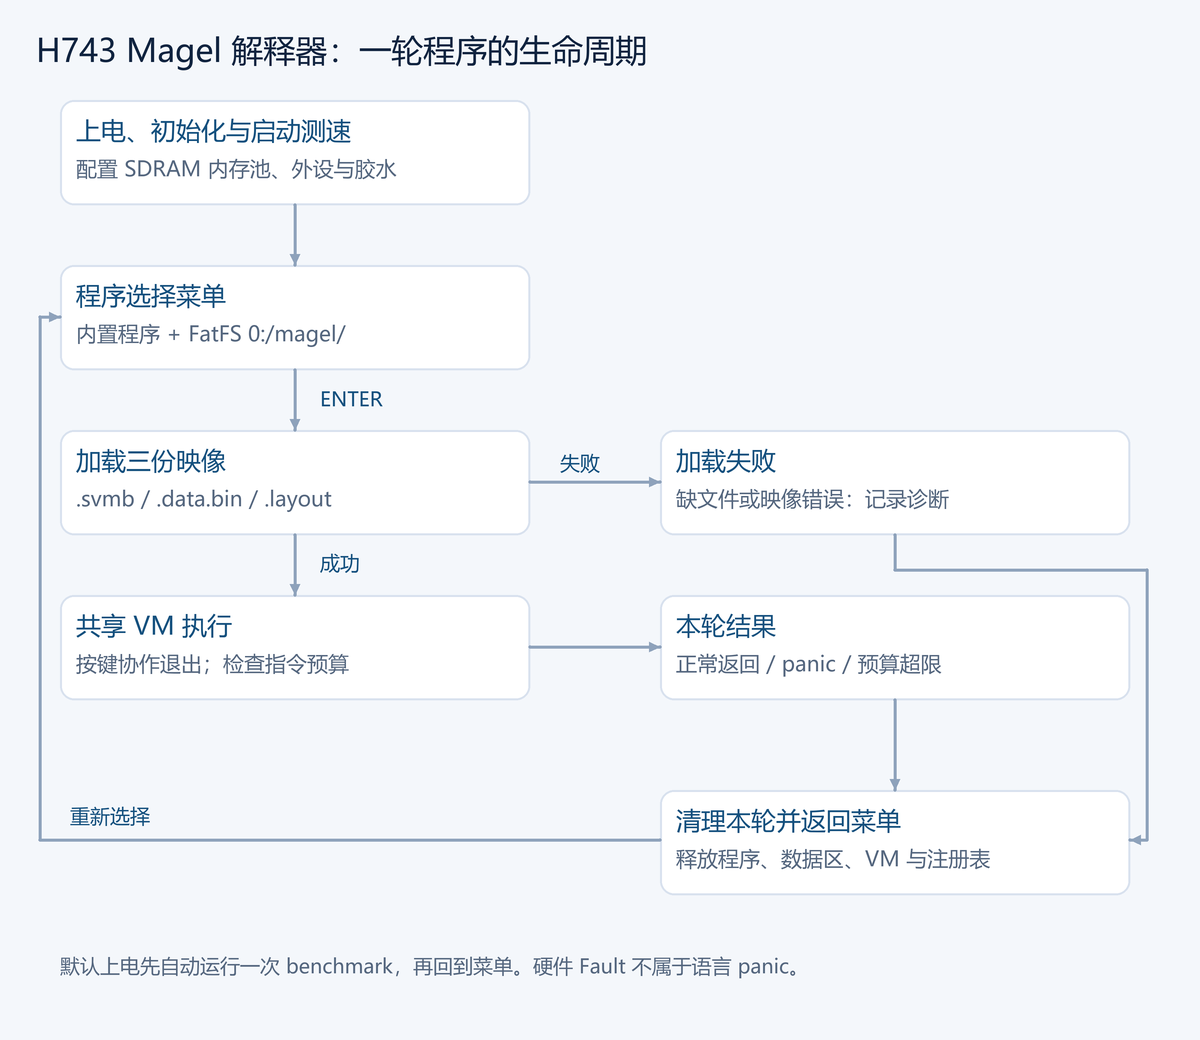
\includegraphics[width=\linewidth]{../images/mcu-execution-flow.png}\par
板端程序从菜单加载、执行到清理返回的生命周期流程
\end{center}

\section{把五个源码入口串起来}

前面的表格是定位地图，下面才是代码的调用关系。读这一套工程时，不要把“共享核心”“桌面 MCU 宿主”和“真实板级入口”当成三个不同的解释器：它们围绕同一个 \texttt{stackvm:\allowbreak{}:\allowbreak{}Machine} 组合出不同的宿主。

\subsection{library/stackvm：程序、数据与执行器分开}

先看 \texttt{stackvm.\allowbreak{}hpp} 的几个公开类型。\texttt{Program} 保存加载后的程序与执行元信息，\texttt{Data\allowbreak{}Area} 保存数据及布局，\texttt{Native\allowbreak{}Registry} 按名字和参数数量登记宿主函数，\texttt{Machine} 才是执行状态与运行时服务的入口。\texttt{Run\allowbreak{}Result} 把成功状态、诊断、执行步数等结果交还宿主。

\texttt{load\allowbreak{}Program\allowbreak{}Binary} 把 \texttt{.\allowbreak{}svmb} 解码为 \texttt{Program}，\texttt{Data\allowbreak{}Area:\allowbreak{}:\allowbreak{}load\allowbreak{}From\allowbreak{}Bytes} 把数据字节和 layout 组合为运行时数据区。二者可以分别失败，所以板端 \texttt{Execute} 给它们安排了独立诊断和返回码，不等到第一条程序指令执行时才猜测“是不是文件读错了”。

\texttt{Machine:\allowbreak{}:\allowbreak{}run} 使用共享的执行核心及其默认优化。源码解析、类型检查和四元式优化已经在桌面编译阶段完成；这里不会再次解释 \texttt{struct}、展开泛型或调用 AOT 编译器。想追具体指令的执行，再从 \texttt{stackvm.\allowbreak{}cpp} 包含的执行模块继续进入寄存器核心与执行准备逻辑。

这层不应直接知道 LCD 型号或 W25QXX 引脚。它通过字节堆、文件 API、输出下沉与原生注册表接收宿主能力，才能同时用于桌面和板端。

\subsection{source/stackvm\_mcu：把桌面服务替换为有预算的宿主}

\texttt{mcu\_host.\allowbreak{}cpp} 是可在桌面运行的 MCU 配置验证入口。它读取映像、安装内存池、挂接输出和原生胶水，再运行同一份字节码。它方便检查裁剪构建、程序结果和软重启，不能由此推断真实 LCD、串口或 SDRAM 已经验证。

把这一目录按职责拆开读会更清楚：

{\small\setlength{\tabcolsep}{4pt}
\begin{longtable}{>{\raggedright\arraybackslash}p{\dimexpr 0.413\linewidth-2\tabcolsep\relax}>{\raggedright\arraybackslash}p{\dimexpr 0.567\linewidth-2\tabcolsep\relax}}
\toprule
文件 & 要解决的具体问题 \\
\midrule
\endhead
\texttt{mcu\_arenas.\allowbreak{}cpp/\allowbreak{}.\allowbreak{}hpp} & 安装元数据、运行时 Arena 与程序字节池，提供当前池与水位 \\
\texttt{mcu\_metadata\_heap.\allowbreak{}cpp} & 为 C++ 元数据分配接入有预算的存储 \\
\texttt{mcu\_glue.\allowbreak{}cpp} & 注册板端基础转换、文本输出等原生函数，并挂接输出下沉 \\
\texttt{mcu\_filesystem.\allowbreak{}hpp}、\texttt{mcu\_file\_api.\allowbreak{}cpp} & 把 VM 文件操作交给宿主文件系统 API \\
\texttt{mcu\_console.\allowbreak{}hpp} & 输入回调约定，供桌面 stdin 或板上串口实现 \\
\bottomrule
\end{longtable}
}

\texttt{Install\allowbreak{}Runtime\allowbreak{}Arena(\allowbreak{})\allowbreak{}} 把 \texttt{Memory:\allowbreak{}:\allowbreak{}} 容器接到指定 Arena，因此应在构造使用这些容器的运行状态之前安装。板级代码先注入元数据与运行时池，安装分配器，再构造字节池的身份索引；顺序变化可能让长期对象先分配到错误的池。

\texttt{mcu\allowbreak{}Glue:\allowbreak{}:\allowbreak{}Register(\allowbreak{}machine,\allowbreak{} \&registry)\allowbreak{}} 把基础胶水注册到指定表，再通过 \texttt{machine.\allowbreak{}set\allowbreak{}Native\allowbreak{}Registry} 交给机器。输出经 \texttt{set\allowbreak{}Output\allowbreak{}Sink} 下沉到宿主，\texttt{keep\allowbreak{}Text=\allowbreak{}false} 时不必把整轮输出积累在 RAM，串口可在运行过程中持续收到文本。

\subsection{板端 main.c：先让硬件能支撑 C++ 宿主}

真实板端的 \texttt{main.\allowbreak{}c} 先关闭中断，配置 MPU、Cache、HAL、系统时钟和 DWT，再初始化定时器、SDRAM、内存管理、串口与按键。打开中断后，输出启动标记，初始化 LCD 与 W25QXX，最后调用 \texttt{Magel\_Board\allowbreak{}Run(\allowbreak{})\allowbreak{}}。

这段顺序解释了为什么不能一上电就创建大容量 VM 容器：外部 SDRAM 与管理器此时还没有就绪。早期少量静态构造的分配由工程明确配置的启动堆承担，之后才切换到外部池。

主入口没有启动电机、舵机和小车任务。\texttt{TIM6\_DAC\_IRQHandler} 提供时基并驱动按键消抖；\texttt{TIM7\_IRQHandler} 只确认参考工程创建的中断。读者修改固件时，应保留这些服务之间的边界，不能因为 SDK 中存在驱动就认为相关任务正在运行。

\subsection{magel\_board.cpp：菜单拥有宿主，Execute 拥有一轮程序}

\texttt{Magel\_Board\allowbreak{}Run} 从 BSP 的外部堆申请三块池，注入元数据与运行时分配器，然后设置字节池、挂载 FatFS、扫描程序并绘制菜单。挂载只尝试读取已有卷，不在失败时格式化介质。

菜单循环维护 \texttt{selected}、\texttt{run} 和 \texttt{last\allowbreak{}Status}。UP/DOWN 改变选择，MODE 重扫，ENTER 把 \texttt{run} 设为真；真正运行发生在下一轮的 \texttt{Execute(\allowbreak{}entries[\allowbreak{}selected]\allowbreak{})\allowbreak{}}。默认启动测速与自检配置也通过这些状态进入执行路径，而不是再维护一套 VM 入口。

\texttt{Execute} 的前半段决定映像来源。内置程序直接引用 Flash 中的指针与长度，外部程序则按同一文件名前缀读取三份 FatFS 文件。\texttt{Read\allowbreak{}File} 检查 1 MiB 上限、实际读取长度和关闭结果；只要一份失败，就返回错误，不偷偷切回内置程序。

解码 \texttt{Program}、加载 \texttt{Data\allowbreak{}Area} 后，实际绑定与执行代码如下，摘自工程：

\par
\medskip
\begin{lstlisting}[style=cpp]
stackvm::NativeRegistry registry;
stackvm::Machine machine;
machine.setHeapAllocator(&mcuArenas::CurrentBytePool());
machine.setData(&data);
machine.setFileApi(&mcuFilesystem::CurrentApi());
mcuGlue::SetOutput(SerialWrite, nullptr, false);
mcuGlue::Register(machine, &registry);
RegisterBoard(registry);
mcuConsole::SetRead(SerialRead, nullptr);
const auto result = machine.run(program, {}, 10000000u);
\end{lstlisting}
\par
\medskip

这里先挂基础胶水，再追加板级接口，两者使用同一个注册表。注册表、数据区和字节池必须在 \texttt{run} 期间有效；\texttt{registry} 比 \texttt{machine} 更早构造，退出作用域时也会更晚析构。字节池是宿主长期提供的对象，不能拿临时池的地址交给机器。

\texttt{Execute} 对读文件、字节码解码、数据加载和执行失败分别返回 2、3、4、5，成功返回 0。菜单接到返回值后记录状态、输出三类池的峰值、清理按键事件并重新绘制界面，因此“运行结束”与“回到可操作菜单”是同一条可追踪路径。

程序、数据区、Machine 和本轮注册表都在 \texttt{Execute} 返回前析构。承载 C++ 静态对象的元数据池却不能直接整块重置，否则仍存在的静态对象会保存失效地址；源码特别保留了这一点。恢复一轮 VM 与清空全部 SDRAM 是不同操作。

\subsection{board.mgl 与 RegisterBoard：名字和实参数量必须对齐}

\texttt{board.\allowbreak{}mgl} 是 Magel 一侧的宿主函数声明，例如：

\par
\medskip
\begin{lstlisting}[style=magel]
void lcdClear(int64 color);
bool boardExitRequested();
void boardDelay(int64 milliseconds);
\end{lstlisting}
\par
\medskip

它们没有 Magel 函数体，编译器按声明检查调用。执行时，\texttt{Register\allowbreak{}Board} 把同名符号绑定到 C++ 回调：

\par
\medskip
\begin{lstlisting}[style=cpp]
registry.add("lcdClear", 1, LcdClear);
registry.add("boardExitRequested", 0, BoardExitRequested);
registry.add("boardDelay", 1, BoardDelay);
\end{lstlisting}
\par
\medskip

声明、名字、参数个数、参数含义和返回值必须同时一致。只在 \texttt{board.\allowbreak{}mgl} 增加声明不会凭空产生硬件能力；只增加 C++ 回调却没有注册，也不能按名字调用。

回调通过 \texttt{Native\allowbreak{}Call\allowbreak{}Context} 读取参数并执行范围检查，再调用 BSP。比如 LCD 要检查颜色与坐标，按键要检查键号。板端禁用 C++ 异常，失败应写入原生调用的错误状态，让 VM 返回失败结果；不能在这里抛异常并期待菜单捕获。

最后沿一个调用自己追一遍：Magel 程序调用 \texttt{lcd\allowbreak{}Clear(\allowbreak{}0)\allowbreak{}}，编译器产生宿主调用，VM 查 \texttt{Native\allowbreak{}Registry} 找到 \texttt{Lcd\allowbreak{}Clear}，回调取整数、检查范围，再调用 LCD 桥接函数。\texttt{println} 则走基础输出下沉到 \texttt{Serial\allowbreak{}Write}。同一套程序逻辑由不同胶水连接到不同宿主，这正是共享核心能够上板的原因。

\section{验证退出与错误恢复}

依次验证：正常返回、主动退出、语言 panic、VM 指令预算超限、缺少数据文件。每轮应释放程序、数据区、VM 与注册表，并回到选择页；默认每轮预算为 10,000,000 条 VM 指令。

硬件 Fault、原生 C/C++ 越界或不可恢复的分配器耗尽不属于语言 panic，不能据此承诺任何错误都能恢复菜单。读代码时应区分 VM 的失败返回和 CPU 的硬件异常。

没有板子时，可先使用桌面上的独立 MCU 宿主回归：

\par
\medskip
\begin{lstlisting}[style=sh]
python tests/mcu_vm.py --magel magel.exe
python tests/mcu_fk_controls.py
python example/mcu/FK-STM32H743XIH6/tools/verify_sdk.py
\end{lstlisting}
\par
\medskip

MCU 宿主回归使用其定义的测试预算，检查裁剪构建、异常符号与选定字节码执行；它不替代 LCD、按键、串口和 SDRAM 的实机测试。板级 README 保留真实硬件的原始测速与恢复记录，历史数据应保留原日期和配置。

做到这里，项目的主线就完整了：同一套语言和 VM 语义，桌面负责生成映像，板端提供受预算约束的宿主，用原生接口接入硬件，并在每轮程序结束后恢复可操作状态。
   % 单片机解释器

\appendix
\chapter{常见错误速查}
\label{ch:appA}

学一门语言，一半时间花在「看懂报错」上。这份附录把本书撰写过程中真跑出来的常见报错收在一起：每条都写清了它长什么样、你为什么踩到、怎么改。

\begin{tip}{提示}
这里的每一条消息都是 Magel 1.0.0 工具链的真实输出（中文本地化）。带 \texttt{<\allowbreak{}!-- fail -->\allowbreak{}} 标记的代码块会在本书的校验脚本里每次都被重跑一遍，所以它们不会随着工具链演进而失真。
\end{tip}

\section{报错的三种长相}

Magel 的报错分三类，看开头几个字就能分清：

{\small\setlength{\tabcolsep}{4pt}
\begin{longtable}{>{\raggedright\arraybackslash}p{\dimexpr 0.372\linewidth-2\tabcolsep\relax}>{\raggedright\arraybackslash}p{\dimexpr 0.293\linewidth-2\tabcolsep\relax}>{\raggedright\arraybackslash}p{\dimexpr 0.315\linewidth-2\tabcolsep\relax}}
\toprule
开头 & 是哪一类 & 什么时候出现 \\
\midrule
\endhead
\texttt{magel：……} & 编译期错误（语义检查） & 运行之前，代码「含义不对」 \\
\texttt{语法错误：文件 第 行第 列：……} & 语法错误 & 运行之前，代码「话都说不通」 \\
\texttt{magel：运行期错误：……} & 运行期错误 & 程序跑到那一句才炸 \\
\bottomrule
\end{longtable}
}

编译期错误和语法错误都不会生成程序，改好再跑就行。运行期错误说明程序编过了、跑起来了，但执行到某一步出了事（除零、越界、\texttt{unwrap} 空值……），后面还会跟着\texttt{出错位置} 和一段 \texttt{调用栈（外 → 内）}，告诉你是哪一行、哪个函数出的事。

一个真实例子，\texttt{1 /\allowbreak{} 0} 跑出来的样子：

\par
\medskip
\begin{lstlisting}[style=magel]
int64 main()
{
    int64 a = 1;
    int64 b = 0;
    println("{}", a / b);
    return 0;
}
\end{lstlisting}
\par
\medskip

\par
\medskip
\begin{lstlisting}[style=out]
magel：运行期错误：整数除零
出错位置：hello.mgl:4（main）
调用栈（外 → 内）：
  main  hello.mgl:4 [thread 0 coroutine 0 ip 12]
\end{lstlisting}
\par
\medskip

从上往下读：先是「整数除零」，再是出错的行号，最后是一份调用栈——\texttt{调用栈（外 → 内）} 意思是从最外层往里读，最后一行是炸掉的那一层。

诊断码。 一部分编译期错误带一个 \texttt{[\allowbreak{}MGLxxxx]\allowbreak{}} 编号（比如下一节的 \texttt{[\allowbreak{}MGL1204]\allowbreak{}}）。编号是稳定的，遇到没见过的错误可以把编号拿去官方文档里搜。

\section{编译期错误速查}

这是你会遇到最多的一类。按「你可能写下的东西」排序：

{\small\setlength{\tabcolsep}{4pt}
\begin{longtable}{>{\raggedright\arraybackslash}p{\dimexpr 0.133\linewidth-2\tabcolsep\relax}>{\raggedright\arraybackslash}p{\dimexpr 0.599\linewidth-2\tabcolsep\relax}>{\raggedright\arraybackslash}p{\dimexpr 0.247\linewidth-2\tabcolsep\relax}}
\toprule
现象 & 真实消息 & 怎么办 \\
\midrule
\endhead
用没声明的变量 & \texttt{magel：引用了没声明的变量：y} & 检查拼写；变量必须先声明再用 \\
调没定义的函数 & \texttt{magel：调用了没定义的函数：nosuch} & 名字拼错，或者忘了 \texttt{import} \\
同一个块里重名 & \texttt{magel：同一个块里不能重复声明：x（要遮蔽外层变量就在内层块里声明）} & 换名字；想遮蔽就用内层块 \\
给 \texttt{const} 赋值 & \texttt{magel：不可变变量（const）不能再赋值：LIMIT} & 去掉 \texttt{const}，或不该在这里改 \\
类型对不上（赋值/返回/传参） & \texttt{magel：不能隐式转换：String ->\allowbreak{} int64（请显式强转）} & 见下面 A.2.1 \\
整数字面量超出目标范围 & \texttt{magel：整数字面量 200 超出 int8 的取值范围（-128.\allowbreak{}.\allowbreak{}127）} & 换类型，或换成范围内的值（见 A.2.2） \\
\texttt{if} 条件不是布尔 & \texttt{magel：if 条件必须是 bool，现在给的是 int64（数值条件请显式写成 }(bool)值\texttt{ 或比较表达式）} & 写比较表达式，别拿数字当布尔 \\
实参个数/类型对不上 & \texttt{magel：调用 函数 f 找不到匹配的重载：(\allowbreak{}int64,\allowbreak{} int64,\allowbreak{} int64)\allowbreak{}；没有参数类型能对上的重载（候选：f）} & 数实参个数；看类型是否精确对上 \\
接口没实现完 & \texttt{magel：struct Circle 实现了接口 Shape，但没有完全实现：area(\allowbreak{})\allowbreak{} ->\allowbreak{} int64（接口要求同名、同返回类型、同形参类型；一个都不能少）} & 把接口里的方法补全，签名一字不差 \\
\texttt{match} 漏了分支 & \texttt{magel：enum match 必须覆盖所有变体或提供 }\_\texttt{ 兜底分支；缺少：Color:\allowbreak{}:\allowbreak{}Green} & 补上缺的变体，或加 \texttt{\_ =\allowbreak{}>\allowbreak{}} 兜底 \\
自定义泛型名撞了内置 & \texttt{magel:\allowbreak{} generics:\allowbreak{} 重复的泛型声明 Pair} & 换个名字（内置有 \texttt{Pair}，改叫 \texttt{Duo} / \texttt{Entry} 之类） \\
找不到模块 & \texttt{magel：模块：找不到模块 no\_such\_module（需要 no\_such\_module.\allowbreak{}mgl）} & 检查 \texttt{import} 的名字与文件是否在同目录 \\
引用声明没初始化 & \texttt{magel：引用声明必须初始化，缺省值请使用 Option<\allowbreak{}T mut\&>\allowbreak{}} & 引用必须当场绑定；可能为空就用 \texttt{Option<\allowbreak{}T mut\&>\allowbreak{}} \\
只读引用被写入 & \texttt{magel：只读引用（}T const\&\texttt{）不能写入元素} & 改用 \texttt{T mut\&} \\
悬垂引用（返回局部引用） & \texttt{magel：[\allowbreak{}MGL1204]\allowbreak{} 返回值中的引用不能超过局部来源的生命周期（int64 mut\&，所属类型 ，来源 local）} & 别把指向局部变量的引用交出去 \\
引用已被释放还在用 & \texttt{magel：[\allowbreak{}MGL1205]\allowbreak{} 借用来源已释放，不能继续访问：表达式} & 检查 \texttt{Drop} / 作用域，别在对象没了以后还用它 \\
\bottomrule
\end{longtable}
}

\subsection{「不能隐式转换」——最高频的一条}

九成的类型报错都是这一句。先记住第 3 章 3.8 节的规矩：Magel 只放行「装得下」的方向。下面这几种会自动放行（不用签字）：

\begin{center}
\begin{tabular}{ll}
\toprule
方向 & 例子 \\
\midrule
同符号整型变宽 & \texttt{int8 → int64}、\texttt{int32 → int64}、\texttt{uint8 → uint32} \\
无符号 \ensuremath{\rightarrow} 更宽的有符号 & \texttt{uint8 → int32}、\texttt{uint32 → int64} \\
整型 \ensuremath{\rightarrow} 浮点 & \texttt{int64 → float64}、\texttt{int32 → float32} \\
浮点变宽 & \texttt{float32 → float64} \\
\bottomrule
\end{tabular}
\end{center}

反方向一律要显式强转 \texttt{(\allowbreak{}目标类型)\allowbreak{}值}。最常见的四种：

\par
\medskip
\begin{lstlisting}[style=magel]
int64 main()
{
    int64 big = 70000;
    int32 small = big;
    // 缩窄：位宽变小
    println("{}", small);
    return 0;
}
\end{lstlisting}
\par
\medskip

\par
\medskip
\begin{lstlisting}[style=out]
magel：不能隐式转换：int64 -> int32（请显式强转）
\end{lstlisting}
\par
\medskip

\begin{itemize}

\item 缩窄（位宽变小）：\texttt{int64 → int32}、\texttt{float64 → float32}、\texttt{uint8 → int8} \ensuremath{\rightarrow} 写 \texttt{(\allowbreak{}int32)\allowbreak{}big}

\item 有符号 \ensuremath{\rightarrow} 无符号：\texttt{int32 → uint32}、\texttt{int64 → uint64}（目标更宽也不行，负数塞不进去）\ensuremath{\rightarrow} 写 \texttt{(\allowbreak{}uint32)\allowbreak{}x}

\item 跨大类：\texttt{float64 → int64}、\texttt{char}/\texttt{bool} \ensuremath{\leftrightarrow} \texttt{int64} \ensuremath{\rightarrow} 写 \texttt{(\allowbreak{}int64)\allowbreak{}f}

\item 浮点字面量：\texttt{float32 f =\allowbreak{} 1.\allowbreak{}5;} 里的 \texttt{1.\allowbreak{}5} 是 \texttt{float64}，往更窄的 \texttt{float32} 放也要签字 \ensuremath{\rightarrow} \texttt{(\allowbreak{}float32)\allowbreak{}1.\allowbreak{}5}

\end{itemize}

\begin{tip}{提示}
\texttt{+} 号在谁身上，谁就有错。 读这条报错只要看箭头两边：左边是「你给的」，右边是「它想要的」，改左边（强转）或者右边（换类型）都行。
\end{tip}

\subsection{「整数字面量超出取值范围」}

这是「字面量落进槽位」时独立的一道检查——十进制字面量的值装不进目标整型就报错：

\par
\medskip
\begin{lstlisting}[style=magel]
int64 main()
{
    uint8 b = 256;
    // uint8 只到 255
    return 0;
}
\end{lstlisting}
\par
\medskip

\par
\medskip
\begin{lstlisting}[style=out]
magel：整数字面量 256 超出 uint8 的取值范围（0..255）
\end{lstlisting}
\par
\medskip

规矩（第 3 章 3.10 节）：

\begin{itemize}

\item \texttt{uint8 b =\allowbreak{} 255;} \textcolor{green!50!black}{\ding{51}}（在 \texttt{0.\allowbreak{}.\allowbreak{}255} 里）、\texttt{int16 s =\allowbreak{} -300;} \textcolor{green!50!black}{\ding{51}}（在 \texttt{-32768.\allowbreak{}.\allowbreak{}32767} 里）；

\item \texttt{uint8 b =\allowbreak{} 256;} \textcolor{red!80!black}{\ding{55}}、\texttt{int8 x =\allowbreak{} 200;} \textcolor{red!80!black}{\ding{55}} —— 不再静默回绕；

\item \texttt{0x} / \texttt{b} 前缀的字面量按位模式放行（\texttt{int8 x =\allowbreak{} 0x\allowbreak{}FF;} 得到 \texttt{-1}），不做范围检查；

\item 显式强转不走这条检查：\texttt{(\allowbreak{}uint8)\allowbreak{}256} 得到 \texttt{0}，是你签字的结果。

\end{itemize}

\subsection{引用相关的错，多在「生命周期」上}

引用一共就两类错，认清就能改：

第一类：引用没绑定就声明。 Magel 没有空引用：

\par
\medskip
\begin{lstlisting}[style=magel]
int64 main()
{
    int64 mut& r = 5;
    // 引用要从对象身上取地址，不能绑字面量
    return 0;
}
\end{lstlisting}
\par
\medskip

\par
\medskip
\begin{lstlisting}[style=out]
magel：不能隐式转换：int64 -> int64 mut&（请显式强转）
\end{lstlisting}
\par
\medskip

改成绑定一个确实存在的对象：\texttt{int64 x =\allowbreak{} 5; int64 mut\& r =\allowbreak{} \&x;}。

第二类：引用活得比目标久。 编译期就会拦：

\par
\medskip
\begin{lstlisting}[style=magel]
int64 main()
{
    int64 mut& r;
    println("{}", r);
    return 0;
}
\end{lstlisting}
\par
\medskip

\par
\medskip
\begin{lstlisting}[style=out]
magel：引用声明必须初始化，缺省值请使用 Option<T mut&>
\end{lstlisting}
\par
\medskip

把指向局部变量的引用返回出去，报的是 \texttt{[\allowbreak{}MGL1204]\allowbreak{}}：

\par
\medskip
\begin{lstlisting}[style=out]
magel：[MGL1204] 返回值中的引用不能超过局部来源的生命周期（int64 mut&，所属类型 ，来源 local）
\end{lstlisting}
\par
\medskip

规矩只有一条：来源必须比引用活得久。来源是参数、是调用方给的，就安全；来源是本函数的局部变量，就不行。详细展开见\hyperref[ch:07]{第 7 章}。

\section{语法错误速查}

语法错误长这样：\texttt{语法错误：文件 第 行第 列：期望 ……，实际是 ……}，并且会画出出错位置和一个小波浪线 \texttt{\textasciitilde{}\textasciitilde{}\textasciitilde{}\textasciitilde{}}。消息里的记号名（\texttt{条件(\allowbreak{}if)\allowbreak{}}、\texttt{分号(\allowbreak{};)\allowbreak{}} 之类）都是中文，照着它说的补就行，行列号也是准的。

{\small\setlength{\tabcolsep}{4pt}
\begin{longtable}{>{\raggedright\arraybackslash}p{\dimexpr 0.079\linewidth-2\tabcolsep\relax}>{\raggedright\arraybackslash}p{\dimexpr 0.743\linewidth-2\tabcolsep\relax}>{\raggedright\arraybackslash}p{\dimexpr 0.158\linewidth-2\tabcolsep\relax}}
\toprule
现象 & 真实消息 & 怎么办 \\
\midrule
\endhead
语句少写分号 & \texttt{语法错误：x.\allowbreak{}mgl 第 3 行第 5 列：期望 条件(\allowbreak{}if)\allowbreak{} /\allowbreak{} 自增(\allowbreak{}++)\allowbreak{} /\allowbreak{} 自减(\allowbreak{}--)\allowbreak{} /\allowbreak{} 加号(\allowbreak{}+)\allowbreak{} 等 44 个之一，实际是 返回(\allowbreak{}return)\allowbreak{}} & 看行号，上一句末尾补 \texttt{;} \\
\bottomrule
\end{longtable}
}

类型声明的尾部分号是可选的：\texttt{struct}、\texttt{enum}、\texttt{interface} 在 \texttt{\}} 结束，可以再写 \texttt{;}，也可以不写。不要把合法的省略分号误当成错误；普通声明、赋值、返回和 \texttt{do .\allowbreak{}.\allowbreak{}.\allowbreak{} while} 的分号仍然要保留。

\par
\medskip
\begin{lstlisting}[style=magel]
struct Point
{
    int64 x;
    int64 y;
}

int64 main()
{
    Point point;
    println("{}", point.x);
    return 0;
}
\end{lstlisting}
\par
\medskip

\par
\medskip
\begin{lstlisting}[style=out]
0
\end{lstlisting}
\par
\medskip

其它几条词法/语法坑（第 3 章 3.10 节实测过）：

\begin{center}
\begin{tabular}{lll}
\toprule
你可能想写 & 实际会怎样 & 改成 \\
\midrule
\texttt{0b1010} & 词法错误（前缀是 \texttt{b}） & \texttt{b1010} \\
\texttt{1\_000} & 语法错误（下划线分隔不认） & \texttt{1000} \\
\texttt{1.\allowbreak{}0F} / \texttt{1U} & 后缀必须小写 & \texttt{1.\allowbreak{}0f} / \texttt{1u} \\
\bottomrule
\end{tabular}
\end{center}

\section{运行期错误速查}

运行期错误都带 \texttt{magel：运行期错误：} 前缀，后面跟具体原因、出错位置和调用栈。它们不是「未定义行为」，是明确被检查到的错误——出问题的那一下，程序会停下来告诉你，而不是悄悄读到垃圾数据。

\begin{center}
\begin{tabular}{ll}
\toprule
现象 & 真实消息（首行） \\
\midrule
整数除以零 & \texttt{magel：运行期错误：整数除零} \\
定长数组越界 & \texttt{magel：运行期错误：数组下标越界：fixed 的下标 5，长度 3} \\
\texttt{List} 越界 & \texttt{magel：运行期错误：vec 下标越界：5（长度 1）} \\
展开空的 \texttt{Option} & \texttt{magel：运行期错误：panic：called Option.\allowbreak{}unwrap(\allowbreak{})\allowbreak{} on None} \\
展开 \texttt{Err} 的 \texttt{Result} & \texttt{magel：运行期错误：panic：called Result.\allowbreak{}unwrap(\allowbreak{})\allowbreak{} on Err} \\
\texttt{expect} 落空 & \texttt{magel：运行期错误：panic：<\allowbreak{}你写的消息>\allowbreak{}} \\
\texttt{assert} 失败 & \texttt{magel：运行期错误：panic：<\allowbreak{}你写的消息>\allowbreak{}} \\
主动 \texttt{panic} & \texttt{magel：运行期错误：panic：<\allowbreak{}你写的消息>\allowbreak{}} \\
\bottomrule
\end{tabular}
\end{center}

\texttt{unwrap} 空 \texttt{Option}，一次看清楚它长什么样：

\par
\medskip
\begin{lstlisting}[style=magel]
int64 main()
{
    Option<int64> none = None;
    println("{}", none.unwrap());
    return 0;
}
\end{lstlisting}
\par
\medskip

\par
\medskip
\begin{lstlisting}[style=out]
magel：运行期错误：panic：called Option.unwrap() on None
\end{lstlisting}
\par
\medskip

\begin{tip}{提示}
注意区分两种「空」。 \texttt{Option<\allowbreak{}int64>\allowbreak{} none;}（默认构造）不是空——它的 \texttt{is\allowbreak{}None(\allowbreak{})\allowbreak{}} 是 \texttt{0}，里面装的是默认值 \texttt{0}。真正的空要显式写\texttt{Option<\allowbreak{}int64>\allowbreak{} none =\allowbreak{} None;}，这时 \texttt{is\allowbreak{}None(\allowbreak{})\allowbreak{}} 才是 \texttt{1}。第 16 章讲过这个区别。所以 \texttt{unwrap} 报错的是「\texttt{=\allowbreak{} None} 那种空」，不是随便一个 \texttt{Option} 变量。
\end{tip}

越界的两条消息措辞不同（一个是数组、一个是 \texttt{List}），别以为是两种错：

\par
\medskip
\begin{lstlisting}[style=out]
magel：运行期错误：数组下标越界：fixed 的下标 5，长度 3     <- 定长数组，带变量名
magel：运行期错误：vec 下标越界：5（长度 1）                <- List
\end{lstlisting}
\par
\medskip

\section{工具链与工程错误}

{\small\setlength{\tabcolsep}{4pt}
\begin{longtable}{>{\raggedright\arraybackslash}p{\dimexpr 0.156\linewidth-2\tabcolsep\relax}>{\raggedright\arraybackslash}p{\dimexpr 0.530\linewidth-2\tabcolsep\relax}>{\raggedright\arraybackslash}p{\dimexpr 0.294\linewidth-2\tabcolsep\relax}}
\toprule
现象 & 真实消息 & 怎么办 \\
\midrule
\endhead
用了注解/反射但工具链不支持 & \texttt{magel：x.\allowbreak{}mgl 第 1 行第 1 列：注解与反射功能未开启，请使用支持该能力的工具链及 --reflection} & 用带反射的构建，运行时加 \texttt{--reflection}（第 20 章） \\
调了不存在的方法 & \texttt{magel：方法只能调在 struct 上：foo\allowbreak{}Bar} & 方法名拼错，或那个类型上真没有这个方法 \\
嵌入模式用了被禁的能力 & （编译期门禁） & 见\hyperref[ch:22]{第 22 章}的 \texttt{[\allowbreak{}embedded]\allowbreak{}} 一节 \\
\bottomrule
\end{longtable}
}

\texttt{方法只能调在 struct 上：xxx} 这条措辞有误导性：它不是说「你不能在 struct 上调方法」，而是说「你调的这个方法没找到」。看到它，先回去核对方法名。

反射那条同理——不是你的代码错，是工具链没开那个功能。本书第 20 章的所有例子都得靠一个开了反射的工具链来跑，默认构建会直接拒绝。

\section{排查五步法}

卡住了，按这个顺序走，八成能自己解决：

\begin{enumerate}

\item 看开头几个字，定类别：\texttt{语法错误} \ensuremath{\rightarrow} 语法；\texttt{magel：} \ensuremath{\rightarrow} 编译期；\texttt{magel：运行期错误：} \ensuremath{\rightarrow} 运行期。三类改法完全不同。

\item 语法/编译期：看行号，往上一行找。 报错行常常只是「被发现」的地方，真正的问题往往在上一行（典型的：少分号）。

\item 类型报错：读箭头。 \texttt{不能隐式转换：A ->\allowbreak{} B} 就是「你给了 A，它要 B」。要么强转左边，要么把右边换成 A。

\item 引用报错：问「来源是谁」。 来源是本函数的局部变量吗？是就错在这；来源是参数、是更长命的对象吗？那就是别的地方。

\item 还是不懂：拿消息关键词去查。 消息里的中文（比如「只读引用」）和诊断码（\texttt{[\allowbreak{}MGL1204]\allowbreak{}}）都能拿去文档或代码里搜——这套消息是刻意写清楚给人看的。

\end{enumerate}

\section{下一步}

错误看得懂，剩下就是写。翻到\hyperref[ch:appB]{附录 B}，按能力域认识一遍标准库；或者回到\hyperref[ch:23]{第 23 章}，拿一个完整项目把学到的东西串起来。
   % 常见错误速查
\chapter{标准库速查}
\label{ch:appB}

Magel 的「标准库」不是一堆函数，而是一组模块：除核心 \texttt{std:\allowbreak{}:\allowbreak{}lang} 自动加载外，其余都得先 \texttt{import}。这份附录按能力域把它们列一遍，让你知道「想干这件事，该去 \texttt{import} 谁」；每个模块的完整签名与错误边界，去\href{https://github.com/rabbitc999/Magel/blob/master/doc/library/README.md}{库函数 API 参考}查。

\begin{tip}{提示}
模块名与方法对齐 Magel 1.0.0。终端中可以直接用 \texttt{magel man} 查模块，用\texttt{magel man 模块:\allowbreak{}:\allowbreak{}符号} 查签名、说明和示例；命令说明见 \href{https://github.com/rabbitc999/Magel/blob/master/doc/man/README.md}{doc/man}。
\end{tip}

\section{先看一个例子}

\par
\medskip
\begin{lstlisting}[style=magel]
import std::math;
import std::text;
import std::iter;

int64 main()
{
    println("sqrt={}", std::math::sqrt(144.0));
    println("upper={}", std::text::Text::toUpper("magel"));
    int64 sum = 0;
    for (int64 v in std::iter::range(1, 5))
    {
        sum += v;
    }
    println("sum={}", sum);
    return 0;
}
\end{lstlisting}
\par
\medskip

\par
\medskip
\begin{lstlisting}[style=out]
sqrt=12
upper=MAGEL
sum=10
\end{lstlisting}
\par
\medskip

三行分别来自三个模块：数学、文本、迭代。注意 \texttt{range(\allowbreak{}1,\allowbreak{} 5)\allowbreak{}} 是左闭右开 （拿到 1、2、3、4），所以 \texttt{sum} 是 10——这是第 17 章的规矩，标准库里凡带「起点、终点」的地方都一样。

\section{核心模块 \texttt{std:\allowbreak{}:\allowbreak{}lang}（不用 import）}

这几样任何程序里都能直接用：

\begin{center}
\begin{tabular}{ll}
\toprule
能力 & 用法 \\
\midrule
输出 & \texttt{println(\allowbreak{}fmt,\allowbreak{} …)\allowbreak{}}、\texttt{format(\allowbreak{}fmt,\allowbreak{} …)\allowbreak{}} \\
断言 & \texttt{assert(\allowbreak{}cond)\allowbreak{}} \\
取长度 & \texttt{len(\allowbreak{}x)\allowbreak{}}（字符串 / 容器） \\
字符串 & \texttt{std:\allowbreak{}:\allowbreak{}lang:\allowbreak{}:\allowbreak{}String} \\
容器 & \texttt{List<\allowbreak{}T>\allowbreak{}}、\texttt{Map<\allowbreak{}K,\allowbreak{}V>\allowbreak{}}、\texttt{Set<\allowbreak{}T>\allowbreak{}} \\
类型擦除盒子 & \texttt{std:\allowbreak{}:\allowbreak{}lang:\allowbreak{}:\allowbreak{}Any}（第 13 章的运行期多态） \\
数学常数 & \texttt{std:\allowbreak{}:\allowbreak{}lang:\allowbreak{}:\allowbreak{}Math:\allowbreak{}:\allowbreak{}PI}、\texttt{std:\allowbreak{}:\allowbreak{}lang:\allowbreak{}:\allowbreak{}Math:\allowbreak{}:\allowbreak{}E} \\
大数 & \texttt{Big\allowbreak{}Integer}、\texttt{Big\allowbreak{}Decimal} \\
输入 & \texttt{input(\allowbreak{}variable)\allowbreak{}} \\
整行输入 & \texttt{std:\allowbreak{}:\allowbreak{}lang:\allowbreak{}:\allowbreak{}read\allowbreak{}Line(\allowbreak{})\allowbreak{}}，保留空格，不含 LF/CRLF \\
多行输入 & \texttt{std:\allowbreak{}:\allowbreak{}lang:\allowbreak{}:\allowbreak{}read\allowbreak{}Lines(\allowbreak{}int32 N)\allowbreak{}}，LF 连接，EOF 提前结束 \\
\bottomrule
\end{tabular}
\end{center}

\begin{tip}{提示}
早年间它们不在 \texttt{lang} 里也能用（靠 \texttt{source/\allowbreak{}std/\allowbreak{}lang.\allowbreak{}mgl} 注入正文）。现在除了上面这些，其它能力一律要显式 \texttt{import}——这是第 18 章「模块与工程」讲过的变化。
\end{tip}

\section{按能力域速查}

\subsection{数学与数值}

{\small\setlength{\tabcolsep}{4pt}
\begin{longtable}{>{\raggedright\arraybackslash}p{\dimexpr 0.108\linewidth-2\tabcolsep\relax}>{\raggedright\arraybackslash}p{\dimexpr 0.872\linewidth-2\tabcolsep\relax}}
\toprule
模块 & 能干什么 \\
\midrule
\endhead
\texttt{std:\allowbreak{}:\allowbreak{}math} & \texttt{sin} \texttt{cos} \texttt{sqrt} 等常用函数；\texttt{abs} \texttt{min} \texttt{max} 是泛型入口，\texttt{min}/\texttt{max} 可以给任意多个实参（常数见 \texttt{std:\allowbreak{}:\allowbreak{}lang:\allowbreak{}:\allowbreak{}Math}） \\
\texttt{std:\allowbreak{}:\allowbreak{}numerics} & 标量数值方法：导数、辛普森积分、二分、RK4、牛顿迭代 \\
\texttt{std:\allowbreak{}:\allowbreak{}numtheory} & 整数数论：模块级泛型 \texttt{gcd} \texttt{lcm}（任意多个实参）、\texttt{add\allowbreak{}Mod} \texttt{mul\allowbreak{}Mod} \texttt{pow\allowbreak{}Mod} \texttt{mod\allowbreak{}Inverse}，以及确定性的 \texttt{is\allowbreak{}Prime}（Miller-Rabin） \\
\texttt{std:\allowbreak{}:\allowbreak{}complex} & 复数 \texttt{Complex<\allowbreak{}T>\allowbreak{}}，加减乘除都是一等公民 \\
\texttt{std:\allowbreak{}:\allowbreak{}linalg} & 稠密向量与矩阵：\texttt{lu\allowbreak{}Decompose} \texttt{symmetric\allowbreak{}Eigen} \texttt{svd} \texttt{jordan2} \texttt{diagonalize2} \\
\texttt{std:\allowbreak{}:\allowbreak{}random} & 确定性随机数（LCG）与熵播种；句柄型状态，实现 \texttt{Drop} \\
\texttt{std:\allowbreak{}:\allowbreak{}signal} & DFT / FFT 与逆变换；基 2 的 FFT 只接受 2 的幂长度 \\
\bottomrule
\end{longtable}
}

\subsection{文本与数据格式}

{\small\setlength{\tabcolsep}{4pt}
\begin{longtable}{>{\raggedright\arraybackslash}p{\dimexpr 0.140\linewidth-2\tabcolsep\relax}>{\raggedright\arraybackslash}p{\dimexpr 0.840\linewidth-2\tabcolsep\relax}}
\toprule
模块 & 能干什么 \\
\midrule
\endhead
\texttt{std:\allowbreak{}:\allowbreak{}text} & \texttt{Text:\allowbreak{}:\allowbreak{}find} \texttt{split} \texttt{join} \texttt{replace} \texttt{trim} \texttt{to\allowbreak{}Upper} \texttt{pad\allowbreak{}Start} …… \\
\texttt{std:\allowbreak{}:\allowbreak{}json} & \texttt{parse} \ensuremath{\rightarrow} \texttt{Result<\allowbreak{}Json\allowbreak{}Value,\allowbreak{} String>\allowbreak{}}；再 \texttt{is\allowbreak{}Int} \texttt{is\allowbreak{}Object} \texttt{len} \texttt{as\allowbreak{}Int} \texttt{as\allowbreak{}String} 取值 \\
\texttt{std:\allowbreak{}:\allowbreak{}toml} & 与 json 同构的 TOML 文档访问 \\
\texttt{std:\allowbreak{}:\allowbreak{}regex} & 正则；模式缓存在宿主侧，Magel 侧只拿一个整数句柄 \\
\texttt{std:\allowbreak{}:\allowbreak{}parse} & 字符串 \ensuremath{\rightarrow} 整数，失败给 \texttt{Parse\allowbreak{}Error} \\
\texttt{std:\allowbreak{}:\allowbreak{}binary} & 定宽解码、字节序处理与边界检查 \\
\texttt{std:\allowbreak{}:\allowbreak{}path} & 路径拼接、取文件名、取扩展名、规范化 \\
\texttt{std:\allowbreak{}:\allowbreak{}compress} & 文本压缩 / 解压；压缩结果是二进制 \texttt{List<\allowbreak{}uint8>\allowbreak{}} \\
\bottomrule
\end{longtable}
}

\subsection{并发与协作}

\begin{center}
\begin{tabular}{ll}
\toprule
模块 & 能干什么 \\
\midrule
\texttt{std:\allowbreak{}:\allowbreak{}coroutine} & 共享协程 \\
\texttt{std:\allowbreak{}:\allowbreak{}thread} & 隔离线程 \texttt{Isolated\allowbreak{}Thread} \\
\texttt{std:\allowbreak{}:\allowbreak{}message} & 跨协程 / 跨线程的消息 \\
\texttt{std:\allowbreak{}:\allowbreak{}concurrency} & 显式共享槽 \texttt{Shared<\allowbreak{}T>\allowbreak{}}（普通全局变量在线程间仍是隔离的） \\
\texttt{std:\allowbreak{}:\allowbreak{}event} & 中断事件与软件定时器；\texttt{start(\allowbreak{})\allowbreak{}} 后按周期在指令边界触发 \\
\bottomrule
\end{tabular}
\end{center}

\begin{tip}{提示}
\texttt{Shared\allowbreak{}Coroutine} / \texttt{Isolated\allowbreak{}Thread} / \texttt{Message} 是三个独立模块，不能合并——它们各自有同名的宿主函数 \texttt{create} / \texttt{wait} / \texttt{receive}。
\end{tip}

\subsection{系统与环境}

{\small\setlength{\tabcolsep}{4pt}
\begin{longtable}{>{\raggedright\arraybackslash}p{\dimexpr 0.136\linewidth-2\tabcolsep\relax}>{\raggedright\arraybackslash}p{\dimexpr 0.844\linewidth-2\tabcolsep\relax}}
\toprule
模块 & 能干什么 \\
\midrule
\endhead
\texttt{std:\allowbreak{}:\allowbreak{}io} & 文件读写；错误类型 \texttt{Io\allowbreak{}Error}（\texttt{Open\allowbreak{}Failed} \texttt{Read\allowbreak{}Failed} \texttt{Write\allowbreak{}Failed} \texttt{Seek\allowbreak{}Failed} \texttt{Closed}） \\
\texttt{std:\allowbreak{}:\allowbreak{}net} & TCP 与极简 HTTP 客户端；套接字在宿主胶水里，Magel 侧只拿 \texttt{int32} 句柄 \\
\texttt{std:\allowbreak{}:\allowbreak{}sql} & 连 MySQL / SQLite / PostgreSQL / SQL Server；SQL 交给数据库引擎执行 \\
\texttt{std:\allowbreak{}:\allowbreak{}process} & 进程与系统调用；命令管道由宿主管柄池持有 \\
\texttt{std:\allowbreak{}:\allowbreak{}clock} & 单调时钟 \texttt{steady\_clock}，只用来做差值，别当挂钟用 \\
\texttt{std:\allowbreak{}:\allowbreak{}memory} & \texttt{Span<\allowbreak{}T>\allowbreak{}}（指针 + 长度视图）；它的迭代器给的是元素指针，能直接写 \\
\texttt{std:\allowbreak{}:\allowbreak{}watchdog} & 软重启看门狗（水位与超时两个维度都默认关闭），桌面与板端共用一份实现 \\
\bottomrule
\end{longtable}
}

\subsection{迭代}

\begin{center}
\begin{tabular}{ll}
\toprule
模块 & 能干什么 \\
\midrule
\texttt{std:\allowbreak{}:\allowbreak{}iter} & \texttt{range}、\texttt{map} / \texttt{filter} / \texttt{collect} 惰性链，以及 \texttt{Iter\allowbreak{}Next<\allowbreak{}T>\allowbreak{}} 接口 \\
\bottomrule
\end{tabular}
\end{center}

\begin{tip}{提示}
\texttt{std:\allowbreak{}:\allowbreak{}probe} 是测试用的桩模块，不是给应用用的。
\end{tip}

\section{三条容易踩的约定}

一、句柄型资源要显式关。 \texttt{std:\allowbreak{}:\allowbreak{}json}、\texttt{std:\allowbreak{}:\allowbreak{}regex}、\texttt{std:\allowbreak{}:\allowbreak{}sql} 这类持有宿主资源的值，用 \texttt{close(\allowbreak{})\allowbreak{}} 关，或者让它实现 \texttt{Closeable}、由作用域替你关（第 8 章）。重复关闭返回 \texttt{false}，不会崩。

二、压缩结果是二进制，不是文本。 \texttt{std:\allowbreak{}:\allowbreak{}compress} 的输出含 \texttt{\textbackslash\{\}0} 字节，类型是\texttt{std:\allowbreak{}:\allowbreak{}lang:\allowbreak{}:\allowbreak{}List<\allowbreak{}uint8>\allowbreak{}}；别拿它当字符串打印，解压出来的才是 \texttt{std:\allowbreak{}:\allowbreak{}lang:\allowbreak{}:\allowbreak{}String}。

三、前端嵌入式配置固定禁用部分模块。 \texttt{std:\allowbreak{}:\allowbreak{}net}、\texttt{std:\allowbreak{}:\allowbreak{}process}、\texttt{std:\allowbreak{}:\allowbreak{}sql}、\texttt{std:\allowbreak{}:\allowbreak{}io}、\texttt{std:\allowbreak{}:\allowbreak{}thread}、\texttt{std:\allowbreak{}:\allowbreak{}coroutine}、\texttt{std:\allowbreak{}:\allowbreak{}concurrency} 在 \texttt{[\allowbreak{}embedded]\allowbreak{}} 目标下\texttt{import} 就会编译报错——不是你的代码写错了，是那一端不提供这个能力。见第 22 章。

\section{细节去哪儿查}

{\small\setlength{\tabcolsep}{4pt}
\begin{longtable}{>{\raggedright\arraybackslash}p{\dimexpr 0.318\linewidth-2\tabcolsep\relax}>{\raggedright\arraybackslash}p{\dimexpr 0.662\linewidth-2\tabcolsep\relax}}
\toprule
你想查 & 去哪 \\
\midrule
\endhead
某个函数的确切签名、默认值、返回与错误 & \href{https://github.com/rabbitc999/Magel/blob/master/doc/library/README.md}{库函数 API 参考} 与\href{https://github.com/rabbitc999/Magel/blob/master/doc/library/symbols.md}{全部函数索引} \\
按能力域通读一遍标准库 & \href{https://github.com/rabbitc999/Magel/blob/master/doc/07-stdlib-overview.md}{07 标准库概览} \\
标准库源码（每个模块头部都有能力说明） & \href{https://github.com/rabbitc999/Magel/tree/master/source/std}{\texttt{source/\allowbreak{}std/\allowbreak{}}} 下的 \texttt{source/\allowbreak{}std/\allowbreak{}<\allowbreak{}名字>\allowbreak{}.\allowbreak{}mgl} \\
宿主侧绑定（\texttt{std:\allowbreak{}:\allowbreak{}*} 的真正实现） & \href{https://github.com/rabbitc999/Magel/tree/master/source/glue}{\texttt{source/\allowbreak{}glue/\allowbreak{}}} 下的 \texttt{source/\allowbreak{}glue/\allowbreak{}std\_*.\allowbreak{}hpp} \\
可直接运行的标准库样例 & \href{https://github.com/rabbitc999/Magel/tree/master/example/samples}{\texttt{example/\allowbreak{}samples/\allowbreak{}}} \\
\bottomrule
\end{longtable}
}

\begin{tip}{模块名怎么读}
\texttt{std:\allowbreak{}:\allowbreak{}json} 对应源码 \texttt{source/\allowbreak{}std/\allowbreak{}json.\allowbreak{}mgl}、胶水 \texttt{source/\allowbreak{}glue/\allowbreak{}std\_json.\allowbreak{}hpp}，三处名字一对就找到了。
\end{tip}

\section{下一步}

标准库认完了，前面二十几章也读完了——接下来该自己写点东西了。

\begin{itemize}

\item 想先复习报错怎么读：翻回\hyperref[ch:appA]{附录 A}；

\item 想把整本书的东西拼成一个完整程序：\hyperref[ch:23]{第 23 章 综合项目}；

\item 想把这门语言接到你自己的 C/C++ 代码上：\hyperref[ch:21]{第 21 章 与 C 互操作}。

\end{itemize}
   % 标准库速查

\end{document}
